% Eriq Augustine
%
% Cal Poly Thesis
%
% based on UC Thesis format
%
% modified by Mark Barry 2/07.
%

\documentclass[12pt]{ucthesis}

\usepackage[hyphens]{url}
\usepackage{hyperref}
\usepackage{subfig}
\usepackage{graphicx}
\usepackage{amssymb}
\usepackage{amsmath}
\usepackage[letterpaper]{geometry}
\usepackage[overload]{textcase}
\usepackage{color}
\usepackage[nonumberlist,toc]{glossaries}
\usepackage{wrapfig}
\usepackage{longtable}
\usepackage{morefloats}
\usepackage{float}
\usepackage{listings}
\usepackage{makecell}

\definecolor{orange}{rgb}{1,0.5,0}
\definecolor{blue}{rgb}{0.1,0.1,0.8}
\definecolor{green}{rgb}{0,0.5,0}
\definecolor{red}{rgb}{0.8,0,0}
\definecolor{bad}{rgb}{0.8,0,0.8}

\makeindex
\makeglossaries

\bibliographystyle{abbrv}

\setlength{\parindent}{0.25in} \setlength{\parskip}{6pt}
\geometry{verbose,nohead,tmargin=1.25in,bmargin=1in,lmargin=1.5in,rmargin=1.3in}
\setcounter{tocdepth}{2}

% Different font in captions (single-spaced, bold) ------------
\newcommand{\captionfonts}{\small\bf\ssp}

\makeatletter  % Allow the use of @ in command names
\long\def\@makecaption#1#2{%
  \vskip\abovecaptionskip
  \sbox\@tempboxa{{\captionfonts #1: #2}}%
  \ifdim \wd\@tempboxa >\hsize
    {\captionfonts #1: #2\par}
  \else
    \hbox to\hsize{\hfil\box\@tempboxa\hfil}%
  \fi
  \vskip\belowcaptionskip}
\makeatother   % Cancel the effect of \makeatletter
% ---------------------------------------

\begin{document}

% Declarations for Front Matter

% Update fields below!
\title{SPOONS: Netflix Outage Detection Using Microtext Classification}
\author{Eriq Augustine}
\degreemonth{March} \degreeyear{2012} \degree{Master of Science}
\defensemonth{March} \defenseyear{2012}
\numberofmembers{3} \chair{Alex Dekhtyar, Ph.D.} \othermemberA{Clint Staley, Ph.D.} \othermemberB{Franz Kurfess, Ph.D.} \othermemberC{Foaad Khosmood, Ph.D.} \field{Computer Science} \campus{San Luis Obispo}
\copyrightyears{seven}

\maketitle

\begin{frontmatter}

% Custom made for Cal Poly (by Mark Barry, modified by Andrew Tsui).
\copyrightpage

% Custom made for Cal Poly (by Andrew Tsui).
\committeemembershippage

\begin{abstract}

Every week there are over a billion new posts to Twitter services and many of
those messages contain feedback to companies about their services. One company
that has recognizes this unused source of information is Netflix. That is why
Netflix initiated the development of a system that lets them respond to the
millions of Twitter and Netflix users that are acting as sensors and reporting all types of user
visible outages. This system enhances the feedback loop between Netflix and
its customers by increasing the amount of customer feedback that Netflix receives
and reducing the time it takes for Netflix to receive the reports and respond to them.

The goal of the SPOONS (Swift Perceptions of Online Negative Situations) system
is to use Twitter posts to determine when Netflix users are reporting a problem
with any of the Netflix services. This work covers the architecture SPOONS system and framework
as well as outage detection using tweet classification.

\end{abstract}

\begin{acknowledgements}

% TODO(eriq): More Thankful!
Thanks Alex, ABRA, Netflix especially Kevin McEntee, and all the funions.
Thanks to Farscape for encouraging team bonding and providing a common enemy.

\end{acknowledgements}

\tableofcontents

\listoftables

\listoffigures

\end{frontmatter}

\pagestyle{plain}

\renewcommand{\baselinestretch}{1.66}

\part{Introduction}
\label{introduction}

\chapter{Problem: Swift Perception Of Online Negative Situations}
\label{general-problem}

Twitter is an immensely popular micro-blogging service. According to Twitter, as of March 14\textsuperscript{th} 2011,
approximately one billion micro-posts, \emph{tweets}, were being posted per week\cite{TwitterBlog}.
Because of the low time and effort cost of tweeting, only a few seconds from a smart phone,
Twitter users post tweets about almost every aspect of their daily lives.
Because of this large stream of information, Twitter makes an excellent source of information for
data miners interested in real-time events. Already, researchers have been using Twitter to attempt to track and model
disease outbreaks\cite{DetectingInfluenza}, earthquakes\cite{Earthquakes}, and the
stock market\cite{StockMarket}.

Netflix is the one of the largest online Internet subscription service for streaming movies and
television shows. Netflix has over 25 million subscribers watching media streamed to over 450 different
platforms. Even a short disruption of their streaming service can affect millions of users. Therefore, quickly detecting service outages
is essential to keep customers happy. However, service outage detection is no trivial matter in Netflix's
environment. In addition to constantly streaming thousands of different videos to hundreds of different platforms,
Netflix also has to deal with problems caused by most of their infrastructure being hosted in the cloud with
Amazon Web Services (AWS).

Netflix saw the power in Twitter as a potential data source for detecting service outages that
is orthogonal to their current, more traditional outage detection methods. Currently, Netflix utilizes four
different methods for detecting outages:

\paragraph{Internal Monitoring Systems.}
Like any sizable service providing company, Netflix utilizes many different internal monitoring
systems to detect service outages. However, there are some classes of problems that are difficult to solve
with internal monitoring. These problems include corrupt video files or a problem on a third-party delivery
platform such as Roku or AppleTV. These problems are obvious to the end user, but very difficult to detect internally.
In addition, the internal monitoring systems share the same infrastructure as the service providing system. Therefore,
a problem in the infrastructure can cause both systems to go down at the same time.

\paragraph{External Monitoring Systems.}
Netflix contracts with external services that can periodically probe its systems to try and detect problems.
However, this model too has problems. There are many problems that cannot be seen from an external probe.
Also, if this system probes too often then it is taking compute time away from the servers that are trying to deliver
content to end users.

\paragraph{Customer Service.}
Calls to customer service are a very straight-forward way to detect outages.
Unfortunately, this method is very slow and inconsistent. It takes a lot of frustration to get a user to
lookup a phone number and complain.

\paragraph{Manual Twitter Observation.}
Manual observation shows that there is usually a response on Twitter when Netflix suffers a service
outage. Figure~\ref{fig:tweetEx} shows some tweets that occurred during a disruption of Netflix's service to
the Nintendo Wii. However without any infrastructure, Twitter observation is slow and inconsistent.
It is also very time consuming to have someone constantly watching Twitter for signs of an outage.

\emph{Given all these deficiencies Netflix wanted a monitoring system that is separate from their infrastructure,
fast, and does not require any human intervention\cite{kevin}.}

\begin{figure}
   \begin{center}
      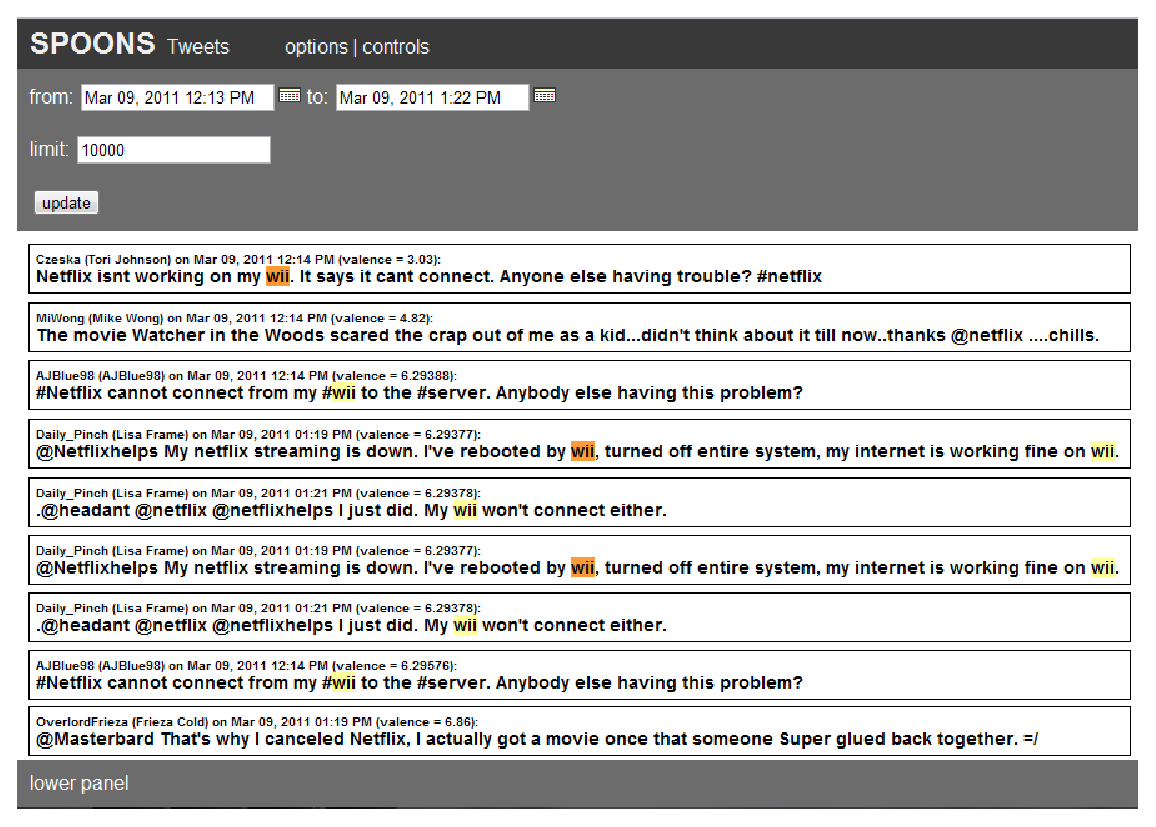
\includegraphics[width=140mm]{images/tweetexample.eps}
      \captionfonts
      \caption[Outage Tweets Example]{Tweets posted on March 9, 2011 during a disruption of Netflix
                                       streaming to the Nintendo Wii console.}
      \label{fig:tweetEx}
   \end{center}
\end{figure}


\chapter{Solution Overview}
\label{overview}

SPOONS (Swift Perception Of Online Negative Situations) is a system that is
designed to use tweets to detect outages in Netflix content delivery systems.
At present, the system supports a wide variety of detection methods that use some combination of time
series analysis, classification, natural language processing, sentiment
analysis, and filtering.

\begin{figure}
   \begin{center}
      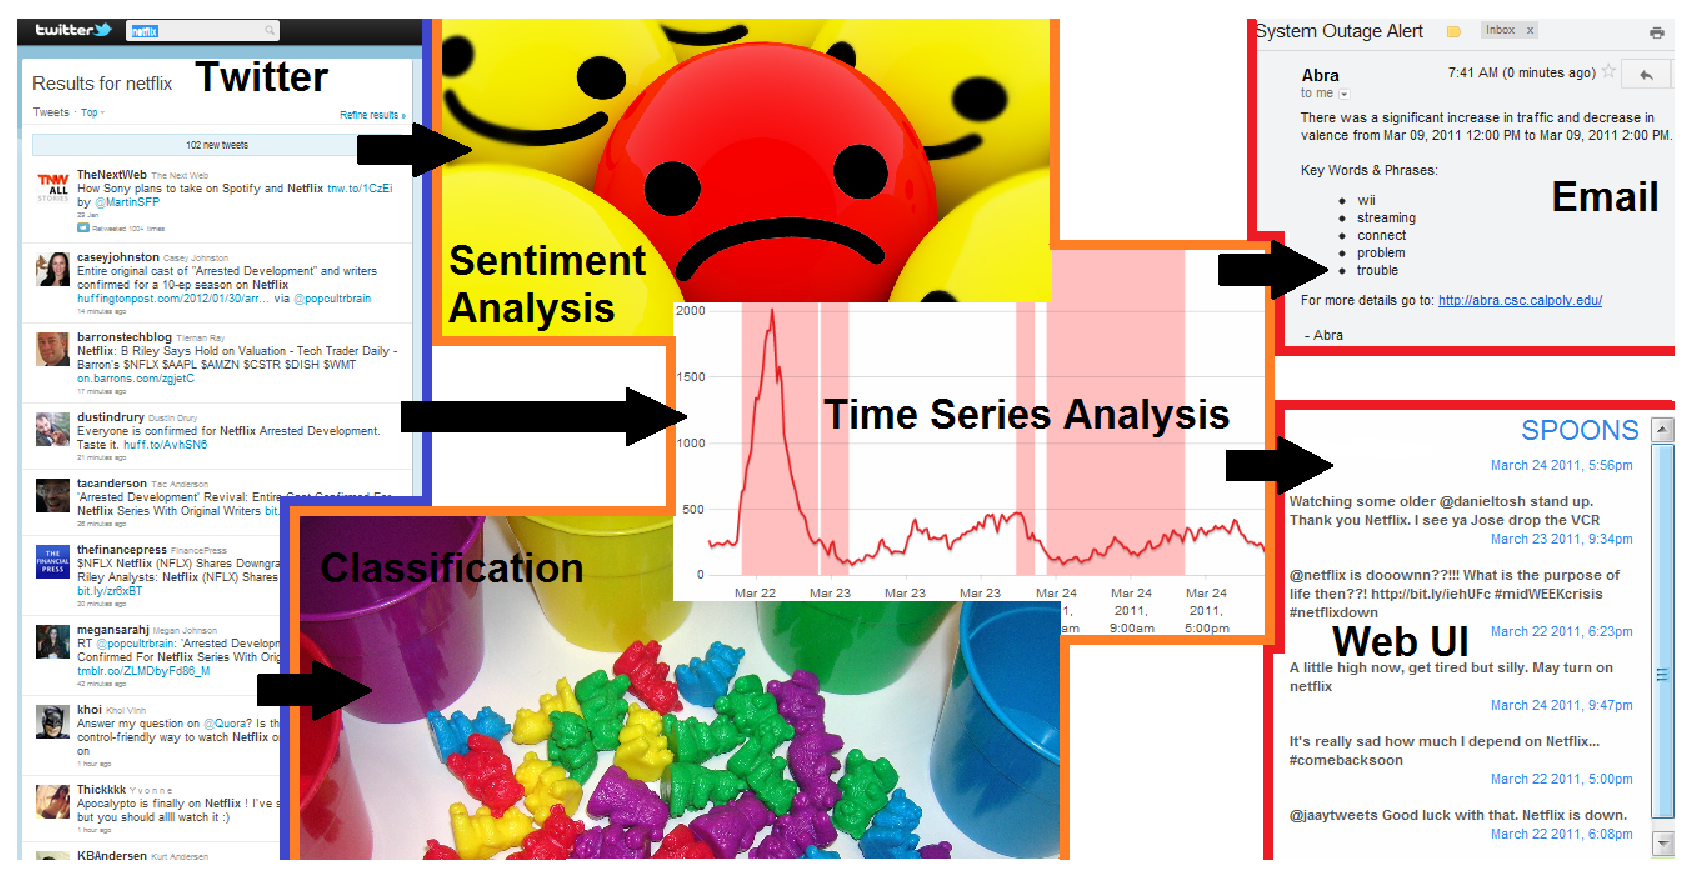
\includegraphics[width=140mm]{images/systemFlow.eps}
      \captionfonts
      \caption[System Concept Diagram]{This system concept diagram shows the general
                                       flow of processing done in the SPOONS system.}
      \label{fig:systemFlow}
   \end{center}
\end{figure}

Figure~\ref{fig:systemFlow} shows how the SPOONS system can be divided into three
main parts: input; analysis pipelines; and output.
The inputs are tweets gathered from Twitter. Then the
analysis pipelines use a combination of sentiment estimation, classification, and
traffic volume analysis to detect when an outage is occurring.
The outputs of the system are: email alerts to Netflix engineers, and a web UI that displays
information about the outage.

\chapter{Ethics of Twitter Observation}

The work in this project uses content that users post on Twitter without their
knowledge. This monitoring system isn't being announced to the
public because widespread knowledge of it would increase the likelihood of a
malicious attack. This practice may lead to concerns about the level of privacy
or ownership being provided to Twitter users regarding the content they post
through the Twitter services. The goal of this section is to address these
concerns by providing more information about the Twitter services and how the
SPOONS system and this work uses the tweets.

\section{Twitter Terms of Service}

According to Twitter Terms of Service\cite{termsOfService} agreement that
everyone accepts automatically by accessing or using Twitter services:

\emph{``You retain your rights to any Content you submit, post or
display on or through the Services. By submitting, posting or displaying Content
on or through the Services, you grant us a worldwide, non-exclusive,
royalty-free license (with the right to sublicense) to use, copy, reproduce,
process, adapt, modify, publish, transmit, display and distribute such Content
in any and all media or distribution methods (now known or later developed).''}

\emph{``This license is you authorizing us to make your Tweets available to the
rest of the world and to let others do the same.''}

\emph{``You agree that this license includes the right for Twitter to make such
Content available to other companies, organizations or individuals who partner with
Twitter for the syndication, broadcast, distribution or publication of such
Content on other media and services, subject to our terms and conditions for
such Content use.''}

\emph{``We encourage and permit broad reuse of Content. The Twitter API exists to
enable this.''}

\emph{``Such additional uses by Twitter, or other companies, organizations or
individuals who partner with Twitter, may be made with no compensation paid to
you with respect to the Content that you submit, post, transmit or otherwise
make available through the Services.''}

In short, Twitter takes ownership of user tweets as soon as they are posted on Twitter.
Using the Twitter API allows SPOONS to obtain the tweets with the consent of Twitter.
Therefore, the collection and analysis of Twitter data by SPOONS is well withing the
Twitter Terms of Service.

\chapter{SPOONS Requirements}
Netflix has provided the following set of key requirements to be met by the
SPOONS system:

\paragraph{Structural Independence.}
The outage detection system shall be structurally independent of both the
software and the hardware infrastructure used by Netflix. It shall rely only on
information that is publicly available and free for use. This ensures that the
outage detection system stays up even when any or all Netflix servers are
experiencing downtime.

\paragraph{Use of Amazon Web Services.}
Netflix is one of the largest customers of Amazon.com's cloud computing
service, Amazon Web Services (AWS). AWS allows users to create new cloud
machines (instances) in many regions throughout the world. The outage
detection system shall be deployed on one or more AWS servers that are
operationally independent of other AWS servers used by Netflix. Using a cloud
solution allows the outage detection and alert system to be deployable on a
global scale.

\paragraph{Real-Time.}
Netflix's streaming services run in real-time and any downtime has an immediate
impact on customers. To minimize that impact, the outage detection system shall notify
Netflix of detected outages as soon as possible.

\paragraph{Precise Outage Detection.}
The number of non-outage situations that raise an alert shall be minimized.
While a small number of false positives detected in real-time may be acceptable,
the outage detection system shall detect outages and generate alerts with as
high precision as possible.

\paragraph{Comprehensive Outage Detection.}
Not all Netflix service outages generate a signal on Twitter. Those that don't may
be allowed to go unnoticed by the outage detection system (as the system
has no basis for detecting them), but any outage that causes a signal on
Twitter shall be detected.

\paragraph{User-Friendly Online UI.}
The outage detection and alert system shall have an easy-to-use, informative,
online UI which shall provide Netflix employees with real-time information and
historic data about the state of Netflix according to Twitter. The information
provided shall include:

\begin{itemize}
   \item times of outages;
   \item times of other anomalous events;
   \item current and recent Netflix-related Twitter traffic trends;
   \item and samples of Netflix-related tweets.
\end{itemize}

\chapter{Contributions and Organization}
\label{contributions-organization}

SPOONS is a continual team effort and has been touched and improved by many different people.
The idea originated at Netflix and was passed to the ABRA team at Cal Poly.
The ABRA team has published a paper on SPOONS \cite{abraPaper}.
In addition, Cailin Cushing defended a thesis on a part of SPOONS devoted to outage detection through sentiment analysis\cite{cailinThesis}.

The main contributions of this work are as follows:

\begin{itemize}
   \item Design and implementation of the SPOONS system.
   \item Design and implementation of the SPOONS framework.
   \item Design and implementation of the SPOONS server architecture.
   \item Design and implementation of the SPOONS distributed computation model.
   \item Design of the SPOONS database structure and all table schemas.
   \item Design and implementation of all SPOONS classification based outage detection methods.
\end{itemize}

The rest of the paper is organized as follows.
Chapter~\ref{background-related-work} covers background and related work.
Part~\ref{arch} discusses the architecture of SPOONS.
Part~\ref{analysis} discuss the work done by the spoons system to detect outages.
With Chapter~\ref{classifiers} focusing on the details of the classifiers used in SPOONS, and
Chapter~\ref{outage-detection} extending the problem of classification to full outage detection.
Part~\ref{conclusions} wraps up the paper.

\chapter{Background \& Related Work}
\label{background-related-work}

%\chapter{Text Stream Analysis}
%\label{background-text-stream}
%Text Stream Analysis \cite{Bansal}\cite{Grinev}\cite{Huang}.

\section{Twitter Traffic Analysis}
\label{background-twitter}
Twitter proves to be a great resource for data mining because of the large number of real-time, posts from millions of users.
However, tweets can be very difficult to work with because they suffer from three large drawbacks:

\paragraph{Length.}
Tweets can only be 140 characters long. This limit severely restricts the possible information content of a tweet.
Compared to more traditional media sources, e.g. news articles, the text of tweets contain almost no information.
Although this makes it very difficult to do naive text classification on tweets, Twitter users have found ways to increase their information density.
Links to news stories, slang, and Twitter symbols (see Section~\ref{class-filter-twitter-symbols}) help Twitter users express more with fewer characters.

\paragraph{Informal Language.}
Informal language, e.g. slang, jargon, and abbreviations, is common place on Twitter.
The use of informal language can be partially attributed to the strict character limit.
Informal language can be difficult to deal with because it it less likely to appear in well established
Natural Language Processing corpora. Not having a corpus forces researchers to either only use unsupervised methods, or
build their own corpus.

\paragraph{Typos.}
The nature of Twitter is very informal for most users whose tweets are only read by their friends.
This informal environment and the large amount of tweets coming from hand-held devices without a traditional keyboard leads to many tweets containing typos.
Typos make text analysis difficult because it obfuscates words and increases the number of unique words.

\subsection{Twitter Classification}
\label{background-twitter-classification}
There has been much work in using classifiers on both tweets and Twitter users.
Most of the classification efforts has gone into trying to determine the sentiment,
the general feeling, of a tweet \cite{Jiang}\cite{Mukherjee}\cite{Saif}\cite{Wang}.
Raz et al. tackle the task of classifying humorous tweets as a specific type of humor
such as irony, observational, or wordplay\cite{Raz}.
The traditional text classification task of topic modeling has also been attempted various times\cite{hong}\cite{Zhao}.
Instead of trying to classify tweets, Pennacchiotti et al. try to classify user associations from
their tweets\cite{Pennacchiotti}.

\subsection{Twitter Anomaly Detection}
\label{background-twitter-anomaly}
TODO(eriq): levchenko

\section{Classifiers}
\label{background-classifiers}
SPOONS uses a variety of different classifiers for text classification.
This section gives an overview of each different type of classifier used.

\subsubsection{Formal Definition}
\label{background-classifiers-def}
The classification problem that the classifiers are trying to solve can be defined as follows:

Given a set of documents $D$
\begin{equation*}
   D = \left \{ d | d \in D \right \}
\end{equation*}
where each document $d$ is a vector of $n$ features
\begin{equation*}
   d = (\textrm{f}_{1}, \textrm{f}_{2}, ..., \textrm{f}_{n})
\end{equation*}
and a set of classes $C$ where
\begin{equation*}
   C = \left \{ c | c \in C \right \}
\end{equation*}
We want to associate each document with a class based off the patterns observed in a training set $T$ of already classified documents.
\begin{equation*}
   T = \left \{ (d, c) | c \in C \right \}
\end{equation*}

\subsection{Naive Bayes}
\label{background-classifiers-naive-bayes}
Naive Bayes classifier works by applying the Bayes' theorem with the assumption that
the probability of each feature in a document is independent from the probability of
any other feature appearing in the same document.\cite{Kibriya}\cite{Frank}

The Bayes' theorem states that the probability of observing class $c$ given document $d$, $Pr(c|d)$, can be represented as:

\begin{equation}
   Pr(c|d) = \frac{Pr(c) \cdot Pr(d|c)}{Pr(d)}
\end{equation}

$Pr(c)$ is the \textsf{prior probability} of class $c$, that is, the probability of
observing $c$ regardless of the document attached to it. When training the classifier, this
is just the percentage of times that the class appeared in the training set.

$Pr(d)$ is the \textsf{prior probability} of document $d$. Like $Pr(c)$, it is just the
probability of observing the collection of features $d$ regardless of the class associated with it.
Note that for classification, it is not necessary to compute $Pr(d)$ because it is constant among all
documents and classes. A classifier can just choose the class with the largest $Pr(c) \cdot Pr(d|c)$ term.

$Pr(d|c)$ is the probability of observing document $d$ given that $d$ is already recognized as belonging to
class $c$. Remember that document $d$ is really just a vector of $n$ features, $(\textrm{f}_{1}, \textrm{f}_{2}, ..., \textrm{f}_{n})$.
Assuming \textbf{conditional independence} (the \textsf{naive} part in Naive Bayes), $Pr(d|c)$ can be
constructed as a product of the probability of observing each feature in $d$:

\begin{equation}
   Pr(d|c) = Pr(\textrm{f}_{1}|c) \cdot Pr(\textrm{f}_{2}|c) \cdot ... \cdot Pr(\textrm{f}_{n}|c) = \prod_{i = 1}^{n}Pr(\textrm{f}_{i}|c)
\end{equation}

Now the last step is to estimate the conditional probabilities of the $n$ features.
When dealing with discrete features, then estimating $Pr(\textrm{f}_{m}|c)$ ($1 \leq m \leq n$) can be done by
finding the percentage of training documents that contain feature $\textrm{f}_{m}$ and have class $c$.

\subsection{Bayes Net}
\label{background-classifiers-bayes-net}
A Bayesian Network is a probabilistic, directed acyclic graphs that represents a set of random variables and their conditional probabilities.
In a Bayesian Network, the collection of incoming edges represent the conditional probability distribution between two random variables.
Each node represents a variable and a probability function that takes as input the state of the node's parents.\cite{Pearl}\cite{Neapolitan}

Figure~\ref{fig:bayesNet1} shows a simple Bayesian Network that models the chance of going on a picnic.
Note that whether or not it is Spring affects the chance of it raining; and both the season and weather
affect the chance of going on a picnic.

Figure~\ref{fig:bayesNet2} shows the probability distributions for the network. The chance of the season being Spring if
fully independent, and therefore takes no parameters into its probability function. However, the weather and picnic decision
takes one and two input parameters respectively.

\begin{figure}
   \begin{center}
      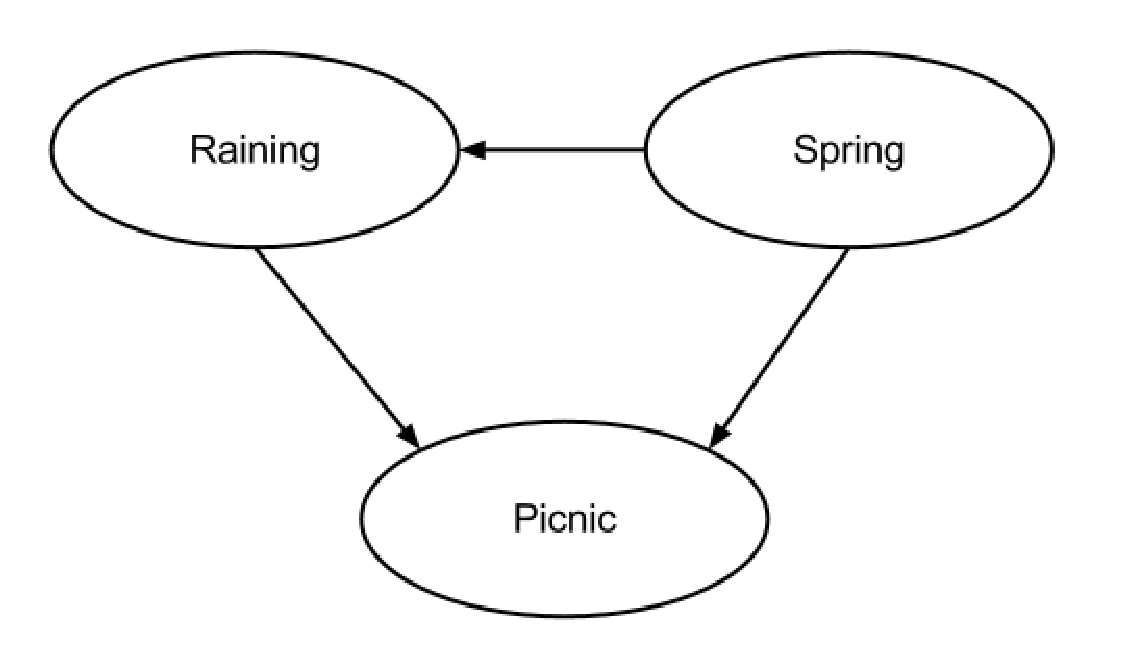
\includegraphics[width=0.4\textwidth]{images/Bayes_Net_1.eps}
      \captionfonts
      \caption[Simple Bayes Net]{A simple Bayesian Network modeling the chance of going on a picnic given the season and weather. The season affects the weather and both the season and weather affect the chance of going on a picnic.}
      \label{fig:bayesNet1}
   \end{center}
\end{figure}

\begin{figure}
   \begin{center}
      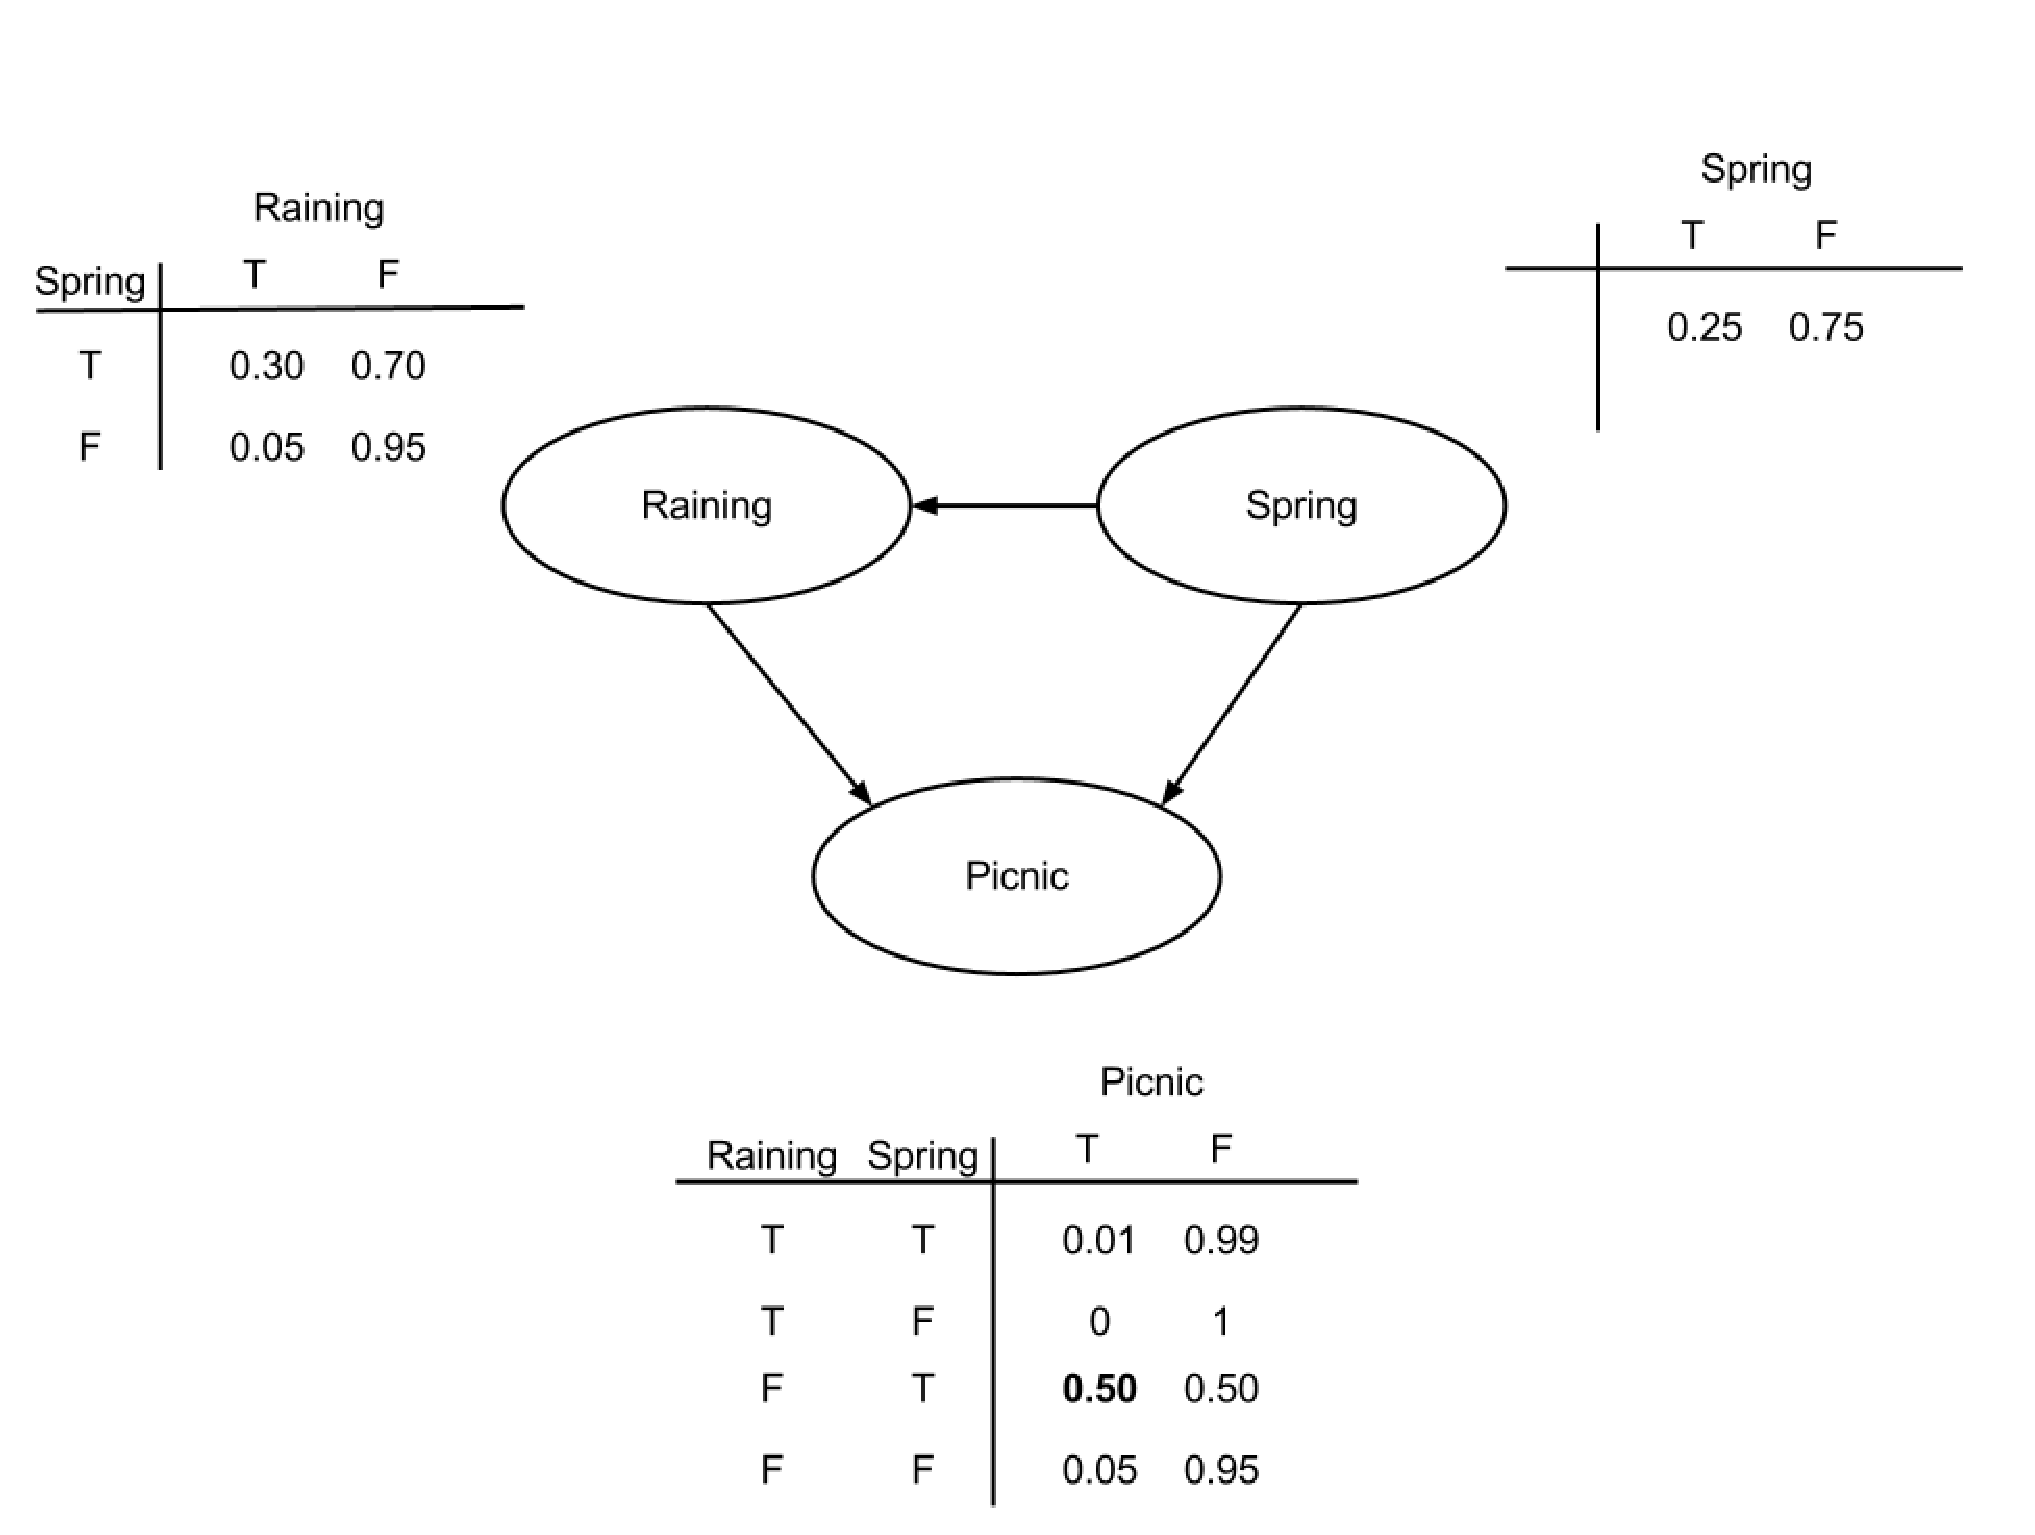
\includegraphics[width=0.8\textwidth]{images/Bayes_Net_2.eps}
      \captionfonts
      \caption[Bayes Net With Probabilities]{The simple Bayesian Network augmented with the probability functions for each node.}
      \label{fig:bayesNet2}
   \end{center}
\end{figure}

\subsection{J48}
\label{background-classifiers-j48}
J48 is a specific implementation of the C4.5 algorithm.
C4.5 is an algorithm that is used to generate a decision tree given a training set.

\subsubsection{Decision Trees}
\label{background-classifiers-j48-decision-trees}
A decision tree is a simple data structure used to come to come conclusion based off of a number of observations.
At each non-terminal node, a question is asked. The answers to the question are represented by the node's outgoing edges.
The tree is traversed in this fashion until a terminal node is reached. The terminal node contains the final conclusion.
In a classification context, each non-terminal node is labeled with an attribute, each edge is the value (or range of values)
for that attribute, and each terminal node is a class. Each attribute can only appear once in the tree.

\begin{figure}
   \begin{center}
      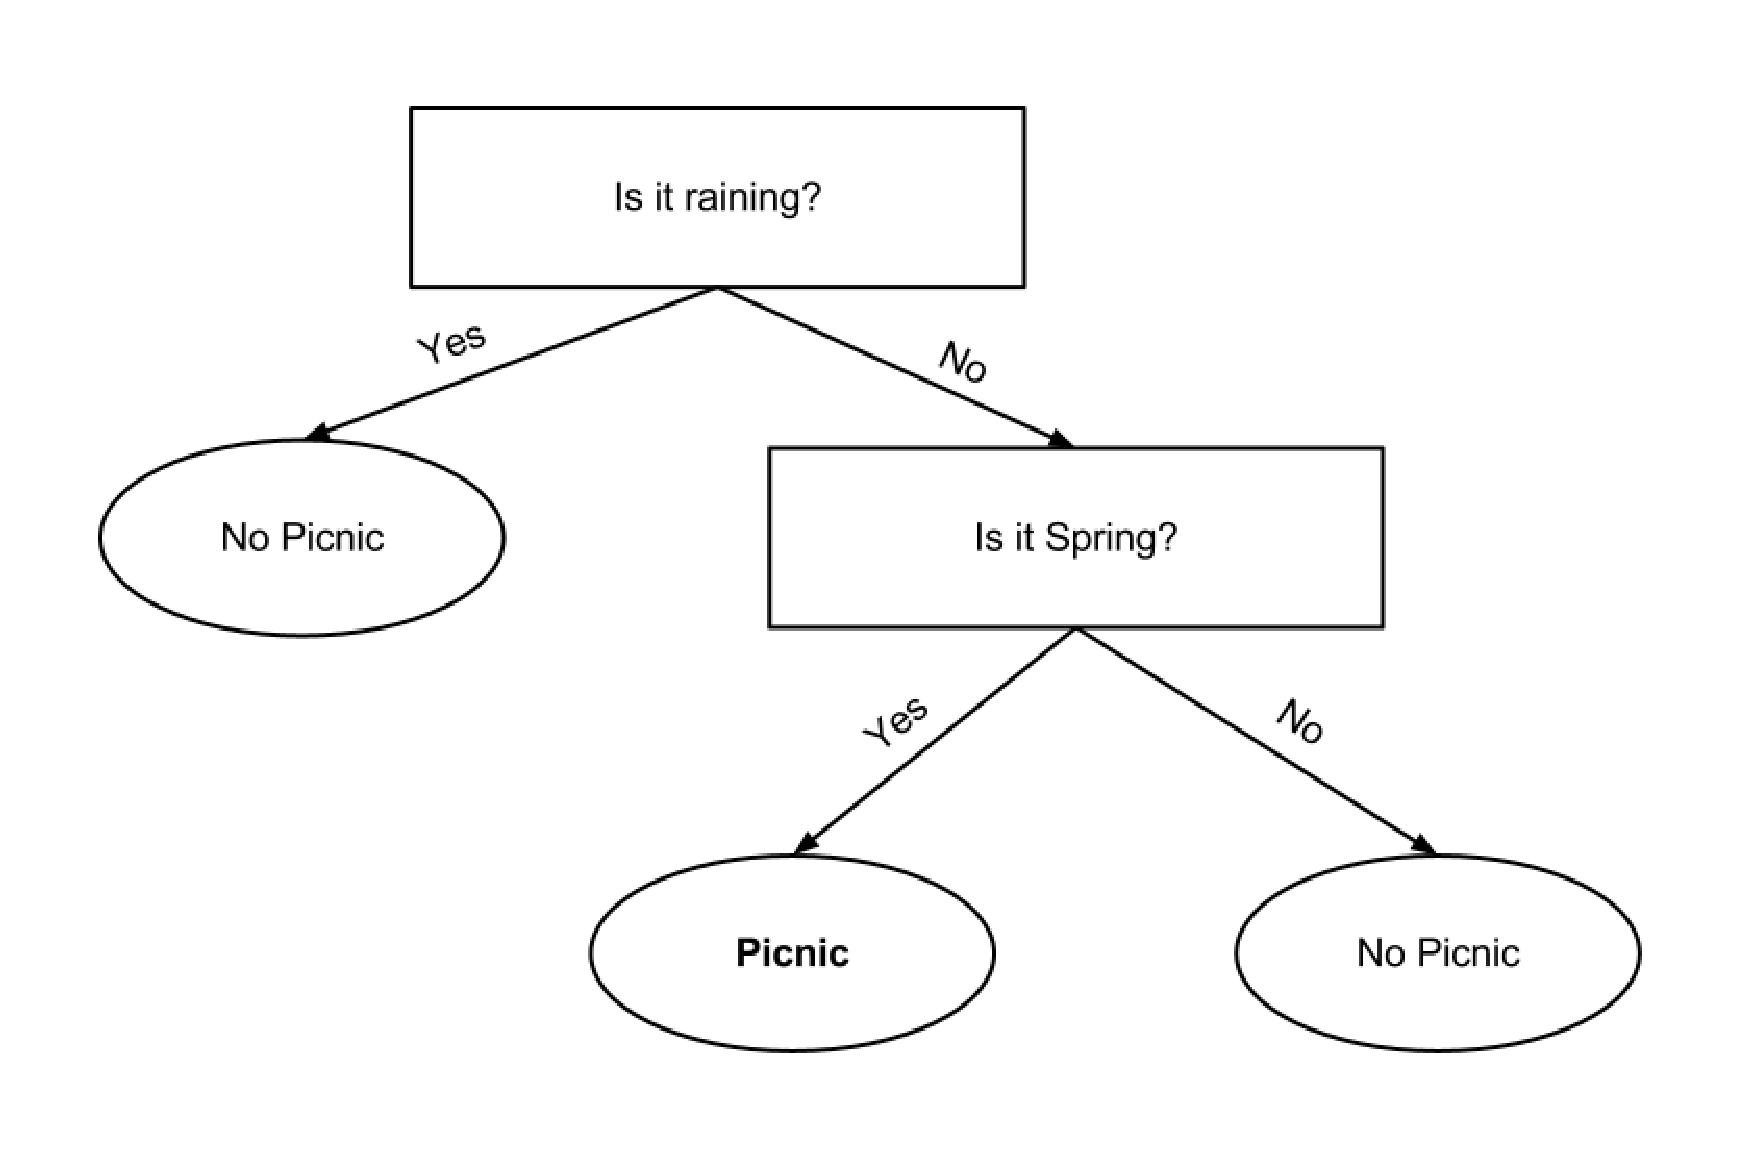
\includegraphics[width=0.8\textwidth]{images/Decision_Tree.eps}
      \captionfonts
      \caption[Simple Decision Tree]{A simple decision tree trying to answer the question of whether or not to go on a picnic.}
      \label{fig:decisionTree}
   \end{center}
\end{figure}

Figure~\ref{fig:decisionTree} shows a decision tree that may be generated for the picnic example discussed in Section~\ref{background-classifiers-bayes-net}.
Note that once the decision tree is built, reaching a terminal node is fairly trivial.

\subsubsection{C4.5 --- Decision Tree Induction Algorithm}
\label{background-classifiers-j48-c45}
C4.5 recursively builds a decision tree by continually splitting the dataset on a single attribute\cite{Quinlan}.
The splitting attribute is determined by the normalized information gain (Kullback-Leibler divergence) and becomes a
node in the tree and the possible values for the attribute become edges. Each subtree is then recursively built using only the
data where the splitting attribute takes the value given by the incoming edge. The algorithm has two stopping conditions.
First, when all the data has the same class. In which case a single node tree is constructed that contains the class.
Secondly, when there are no more attributes or when the information gain from splitting on each attribute is below a threshold.
In this case, a single node tree is constructed which contains the plurality class.

\subsection{K-Nearest Neighbors}
\label{background-classifiers-knn}
$k$-Nearest Neighbors (KNN) is simple and effective classification technique\cite{Duda}.
While training, the classifier remembers the entire training set.
During the classification phase, the classifier finds the $k$ nearest neighbors
to the query point. The predicted class is simply the plurality of the $k$ nearest neighbors.
Figure~\ref{fig:knn} shows an example of $k$-Nearest Neighbors with a simple search space.

\begin{figure}
   \begin{center}
      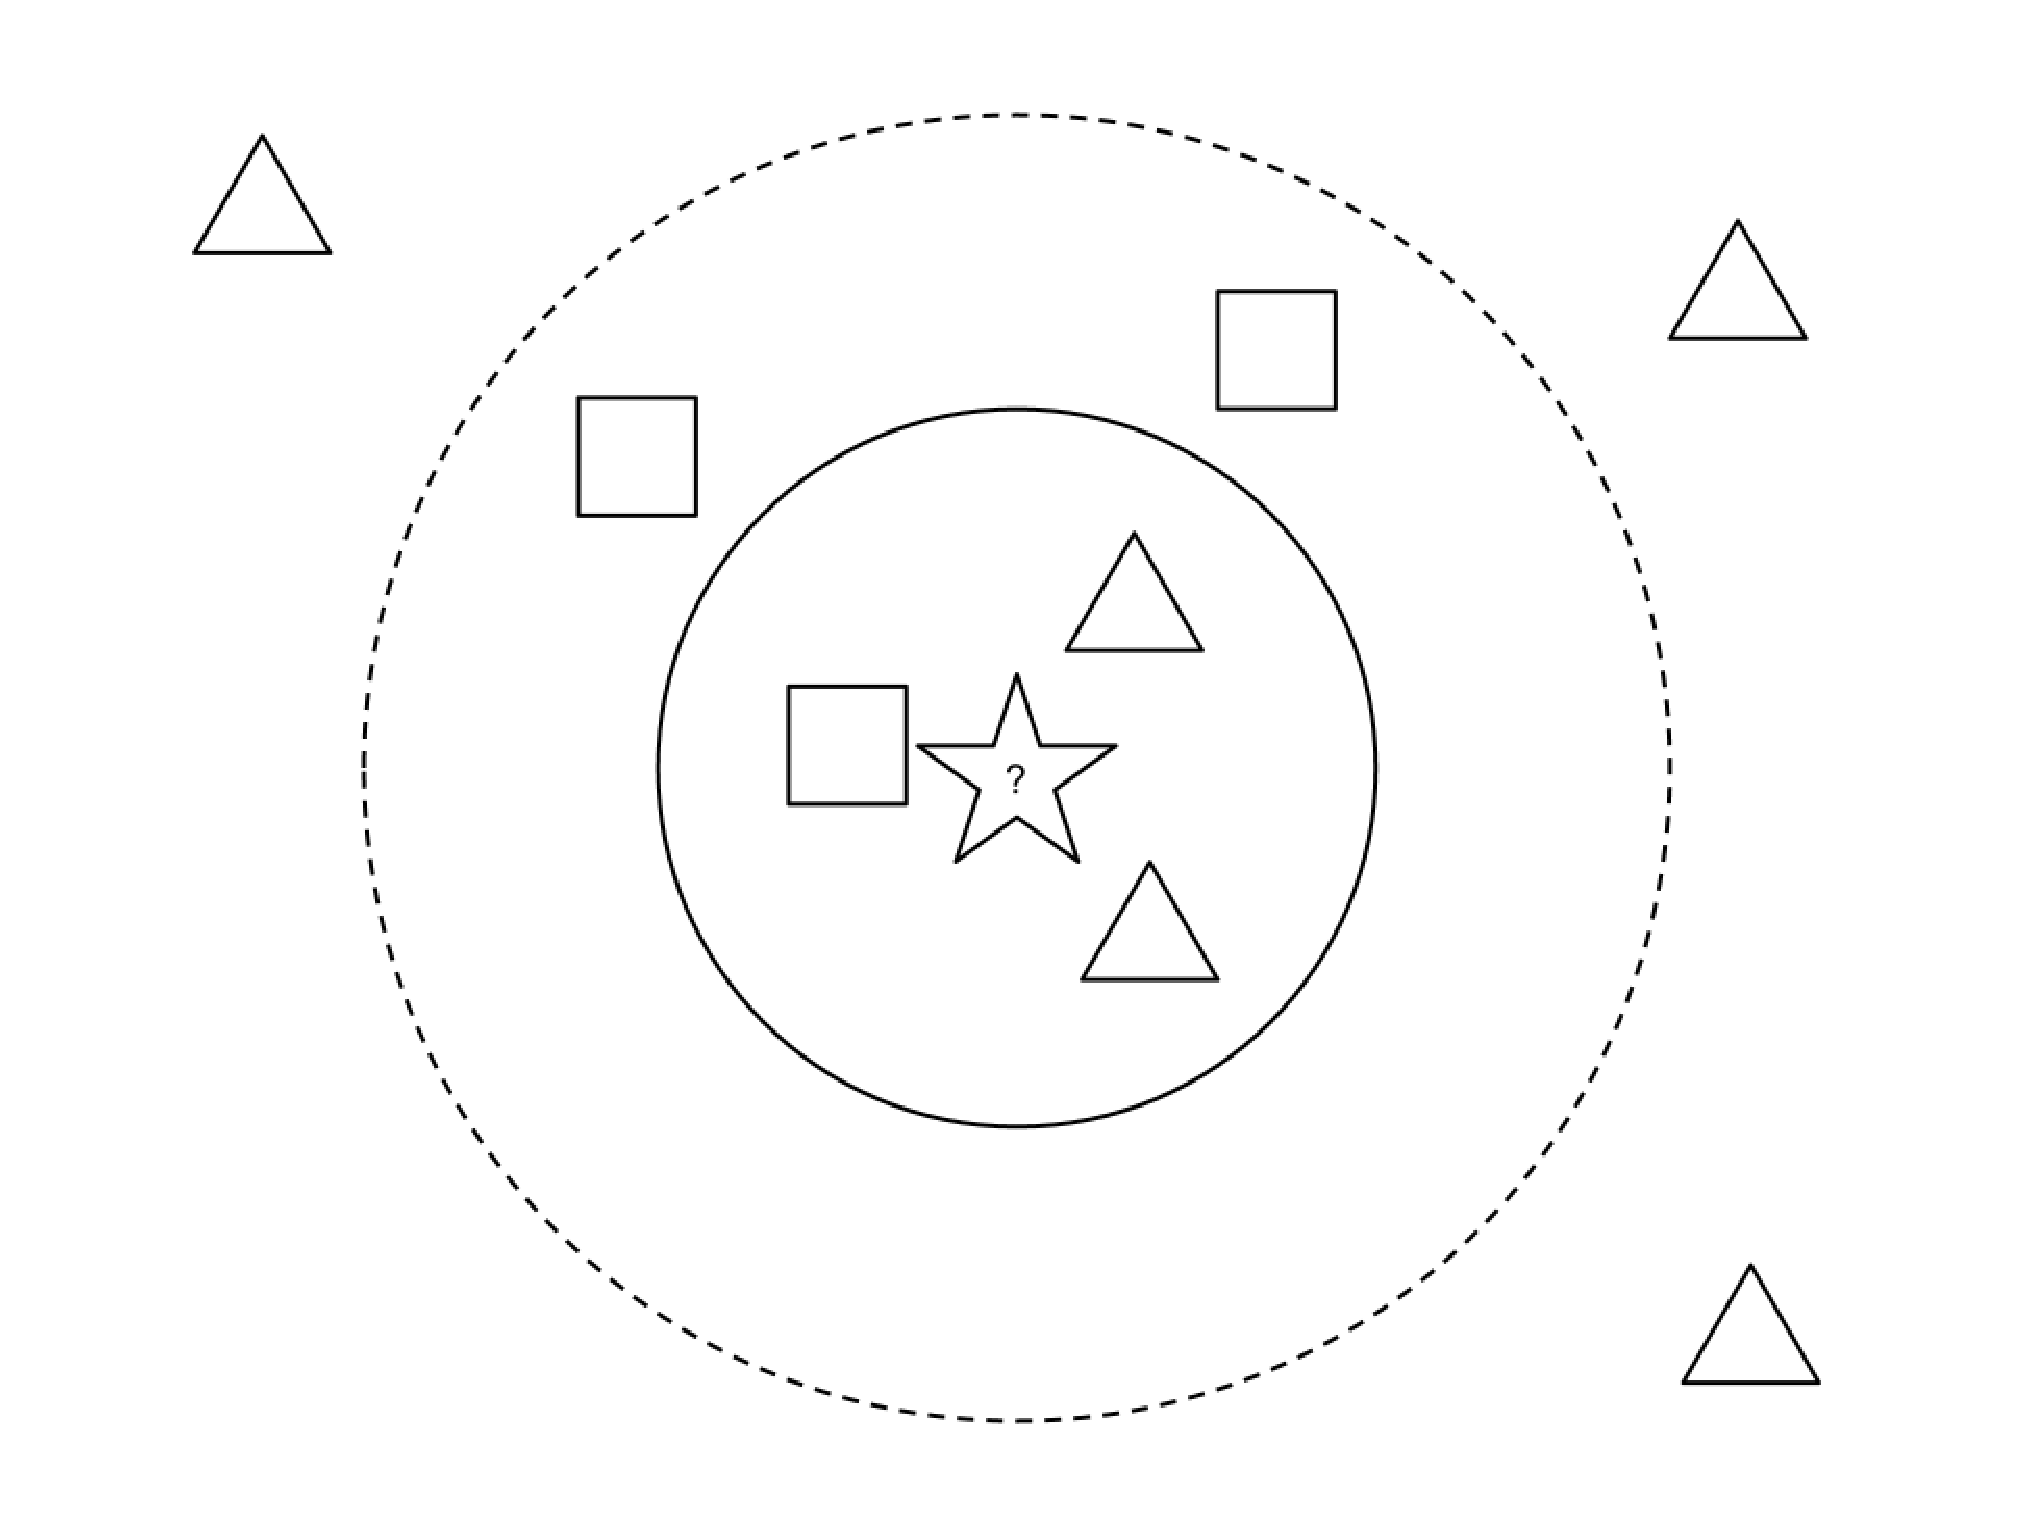
\includegraphics[width=0.4\textwidth]{images/KNN.eps}
      \captionfonts
      \caption[K-Nearest Neighbors]{A simple example of KNN. If $k = 3$, then the query point (the star) will be classified as a triangle. However, if $k = 5$ then the query point will be classified as a square.}
      \label{fig:knn}
   \end{center}
\end{figure}

\subsection{Support Vector Machines}
\label{background-classifiers-svm}
Support Vector Machines (SVMs) are considered one of the best off-the-shelf classification techniques\cite{Vapnik}.
When training, SVMs use hyperplanes to partition the data into surfaces based off of the different classes of the training examples.
When classifying, the SVM finds which surface the query point falls on and give that class to the point.
SVMs try and choose the partitioning hyperplane to maximize the margin between the two groups of data.
Depending on the implementation, the SVM may choose the optimal partition or just an approximation.

\begin{figure}
   \begin{center}
      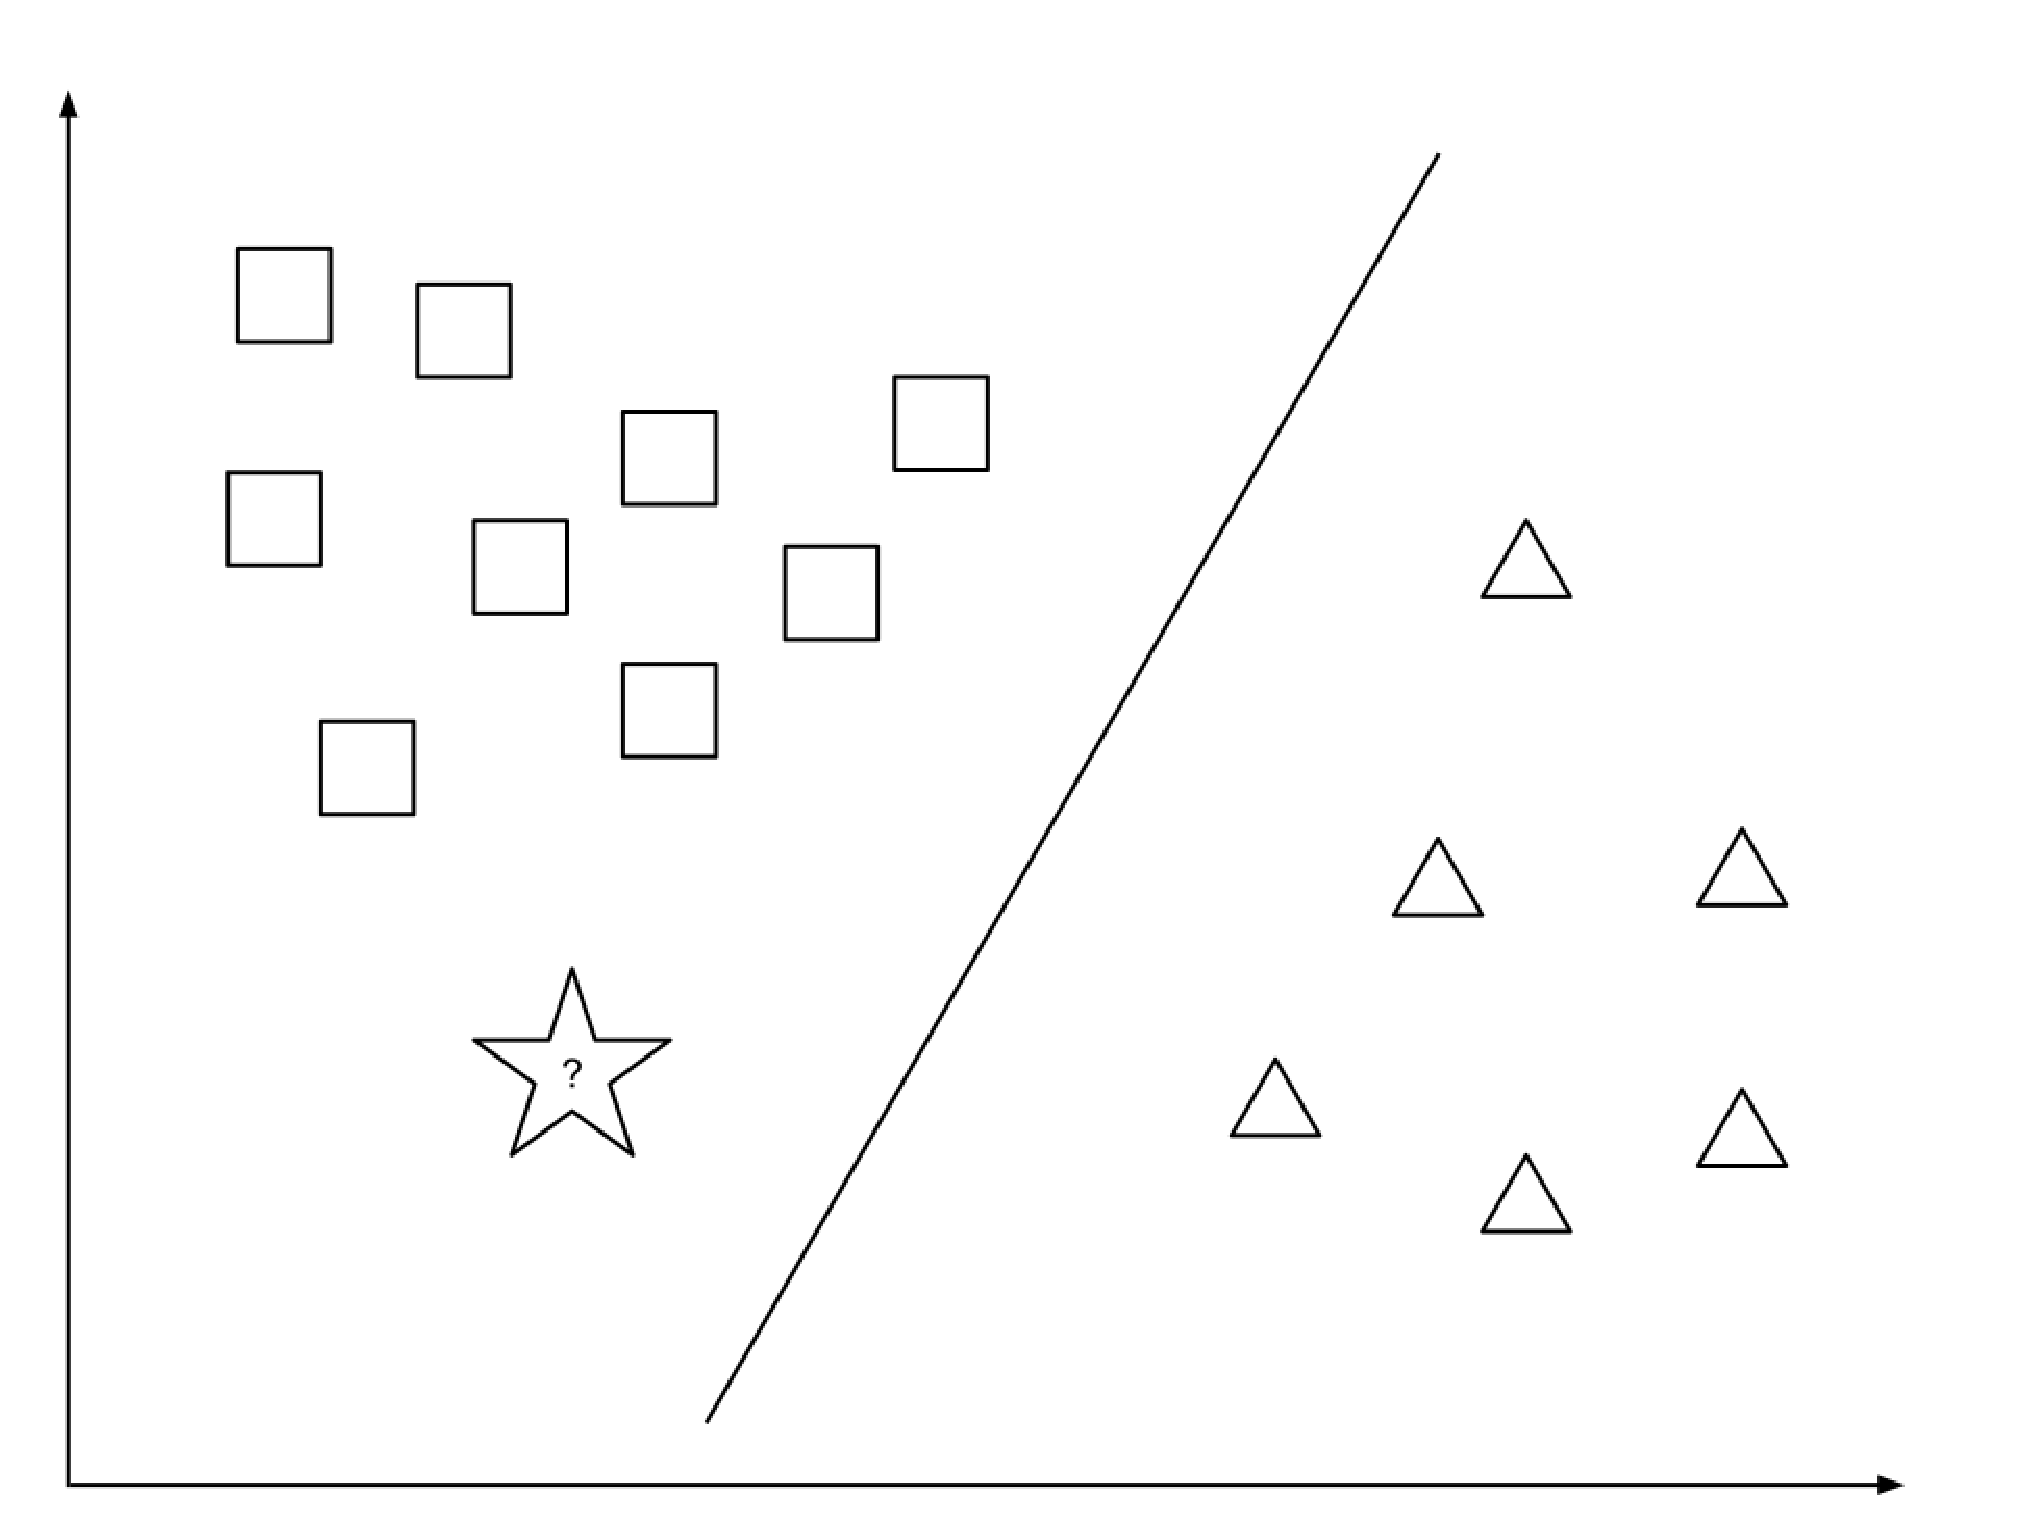
\includegraphics[width=0.4\textwidth]{images/SVM.eps}
      \captionfonts
      \caption[Support Vector Machine]{A simple example of a support vector machine. The SVM chose a partition that maximizes the margin between the squares and triangles.}
      \label{fig:svm}
   \end{center}
\end{figure}

Figure~\ref{fig:svm} shows a simple example of a linear binary SVM.
Note that the partition line is chosen to maximize the distance between the triangles and squares.
The query point (the star) falls into the squares' partition and is therefore classified as a square.

\subsubsection{Sequential Minimal Optimization}
\label{background-classifiers-svm-smo}
Sequential Minimal Optimization (SMO) is an efficient algorithm for solving SVMs invented by John Platt in 1998\cite{Platt}.

\subsection{BPNB}
\label{background-classifiers-bpnb}
BPNB is a method developed by Chu\cite{bpnb}.
It is based off of Naive Bayes, except the relative probability of each feature is accounted for.

BPNB states that the probability of observing class $c$ given document $d$, $Pr(c|d)$, can be represented as:

\begin{equation}
   Pr(c|d) = Pr(c) \cdot \prod_{i = 1}^{n}g(\textrm{f}_{i},c)
\end{equation}

Where $g(\textrm{f}_{m}, c)$ is the weight of feature $\textrm{f}_m$ in class $c$.

\begin{equation}
   g(\textrm{f}_m, c) = \beta^{1 - \frac{Pr(\textrm{f}_m|c)}{Ave(\textrm{f}_m)}}, 0 < \beta < 1
\end{equation}

\begin{equation}
   Ave(\textrm{f}_m) = \frac{\sum_{i=1}^{|C|} Pr(\textrm{f}_m|c_{i})}{|C|}, c_i \in C
\end{equation}

\subsection{WEKA}
\label{background-weka}
SPOONS utilizes several classifiers provided in the \textit{WEKA Machine Learning Package}.
WEKA is an open source package written under the GNU General Public License\cite{weka}.

\section{Singletons}
\label{background-singletons}
The SPOONS architecture makes heavy use of singletons to guarantee certain assumptions.
A \textbf{singleton} is an object-oriented class that may have at most one instance of itself instantiated at a time.
SPOONS uses two types of singletons: singletons that are relative to the base class and singletons that are relative to the
child classes.

\paragraph{Base Relative Singletons.}
Base relative singletons are singletons that only allow one instance of to base class in the inheritance hierarchy to be instantiated
at a time. This means that there can only be one instance allowed for the entire inheritance hierarchy.
Figure~\ref{fig:baseSingleton} shows an inheritance diagram of a hierarchy that uses a base relative singleton.
Note that because one of the children have been instantiated, no other class in the hierarchy can be instantiated.

\begin{figure}[H]
   \begin{center}
      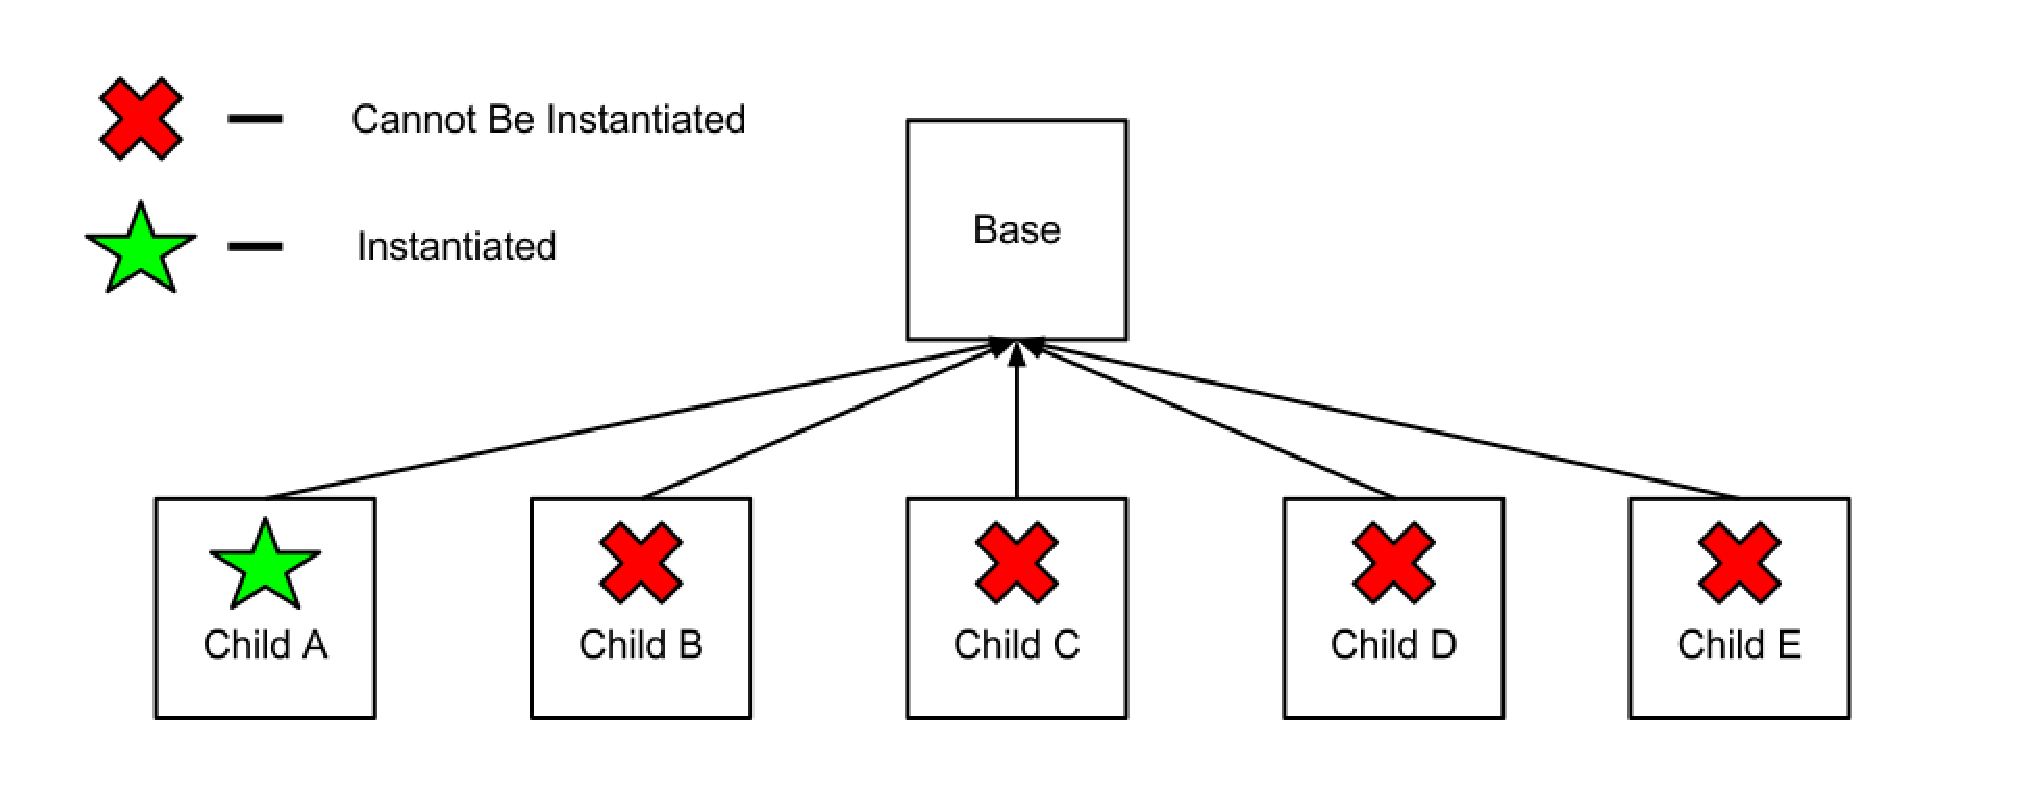
\includegraphics[width=0.6\textwidth]{images/Base_Singleton.eps}
      \captionfonts
      \caption[Base Relative Singleton]{An example base relative singleton inheritance hierarchy. Note that instantiating any child removes the ability to instantiate any other part of the hierarchy.}
      \label{fig:baseSingleton}
   \end{center}
\end{figure}

\paragraph{Child Relative Singletons.}
Child relative singletons are singletons that allows only one instance of each leaf child in the inheritance hierarchy to be instantiated
at a time. This allows the inheritance hierarchy to have as many instance as leaf children.
Figure~\ref{fig:childSingleton} shows an inheritance diagram of a hierarchy that uses child relative singletons.
Note that all the children can be instantiated once.

\begin{figure}[H]
   \begin{center}
      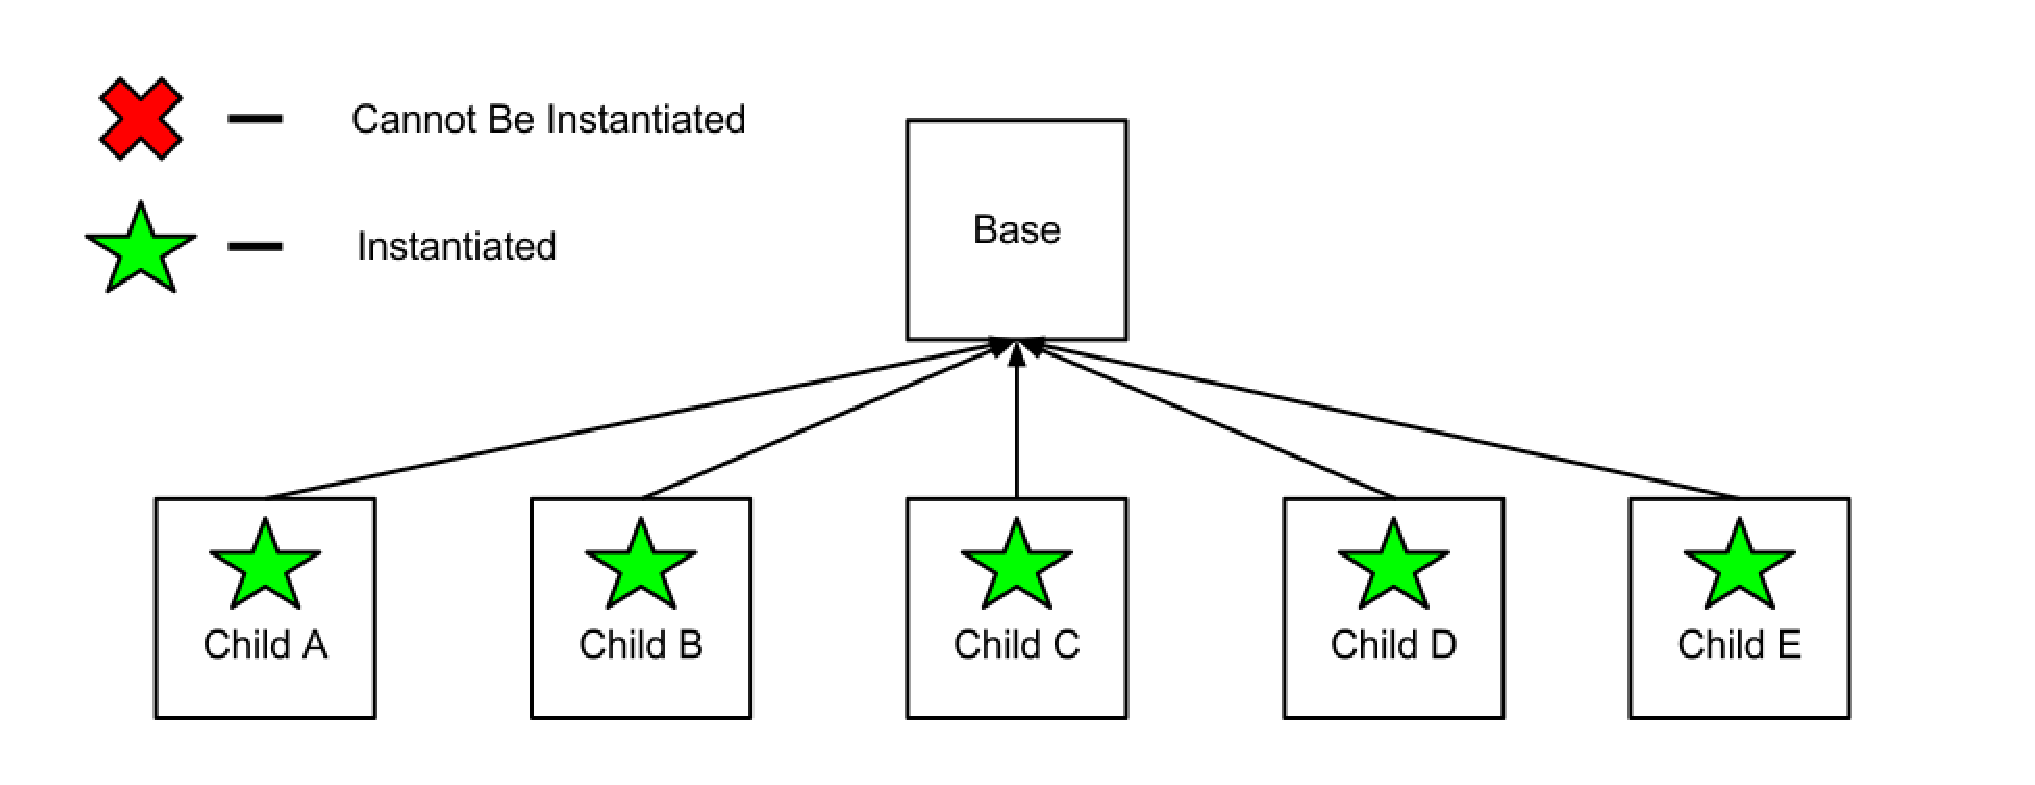
\includegraphics[width=0.6\textwidth]{images/Child_Singleton.eps}
      \captionfonts
      \caption[Child Relative Singleton]{An example child relative singleton inheritance hierarchy. Note that any child can be instantiated, but only once.}
      \label{fig:childSingleton}
   \end{center}
\end{figure}

\chapter{Twitter API}
\label{api}
All of the data data that SPOONS uses is obtained in real time using the Twitter Search REST API\cite{TwitterAPI}.

\section{Rate Limiting}
\label{api-rate-limit}
Twitter imposes a limit on the number of queries to the Search API. Twitter does not publish the official
limit. However, our experiments suggest that SPOONS can query the API for all new Tweets once every two minutes without
suffering from rate limiting.

\section{Pagination}
\label{api-pagination}
Twitter paginates the results from its search API. The maximum results you can get per page is 100, and each
query can return at most 15 pages. Therefore when there are more than 1500 tweets generated per minute,
SPOONS must do multiple search queries.

\section{Query Anatomy}
\label{api-anatomy}
The typical structure of a Twitter API query is shown in Figure~\ref{fig:apiQuery}.

\begin{figure}[H]
   \begin{center}
      \fbox{
         \begin{minipage}{12cm}
            \begin{center}
               http://search.twitter.com/search.\textbf{json}?\textbf{q}=$\langle$query$\rangle$\&\textbf{rpp}=100\&\\
               \textbf{result\_type}=recent\&\textbf{since\_id}=$\langle$tweet id$\rangle$\&\textbf{max\_id}=$\langle$tweet id$\rangle$
            \end{center}
         \end{minipage}
      }
      \captionfonts
      \caption[Twitter API Query]{The structure of a typical query to the Twitter API.}
      \label{fig:apiQuery}
   \end{center}
\end{figure}

The parameters are:

\begin{description}

\item[json:]
Twitter can supply the result data in either ATOM or JSON format. Testing with both have shown that the ATOM
results are less consistent and provide less data. Because of the more accurate information returned from the JSON
API, we are able to write more efficient queries. Using the ATOM API, we could query Twitter only once every five
minutes; as opposed to every two minutes with the JSON API.

\item[q:]
The search query. Twitter supports some advanced search features such as conjunction and negation.

\item[rpp:]
``Results Per Page''. Twitter paginates the responses from the Search API. SPOONS always uses the maximum pagination value to decrease the number of requests per hour and lessen the chance of being rate limited.

\item[result\_type:]
Twitter allows users to get results ordered by either relevance or time. Since we want to gather all tweets about
our query, we choose to get the results ordered by time. In addition, the ``since\_id'' and ``max\_id''
parameters do not work when results are sorted by relevance.

\item[since\_id:]
The id of the oldest tweet that should be returned. This is not a hard limit, but provides a nice starting point.

\item[max\_id:]
The id of the most recent tweet that should be returned. It may seem counter-intuitive to provide a cap on the
most recent tweet, when one wants to query for all of the most recent tweets. However when a query's results spans across
more than 15 pages, it needs to be broken into a new query restarting at the first page. In this situation,
not providing an upper limit includes new tweets outside of the original search scope. This can result in tweets that are forever lost to us.

\end{description}

\section{Result Anatomy}
\begin{figure}
   \begin{center}
      \fbox{
         \begin{minipage}{160mm}
            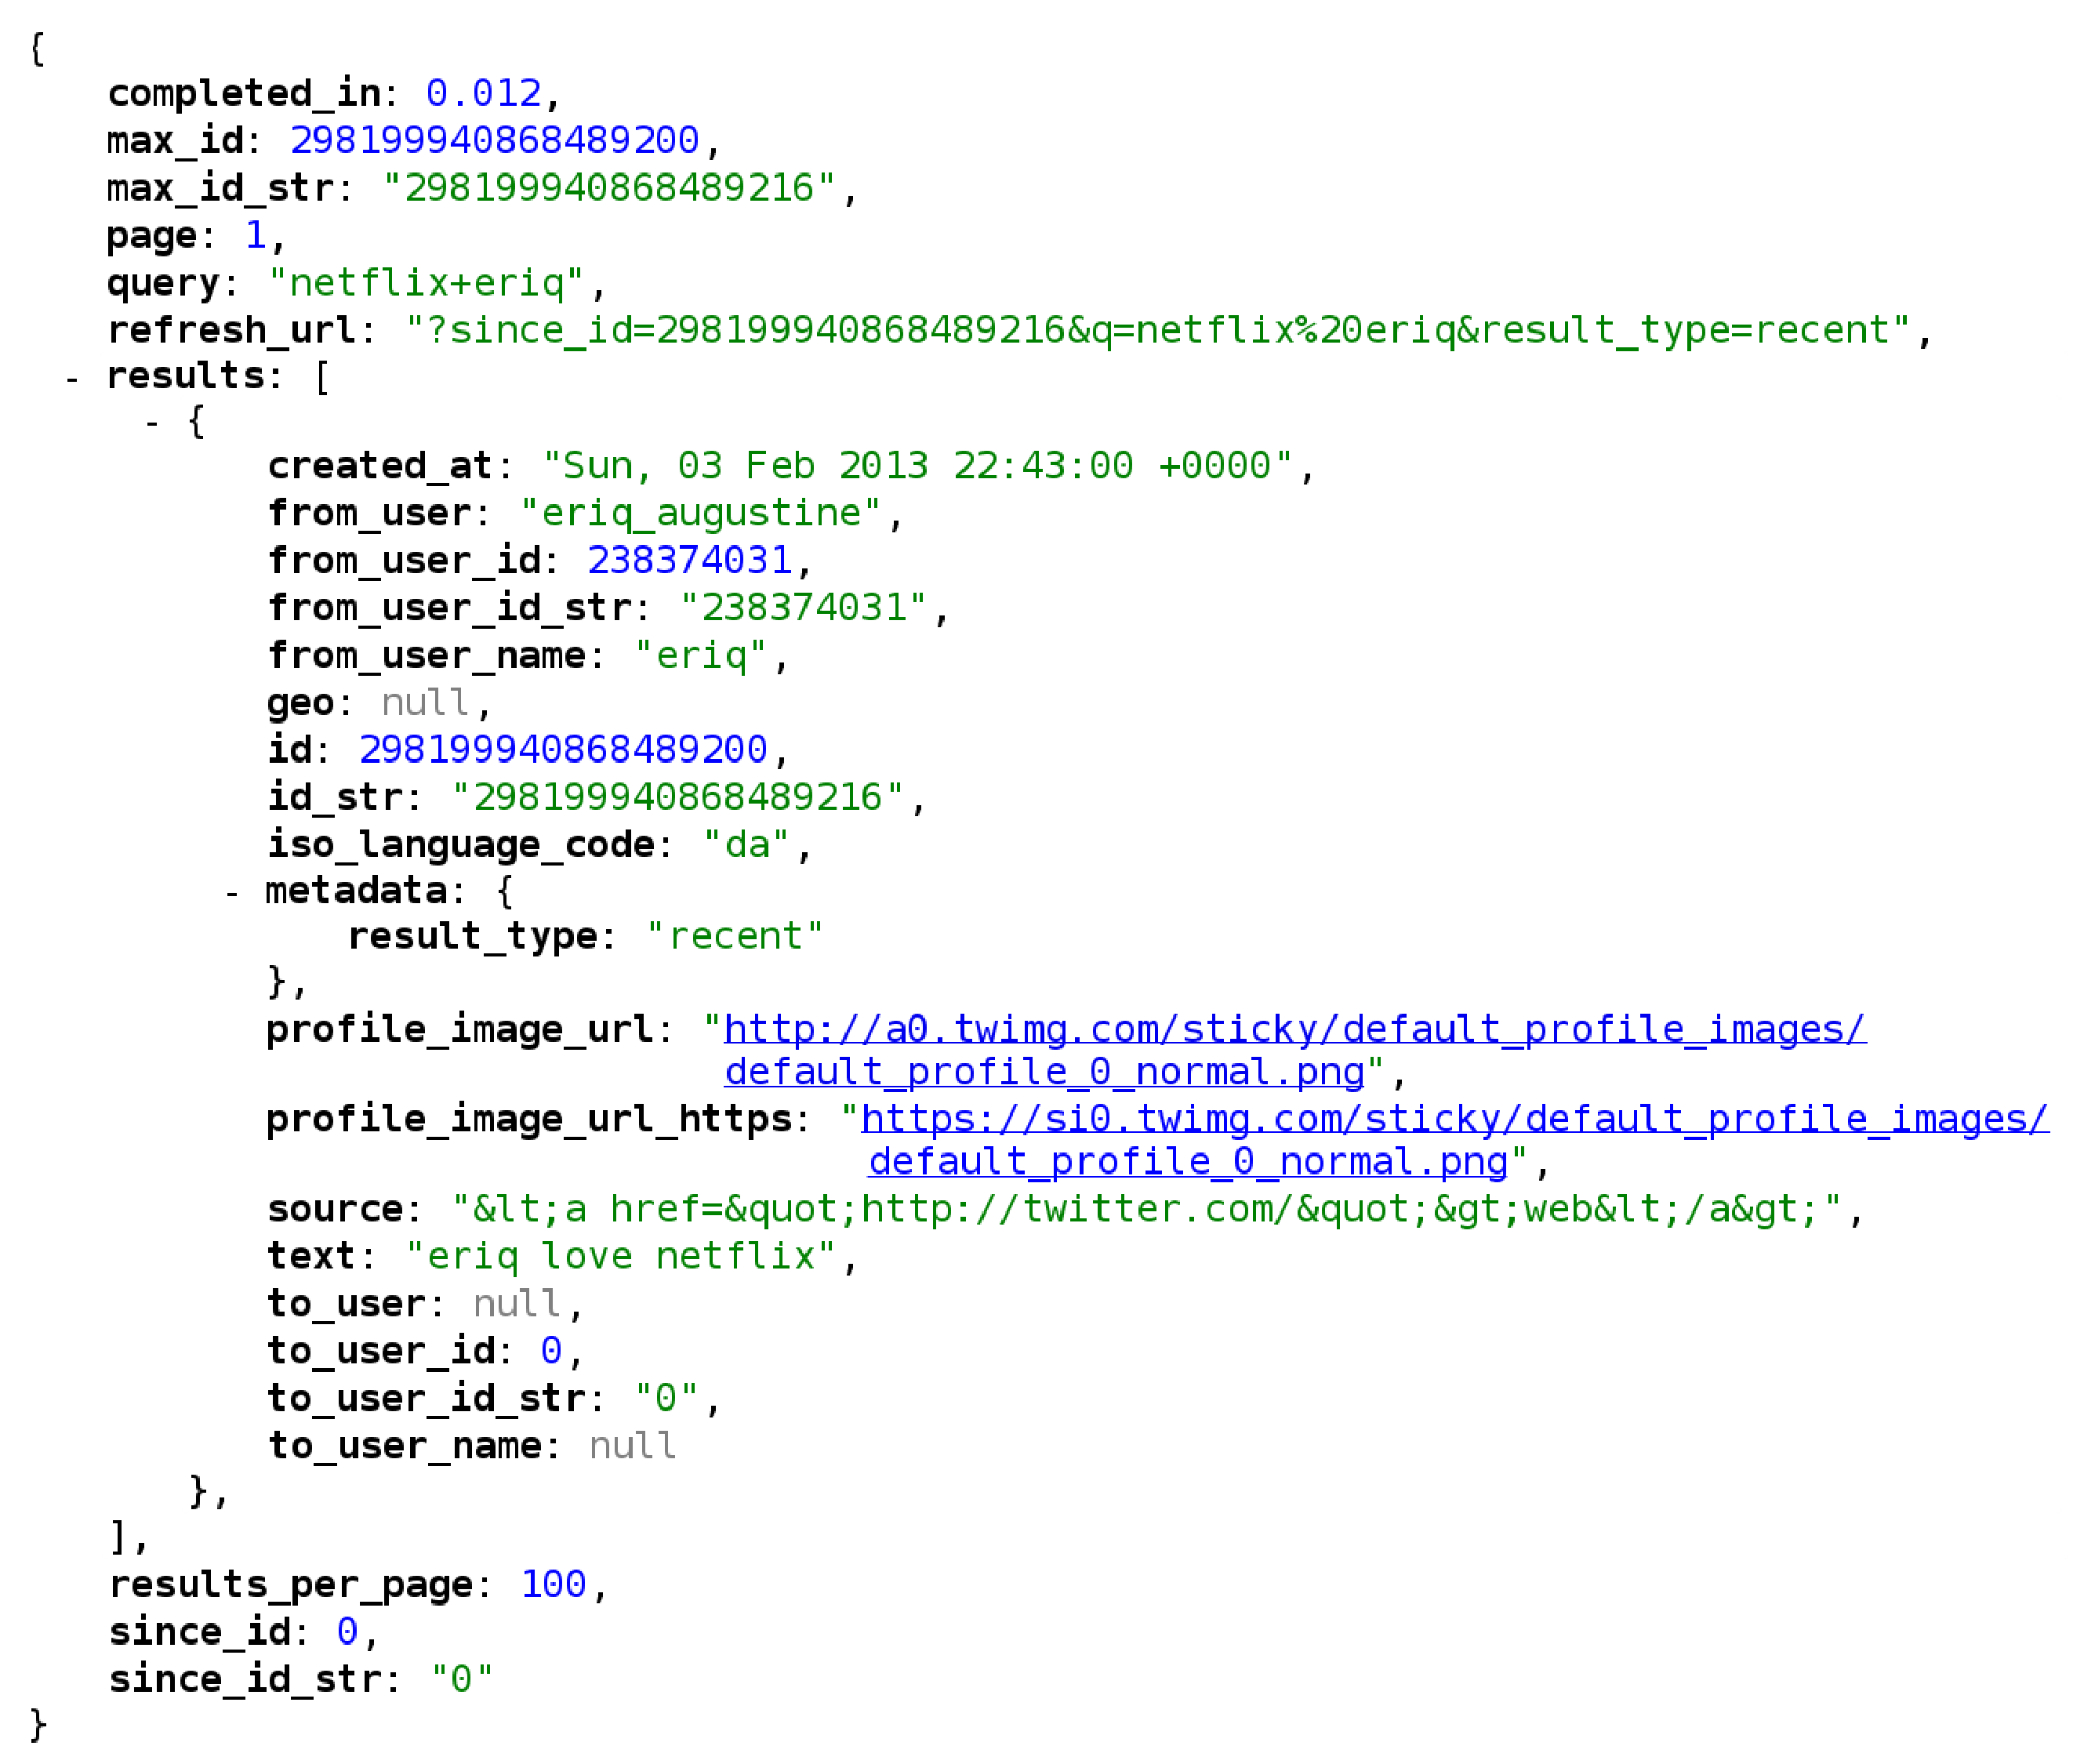
\includegraphics[width=150mm]{images/api_result.eps}
         \end{minipage}
      }
      \captionfonts
      \caption[Twitter Search API Result]{A JSON result from the Twitter Search API}
      \label{fig:apiRes}
   \end{center}
\end{figure}

Figure~\ref{fig:apiRes} shows the result from the query ``eriq netflix''. Notice that some fields,
like the \textsf{geo} field, can be null. Also note that the API incorrectly guessed the language of the tweet as Danish.


%%%%%%%%%%%%%%%%%%  Arch  %%%%%%%%%%%%%%%%%%%%%


\part{SPOONS Architecture}
\label{arch}

\chapter{Architecture Breakdown}
\label{arch-breakdown}

\begin{figure}
   \begin{center}
      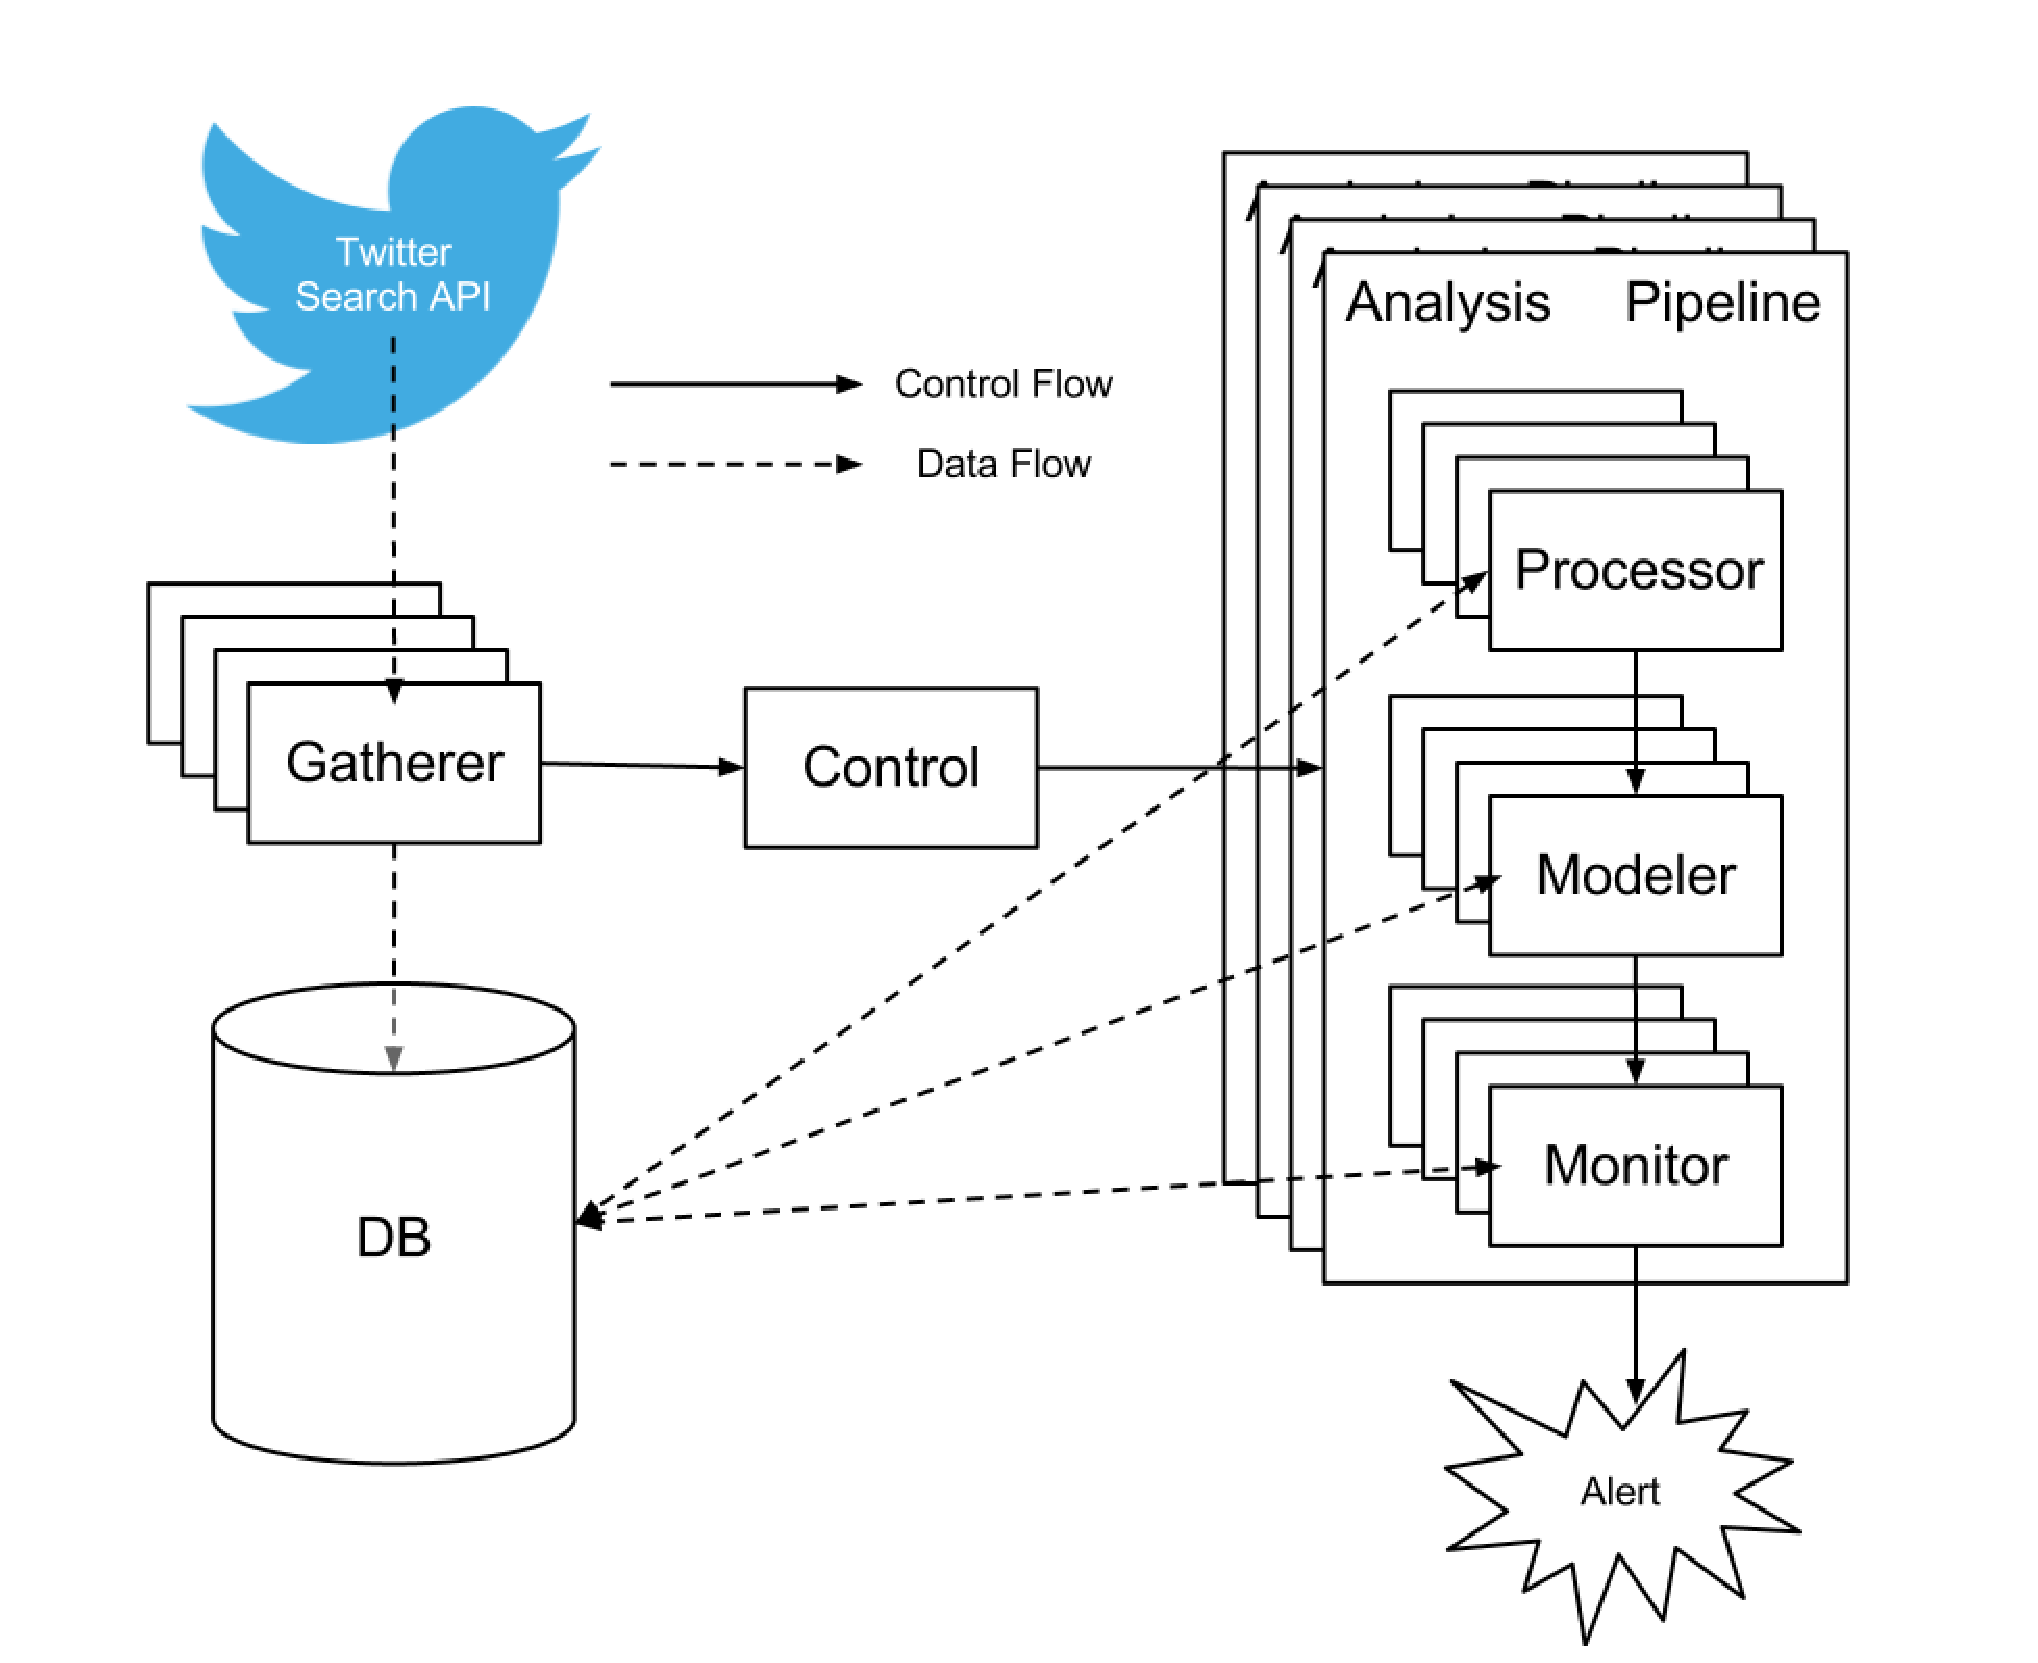
\includegraphics[width=0.8\textwidth]{images/SPOONS_Framework_Architecture.eps}
      \captionfonts
      \caption[SPOONS Framework Architecture]{The flow of control and data through the SPOONS framework system.}
      \label{fig:frameworkArch}
   \end{center}
\end{figure}

\begin{figure}
   \begin{center}
      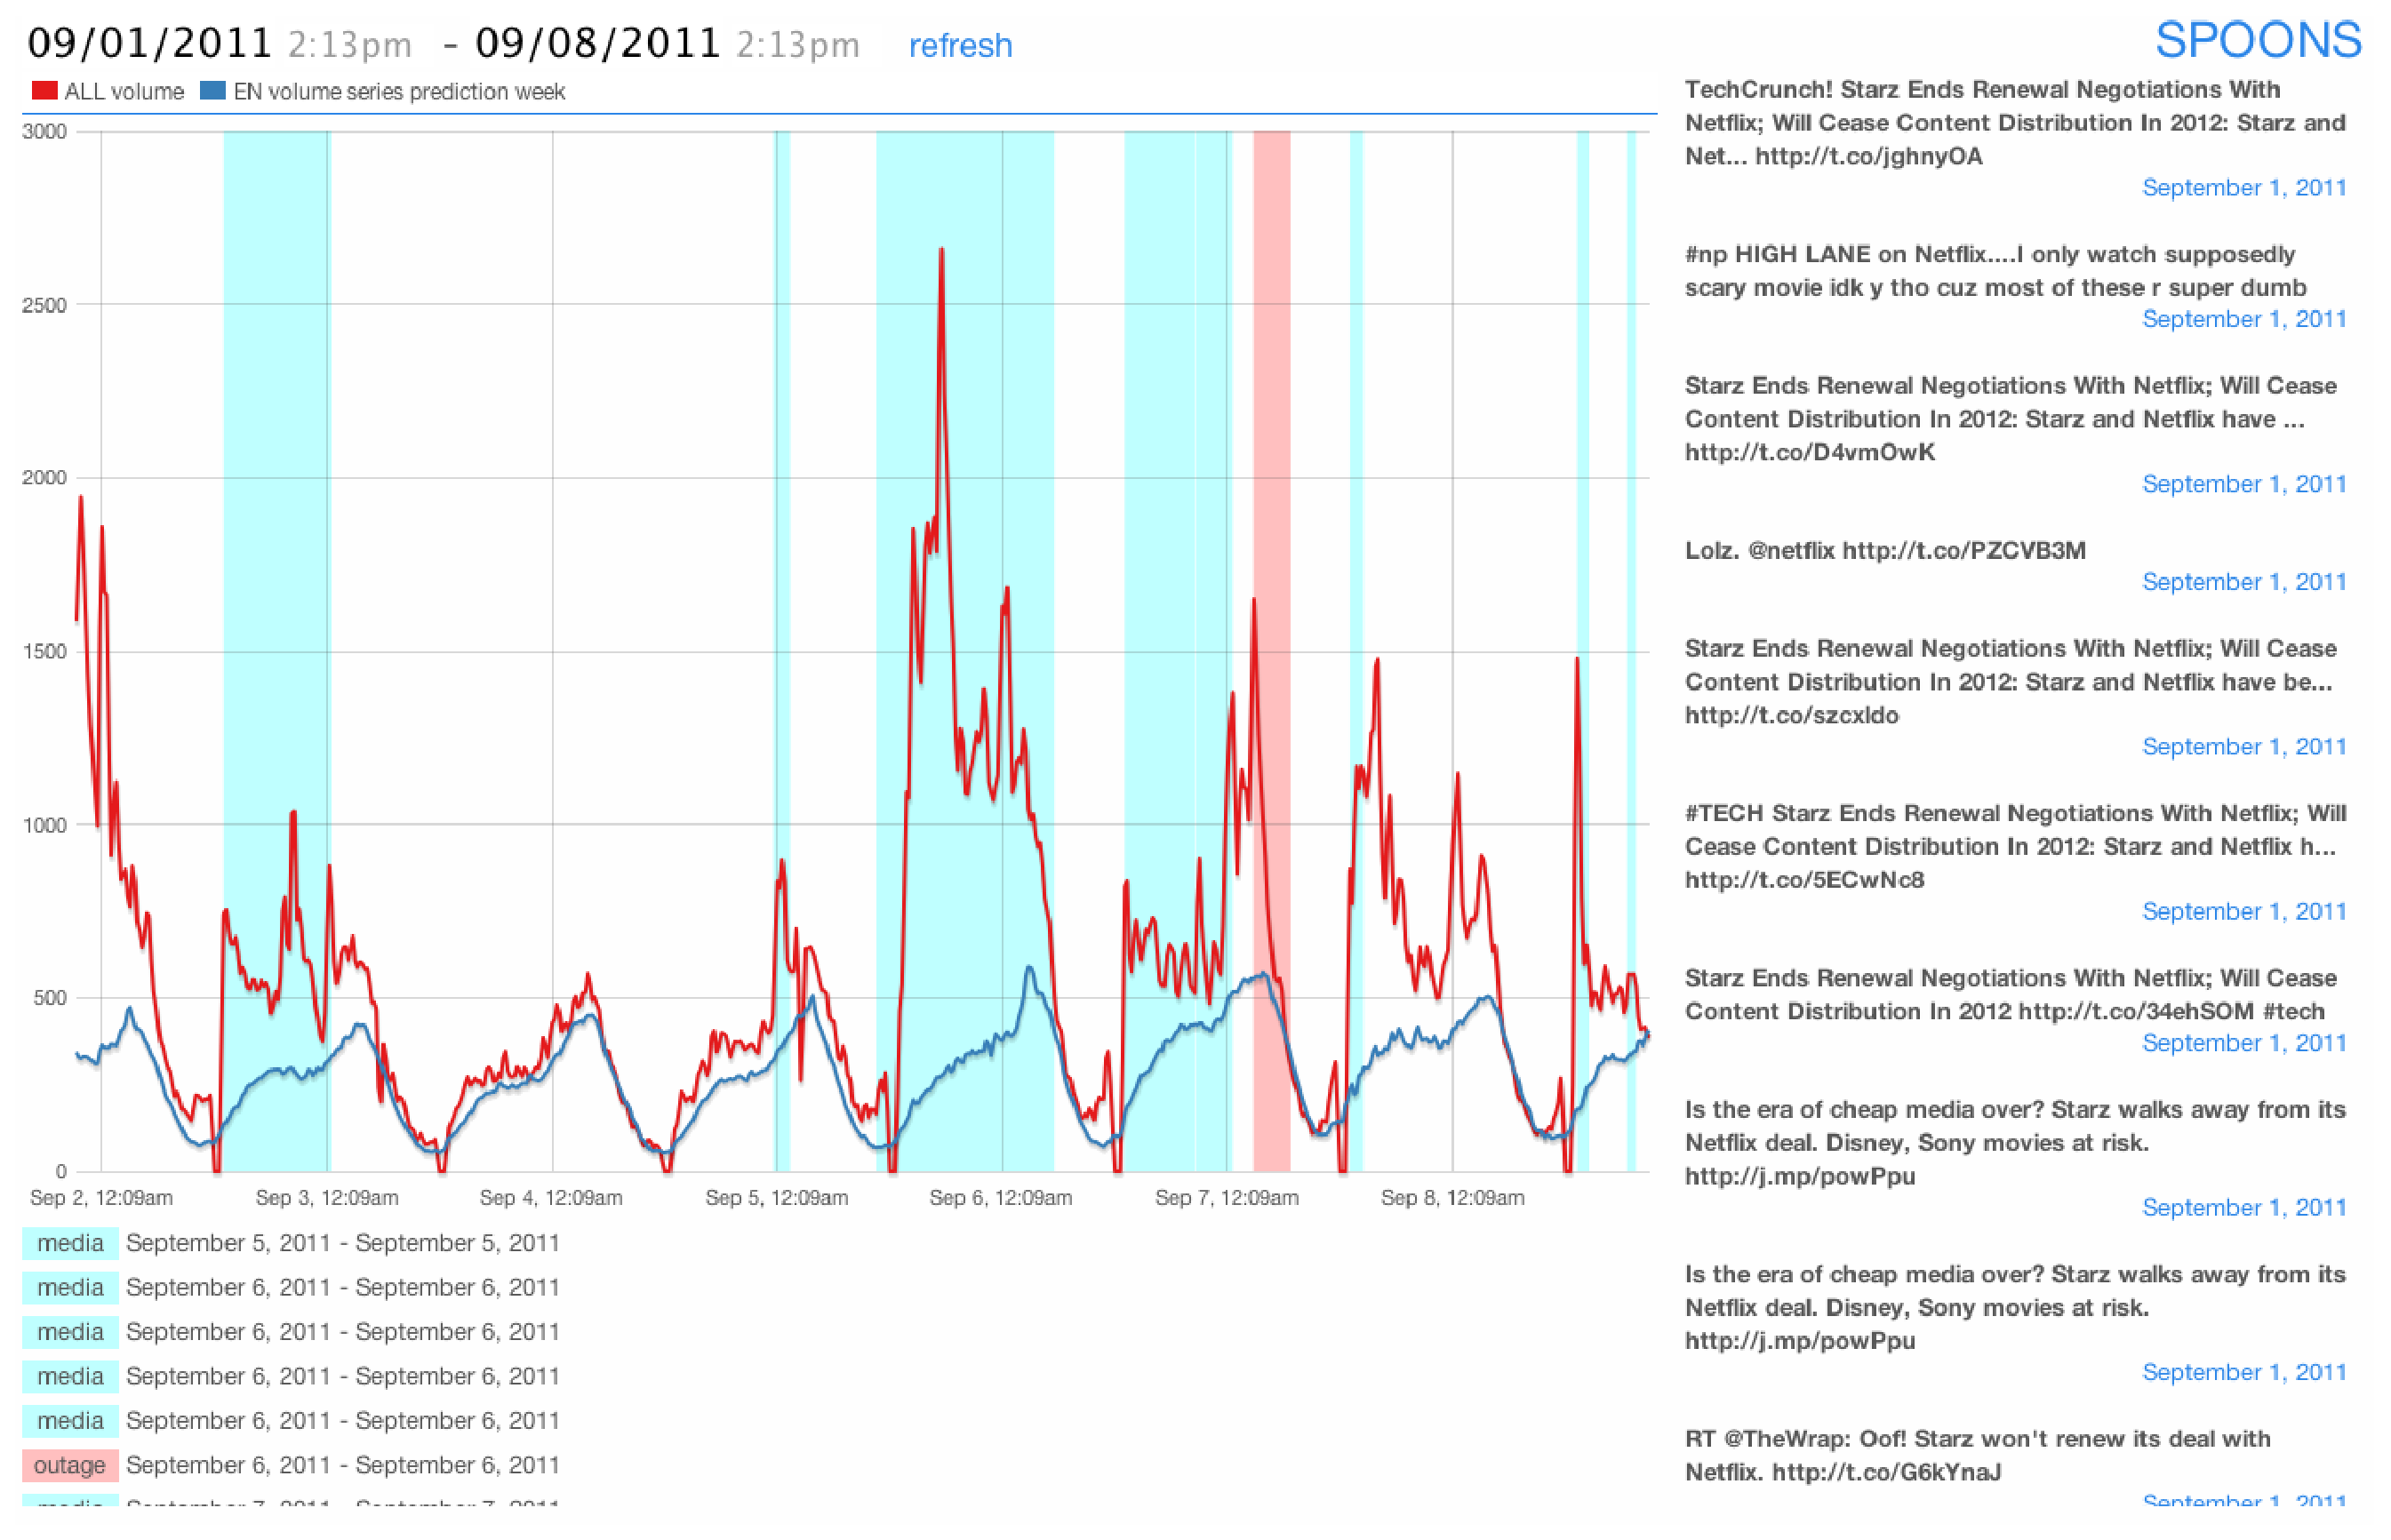
\includegraphics[width=0.8\textwidth]{images/ui.eps}
      \captionfonts
      \caption[SPOONS UI]{The web UI for SPOONS.}
      \label{fig:ui}
   \end{center}
\end{figure}

There are multiple levels of architecture within SPOONS that need to be discussed.
Chapter~\ref{arch-framework} describes the framework architecture (Figure~\ref{fig:frameworkArch}).
The framework architecture describes the relations between the different pieces of the SPOONS framework.
Chapter~\ref{arch-dist} describes both the layout of the different servers involved in the SPOONS system
and the Distribution Model which describes how pieces of work are distributed between the different servers
Finally, Chapter~\ref{arch-database} discusses the architecture of the database that backs SPOONS.

\chapter{Framework Architecture}
\label{arch-framework}
This chapter describes the architecture of the SPOONS framework. The SPOONS framework includes all pieces of SPOONS
that take the data from gathering all the way through to final analysis.

\section{High Level Solution}
\label{arch-framework-highlevel}
The general solution taken by SPOONS consists of four main steps:

\begin{description}
   \item[Collect:]
      Collect tweets from Twitter.
   \item[Process:]
      Convert the tweets from plain text to some form of information that can be analyzed.
   \item[Model:]
      Use the information generated from the previous step to build a mathematical model of the information.
      Use past information to predict what the current model of the data should look like.
   \item[Compare:]
      Compare the two models generated in the previous step. A significant divergence means that there is
      anomalous traffic.
\end{description}

\subsection{Framework Overview}
\label{arch-framework-highlevel-overview}

Figure~\ref{fig:frameworkArch} shows the flow of control and data through the SPOONS framework. Data comes into SPOONS
in the form of Tweets collected by the Gatherers, and leave SPOONS in the form of alerts generated by the Monitors.

\paragraph{Gatherer.}
Gatherers are responsible for collecting documents from a specified data source such as the Twitter Search API.

\paragraph{Database.}
After the tweets are gathered, they are placed in the database. In addition to storing just tweets, the database also stores
configuration data, intermediate calculations, and the results of the Analysis Pipelines.

\paragraph{Control.}
The Control is responsible for controlling the SPOONS server. It maintains data structures with all of the Gatherers and
Analysis Pipelines. It is also responsible for communication with other servers in the SPOONS cluster.

\paragraph{Processor.}
Processors are data transformation utilities that take raw data and puts it in a form that other components can use.

\paragraph{Modeler.}
Modelers are responsible for building a mathematical model of the data and can be split into two groups: \textbf{Predictors} and \textbf{Counters}.
Predictors build a predictive model of the data. Counters build a model of the data that was actually gathered by the system.

\paragraph{Monitor.}
Monitors take the models produced by the Predictors and Counters and compares them. The Monitors are responsible for
making the final decision on about a period of time being anomalous.

\section{Gatherers}
\label{arch-gatherers}
The data enters SPOONS at the Gatherers. The Gatherers run periodically (for Twitter, every two minutes).
Gatherers are asynchronous and not dependent on any other part of the framework. There may be multiple different
Gatherers running on the same machine. Gatherers are abstracted to be able to gather data from any source.
Once the Gatherers obtain their data, they place the data in the database and notify the Control that there is new data
available to the system.

\subsection{Twitter Holes}
\label{arch-twitter-holes}
It is worth noting that sometimes the Twitter Search API fails to return any data. We have not discovered the cause
of this, but Twitter does not report any errors. For unspecified amounts of time the Twitter API reports zero
new tweets. We call these dead zones ``holes''. We have found that a query from a different IP usually does not
experience the same hole. To counteract holes, we run Gatherers on multiple servers and resolve duplicate tweets upon insertion
into the database.

\begin{figure}
   \begin{center}
      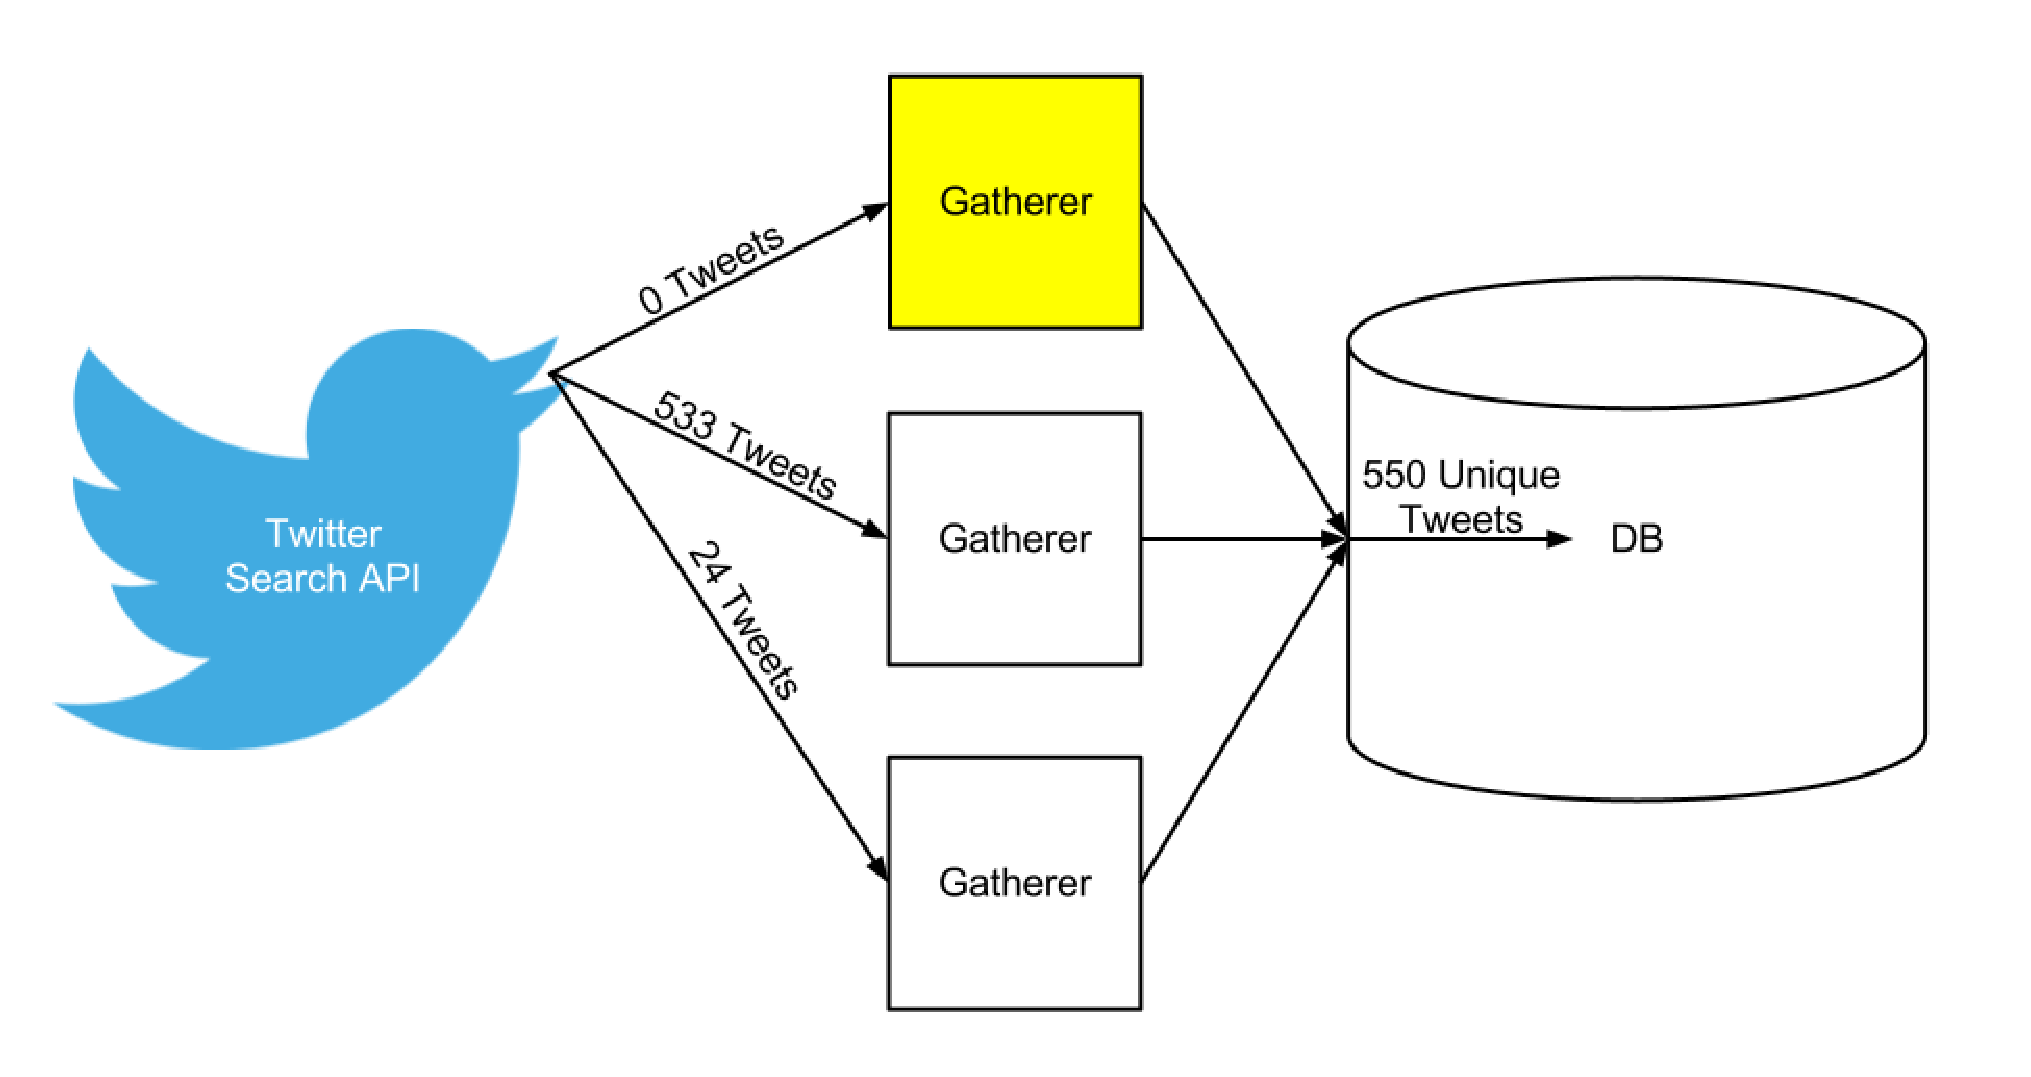
\includegraphics[width=0.9\textwidth]{images/Twitter_Holes.eps}
      \captionfonts
      \caption[Twitter Holes]{One server in a hole is covered by two other gathering servers.}
      \label{fig:twitterHoles}
   \end{center}
\end{figure}

\section{Processors}
\label{arch-processors}
Processors are responsible for processing or transforming data before it goes into the analysis pipelines.
\begin{itemize}
   \item \underline{Classifier Processors}: There exists a Processor for every tweet classifier used in SPOONS (see Chapter~\ref{classifiers}).
   Because of the high number of classifiers used, these constitute the majority of Processors and form the largest unit of work in SPOONS.
   These Processors classify every tweet into one of the nine tweet categories discussed in Section~\ref{class-tweet-classes}.

   \item \underline{Author Processors}: The Author Processors extract the author of tweets and try to establish which authors are credible. These Processors are
   outside the scope of this work and are discussed in other work\cite{cailinThesis}.

   \item \underline{Valence Processors}: The Valence Processors assign a numeric ``happiness'' score to every tweet. How that score is produced is outside the
   scope of this work (see Section~\ref{future-work-kim}).

   \item \underline{Document Frequency Processors}: The Document Frequency Processors maintain term frequencies and inverse document frequencies for the collection
   of tweets in SPOONS.
\end{itemize}

\paragraph{Implementation Notes:}
Unlike most parts of the analysis pipeline, Processors are a shared resource. That is, multiple analysis pipelines
invoke the same Processors. However, it does not make sense to restart the processing once it is started, or to
start another instance of the same Processor for the same data. Processors have a finite amount of data to process and may be cumulative.
To make sure that no redundant work is done, Processors are singleton. When multiple threads call into a Processor to do work, the Processor blocks
all incoming threads until the work is complete. Then, the Processor releases all of the threads that requested the work.
This model allows all the analysis pipelines to share the same Processor without any redundancies.

\section{Analysis Pipelines}
\label{arch-pipelines}
An Analysis Pipeline (also called Analysis Method) is the analytical center of the SPOONS framework.
Pipelines are split into Tasks (see Section~\ref{arch-tasks}) which are chunked units of work.
The exact number and types of Tasks used are different for each pipeline.

The run of an Analysis Pipeline is typically as follows:
\begin{enumerate}
   \item Pre-process incoming traffic.
   \item Model the existing traffic.
   \item Predict what the current traffic should be.
   \item Raise an alert if the existing traffic varies significantly from the predicted traffic.
\end{enumerate}

Every Analysis Pipeline gets its own thread, and there is no interdependence between the different pipelines.
Currently, SPOONS usually runs more than 20 Analysis Pipelines at a time.

\section{Tasks}
\label{arch-tasks}
Tasks are the core unit of computation in SPOONS. Almost everything that can be ``run'' is a Task.
Every Task gets its own thread, and callers into the Task may request that the Task block the calling thread
until the Task is complete.

\paragraph{Implementation Notes:}
Tasks are singleton with respect to the leaf child class.
This ensures that although there there are many different Tasks, every Task can be uniquely referenced.
This singleton behavior is enforced by checking the fully-qualified class name in the Task base class upon construction.
The uniqueness of tasks is very important to SPOONS distribution model discussed in Chapter~\ref{arch-dist}.

\section{Modelers}
\label{arch-modelers}
Modelers are Tasks that are responsible for building a mathematical representation for the data.

\subsection{Predictors}
\label{arch-predictors}
Predictors build a predictive model of the data. For example, we have noticed that tweet volume tends to be
periodic day-to-day and week-to-week. Therefore, a Predictor may model that prediction by guessing that the volume
in the future will be the same as it was the previous week or day.

\subsection{Counters}
\label{arch-counters}
Counters attempt to build a model of data that was actually gathered by the system. Going with the previous example,
the Counter for modeling tweet volume would simply count the number of tweets gathered for a period.

\section{Monitors}
\label{arch-monitors}
Monitors take the models produced by the Predictors and Counters and compares them one point at a time.
If the two models differ significantly, then an alert is raised.
The different types of Monitors are described in detail in Section~\ref{outage-detection-monitors}.
The Monitors are responsible for making the final decision about a period of time being anomalous.

\subsection{Auto-Tuning}
\label{arch-autotuning}
Monitors are the most configurable part of the Analysis Pipeline taking anywhere from two to six configurable parameters.
To find the best set of parameters, the Monitors can automatically run themselves on a training set and search the space of all possible parameters.
They then keep the parameters that result in the best score.
This process is called ``auto-tuning''.

\subsection{Resistance}
\label{arch-resistance}
At any given time, a Monitor is either in a normal, non-alerting, state or an alerting state.
A Monitor's ``resistance'' is its tendency not to move into or out of an alerting state.
The resistance is the number of normal or abnormal observations it needs to be
trigger a state change. Monitors are given resistance because otherwise an outliers could cause
a Monitor to rapidly switch between alerting and normal states.
There currently are three different methods of observing resistance.
The method of resistance as well as the resistance thresholds can also be auto-tuned.

\subsubsection{Fighting Resistance}
\begin{table}[H]
   \begin{center}
      \begin{tabular}{|c|p{9cm}|c|}
         \hline
            Parameter & Description & Restrictions \\
         \hline
            A & The number the counter must reach to enter an alerting state. & $ A > 0 $ \\
         \hline
            R & The number the counter must reach to enter a normal state. & $ R > 0 $ \\
         \hline
      \end{tabular}
   \end{center}
\end{table}

Fighting resistance counts every time that there is a normal period as a +1, and every time there is
an anomalous period as a -1. If the counter reaches $-A$, then the Monitor is put into an alerting state.
If the counter reaches $R$, then the Monitor is put into a normal state.

\subsubsection{Continuous Resistance}
\begin{table}[H]
   \begin{center}
      \begin{tabular}{|c|p{9cm}|c|}
         \hline
            Parameter & Description & Restrictions \\
         \hline
            A & The number the counter must reach to enter an alerting state. & $ A > 0 $ \\
         \hline
            R & The number the counter must reach to enter a normal state. & $ R > 0 $ \\
         \hline
      \end{tabular}
   \end{center}
\end{table}

Continuous resistance must get $A$ continuous anomalous observations to enter an alerting state, and $R$ continuous normal
observations to enter a normal state.

\subsubsection{Window Resistance}
\begin{table}[H]
   \begin{center}
      \begin{tabular}{|c|p{9cm}|c|}
         \hline
            Parameter & Description & Restrictions \\
         \hline
            W & The window size. & $ W > 0 $ \\
         \hline
            C & The number of anomalous observations necessary for an alerting state. & $ 0 < C <= W $ \\
         \hline
      \end{tabular}
   \end{center}
\end{table}

Window resistance remembers $W$  previous observations as being normal or anomalous. If the number of anomalous
observations is or exceeds $C$, then an alerting state is declared. Otherwise, the Monitor stays in a normal state.

\subsection{Smoothers}
\label{arch-smoothers}
The Monitors have a chance to smooth the data before it gets analyzed.
Smoothers take in a stream of data.
As with resistance methods, different smoothers and smoothing parameters can be auto-tuned.

\subsubsection{No Smoother}
Do not smooth. If this smoother is put into the parameter search space, then the effects of no smoothing can be seen.

\subsubsection{Moving Mean Smoother}
\begin{table}[H]
   \begin{center}
      \begin{tabular}{|c|c|c|}
         \hline
            Parameter & Description & Restrictions \\
         \hline
            W & The window size. & $ W > 0 $ \\
         \hline
      \end{tabular}
   \end{center}
\end{table}

The Moving Mean Smoother works by taking the mean in a sliding window of size $W$.
This Smoother tolerates a smaller window if there is not enough data available.
Therefore, this Smoother always outputs a number for every number in the input stream.

\section{Control}
\label{arch-control}
The Control is the center of a SPOONS instance. It handles the flow of all control and has the ability to start and
stop any Task or Analysis Pipeline on demand. It holds references to all the threads for the Gatherers and Analysis Pipelines.
The Control handles all the setup and tear down in the system.

There are different types of Controls that decide the behavior of SPOONS on each respective server.
There are three types of Controls: \textbf{Master Control}, \textbf{Worker Control}, and \textbf{Single Control}.
The Control is singleton with respects to the base class.
Therefore, only one instance of any type of Control can be active on a server at any given time.

\paragraph{Implementation Notes:}
The Control is very careful to never allow anyone to own a reference to the currently running Control.
All requests to the Control are made statically to the ``Control'' base class.
The base class then forwards the request onto the specific instance of Control currently active on the server.
This is done so that the rest of the SPOONS system never knows what kind of Control is currently active.
Because of that, a server can be switched between different roles without restarting the system or notifying any other components of the SPOONS system.

\subsection{Master Control}
\label{arch-master-control}
The Master Control is the Control that is responsible for the controlling SPOONS when it is in distributed mode.
The Master Control maintains information on all the active worker servers including what Tasks are currently assigned to them.

\paragraph{Implementation Notes:}
The Master Control maintains ``shallow execution'' of every pipeline in the system.
This means that this control runs each pipeline, but then distributes work for each pipeline as the work is generated.

\subsection{Worker Control}
\label{arch-worker-control}
Worker Controls do not take any initiative to run any tasks. Instead, they just wait for a Master Control to tell them what to do.

\subsection{Single Control}
\label{arch-single-control}
The Single Control is for a SPOONS instance that wants to run on a single server.

\chapter{Distributed Computation Model}
\label{arch-dist}

\begin{figure}
   \begin{center}
      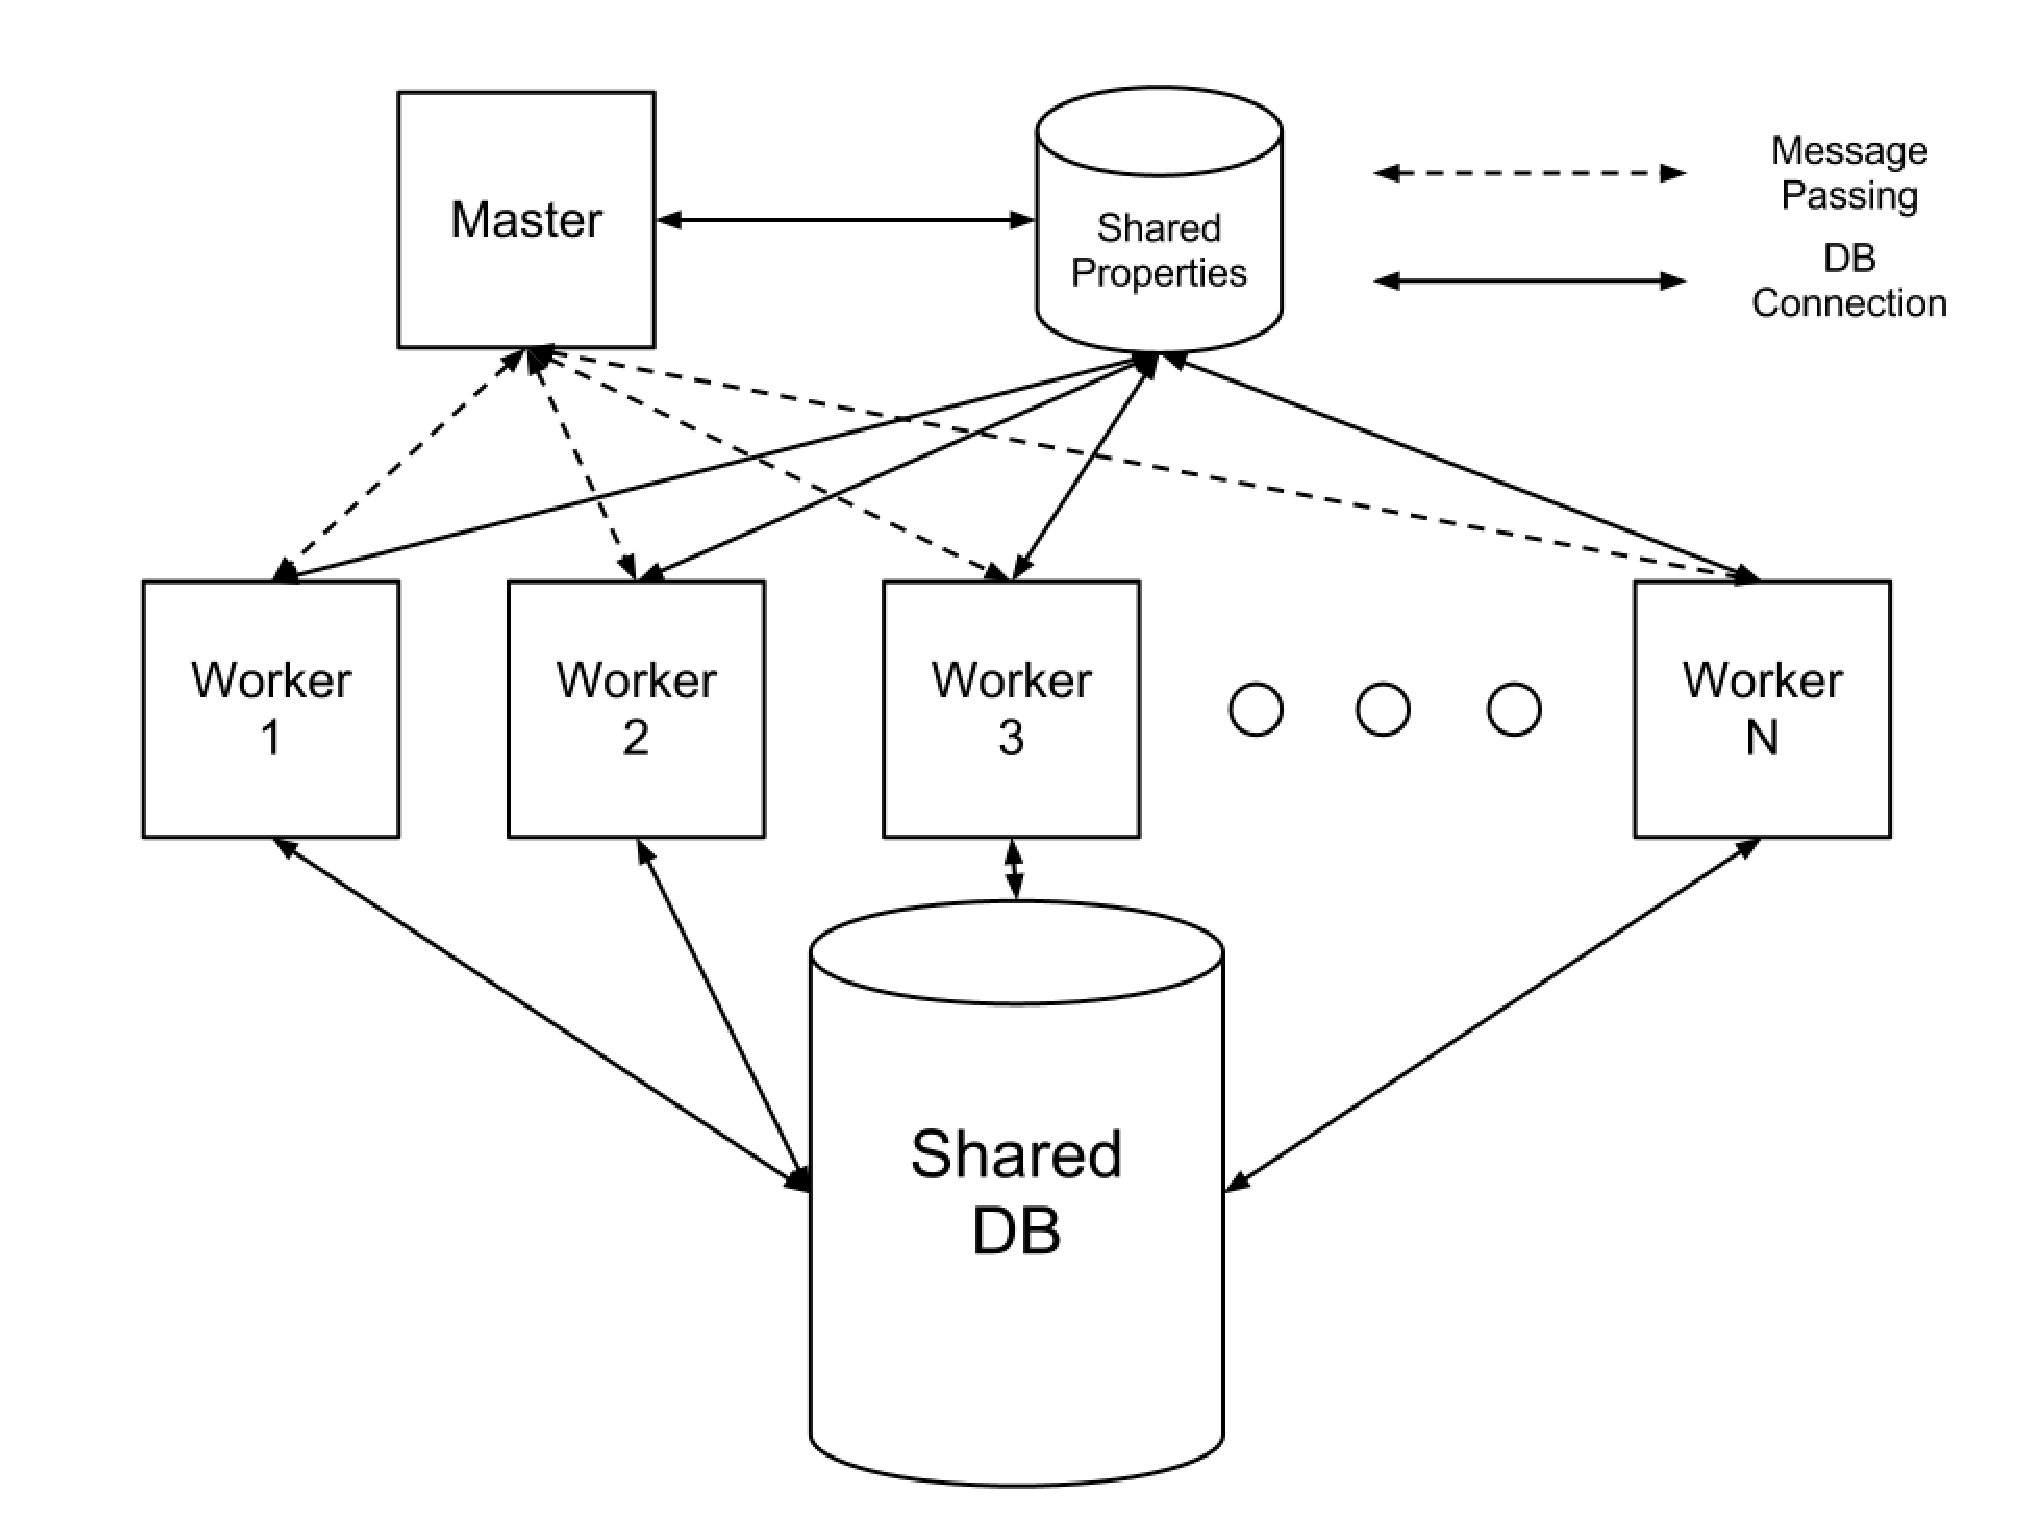
\includegraphics[width=0.8\textwidth]{images/SPOONS_Server_Architecture.eps}
      \captionfonts
      \caption[SPOONS Server Architecture]{The server architecture of the SPOONS system.}
      \label{fig:serverArch}
   \end{center}
\end{figure}

\begin{figure}
   \begin{center}
      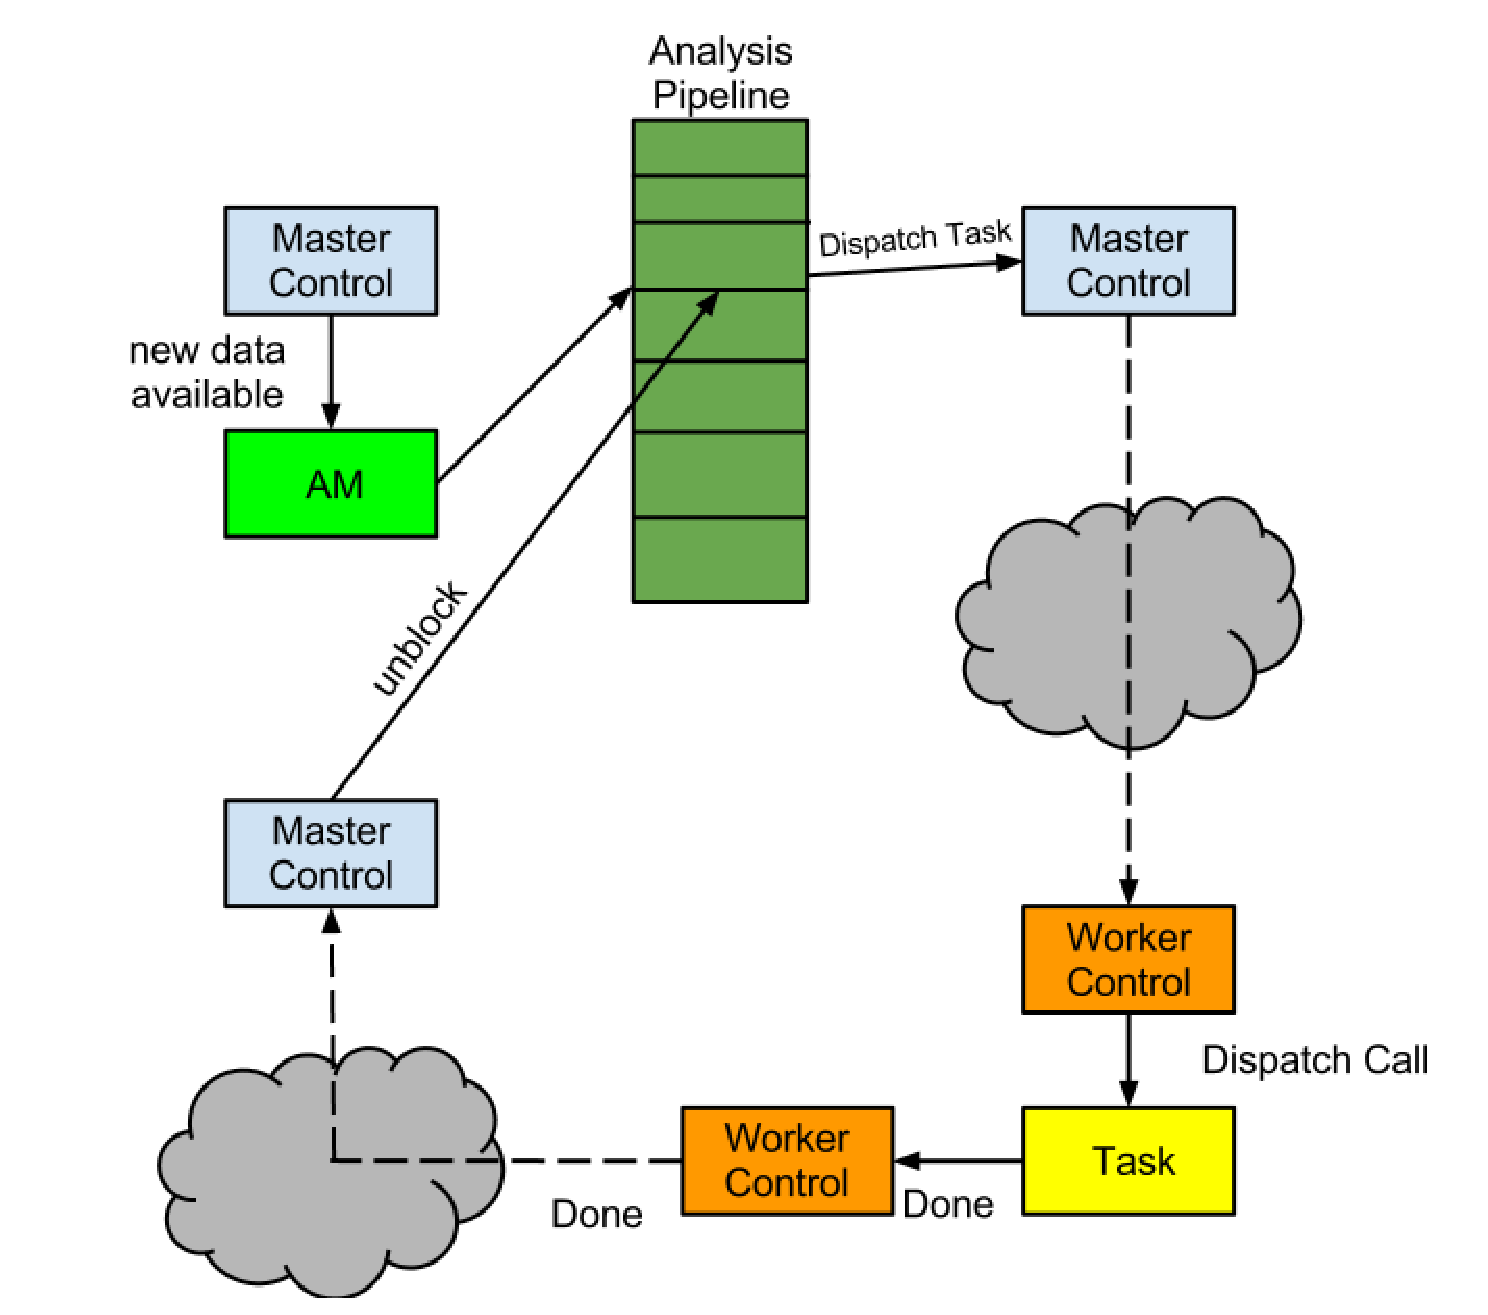
\includegraphics[width=0.8\textwidth]{images/SPOONS_Distributable_Task_Control_Flow.eps}
      \captionfonts
      \caption[SPOONS Distributable Task Flow]{The control flow for distributable tasks.}
      \label{fig:taskFlow}
   \end{center}
\end{figure}

As discussed before, SPOONS is a multi-server system (Fig~\ref{fig:serverArch}).
The SPOONS system uses the master/worker paradigm with a single master and $N$ workers.

All of the servers share two resources: the primary database and a NoSQL property store.
When a master or worker comes online, it inserts an entry for itself into the shared property store.
If the new server is a worker, it alerts the current master about its existence, and visa-versa,
if the new server is a master. In addition, all workers are required to heartbeat to the master every
15 seconds and the master heartbeats to the workers every 15 seconds. Using this system, the master
always knowns about all of the workers and the worker always knows about the current master.
When a server misses three heartbeats, the server expecting that heartbeat assumes that the server has
gone down.

\section{Distribution Requirements}
\label{arch-dist-requirements}
The design of the SPOONS distribution model was dominated by two main concerns: performance and usability.

\paragraph{Performance.}
SPOONS is a real-time system. Any attempt at distribution cannot compromise the response time of the system.
In addition, SPOONS has to be able to survive a server dying. These two concerns led to three requirements:

\begin{itemize}
   \item Efficiency: A distributed SPOONS should have comparable response time to a single server SPOONS.
   \item Fault Tolerance: SPOONS should be able to survive any non-database server failing.
   \item Scalability: Scaling a SPOONS cluster should be straightforward.
\end{itemize}

\paragraph{Usability.}
SPOONS is meant to be a general real-time analysis system that many different types of people can use.
The average developer using SPOONS should be concerned only with the framework level.
Server, network, and distribution semantics should remain transparent to a user of the framework.
To make a distributed SPOONS easy to use for a developer working with the framework, three requirements
are stipulated:

\begin{itemize}
   \item DB: There should be one database, and a framework developer should not have to do anything that is not required on a simple single-server system.
   \item Framework Complexity: All distribution specifics should be hidden from the framework developer.
   \item Single Mode: SPOONS should be able to run on a single server.
\end{itemize}

\section{Distribution Assumptions}
\label{arch-dist-assumptions}
The SPOONS distribution model relies on two assumptions about the system: every server contains
exactly the same data in memory and every Task can be uniquely referenced.

\subsection{Same Data}
SPOONS assumes that every server has the same data in memory on every server.
This means that not only does every server need to have the same data structures in memory,
but also that every server needs to have the same classes instantiated. The only exception to this
assumption is the Control. Depending on the role of the server, a different Control is
instantiated. Because of this assumption, we do not have to worry about active replication
between servers or a worker being asked to do work that requires a class that is not instantiated.

\subsection{Uniquely Referenced Tasks}
As stated in Section~\ref{arch-tasks}, Tasks are the basic unit of work inside SPOONS.
When a worker is told to execute some work, it is being asked to execute a specific Task with specified
parameters. Therefore, Tasks need to be able to be referenced by a key that can be serialized and
sent over the wire from the master to the worker.

\section{Distributable Tasks}
\label{arch-dist-tasks}
Distributable Task is a subclass of Task that provides the distribution mechanism for Tasks.
When a Task is to be distributed, the Distributable Task calls into the Control and requests that
the Control distributes it. The next step varies depending on the type of Control that is active:

\subsection{Master Control}
The Task distributing control flow is described in Figure~\ref{fig:taskFlow}.
A Master Control blocks the calling thread and send a message to a selected worker\footnote{The
current scheduling algorithm chooses the worker that has the fewest Tasks currently assigned to it.} telling it to
run the Task with given parameters. The message that goes to the worker just contains the Task's unique identifier
and the parameters to the Task's run. When the Task is complete, the Worker Control sends the Task's return
status back to the Master Control. When the master receives a message from the worker that the requested Task
has completed its run, it resumes the original calling thread and have it return with the return status given
by the worker.

\subsection{Worker Control}
Worker Controls do not distribute Tasks.
Because Tasks are atomic units of work, Tasks are not supposed to call other Tasks.
If Task A calls upon a Worker Control to distribute a Task B, then that means that Task A has violated
its own atomicity. This is considered a violation of the framework and causes the Worker Control to throw an error.

\subsection{Single Control}
Instead of blocking the calling thread like in the Master Control, a Single Control
just uses the calling thread to run the Task. When the Task is complete,
the Single Control returns control to the caller.

\section{Shared Properties}
\label{arch-props}
As previously stated, all servers must maintain a consistent in-memory view of the system.
This can be troublesome if a Task needs to maintain cumulative settings or member datum.
Not only will this data need to be consistent on all the servers, but it also needs to maintain this
data between starts and stop of the system.
An Analysis Pipeline should be able to be interrupted at any moment, and then restarted later without losing data or its place.

To enforce these restrictions, SPOONS uses a shared property store. The shared property store is a MongoDB server.
Whenever a Task needs to store member datum, it places the data in the shared store, making the data available to any server in the cluster.
A Task can first be run to completion on Server A and then, when new data is available, run on Server B.
Because the Task stores the necessary information in the shared property store,
Server B can have all the information gained from the run on Server A and not lose any positional information.

In addition to storing shared properties, the shared property store houses information on every active server.
When a server comes online, it queries the property store to find all the other active servers and inserts itself into
the store. If a server fails to heartbeat, then the rest of the cluster that is still active removes the entry for that server from the property store.

\chapter{Database}
\label{arch-database}
SPOONS is backed by a MySQL database. SPOONS currently uses 225 tables and 35 stored procedures. The 225 tables are further divided into
six different categories that are used in different stages of the analysis pipeline. In addition to tweets,
configuration data, intermediate calculations, analysis results, and final alerting decisions are stored in the database. Keeping all of this
data allows the users to look back at any point in time for reference or debugging.

The database uses naming and schema conventions to maintain organization on its tables. The naming and schema conventions allow different
components of the Analysis Pipeline to be interchanged without any need to change/reprocess the data. In addition the conventions allows the UI
to represent new tables without the need for specifying them.

\section{Tables and Schemas}
\label{arch-database-tables}
Each stage in an analysis pipeline generally stores some information in the database. Because each stage generally deals with similar
types of data, these tables are considered to be in the same group. We enforce group membership using hints in the table names. For example, the
table name ``\texttt{RESULT\_EN\_class\_heuristic\_bayes\_net}'' gives five hints as to the type of the table.

\begin{enumerate}
   \item \texttt{RESULT} - Marks this table as a result table. This means that it is guaranteed to be shown in the UI.
   \item \texttt{EN} - The language of the tweets that were input into this method.
   \item \texttt{class} - Indicates that this these results are output from a tweet classifier.
   \item \texttt{heuristic} - States that the type of classifier used was a heuristic classifier.
   \item \texttt{bayes\_net} - The name of the classifier used.
\end{enumerate}

Using all of these hints, the UI can then ask for data for specific types of tables (eg. all result tables that are for English tweets).

The six different top level categories that SPOONS recognizes are:

\begin{enumerate}
   \item CALC - These tables store intermediate results in analysis pipelines. CALC tables are typically only used when large sets of past data are needed for cumulative models. They are never shown to the UI.
   \item CONFIG - Contains information that analysis methods used to configure themselves before runs. These tables have been mostly replaced with the shared property store (see Section~\ref{arch-props}).
   \item DATA - Raw input data. These tables are generally the output from the Gatherers.
   \item META - Contains information that is not analyzed, but required by the system. For example, the different classes that the classifiers use along with descriptions of each class.
   \item RESULT - These tables are output from some analysis pipeline. They are guaranteed to be shown in the UI. These tables typically contain time series of some analytical signal.
   \item TEST - These tables are used for debugging and development. They are never shown in a user-facing UI, however may be shown in development UIs.
\end{enumerate}

The full schemas for select tables are described in Appendix~\ref{appendix-db-schema}.

\subsection{Data Flow}
\label{arch-database-data-flow}
The flow of data through the different types of tables is described in Figure~\ref{fig:db-data-flow}.
The data originates from the Gatherers and is moved into DATA tables. Information from
DATA, CONFIG, and META tables are analyzed and placed in either CALC, RESULT, or TEST tables.
At a later time the data from CALC tables is further analyzed and the results are placed in a RESULT table.

\begin{figure}
   \begin{center}
      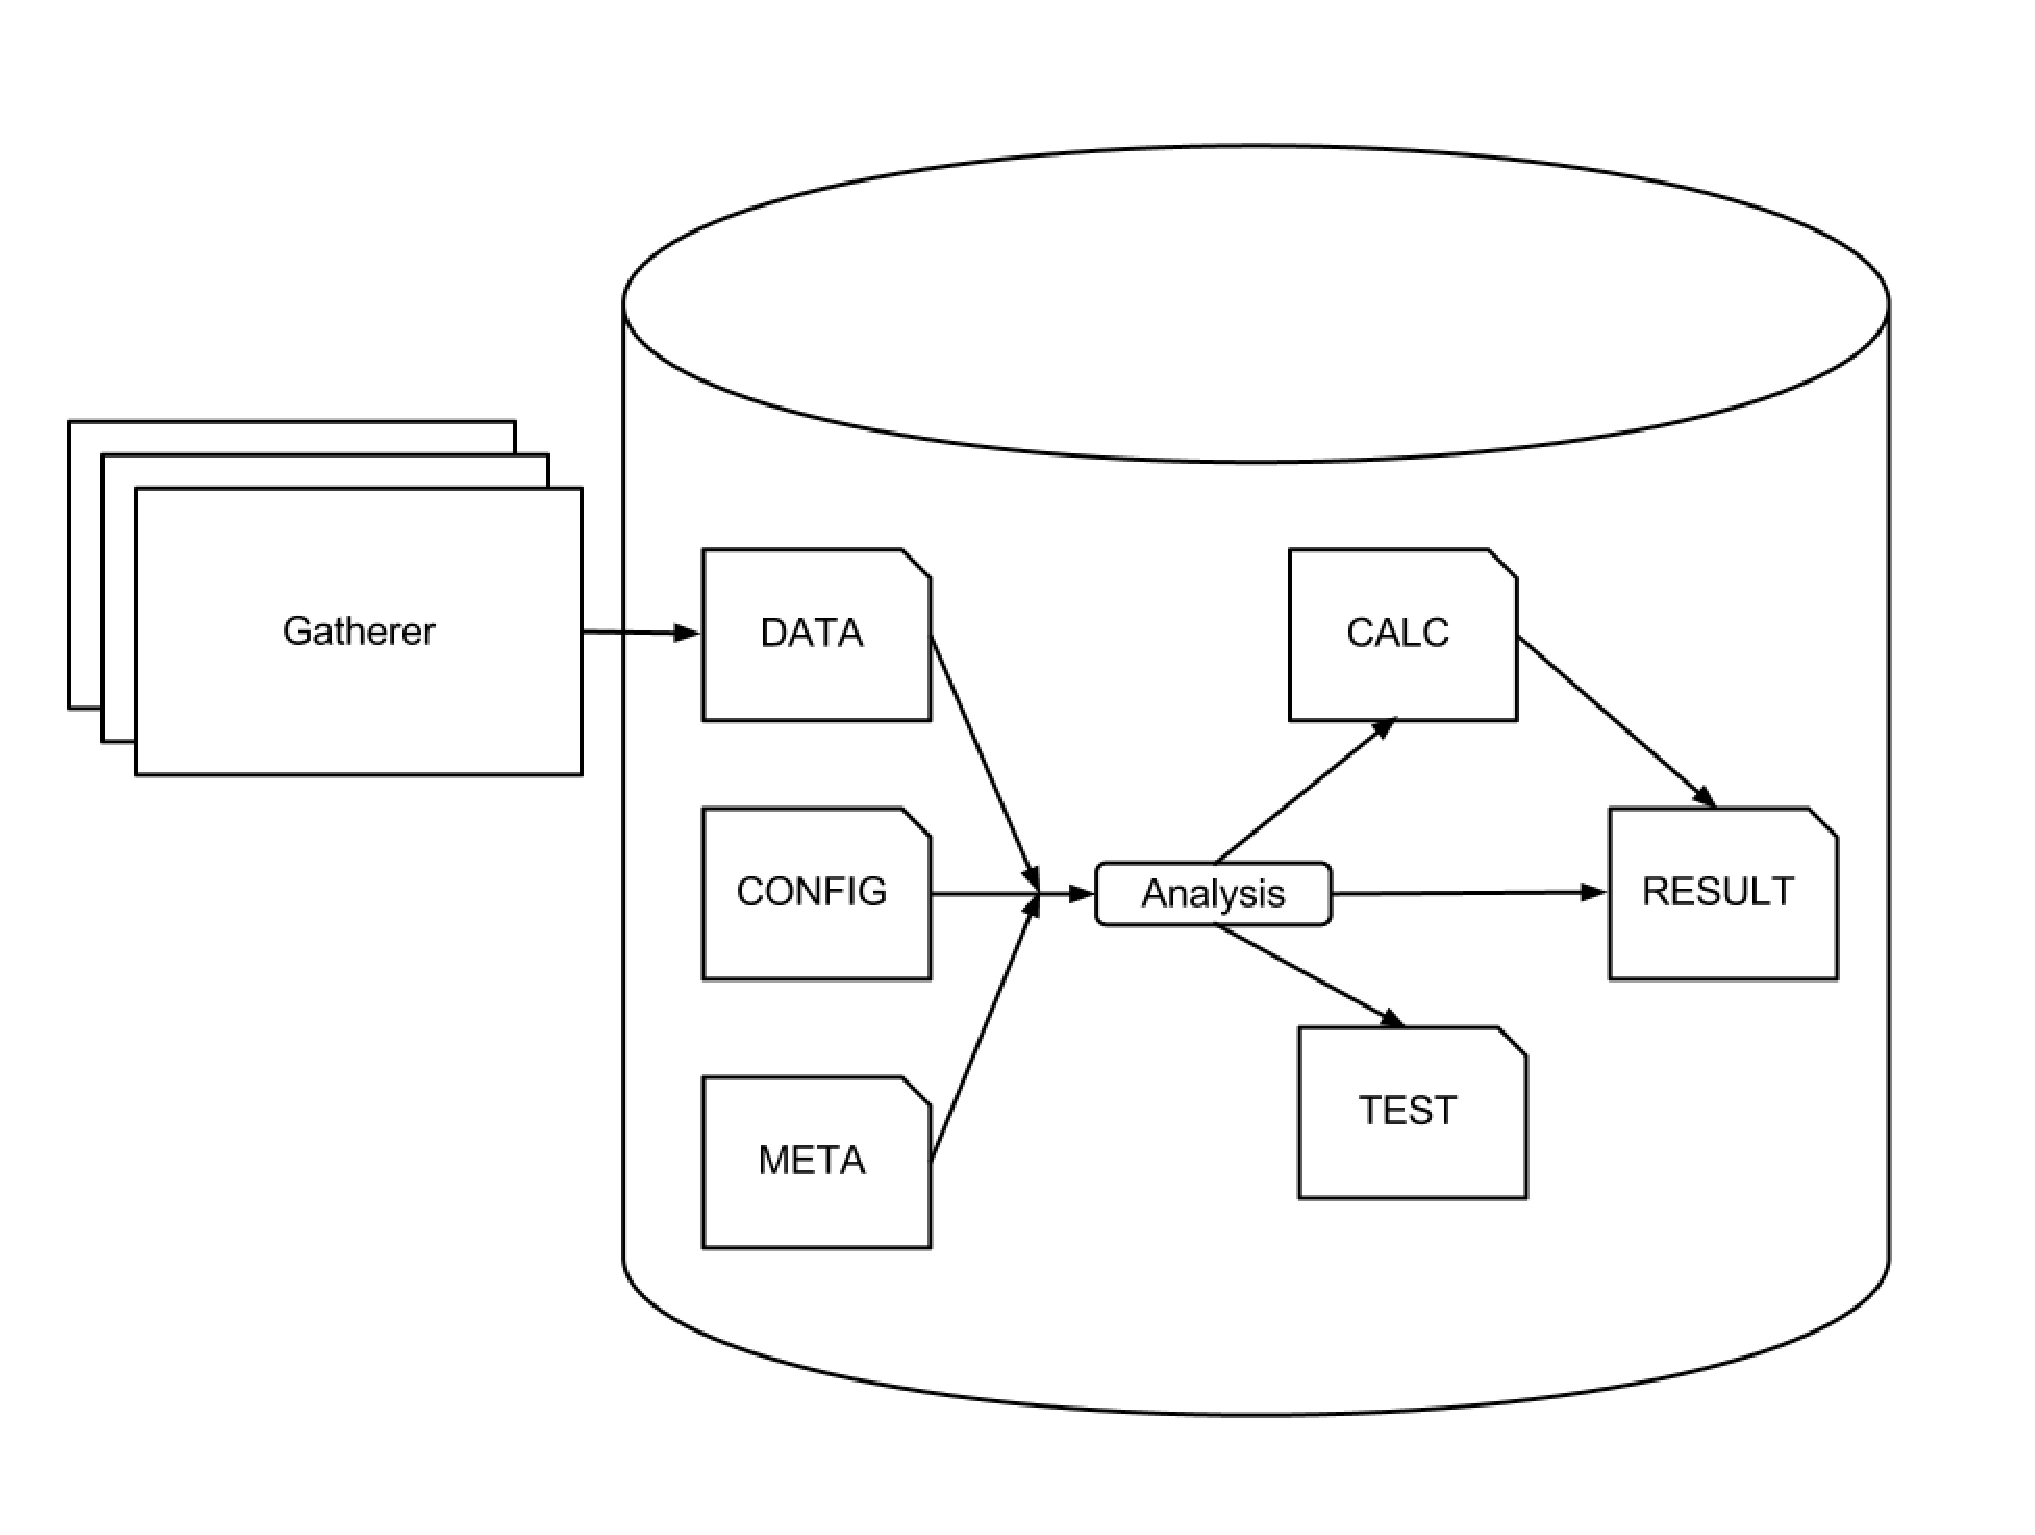
\includegraphics[width=0.8\textwidth]{images/DB_Data_Flow.eps}
      \captionfonts
      \caption[Database Data Flow]{The flow of data through the different types of tables in SPOONS.}
      \label{fig:db-data-flow}
   \end{center}
\end{figure}

\subsection{Tweets Table}
\label{arch-database-tables-tweets}
As the most used and important table in the database, the table that houses all of our tweets, ``DATA\_tweets'', gets special attention.

The tweets table contains ten attributes which are described in Table~\ref{table:tweet-attributes}.

\begin{table}
   \begin{center}
      {\Large Data\_tweets Schema}
      \begin{tabular}{|l|p{12cm}|}
         \hline
            Name & Description
         \tabularnewline\hline
            \textsf{id} & An auto-incremented primary key.
         \tabularnewline\hline
            \textsf{twitter\_id} & The unique id Twitter gives to a tweet.
         \tabularnewline\hline
            \textsf{published} & The epoch time that the tweet was posted according to Twitter.
         \tabularnewline\hline
            \textsf{content} & The raw content of the tweet.
         \tabularnewline\hline
            \textsf{source} & Information on where the tweet was posted from (eg. from a third party app).
         \tabularnewline\hline
            \textsf{lang} & The suggested language of the tweet.
         \tabularnewline\hline
            \textsf{author} & The author of the tweet.
         \tabularnewline\hline
            \textsf{frame\_id} & The frame that this tweet falls into, has an index on it.
         \tabularnewline\hline
            \textsf{place} & Information on where the tweet was posted from. This is a JSON structure and may contain fields such as ``city'' and ``state''.
         \tabularnewline\hline
            \textsf{geo} & Geographical coordinates of place.
         \tabularnewline\hline
      \end{tabular}
   \end{center}
   \caption[Database Tweet Attributes]{The database attributes used to describe tweets.}
   \label{table:tweet-attributes}
\end{table}

\subsubsection{Frames}
Inside SPOONS, we use a ``frame'' as the atomic unit of time. Currently, a frame corresponds to a minute. Bucketing the tweets into frames allows us to
gain a natural aggregation and smoothing. It also provides a natural index. Maintaining an index on \textit{frame\_id} allows quick retrieval of
time series data which is the primary task of SPOONS. Because insertions are generally chronological, insertions are also quick and do not require a
rebuild of the B-Tree index\cite{innodb}.

\section{UI Stored Procedures}
\label{arch-database-sp}
In addition to utility procedures, the database holds many stored procedures used by the UI.
This keeps the UI fairly stable in the face of database changes.

\subsection{Expected Schemas}
\label{arch-database-sp-schemas}
The UI Stored Procedures look for 6 distinct name/schema combinations all of which are required to have the ``\texttt{RESULT}'' prefix.
The different schema requirements are shown in Table~\ref{table:ui-expected-schema}, and described below:

\begin{table}
   \begin{center}
      \begin{tabular}{|l|p{12cm}|}
         \hline
            Schema Name & Required Columns
         \tabularnewline\hline
            Volume & \textsf{start\_frame}, \textsf{value}
         \tabularnewline\hline
            Volume Prediction & \textsf{start\_frame}, \textsf{prediction}
         \tabularnewline\hline
            Valence & \textsf{start\_frame}, \textsf{value}
         \tabularnewline\hline
            Valence & \textsf{start\_frame}, \textsf{prediction}
         \tabularnewline\hline
            Class & \textsf{start\_frame}, \textsf{undecided}, \textsf{media}, \textsf{neutral}, \textsf{snafu}, \textsf{watching}, \textsf{response}, \textsf{complaint}, \textsf{refuse\_to\_rate}, \textsf{happy}
         \tabularnewline\hline
            Group & \textsf{start\_frame}, \textsf{media}, \textsf{bad}, \textsf{other}
         \tabularnewline\hline
      \end{tabular}
   \end{center}
   \caption[Stored Procedure UI Expected Schema]{The different types of schemas that the UI looks for in RESULT tables.}
   \label{table:ui-expected-schema}
\end{table}

\begin{description}
   \item[Volume.]
   This schema is for tables that contain time series information about tweet volumes.
   This includes tables that hold the time series for the total Netflix-related Twitter traffic.

   \item[Volume Prediction.]
   These tables contain time series that are predictive models of Netflix-related Twitter traffic.

   \item[Valence.]
   These tables contain time series for estimates of the current sentiment about Netflix.

   \item[Valence Prediction.]
   These tables contain time series that are predictive models of the sentiment about Netflix.

   \item[Class.]
   These tables contain time series for the volume of tweets that were classified into
   each of the nine categories described in Section~\ref{class-tweet-classes}.

   \item[Group.]
   These tables contain time series for the volume of tweets that were classified into
   each of the thee different groupings described in Section~\ref{class-tweet-groups}.
\end{description}

The stored procedures further divides the tables by language. The currently recognized languages are English,
Spanish, and Portuguese.

% TODO(eriq): Better name
\part{Analysis}
\label{analysis}

\chapter{Classifiers}
\label{classifiers}

\section{Why Classification?}
\label{class-why}
Classification helps discover Netflix service outages by differentiating between different types of Twitter traffic.

Figure~\ref{fig:normal-traffic} shows the normal pattern of Netflix-related Twitter traffic over the course of a single week.
The peaks appear at around 7pm PST and the valleys are around 2am PST.
This kind of pattern is very regular and repeats weekly during normal times.
However, where there is some sort of event, the traffic develops spikes. Figure~\ref{fig:anomalous-traffic} shows a period with two
anomalous spikes. However, sampling tweets from the different spikes hints that the causes for the two spikes
are very different. Figure~\ref{fig:linkless-traffic} shows tweets sampled from each spike. The left spike is composed mostly
of tweets indicating that Netflix is experiencing a service outage. The right spike however, is composed mainly of tweets linking to
a news article about Netflix. Therefore, we see that not only service outages generate spikes in Netflix-related Twitter traffic.

This is where classifiers become useful. If tweets can be placed into different classes according to their type,
then the different types of traffic can be differentiated. Figure~\ref{fig:classified-traffic} shows the result of classifying
the tweets and then building time series of the classes respective traffic. It becomes obvious that the spike on the left is caused by
outage related traffic and that the spike on the right is caused by media related traffic.

\begin{figure}
   \begin{center}
      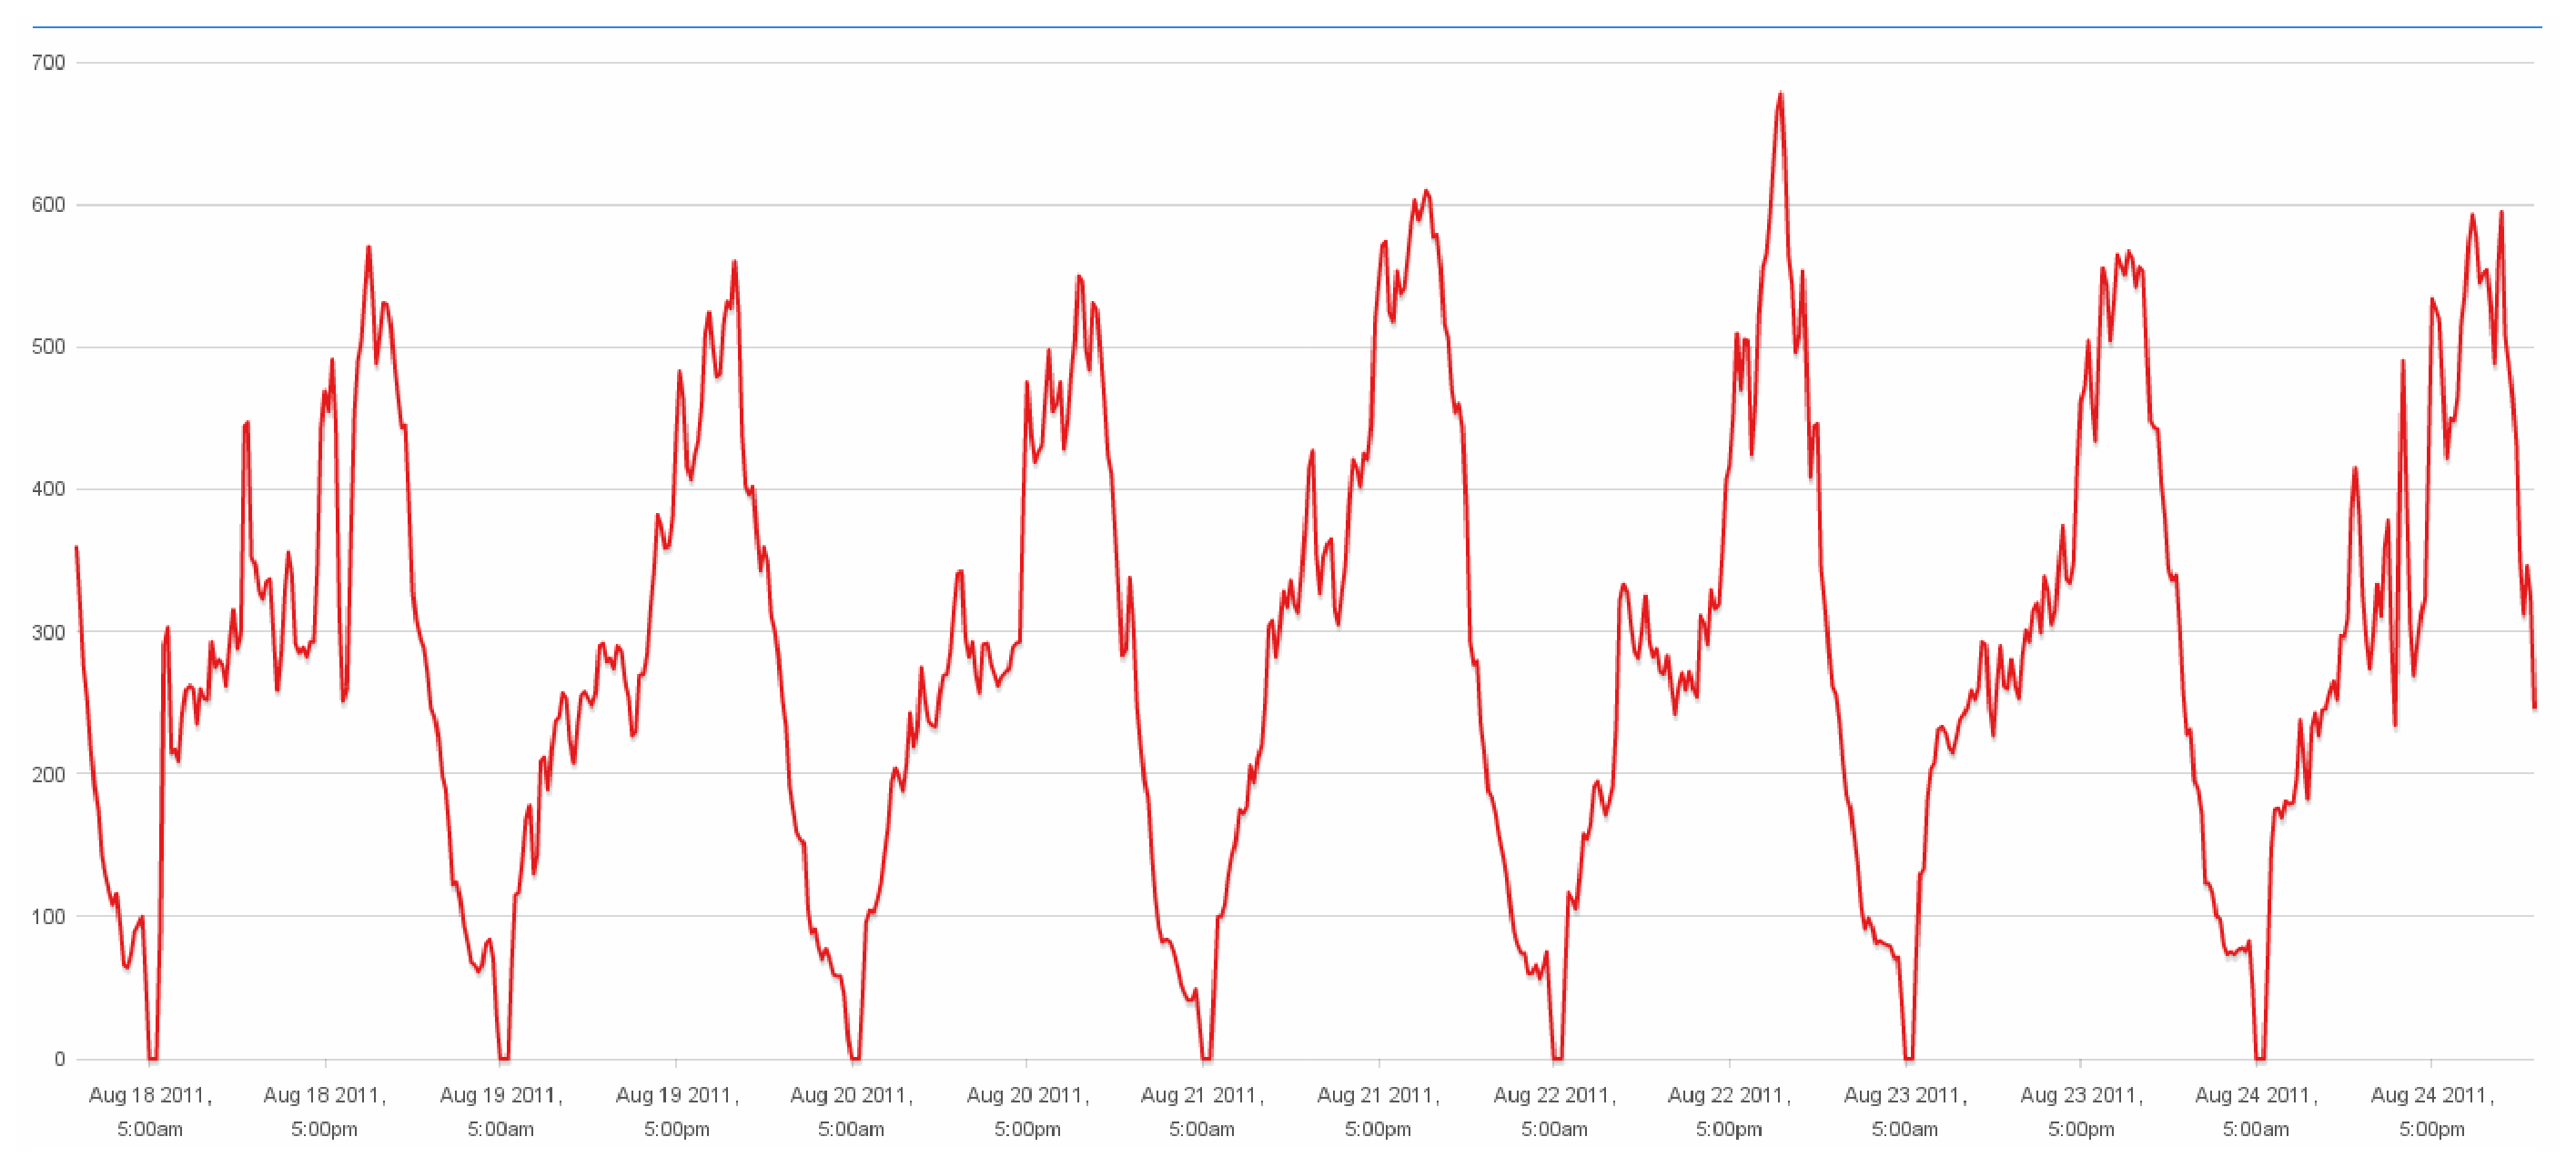
\includegraphics[width=0.8\textwidth]{images/Normal_Traffic.eps}
      \captionfonts
      \caption[Normal Traffic]{A week's worth of Netflix-related Twitter traffic. Notice the daily periodicity.}
      \label{fig:normal-traffic}
   \end{center}
\end{figure}

\begin{figure}
   \begin{center}
      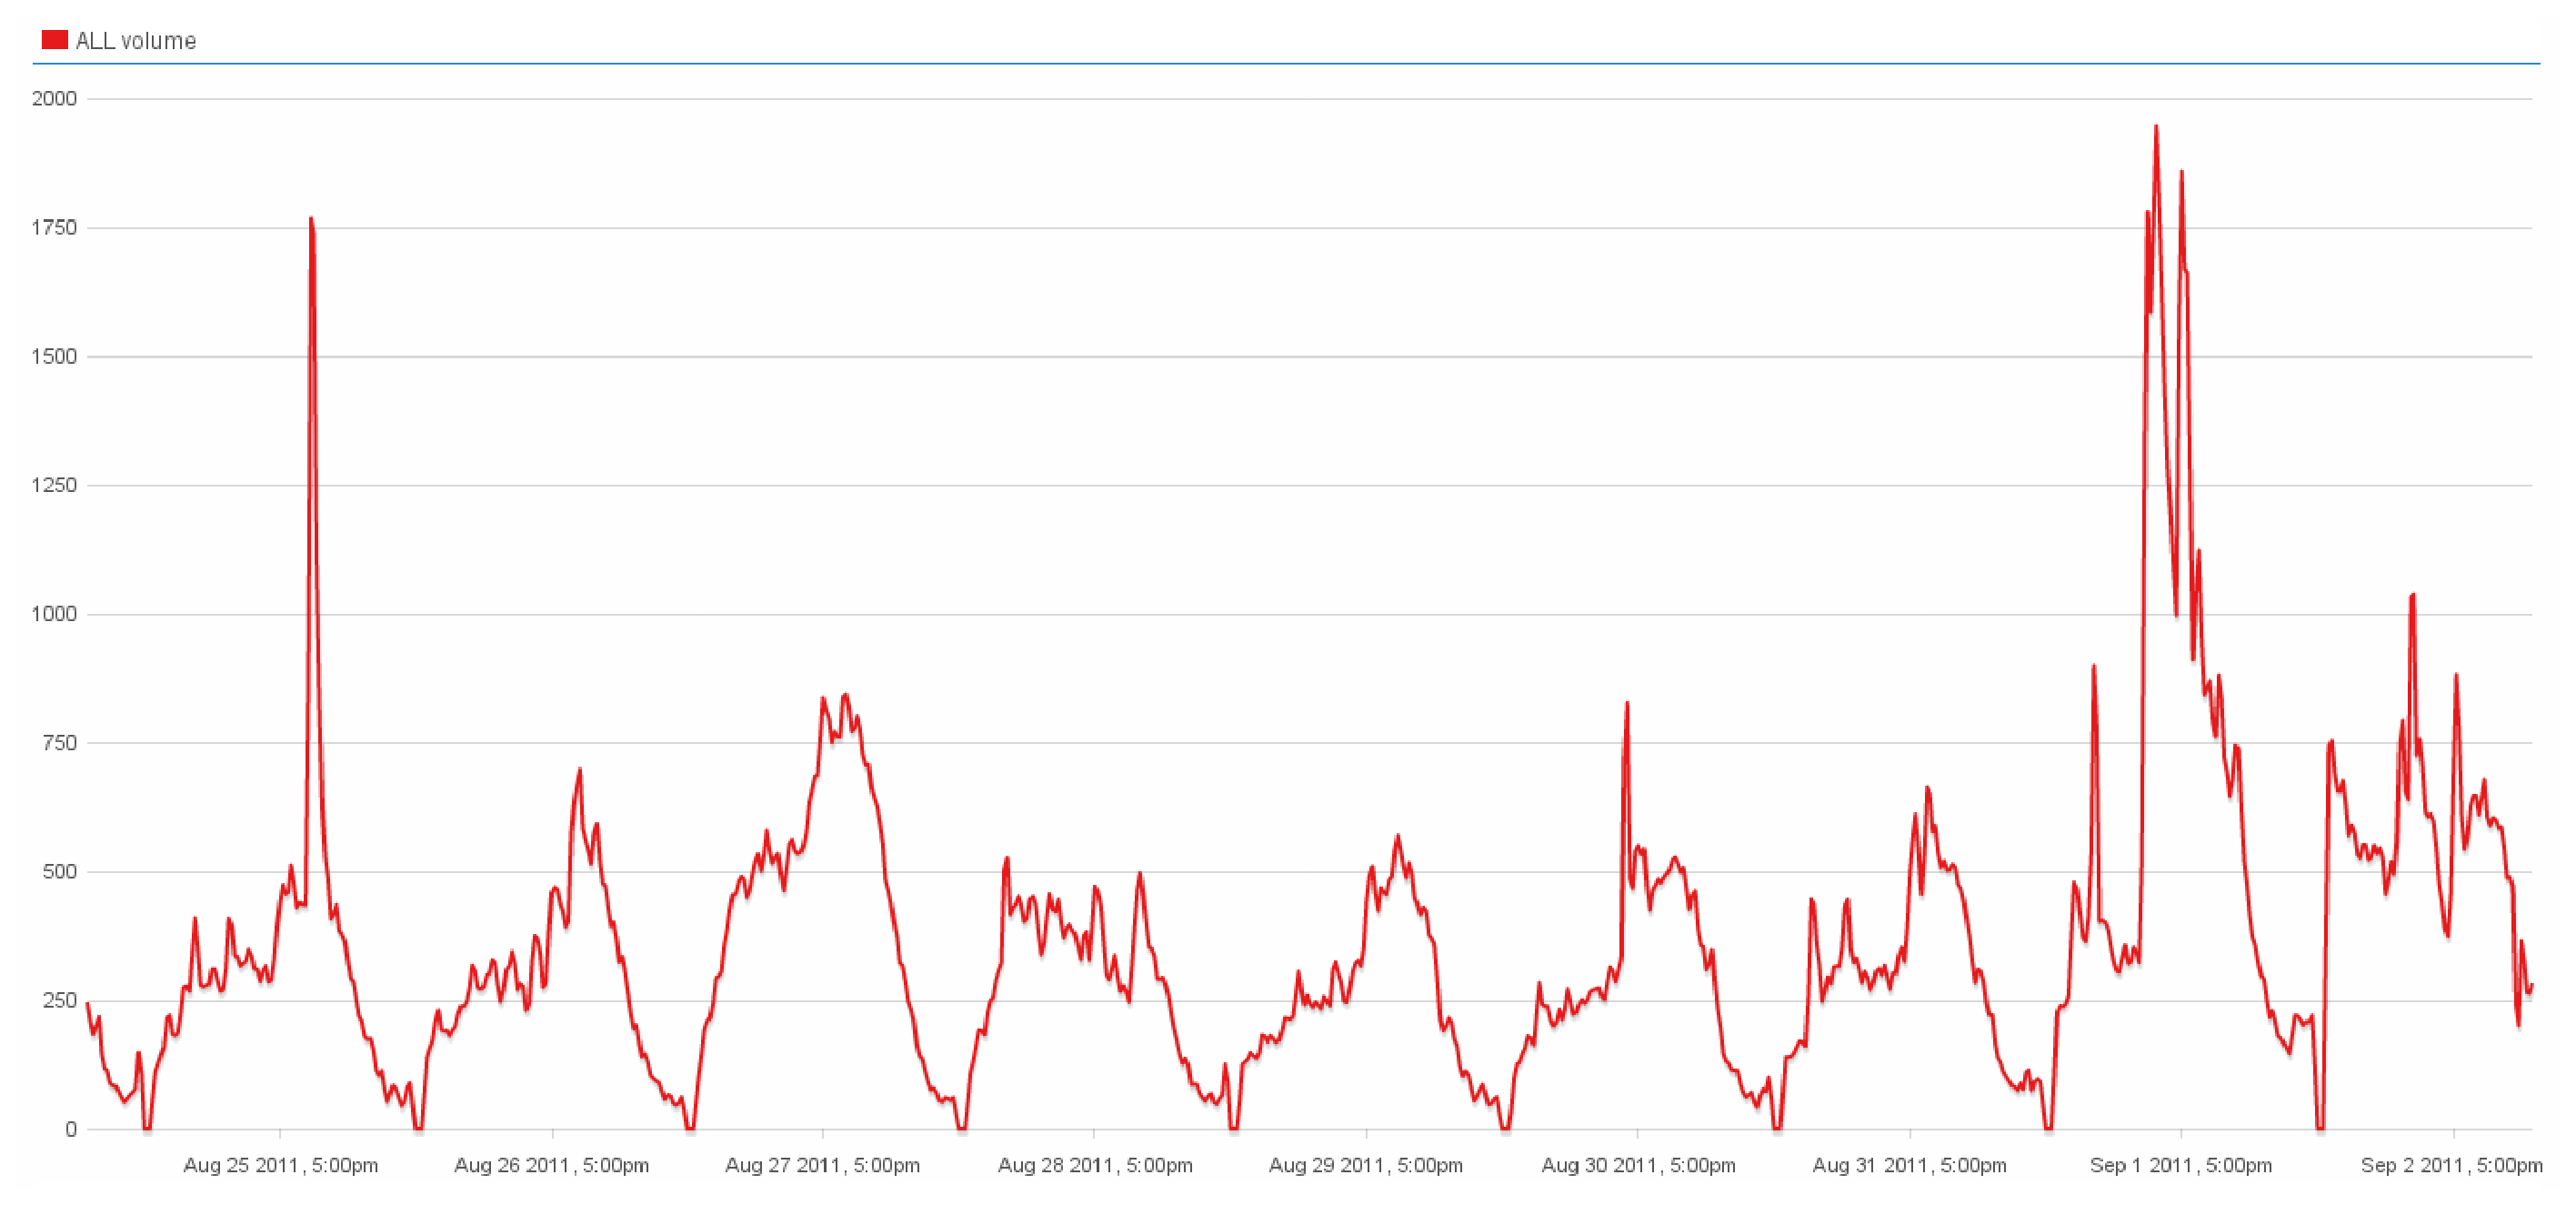
\includegraphics[width=0.8\textwidth]{images/Anomalous_Traffic.eps}
      \captionfonts
      \caption[Anomalous Traffic]{Netflix-related Twitter traffic with two different anomalies.}
      \label{fig:anomalous-traffic}
   \end{center}
\end{figure}

\begin{figure}
   \begin{center}
      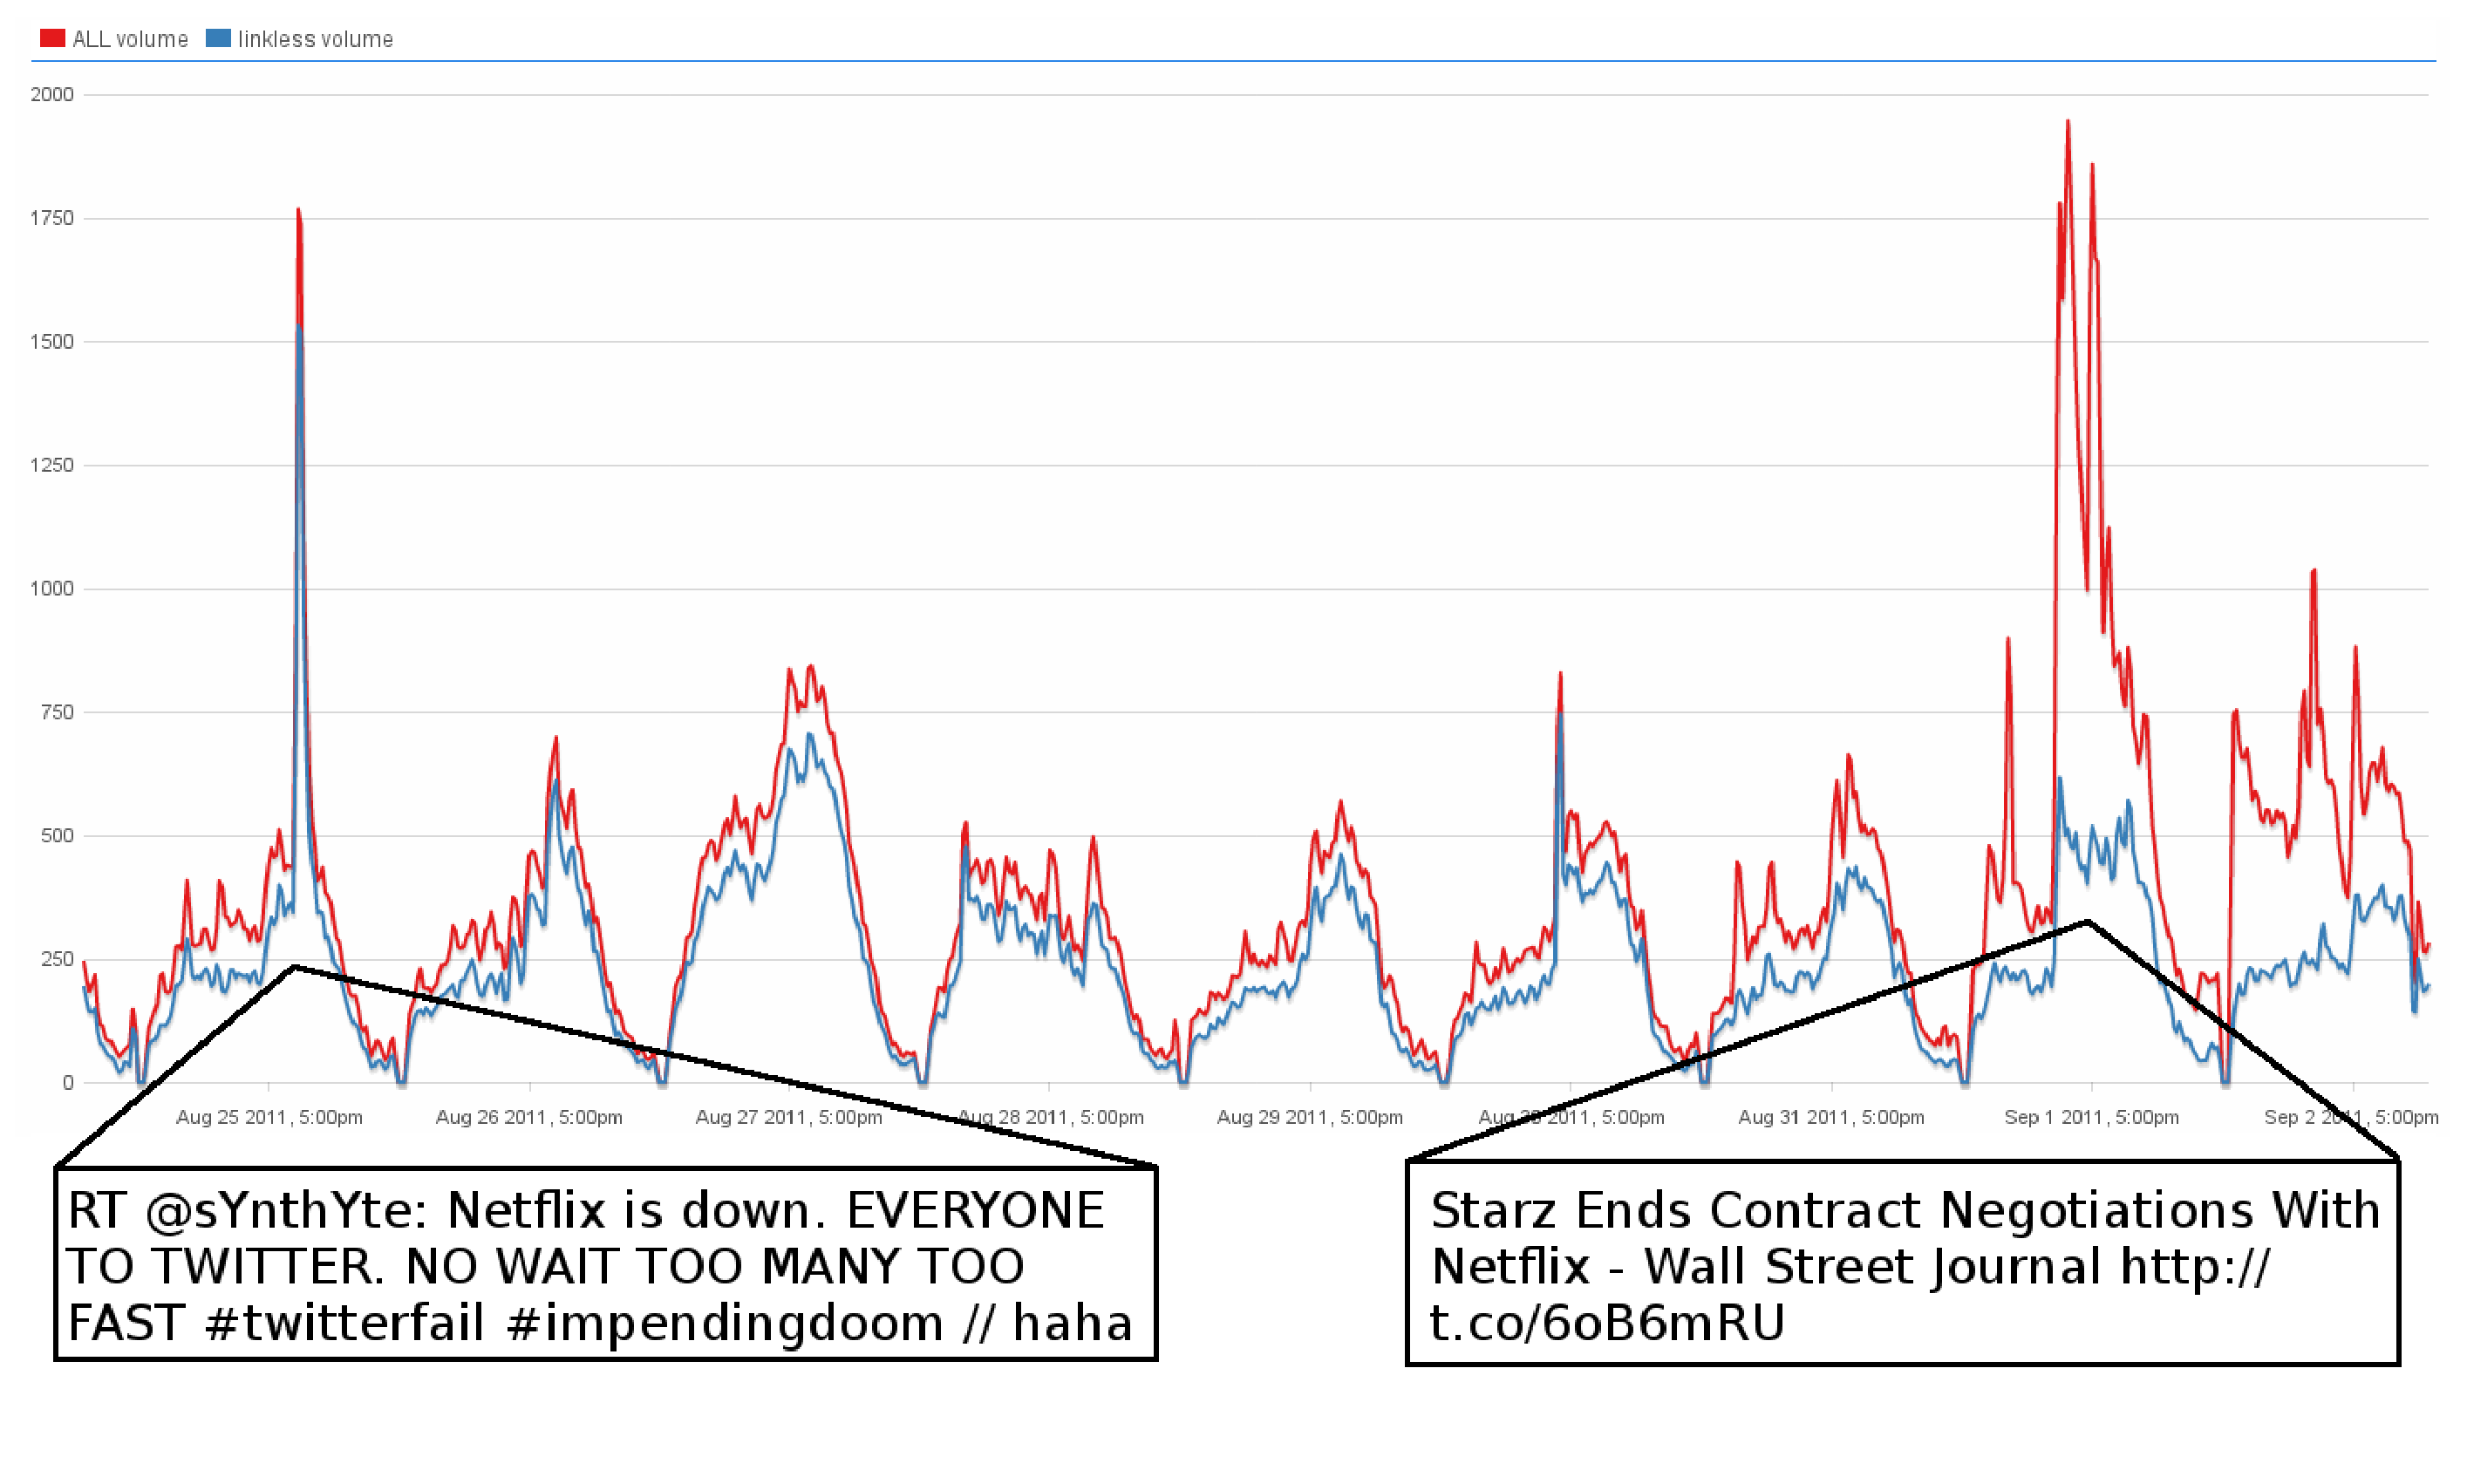
\includegraphics[width=0.8\textwidth]{images/Linkless_Differentiation.eps}
      \captionfonts
      \caption[Linkless Anomalous Traffic]{The same traffic shown in Figure~\ref{fig:anomalous-traffic}, with an additional line showing Netflix-related Twitter traffic that does not contain a URL.}
      \label{fig:linkless-traffic}
   \end{center}
\end{figure}

\begin{figure}
   \begin{center}
      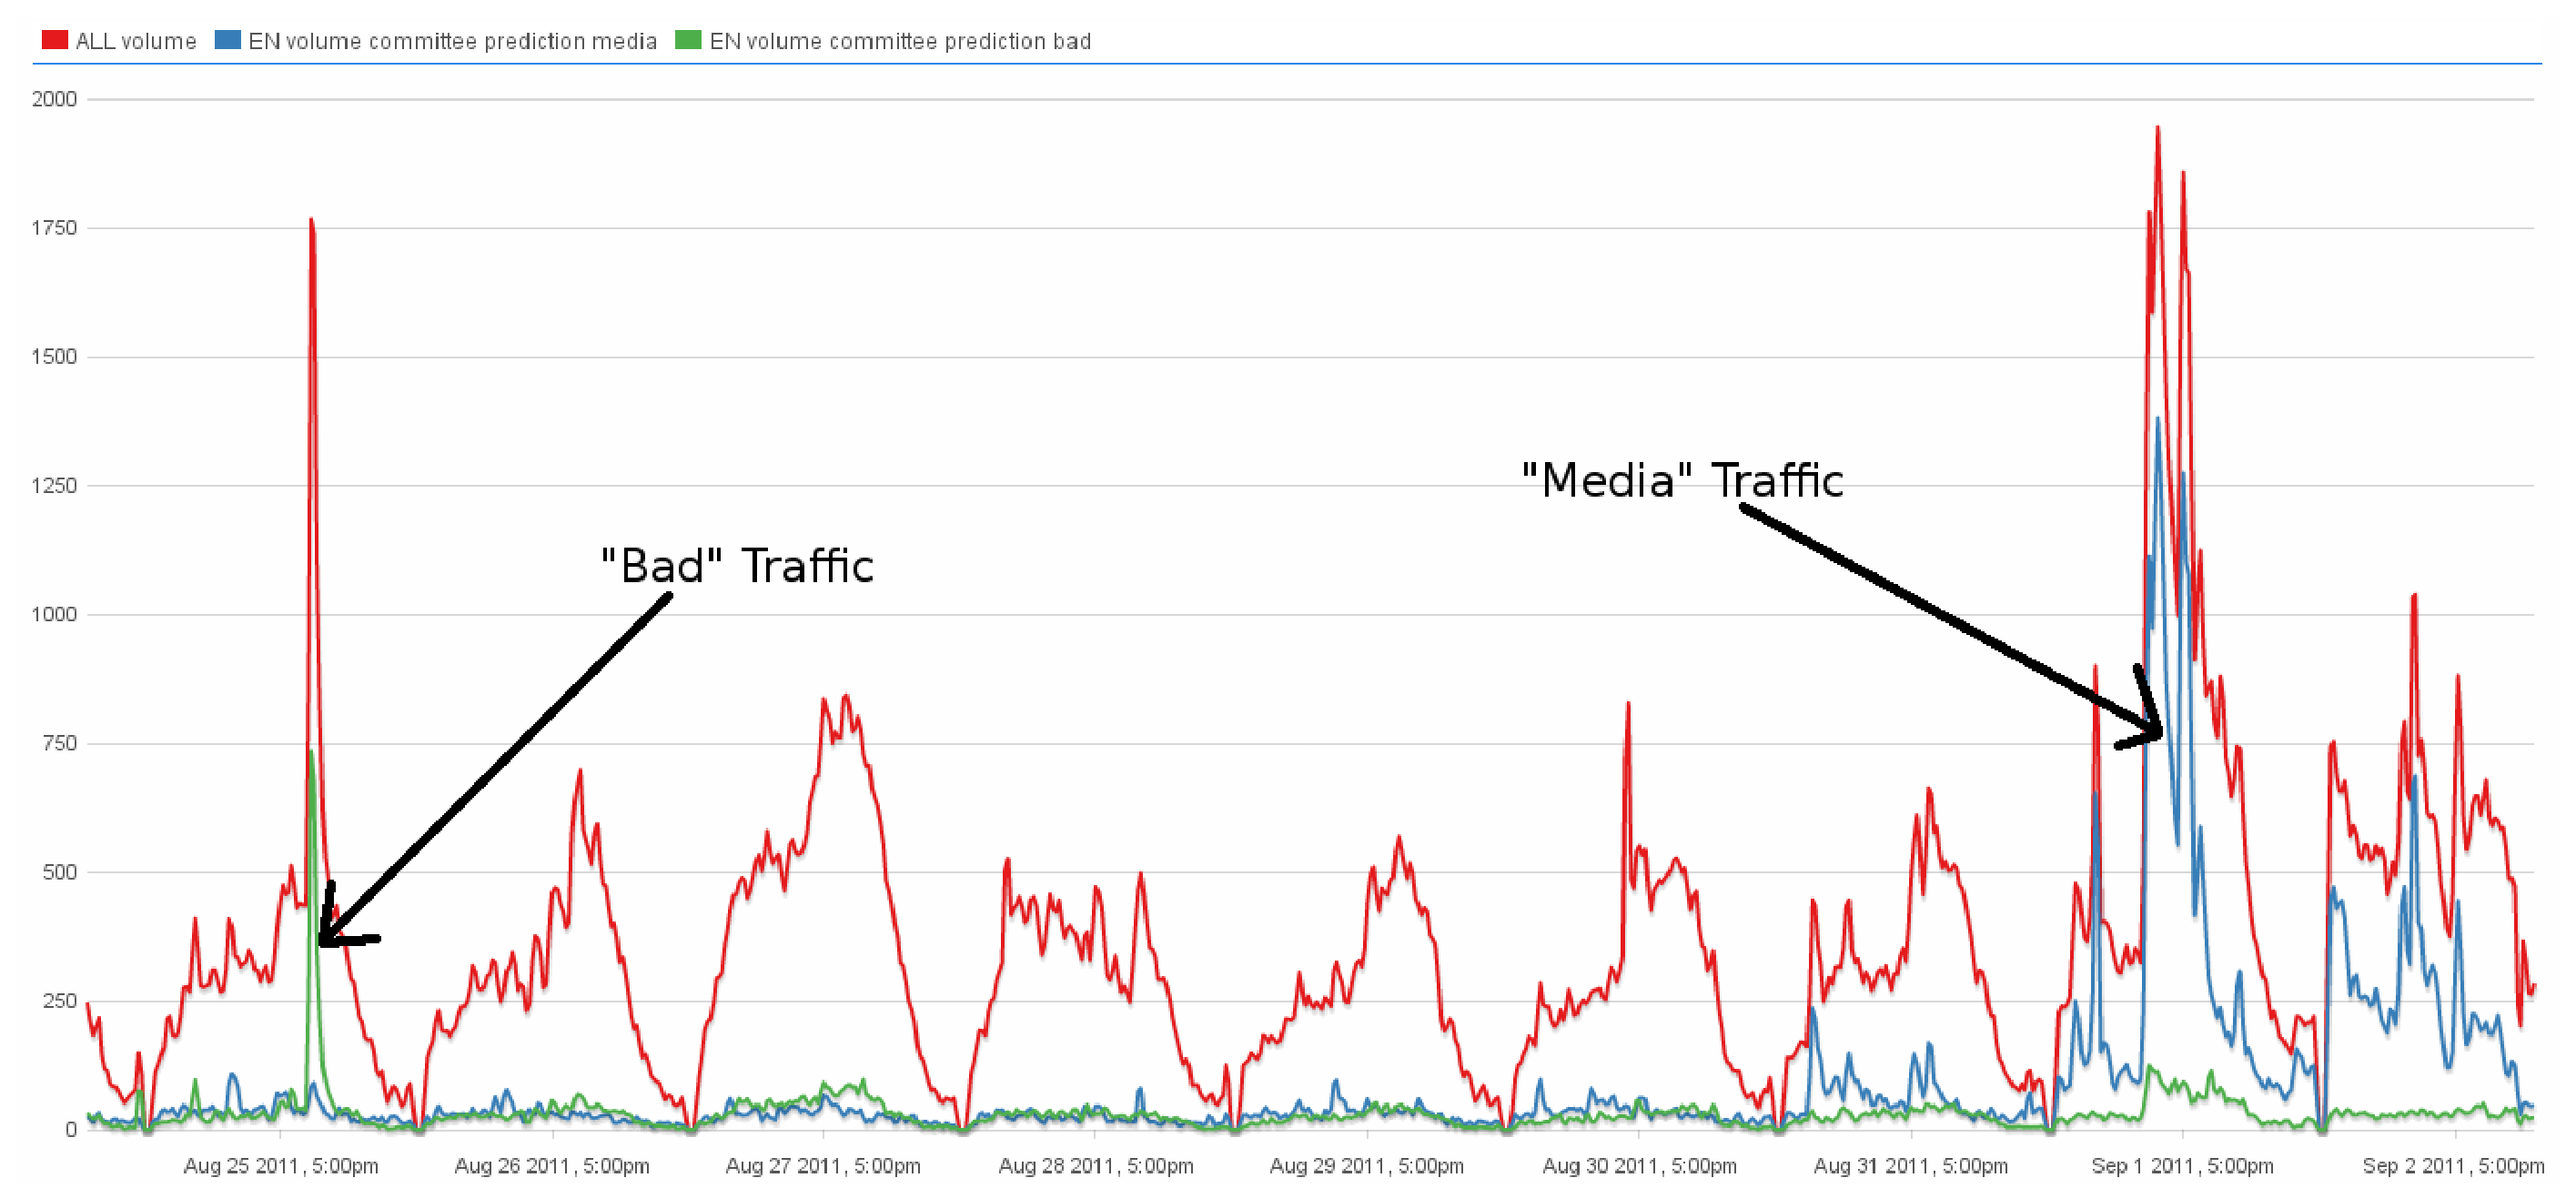
\includegraphics[width=0.8\textwidth]{images/Classified_Traffic.eps}
      \captionfonts
      \caption[Classified Traffic]{The same traffic shown in Figure~\ref{fig:anomalous-traffic}, with two addition lines: the volume of tweets classified as ``Bad'' and the volume of tweets classified as ``Media''.}
      \label{fig:classified-traffic}
   \end{center}
\end{figure}

\section{Classification Roadmap}
\label{class-roadmap}
The steps that SPOONS takes to use classification to detect service outages can be divided into two categories:
prep work and online.

The prep work includes:

\begin{enumerate}
   \item Observe Netflix-related Twitter traffic and observe the different classes that the tweets fall into.
   \item Build a training set biasing anomalous traffic.
   \item Classify incoming tweets.
   \item Group classified tweets according to the type of traffic that class produces.
   \item Establish the best classifiers.
\end{enumerate}

After the off-line prep work is complete, the online analysis can begin:

\begin{enumerate}
   \item Use the best classifiers in an Analysis Pipeline.
   \item Observe the differences between the total traffic and the traffic classified as anomalous.
   \item Declare an outage when the two traffics diverge significantly.
\end{enumerate}

\section{Tweet Classes}
\label{class-tweet-classes}
After observing Netflix-related Twitter traffic, we decided tweets fall into at least one of nine different categories.

\begin{itemize}
  \item \texttt{Media} -- Tweets relating to a media story about Netflix. Typically a link to a news article.
  \item \texttt{Snafu} -- Tweets that talk about a Netflix outage.
  \item \texttt{Complaint} -- Tweets where people are complaining about Netflix.
  \item \texttt{Happy} -- Tweets that expresses the user's joy about Netflix.
  \item \texttt{Neutral} -- Tweets that are just a neutral observation or comment about Netflix.
  \item \texttt{Watching} -- Tweets that gives updates about what the user is currently watching.
  \item \texttt{Response} -- Tweets that are a neutral response to another user in a Netflix-related conversation.
  \item \texttt{Refuse To Rate} -- Tweets that we we refuse to rate entirely (usually tweets that are in a different language than the training set).
  \item \texttt{Undetermined} -- This class does not exist in the wild. It is used during classification as default for all tweets that don't match any other class.
\end{itemize}

Examples of tweets with their corresponding classes are shown in Table~\ref{table:classes}.

\begin{table}
   \begin{center}
      \begin{tabular}{|l|p{12cm}|}
         \hline
            Class & Tweet Example
         \tabularnewline\hline
            \texttt{Media} & \texttt{Netflix Now Available Through Facebook - http://bit.ly/ffpBHH - [Geeky Gadgets]}
         \tabularnewline\hline
            \texttt{Snafu} & \texttt{And netflix is broken. Why is this happening to me.}
         \tabularnewline\hline
            \texttt{Complaint} & \texttt{netflix keeps taking little things i like about the site away...Why?}
         \tabularnewline\hline
            \texttt{Happy} & \texttt{Netflix :)}
         \tabularnewline\hline
            \texttt{Neutral} & \texttt{about to download this netflix free trial}
         \tabularnewline\hline
            \texttt{Watching} & \texttt{Watching Family Guy on Netflix}
         \tabularnewline\hline
            \texttt{Response} & \texttt{@BeehiveBlog  Both good movies.  I think I'll put on the netflix list.}
         \tabularnewline\hline
            \texttt{Refuse To Rate} & \texttt{en serio, QUIERO pagar por algo como Netflix, DEJARME pagar}
         \tabularnewline\hline
      \end{tabular}
   \end{center}
   \caption[Tweet Class Examples]{Examples of the types of tweets that go with each class.}
   \label{table:classes}
\end{table}

\subsection{Tweet Groups}
\label{class-tweet-groups}
Because the goal of SPOONS is to detect anomalous traffic, it is useful to collapse the nine classes into
three different groups that account for the different types of Netflix-related traffic.

\begin{itemize}
  \item \texttt{Media}: Contains only the \texttt{media} class.
  \item \texttt{Bad}: Contains both the \texttt{snafu} and \texttt{complaint} classes.
  \item \texttt{Other/Normal}: Contains all other classes.
\end{itemize}

Figure~\ref{fig:groups} shows the amount of Netflix-related tweets during a Netflix outage and media event.
During normal times, the \texttt{normal} traffic is responsible for the majority of the overall traffic.
However during outage and media events, we see that the \texttt{bad} and \texttt{media} dominate the respective
periods.

\begin{figure}
   \begin{center}
      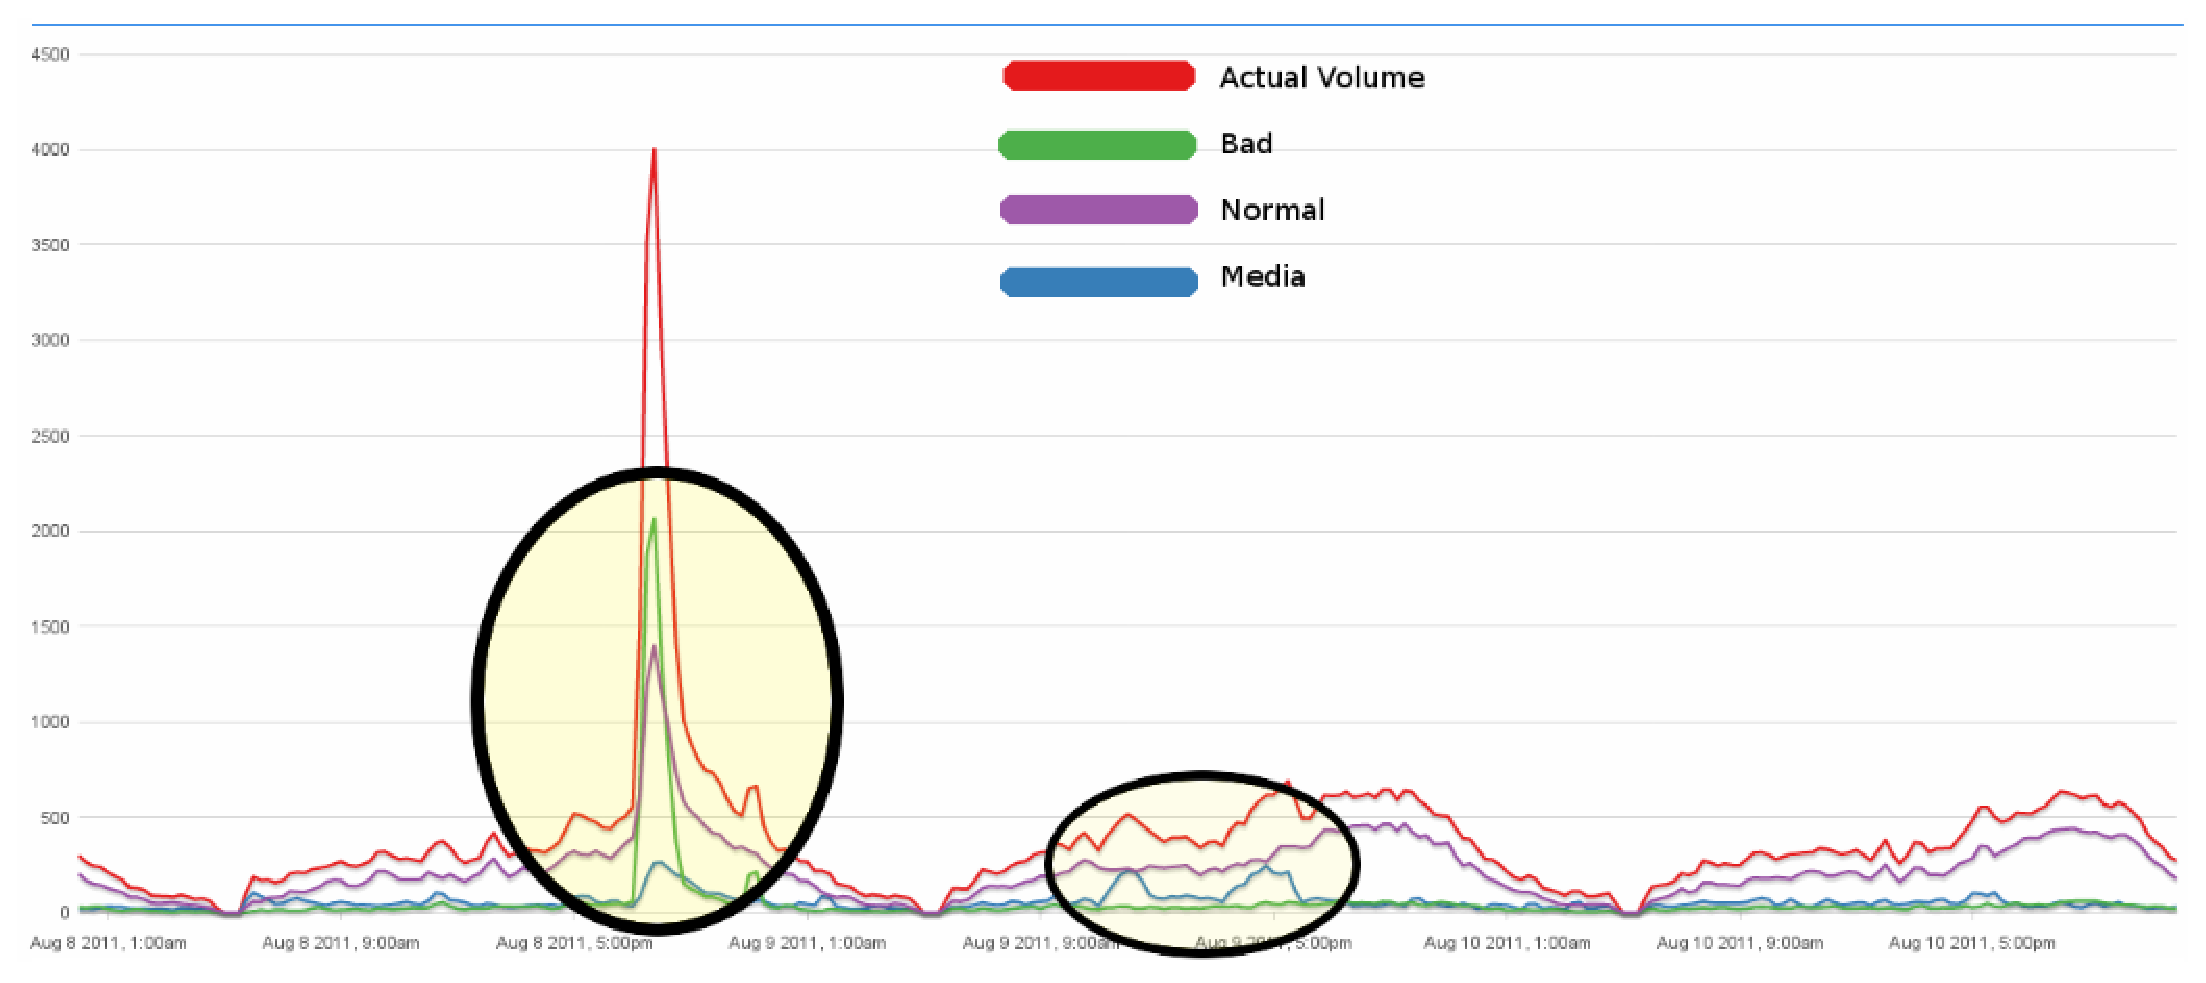
\includegraphics[width=0.8\textwidth]{images/groups.eps}
      \captionfonts
      \caption[SPOONS Groups]{The different volumes for different tweet classes during an outage (left) and media event (right).}
      \label{fig:groups}
   \end{center}
\end{figure}

\section{WEKA Classifiers}
\label{class-weka}
SPOONS uses several classifiers from the WEKA machine learning package\cite{weka}.
All of these classifiers have been discussed in Section~\ref{background-classifiers}.
The WEKA classifiers used are:

\begin{itemize}
   \item Naive Bayes
   \item Bayes Net
   \item J48 (a method of generating a C4.5 decision tree\cite{j48})
   \item K-Nearest Neighbors
   \item SMO (Support Vector Machine trained with Sequential Minimal Optimization\cite{smo})
\end{itemize}

\section{Non-WEKA Classifiers}
\label{class-nonweka}
In addition to the WEKA classifiers, SPOONS uses two classifiers implemented from scratch.
Because of low performance and inflexible API, the WEKA classifiers are being reimplemented.
As of now, only Naive Bayes has been reimplemented. The other classifier implemented from scratch is
a BPNB classifier which is discussed in Section~\ref{background-classifiers-bpnb}.

\section{Text Pre-Processing}
\label{class-processing}
Before the tweets are classified, they are pre-processed. During processing, the text is transformed
to make classification of the text easier. Standard text operations like stemming, stopword removal,
and case normalization; as well as Twitter and Netflix specific operations like hashtag and movie title
recognition are preformed. After the text is processed, it is split into unigrams to be used as features
in the classifiers.

\subsection{Text Filtering}
\label{class-filter}
Before the input text is split into features, it goes through heavy pre-processing.
The text filtering involves normalizing the case, remove extra characters, and replacing special features.

\subsubsection{Link Replacement}
\label{class-filter-link-replacement}
The first step in processing the text is to replace links.
Following a link may provide information about a tweet, however the link text of the link
itself provides no information. The presence of a link, however, can provide information about
a tweet.

\subsubsection{Twitter-Specific Symbols}
\label{class-filter-twitter-symbols}
Tweets often contain several special symbols specific to tweets.

\paragraph{RT.}
\label{class-twitter-symbols-rt}
``RT'' stands for ``re-tweet''. It means that the posted tweet is a repost of
a tweet made by another user. This symbol contains no reference to the original post.
``RT'' usually appears at the beginning of the tweet. For example, after the comedian
Conan O'Brien posted the following tweet:

\begin{center}
   \texttt{If I'm ever a ghost, I hope the person I haunt has Netflix.}
\end{center}

There were hundreds of identical tweets that said:

\begin{center}
   \texttt{RT: If I'm ever a ghost, I hope the person I haunt has Netflix.}
\end{center}

\paragraph{\#.}
\label{class-twitter-symbols-hash}
A ``\#'' (pronounced ``hashtag'') is used to mark keywords or topics.
Users can search for tweets by hashtag and see the collection of tweets supposedly about the
same topic. A hashtag does not have to reference a pre-existing topic.

\paragraph{@.}
\label{class-twitter-symbols-at}
An ``@'' in Twitter, simply pronounced ``at'', is a reference to another Twitter user.
A reference to a user alerts that user about the posted tweet.
For example, the following tweet references my Twitter account.

\begin{center}
   \texttt{Hi there, @eriqaugustine}
\end{center}

\subsubsection{Emoticon Parsing}
\label{class-filter-emoticon}
Emoticons are parsed out and replaced with meta words.
SPOONS emoticon parser was written by Ryan Hanarkis and Allen Dunlea as part of a project for Graduate Artificial Intelligence course.
Emoticons provide a plethora of information about a tweet. Sarcasm aside,
an emoticon can surmise the sentiment of an entire tweet.

\subsubsection{Title Replacement}
\label{class-filter-title}
Because our tweets are always about Netflix, a television show and movie streaming service,
titles are a common occurrence. However, movie and show titles often contain words that can be
detrimental to our analysis. For example, ``Death At A Funeral'' is the title of a movie, but contains
two words that have very negative connotations: ``death'' and ``funeral''.

Without title replacement, the following tweet would be very difficult to classify:

\begin{center}
   \texttt{Death at a Funeral is hilarious!  \#netflix}
\end{center}

However after title replacement, the tweet becomes very easy to classify:

\begin{center}
   \texttt{$\langle$\$title\$$\rangle$ is hilarious!  \#netflix}
\end{center}

SPOONS contains a table that has over 50,000 movie and show titles on Netflix. The titles were gathered
using the Netflix API. On startup, SPOONS builds a trie (prefix tree)\cite{trie} of all of the titles. In this trie titles can
only be split on a word level, not on a character level. Therefore, moving to the next node consumes a single word.
Searching for a title becomes a simple walk down the trie.
If the walk of the trie ends on a terminal node, then a title is found. If not, then the trie is walked again from the beginning
starting at the next word in the tweet. Figure~\ref{fig:title-trie} shows a sample walk in the title trie.

% TODO(eriq): [Lowest Priority] Formalize algorithm with pseudocode.

\begin{figure}
   \begin{center}
      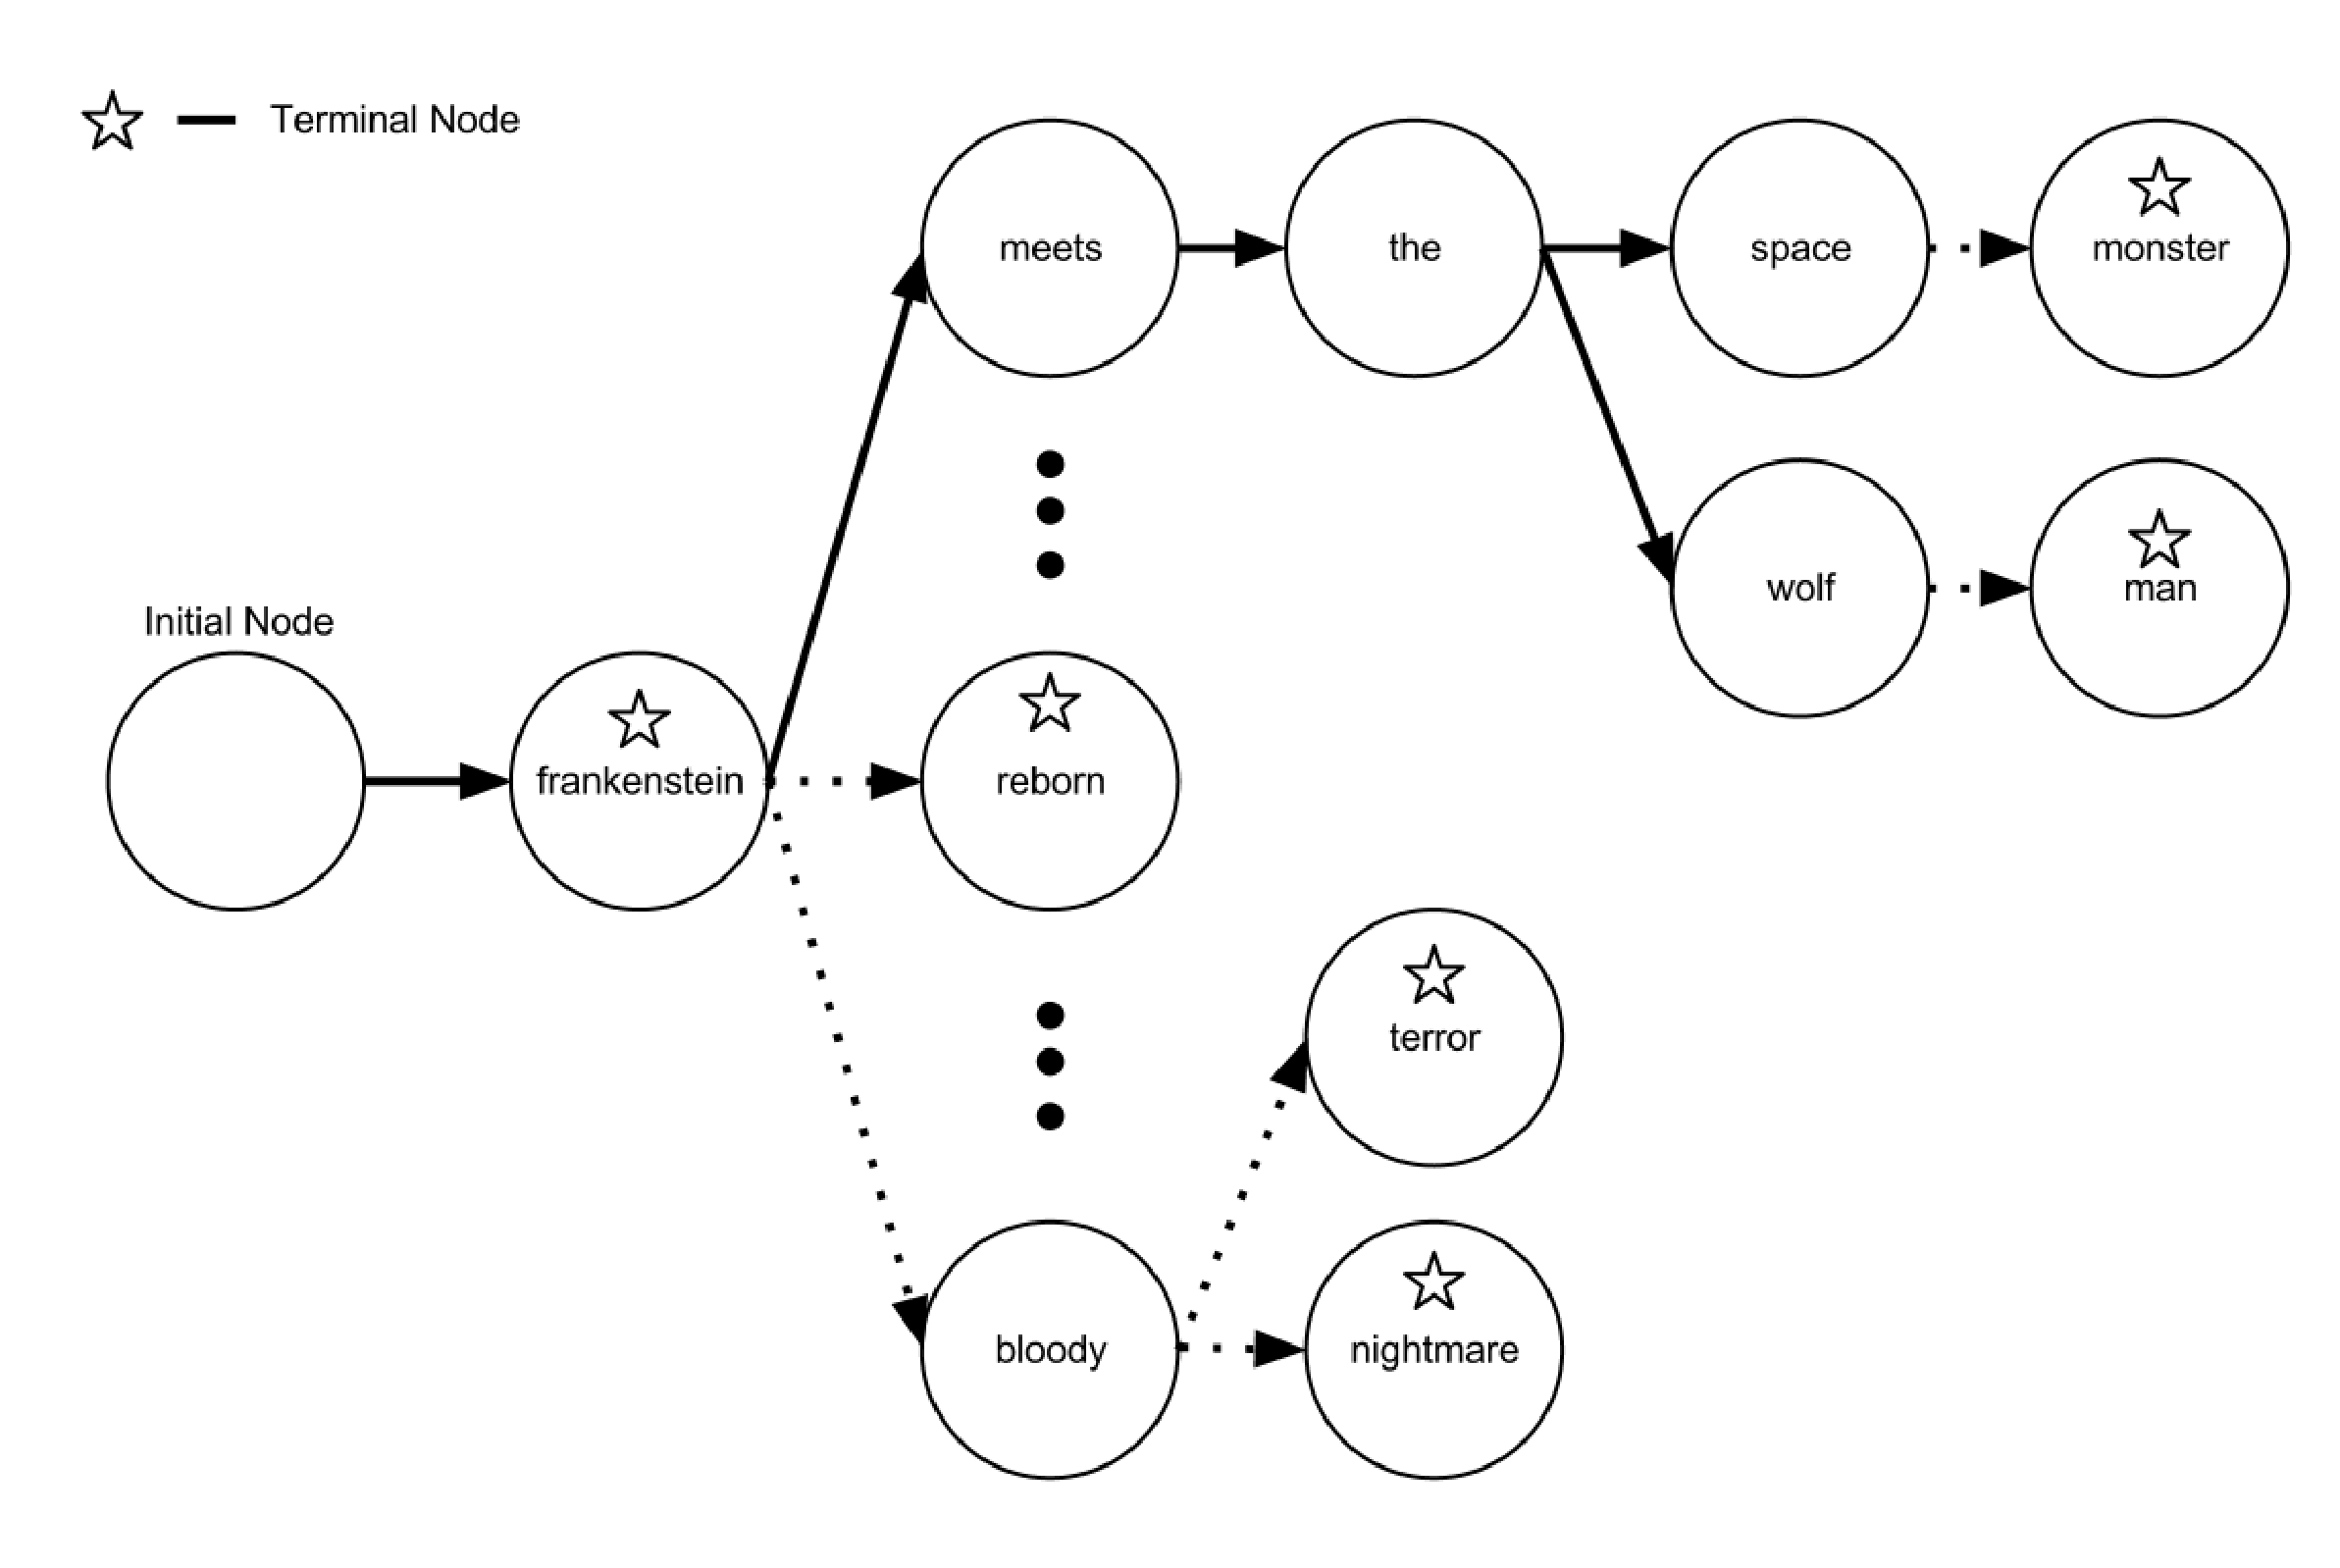
\includegraphics[width=0.8\textwidth]{images/Title_Trie.eps}
      \captionfonts
      \caption[Title Trie Walk]{A sample trie of Frankenstein movie titles. The solid lines show what nodes the search for "Frankenstein Meets The Wolf Man" would traverse.}
      \label{fig:title-trie}
   \end{center}
\end{figure}

\subsubsection{Stemming}
\label{class-filter-stemming}
Stemming finds the root of a word. This allows words to be categorized by their roots which
decreases the number of unique words being evaluated and emphasizes linguistic patterns.
This preprocessor uses Porter's stemmer for the English language \cite{porters}.

\subsubsection{Stop Word Removal}
\label{class-filter-stopword}
Stopwords, or words that carry little or no semantic information, are identified based
on a static table of words mapped to levels. Stopwords are assigned levels which allow
processes to use different sets of stop words. All words less than 3 character are also
automatically considered stop words.

\subsubsection{Punctuation/Non-English Character Removal}
\label{class-filter-noneng}
Removes all punctuation and
characters not in the English alphabet. This simplifies word extraction and
comparison.

\subsubsection{Meta Words}
\label{class-filter-meta}
Below is an overview of meta words that SPOONS recognizes:

\begin{description}
   \item[$\langle$\$title\$$\rangle$] Indicates the presence of a movie or show title.
   \item[$\langle$\$link\$$\rangle$] Indicates the presence of a URL.
   \item[$\langle$\$emote:*\$$\rangle$] Replaces an emoticon.
   \item[$\langle$\$RT\$$\rangle$] Indicates that a tweet is a ``retweet'' (a repeat of another tweet).
   \item[$\langle$\$\#\$$\rangle$] Inserted when a ``hashtag'' is found in a tweet. The original subject of the hashtag is separated off into another word. E.g. ``\#Netflix'' becomes ``$\langle$\$\#\$$\rangle$ Netflix''.
   \item[$\langle$\$@\$$\rangle$] Inserted when a reference to another Twitter user is made. The user that is the subject of the reference is separated off into another word.
\end{description}

\section{Training Set}
\label{class-training-set}

The classifiers were trained on a small set of \textbf{759} tweets which were pulled from from periods of both normal and
anomalous traffic. Each tweet in the training set was manually classified by multiple researchers until consensus
about the classification was reached. Because the goal is anomalous traffic detection, the training set over-samples the
tweets from \texttt{media}, \texttt{snafu}, and \texttt{complaint}: categories. Table~\ref{table:classCounts} documents
the structure of the training set and shows the  number of tweets classified into each of the eight categories.
Tweets were allowed to belong to multiple classes because of posts like, ``\texttt{I love netflix! Watching Law and Order
online!}'', which could be classified as both \texttt{happy} and \texttt{watching}.

See Appendix~\ref{appendix-full-training} for the full training set.

\begin{table}
   \begin{center}
      \begin{tabular}{|l|c|c|c|}
         \hline
         Class  & \# Tweets & Class & \# Tweets
         \tabularnewline\hline
         \texttt{Media} & 103 & \texttt{Neutral} & 66
         \tabularnewline\hline
         \texttt{Outage} & 158  & \texttt{Watching} &  135
         \tabularnewline\hline
         \texttt{Complaint}  & 146 &  \texttt{Response} &  30
         \tabularnewline\hline
         \texttt{Happy}  & 147  & \texttt{Undetermined}  & 48
         \tabularnewline\hline
      \end{tabular}
      \caption[Netflix-related Twitter Traffic]{Overview of the Netflix-related Twitter post training set used to train classifiers in SPOONS.}
      \label{table:classCounts}
   \end{center}
\end{table}

\section{Evaluation}
\label{class-evaluation}
Each classifier is individually evaluated just on its ability to classify tweets against the training set.
Each classifier varies the type of filtering it uses between no filtering and full filtering (every method discussed in Section~\ref{class-filter}).
Table~\ref{table:classifierEvaluationSpace} shows the combinations of classifiers and filters used for the classifier evaluation.
There will be 24 classifier/filtering combinations.

\begin{table}[H]
   \begin{center}
      \begin{tabular}{|l|}
         \hline
            \textbf{Classifiers}
         \tabularnewline\hline
            BayesNetClassifier
         \tabularnewline\hline
            BinaryBayesNetClassifier
         \tabularnewline\hline
            BinaryJ48Classifier
         \tabularnewline\hline
            BinaryKNNClassifier
         \tabularnewline\hline
            BinaryNaiveBayesClassifier
         \tabularnewline\hline
            BinarySMOClassifier
         \tabularnewline\hline
            J48Classifier
         \tabularnewline\hline
            KNNClassifier
         \tabularnewline\hline
            NaiveBayesClassifier
         \tabularnewline\hline
            Non-Weka BPNBClassifier
         \tabularnewline\hline
            Non-Weka NaiveBayesClassifier
         \tabularnewline\hline
            SMOClassifier
         \tabularnewline\hline
      \end{tabular}
      {
         \Huge
         $\times$
      }
      \begin{tabular}{|l|}
         \hline
            \textbf{Filtering}
         \tabularnewline\hline
            None
         \tabularnewline\hline
            Full
         \tabularnewline\hline
      \end{tabular}
      \caption[Classifier Evaluation Combinations]{The cross product of the classifier and filtering will be used to evaluate the classifiers.}
      \label{table:classifierEvaluationSpace}
   \end{center}
\end{table}

\subsection{Confusion Matrices}
\label{class-evaluation-confusion}
The results of the classification evaluation are shown in confusion matrices.
Table~\ref{table:confusionExample} shows the confusion matrix of the Naive Bayes classifier using full filtering as an example.
Down the vertical are the actual classes of the tweets, and across the horizontal are the predicted classes that the classifiers output.
Note that the example shows that this classifier incorrectly classified eight \texttt{media} tweets as another class (seen by looking down the \texttt{media} column),
and misclassified 22 non-media tweets as \texttt{media} (seen by looking across the \texttt{row}).

Overall accuracy for the classifier can be calculated by taking the number of correctly classified tweets (down the diagonal) over the total number of tweets.
Accuracy for a specific classification can be considered two ways: accuracy of classifying tweets \textbf{from} that class and accuracy of classifying \textbf{into} that class.
The accuracy of classifying tweets \textbf{from} a class can be seen by looking down a column.
The number correctly classified tweets (\textbf{bold}) over the total number of tweets in that column.
The accuracy of classifying tweets \textbf{info} a class can be seen using the same method as before, except looking across the class's row instead of its column.

\begin{table}[H]
   \begin{center}
      \scalebox{0.71}{
         \begin{tabular}{|c|c|c|c|c|c|c|c|c|}
         \hline
            \diaghead{\theadfont Diag ColumnmnHead II}{Classified}{Actual} & media & neutral & snafu & watching & response & complaint & refuse to rate & happy \\
         \hline
            media & \textbf{81} & 3 & 0 & 1 & 3 & 0 & 14 & 1 \\
         \hline
            neutral & 0 & \textbf{23} & 3 & 14 & 11 & 11 & 1 & 3 \\
         \hline
            snafu & 0 & 7 & \textbf{81} & 8 & 4 & 55 & 2 & 1 \\
         \hline
            watching & 0 & 26 & 0 & \textbf{82} & 5 & 12 & 0 & 10 \\
         \hline
            response & 2 & 12 & 3 & 6 & \textbf{3} & 1 & 0 & 3 \\
         \hline
            complaint & 1 & 9 & 36 & 9 & 8 & \textbf{77} & 3 & 3 \\
         \hline
            refuse to rate & 5 & 4 & 1 & 2 & 4 & 9 & \textbf{21} & 2 \\
         \hline
            happy & 0 & 18 & 5 & 22 & 5 & 31 & 1 & \textbf{65} \\
         \hline
         \end{tabular}
      }
      \caption[Example Classification Confusion Matrix]{A example confusion matrix for a classifier. The \texttt{undecided} class was removed because there were no tweets in that class.}
      \label{table:confusionExample}
   \end{center}
\end{table}

\subsection{Results}
\label{class-evaluation-results}
Table~\ref{table:classification-summary-uncompressed} shows a summary of the results of the evaluation.
The SMO classifier took the top two spots with a top accuracy of \textbf{.5750}.
This is a decent accuracy, but much of the misclassification occurs between classes that don't matter
as much when trying to identify the different types of classes. For example, it does not matter if
a \texttt{watching} tweet is misclassified as a \texttt{happy} tweet. Both of those classes contribute to
normal background traffic. Table~\ref{table:confusionMisclassification} shows the confusion matrix for the top
ranked classifier (SMO with no filtering). All of the misclassification of the \texttt{other} group that
would become correct classification if the nine classes were compressed to the three groups are \textbf{bold}.
Because of this, the classifiers will be evaluated again, but the different classes
will be compressed into their respective groups before the results are evaluated.

\begin{table}[H]
   \begin{center}
      \scalebox{0.65}{
         \begin{tabular}{|c|c|c|c|c|c|c|c|c|c|}
         \hline
            \diaghead{\theadfont Diag ColumnmnHead II}{Classified}{Actual} & undecided & media & neutral & snafu & watching & response & complaint & refuse to rate & happy \\
         \hline
            undecided& 0 & 0 & 0 & 0 & 0 & 0 & 0 & 0 & 0 \\
         \hline
            media    & 0 & 98 & 0 & 0 & 2 & 2 & 0 & 0 & 1 \\
         \hline
            neutral  & 0 & 3 & 11 & 2 & \textbf{\large 16} & \textbf{\large 7} & 7 & 0 & \textbf{\large 20} \\
         \hline
            snafu    & 0 & 0 & 1 & 87 & 4 & 4 & 41 & 0 & 21 \\
         \hline
            watching & 0 & 2 & \textbf{\large 12} & 3 & 88 & \textbf{\large 5} & 4 & 0 & \textbf{\large 21} \\
         \hline
            response & 0 & 2 & \textbf{\large 5} & 4 & \textbf{\large 7} & 0 & 3 & \textbf{\large 1} & \textbf{\large 8} \\
         \hline
            complaint& 0 & 2 & 5 & 40 & 4 & 1 & 68 & 1 & 25 \\
         \hline
            refuse to rate & 0 & 9 & \textbf{\large 1} & 1 & \textbf{\large 1} & \textbf{\large 1} & 0 & 18 & \textbf{\large 17} \\
         \hline
            happy    & 0 & 1 & \textbf{\large 9} & 3 & \textbf{\large 13} & \textbf{\large 6} & 8 & 0 & 107 \\
         \hline
         \end{tabular}
      }
      \caption[Uncompressed Misclassification Example]{The SMO results with no filtering. Every misclassification that would map to the \texttt{other} group is bold.}
      \label{table:confusionMisclassification}
   \end{center}
\end{table}

\subsection{Compressed Results}
\label{class-evaluation-compressed-results}
Table~\ref{table:classification-summary-compressed} shows a summary of the compressed results.
After the classes have been compressed, the SMO classifier is still on top but now with a best accuracy
of \textbf{.8583}. Compressing the classes into groups greatly increases the accuracy of the classifiers.

It is important to note that not only is overall accuracy important, but also the precision for the \texttt{snafu} group.
If SPOONS is stable capturing and classifying anomalous traffic, then when there is a spike then it will be visible.
However if there are too many false positives, then a spike cannot be trusted. Recall affects the size of a spike, but precision
affects the shape of the spike.

Table~\ref{table:confusionPrecisionRecall} shows an example of a compressed classification confusion matrix.
The \textbf{bold} cells shows \texttt{snafu} tweets that were misclassified as other groups. Our number one priority is to minimize these cells.
These cells represent the precision of the classifier for the \texttt{snafu} group (lower numbers generate higher precision). 
The \emph{italics} cells shows tweets that were incorrectly classified as \texttt{snafu}. Although we also want to minimize these
cells, they are not as important as the \textbf{bold} cells.

\begin{table}[H]
   \begin{center}
      \scalebox{0.62}{
         \begin{tabular}{|c|c|c|c|}
         \hline
            \diaghead{\theadfont Diag ColumnmnHead II}{Classified}{Actual} & media & snafu & other \\
         \hline
            media & 95 & \textbf{0} & 8 \\
         \hline
            snafu & \emph{1} & 252& \emph{51} \\
         \hline
            other & 13 & \textbf{77} & 336\\
         \hline
         \end{tabular}
      }
      \caption[Misclassified Snafu]{A sample compressed classification confusion matrix showing misclassified \texttt{snafu} tweets.}
      \label{table:confusionPrecisionRecall}
   \end{center}
\end{table}

Full results for both the uncompressed and compressed evaluation can be found in Appendix~\ref{appendix-full-classifier}.

\begin{center}
   \begin{longtable}{|l|l|l|c|c|c|}
      \hline
         Classifier & Text Filter & Accuracy
      \tabularnewline\hline
         \textbf{SMOClassifier} & \textbf{None} & \textbf{0.5726}
      \tabularnewline\hline
         SMOClassifier & Full & 0.5618
      \tabularnewline\hline
         BinaryNaiveBayesClassifier & None & 0.5606
      \tabularnewline\hline
         NaiveBayesClassifier & None & 0.5462
      \tabularnewline\hline
         J48Classifier & Full & 0.5414
      \tabularnewline\hline
         BinaryNaiveBayesClassifier & Full & 0.5414
      \tabularnewline\hline
         J48Classifier & None & 0.5294
      \tabularnewline\hline
         Non-Weka BPNBClassifier & Full & 0.5210
      \tabularnewline\hline
         NaiveBayesClassifier & Full & 0.5198
      \tabularnewline\hline
         BinarySMOClassifier & Full & 0.5174
      \tabularnewline\hline
         BinarySMOClassifier & None & 0.5126
      \tabularnewline\hline
         BinaryBayesNetClassifier & Full & 0.4982
      \tabularnewline\hline
         BayesNetClassifier & None & 0.4970
      \tabularnewline\hline
         Non-Weka BPNBClassifier & None & 0.4958
      \tabularnewline\hline
         BinaryBayesNetClassifier & None & 0.4958
      \tabularnewline\hline
         BayesNetClassifier & Full & 0.4646
      \tabularnewline\hline
         BinaryJ48Classifier & Full & 0.4622
      \tabularnewline\hline
         BinaryJ48Classifier & None & 0.4514
      \tabularnewline\hline
         BinaryKNNClassifier & None & 0.4406
      \tabularnewline\hline
         KNNClassifier & None & 0.4382
      \tabularnewline\hline
         Non-Weka NaiveBayesClassifier & Full & 0.4082
      \tabularnewline\hline
         KNNClassifier & Full & 0.3854
      \tabularnewline\hline
         BinaryKNNClassifier & Full & 0.3830
      \tabularnewline\hline
         Non-Weka NaiveBayesClassifier & None & 0.3553
      \tabularnewline\hline
      \caption[Uncompressed Classification Results Summary]{Uncompressed Classification Results Summary}
      \label{table:classification-summary-uncompressed}
   \end{longtable}
\end{center}

\begin{center}
   \begin{longtable}{|l|l|l|c|c|c|}
      \hline
         Classifier & Text Filter & Accuracy
      \tabularnewline\hline
         \textbf{SMOClassifier} & \textbf{Full} & \textbf{0.8583}
      \tabularnewline\hline
         SMOClassifier & None & 0.8499
      \tabularnewline\hline
         Non-Weka BPNBClassifier & Full & 0.8271
      \tabularnewline\hline
         BinarySMOClassifier & None & 0.8259
      \tabularnewline\hline
         BinarySMOClassifier & Full & 0.8235
      \tabularnewline\hline
         BinaryNaiveBayesClassifier & None & 0.8235
      \tabularnewline\hline
         BinaryNaiveBayesClassifier & Full & 0.8199
      \tabularnewline\hline
         NaiveBayesClassifier & None & 0.8175
      \tabularnewline\hline
         Non-Weka BPNBClassifier & None & 0.8151
      \tabularnewline\hline
         J48Classifier & Full & 0.8091
      \tabularnewline\hline
         NaiveBayesClassifier & Full & 0.8079
      \tabularnewline\hline
         BinaryKNNClassifier & None & 0.7899
      \tabularnewline\hline
         J48Classifier & None & 0.7887
      \tabularnewline\hline
         KNNClassifier & None & 0.7863
      \tabularnewline\hline
         KNNClassifier & Full & 0.7623
      \tabularnewline\hline
         Non-Weka NaiveBayesClassifier & Full & 0.7611
      \tabularnewline\hline
         BinaryKNNClassifier & Full & 0.7575
      \tabularnewline\hline
         Non-Weka NaiveBayesClassifier & None & 0.7263
      \tabularnewline\hline
         BayesNetClassifier & None & 0.7263
      \tabularnewline\hline
         BinaryJ48Classifier & None & 0.6879
      \tabularnewline\hline
         BinaryBayesNetClassifier & Full & 0.6855
      \tabularnewline\hline
         BinaryBayesNetClassifier & None & 0.6819
      \tabularnewline\hline
         BinaryJ48Classifier & Full & 0.6759
      \tabularnewline\hline
         BayesNetClassifier & Full & 0.6603
      \tabularnewline\hline
      \caption[Compressed Classification Results Summary]{Compressed Classification Results Summary}
      \label{table:classification-summary-compressed}
   \end{longtable}
\end{center}



\chapter{Outage Detection}
\label{outage-detection}

\section{Ground Truth}
\label{outage-detection-truth}
Netflix has provided us with a list of outages that occurred between March 14, 2011 and January 30, 2012.
This list is not comprehensive and some of the times are questionable. Some of the outages contained in the list
are internal outages that did not affect their streaming service. These outages generated no signal on Twitter.
Therefore, errors of omission could fall into one of two categories: true failures to recognize outages, and uncatchable
outages. Regardless, we use this as our base truth about all of the Netflix outages in that time period.

\section{Success Metrics}
\label{outage-detection-metrics}
The accuracy of outage detection is measured using three metrics: Recall, Precision, and F$_{0.5}$.

The following definitions are used to calculate the accuracy metrics:
\begin{itemize}
   \item tp --- True Positive. Any intersection between a reported outage range and a detected outage range.
   \item fp --- False Positive. Any detected outage that has no intersection in the events reported by Netflix.
   \item fn --- False Negative. An alert that has no intersection on an event reported by Netflix is a false negative.
\end{itemize}

\subsection{Recall}
The percent of the reported events that were caught.
\begin{center}
   $Recall = \frac{tp}{tp + fn}$
\end{center}

\subsection{Precision}
The percent of the alerts generated that occurred during an outage event.
Netflix has specified that a precision of 0.5 is an acceptable amount of noise.
\begin{center}
   $Precision = \frac{tp}{tp + fp}$
\end{center}

\subsection{F$_{0.5}$ Score}
A harmonic mean between recall and precision. The standard F$_{1}$ score evenly weighs precision and recall.
F$_{0.5}$ weighs precision more than recall. Precision is being weighed more heavily than recall because
every alert that SPOONS generates would require the intervention of a Netflix engineer. Generating too many
false positives would just cause SPOONS to be ignored.
\begin{center}
   $F_{\beta} = (1 + \beta^{2}) \cdot \frac{precision \cdot recall}{\beta^{2} \cdot precision + recall}$
\end{center}
\begin{center}
   $F_{0.5} = 1.25 \cdot \frac{precision \cdot recall}{.25 \cdot precision + recall}$
\end{center}

\section{Outage Detection Pipeline}
\label{outage-detection-pipeline}

\subsection{Processors}
\label{outage-detection-processors}
TODO(eriq)

\subsection{Modeler}
\label{outage-detection-modeler}
TODO(eriq)

\subsection{Monitors}
\label{outage-detection-monitors}
SPOONS uses a number of Monitors that use different methods to try and detect anomalies in the traffic.
This section will describe each Monitor used.
Each Monitor described will have two tables describing the parameters that can tune this Monitor and
the inputs that the Monitor takes. In addition, each Monitor will have a text description along with it.

\subsubsection{Baseline Monitor}
\label{outage-detection-monitors-Baseline}
\begin{table}[H]
   \begin{center}
      \begin{tabular}{|c|c|c|}
         \hline
            Parameter & Description & Restrictions \\
         \hline
            B & Baseline & $ B > 0 $\\
         \hline
      \end{tabular}
   \end{center}
\end{table}

\begin{table}[H]
   \begin{center}
      \begin{tabular}{|c|c|c|}
         \hline
            Input & Description & Restrictions \\
         \hline
            X & Any time series & - \\
         \hline
      \end{tabular}
   \end{center}
\end{table}

The Baseline Monitor looks for any value above B, and counts that as anomalous.
Ironically, because of its naivety it also provides a decent baseline for the Monitors.

\subsubsection{Windowed Standard Deviation Monitor}
\label{outage-detection-monitors-WindowStdDev}
\begin{table}[H]
   \begin{center}
      \begin{tabular}{|c|c|c|}
         \hline
            Parameter & Description & Restrictions \\
         \hline
            W & Window Size & $ W > 0 $\\
         \hline
            L & Lower Threshold & $L > 0 $\\
         \hline
            U & Upper Threshold & $U >= L $\\
         \hline
      \end{tabular}
   \end{center}
\end{table}

\begin{table}[H]
   \begin{center}
      \begin{tabular}{|c|c|c|}
         \hline
            Input & Description & Restrictions \\
         \hline
            X & Any time series & - \\
         \hline
      \end{tabular}
   \end{center}
\end{table}

The Windowed Standard Deviation Monitor is one of the simplest Monitors. This Monitor takes a $W$ sized window worth of data
and uses the standard deviation of the window to find outliers. Any outliers more than $L$ are considered anomalies and counts towards
an alert, but are still included in the windowed standard deviation calculation. Any value above $U$ is considered an anomaly, but not included
in the standard deviation calculation. The reason for this is that values above $U$ are extreme outliers.

The calculation for the standard deviation, is based off of an iterative approach described in Knuth's ``The Art of Computer Programming'' is used \cite{Knuth}.
Because Knuth's approach was iterative, it could be modified it to calculate for a range of values in an on-line fashion.

Adding the $k$th value, $x$, to the window:
\begin{eqnarray*}
   \lefteqn{Mean(k) = }\\
   && \frac{Mean(k - 1) * (k - 1) - Mean(k - W) + x}{k}
\end{eqnarray*}
$$
   V(k) = (x - Mean(k)) * (x - Mean(k - 1))
$$
$$
   T(k) = T(k - 1) - V(k - W) + V(k)
$$
$$
   WindowStdDev(k) = \sqrt{\frac{T(K))}{k - 1}}
$$

\subsubsection{Weekly Offset Windowed Standard Deviation Monitor}
\label{outage-detection-monitors-WeeklyWindowStdDev}
\begin{table}[H]
   \begin{center}
      \begin{tabular}{|c|c|c|}
         \hline
            Parameter & Description & Restrictions \\
         \hline
            W & Window Size & $ W > 0 $\\
         \hline
            L & Lower Threshold & $L > 0 $\\
         \hline 
            U & Upper Threshold & $U >= L $\\
         \hline 
      \end{tabular}
   \end{center}
\end{table}

\begin{table}[H]
   \begin{center}
      \begin{tabular}{|c|c|c|}
         \hline
            Input & Description & Restrictions \\
         \hline
            X & Any time series & - \\
         \hline
      \end{tabular}
   \end{center}
\end{table}

The Weekly Offset Window Standard Deviation Monitor leverages the periodicity of tweet volume.
Not only is there a daily pattern in traffic, but there is also an even stronger weekly pattern.
The stronger weekly pattern makes sense if one views Netflix-related Twitter traffic as a representative for the number of
people currently watching Netflix. People tend to have pattern that they follow, and people are more available
on different days of the week (especially Friday).

This Monitor holds a windowed standard deviation for every 30 minute time period with 15 minute offsets
for every week. Therefore, values are not compared to the other values around it, but to expected values from
previous weeks. This Monitor uses the same tactics as the Windows Standard Deviation Monitor for counting anomalies.

\subsubsection{Mean Squared Error Monitor}
\label{outage-detection-monitors-MSE}
\begin{table}[H]
   \begin{center}
      \begin{tabular}{|c|c|c|}
         \hline
            Parameter & Description & Restrictions \\
         \hline
            W & Window Size & $ W > 0 $\\
         \hline
            T & Threshold & $ T > 0 $\\
         \hline
      \end{tabular}
   \end{center}
\end{table}

\begin{table}[H]
   \begin{center}
      \begin{tabular}{|c|c|c|}
         \hline
            Input & Description & Restrictions \\
         \hline
            X & The expected time series & - \\
         \hline
            Y & The actual time series & $ Y(k) < X(k) $ \\
         \hline
      \end{tabular}
   \end{center}
\end{table}

The Mean square Error Monitor keeps a windowed mean squared error (MSE). This Monitor requires two sets of input, a set
of expected values and a set of actual values. Any value that causes the MSE to go above a certain threshold, $T$,
counts towards an anomaly.

Adding the $k$th value to the window MSE:
$$
   V(k) = (X(k) - Y(k))^{2}
$$
\begin{eqnarray*}
   \lefteqn{MSE(k) = }\\
   && \frac{MSE(k - 1) * (k - 1) - V(k - W) + V(k)}{k}
\end{eqnarray*}

\subsubsection{Ratio Monitor}
\label{outage-detection-monitors-Ratio}
\begin{table}[H]
   \begin{center}
      \begin{tabular}{|c|c|c|}
         \hline
            Parameter & Description & Restrictions \\
         \hline
            T & Threshold & $ 0 < T < 1 $\\
         \hline
      \end{tabular}
   \end{center}
\end{table}

\begin{table}[H]
   \begin{center}
      \begin{tabular}{|c|c|c|}
         \hline
            Input & Description & Restrictions \\
         \hline
            X & The expected time series & - \\
         \hline
            Y & The actual time series & $ Y(k) < X(k) $\\
         \hline
      \end{tabular}
   \end{center}
\end{table}

The Ratio Monitor takes the ratio of the actual value over the expected value for every time period.
Whenever the ratio dips under the threshold $T$, then that period counts towards an anomaly.
This Monitor may seem simple, but the real challenge lies in picking a proper $X$ and $Y$.
If a good approximating time series can be chosen, then the Monitor can be very successful.

\subsubsection{Class Correlation Monitor}
\label{outage-detection-monitors-Correlation}
\begin{table}[H]
   \begin{center}
      \begin{tabular}{|c|c|c|}
         \hline
            Parameter & Description & Restrictions \\
         \hline
            W & Window Size & $ W > 0 $\\
         \hline
            T & Threshold & $ -1 < T < 1 $\\
         \hline
      \end{tabular}
   \end{center}
\end{table}

\begin{table}[H]
   \begin{center}
      \begin{tabular}{|c|c|c|}
         \hline
            Input & Description & Restrictions \\
         \hline
            X & The expected time series & - \\
         \hline
            Y & The actual time series & $ Y(k) < X(k) $\\
         \hline
      \end{tabular}
   \end{center}
\end{table}

The Correlation Monitor takes the Pearson Correlation between $X$ and $Y$ for a running window of size $W$.
Pearson Correlation is used because of its ability to catch the linear correlation between two time series within
a normalized range.

For performance reasons SPOONS uses an approximation of Pearson Correlation which uses the windowed standard deviation approach
described in Section~\ref{outage-detection-monitors-WindowStdDev}.

Adding the $k$th value, to the window:
$$
   Let \bar{X} be the windowed mean of X.
$$
$$
   Let \bar{Y} be the windowed mean of Y.
$$
\begin{eqnarray*}
   \lefteqn{T(k) = }\\
   && T(k - 1) + (X(k) * Y(k)) - (X(k - W) * Y(k -W))
\end{eqnarray*}
\begin{eqnarray*}
   \lefteqn{Pearson(k) = }\\
   && \frac{T(k) - (W * \bar{X} * \bar{Y})}{(W - 1) * WindowStdDev(X) * WindowStdDev(Y)}
\end{eqnarray*}

\section{Results}
\label{outage-detection-results}
TODO(eriq): Numbers
Full = Appendix~\ref{appendix-full-outage-detection}.

{
   \footnotesize
   \setlength{\LTleft}{-20cm plus -1fill}
   \setlength{\LTright}{\LTleft}
   \begin{longtable}{|l|l|l|c|c|c|c|c|}
      \hline
         Monitor & Classifier & Filtering & Precision & Recall & F$_{0.5}$ Score & Coverage & Adjusted Score
      \tabularnewline\hline
      \endhead
         \textbf{WeeklyWindowStdDev} & \textbf{SMO} & \textbf{Full} & \textbf{0.9583} & \textbf{0.4510} & \textbf{0.6970} & \textbf{0.2890} & \textbf{0.4956}
      \tabularnewline\hline
         WeeklyWindowStdDev & BinaryNaiveBayes & Full & 0.8846 & 0.4510 & 0.6699 & 0.2618 & 0.4945
      \tabularnewline\hline
         WeeklyWindowStdDev & J48 & Full & 0.9545 & 0.4118 & 0.6632 & 0.2583 & 0.4919
      \tabularnewline\hline
         WeeklyWindowStdDev & BPNB & None & 0.9667 & 0.4265 & 0.6797 & 0.2894 & 0.4830
      \tabularnewline\hline
         WeeklyWindowStdDev & BinarySMO & None & 0.9588 & 0.4559 & 0.7010 & 0.3116 & 0.4825
      \tabularnewline\hline
         WeeklyWindowStdDev & SMO & None & 0.9659 & 0.4167 & 0.6711 & 0.2837 & 0.4807
      \tabularnewline\hline
         WeeklyWindowStdDev & BinaryNaiveBayes & None & 0.9625 & 0.3775 & 0.6346 & 0.2462 & 0.4784
      \tabularnewline\hline
         WeeklyWindowStdDev & NaiveBayes & None & 0.9205 & 0.3971 & 0.6395 & 0.2529 & 0.4777
      \tabularnewline\hline
         WeeklyWindowStdDev & BinarySMO & Full & 0.8481 & 0.3284 & 0.5552 & 0.1542 & 0.4697
      \tabularnewline\hline
         WeeklyWindowStdDev & BPNB & Full & 0.9266 & 0.4951 & 0.7180 & 0.3509 & 0.4661
      \tabularnewline\hline
         Baseline & BinarySMO & Full & 0.8947 & 0.3333 & 0.5730 & 0.2019 & 0.4573
      \tabularnewline\hline
         Ratio & J48 & Full & 0.9438 & 0.4118 & 0.6597 & 0.3201 & 0.4485
      \tabularnewline\hline
         MSE & BinaryNaiveBayes & None & 0.9722 & 0.3431 & 0.6034 & 0.2579 & 0.4478
      \tabularnewline\hline
         MSE & NaiveBayes & None & 0.8646 & 0.4069 & 0.6288 & 0.2949 & 0.4434
      \tabularnewline\hline
         Baseline & J48 & Full & 0.9508 & 0.2843 & 0.5337 & 0.1727 & 0.4416
      \tabularnewline\hline
         Baseline & SMO & None & 0.8767 & 0.3137 & 0.5486 & 0.2056 & 0.4358
      \tabularnewline\hline
         Baseline & BinaryNaiveBayes & Full & 0.9067 & 0.3333 & 0.5763 & 0.2448 & 0.4352
      \tabularnewline\hline
         Baseline & NaiveBayes & None & 0.8447 & 0.4265 & 0.6366 & 0.3213 & 0.4321
      \tabularnewline\hline
         Baseline & BinaryNaiveBayes & None & 0.9000 & 0.3971 & 0.6328 & 0.3184 & 0.4313
      \tabularnewline\hline
         MSE & BinarySMO & None & 0.7982 & 0.4461 & 0.6319 & 0.3193 & 0.4302
      \tabularnewline\hline
         MSE & BinarySMO & Full & 0.8367 & 0.4020 & 0.6150 & 0.3032 & 0.4286
      \tabularnewline\hline
         Baseline & BinarySMO & None & 0.7524 & 0.3873 & 0.5725 & 0.2526 & 0.4279
      \tabularnewline\hline
         MSE & SMO & None & 0.8800 & 0.4314 & 0.6535 & 0.3482 & 0.4259
      \tabularnewline\hline
         Baseline & BPNB & Full & 0.9041 & 0.3235 & 0.5657 & 0.2486 & 0.4251
      \tabularnewline\hline
         Ratio & BPNB & Full & 0.8947 & 0.3333 & 0.5730 & 0.2607 & 0.4237
      \tabularnewline\hline
         Baseline & SMO & Full & 0.8526 & 0.3971 & 0.6168 & 0.3166 & 0.4215
      \tabularnewline\hline
         Ratio & SMO & Full & 0.6600 & 0.3235 & 0.4901 & 0.1430 & 0.4200
      \tabularnewline\hline
         Baseline & BPNB & None & 0.8989 & 0.3922 & 0.6283 & 0.3345 & 0.4181
      \tabularnewline\hline
         Ratio & SMO & None & 0.7250 & 0.2843 & 0.4780 & 0.1420 & 0.4101
      \tabularnewline\hline
         Ratio & BinaryNaiveBayes & None & 0.5922 & 0.2990 & 0.4463 & 0.0912 & 0.4056
      \tabularnewline\hline
         Ratio & NaiveBayes & None & 0.7931 & 0.2255 & 0.4313 & 0.0627 & 0.4042
      \tabularnewline\hline
         Ratio & BinarySMO & Full & 0.5980 & 0.2990 & 0.4485 & 0.1081 & 0.4001
      \tabularnewline\hline
         Correlation & SMO & Full & 0.5636 & 0.3039 & 0.4387 & 0.1097 & 0.3906
      \tabularnewline\hline
         Ratio & BinarySMO & None & 0.7333 & 0.2157 & 0.4074 & 0.0533 & 0.3857
      \tabularnewline\hline
         Ratio & BPNB & None & 0.5124 & 0.3039 & 0.4170 & 0.1134 & 0.3697
      \tabularnewline\hline
         Correlation & BPNB & Full & 0.5500 & 0.2696 & 0.4084 & 0.0978 & 0.3685
      \tabularnewline\hline
         Ratio & BinaryNaiveBayes & Full & 0.8660 & 0.4118 & 0.6332 & 0.4423 & 0.3531
      \tabularnewline\hline
         Correlation & BPNB & None & 0.5732 & 0.2304 & 0.3832 & 0.0828 & 0.3514
      \tabularnewline\hline
         Correlation & BinaryNaiveBayes & Full & 0.5312 & 0.2500 & 0.3864 & 0.0921 & 0.3508
      \tabularnewline\hline
         Correlation & J48 & Full & 0.6129 & 0.1863 & 0.3476 & 0.0553 & 0.3284
      \tabularnewline\hline
         Correlation & SMO & None & 0.6275 & 0.1569 & 0.3137 & 0.0480 & 0.2987
      \tabularnewline\hline
         MSE & J48 & Full & 0.4444 & 0.6471 & 0.4962 & 0.4363 & 0.2798
      \tabularnewline\hline
         MSE & BPNB & None & 0.4518 & 0.6667 & 0.5062 & 0.4683 & 0.2691
      \tabularnewline\hline
         Correlation & BinaryNaiveBayes & None & 0.5273 & 0.1422 & 0.2771 & 0.0518 & 0.2627
      \tabularnewline\hline
         Correlation & BinarySMO & Full & 0.4507 & 0.1569 & 0.2775 & 0.0650 & 0.2594
      \tabularnewline\hline
         Correlation & BinarySMO & None & 0.4384 & 0.1569 & 0.2743 & 0.0661 & 0.2562
      \tabularnewline\hline
         Correlation & NaiveBayes & None & 0.6471 & 0.1078 & 0.2426 & 0.0234 & 0.2370
      \tabularnewline\hline
         MSE & SMO & Full & 0.5260 & 0.7941 & 0.5927 & 0.5986 & 0.2379
      \tabularnewline\hline
         MSE & BinaryNaiveBayes & Full & 0.5000 & 0.7500 & 0.5625 & 0.5779 & 0.2374
      \tabularnewline\hline
         MSE & BPNB & Full & 0.5327 & 0.7990 & 0.5993 & 0.6247 & 0.2249
      \tabularnewline\hline
         WindowStdDev & BinarySMO & None & 0.7029 & 0.9510 & 0.7698 & 0.8537 & 0.1126
      \tabularnewline\hline
         WindowStdDev & NaiveBayes & None & 0.7029 & 0.9510 & 0.7698 & 0.8576 & 0.1096
      \tabularnewline\hline
         WindowStdDev & BinaryNaiveBayes & None & 0.7055 & 0.9510 & 0.7719 & 0.8582 & 0.1094
      \tabularnewline\hline
         WindowStdDev & BinarySMO & Full & 0.7029 & 0.9510 & 0.7698 & 0.8591 & 0.1084
      \tabularnewline\hline
         WindowStdDev & SMO & None & 0.7055 & 0.9510 & 0.7719 & 0.8610 & 0.1073
      \tabularnewline\hline
         WindowStdDev & J48 & Full & 0.7106 & 0.9510 & 0.7760 & 0.8622 & 0.1069
      \tabularnewline\hline
         WindowStdDev & BPNB & None & 0.7055 & 0.9510 & 0.7719 & 0.8616 & 0.1068
      \tabularnewline\hline
         WindowStdDev & BPNB & Full & 0.7091 & 0.9559 & 0.7759 & 0.8670 & 0.1032
      \tabularnewline\hline
         WindowStdDev & BinaryNaiveBayes & Full & 0.7159 & 0.9510 & 0.7802 & 0.8691 & 0.1021
      \tabularnewline\hline
         WindowStdDev & SMO & Full & 0.7132 & 0.9510 & 0.7781 & 0.8689 & 0.1020
      \tabularnewline\hline
      \caption[Outage Detection Results Summary]{Outage Detection Results Summary}
      \label{table:outage-detection-summary}
   \end{longtable}
}


\subsection{Coverage}
\label{outage-detection-results-coverage}
TODO(eriq): Explain
Took into account when scoring.
%      score = (@fScore * (1 - @coverage)) - (other.fScore * (1 - other.coverage))
%            return score > 0 ? -1 : score < 0 ? 1 : 0

\part{Conclusions}
\label{conclusions}
TODO(eriq)

\chapter{Current Limitations of SPOONS}
\label{limitations}
TODO(eriq)
Severity
Nature of Outage
Malicious Tweet Attack
Know What To Search For (dynamic search generation)

\chapter{Current and Future Work}
\label{future-work}

\section{WEKA Classifier Reimplementation}
\label{future-work-weka}
The WEKA machine learning package offers a wide variety of classifiers.
However, their implementation and API has some room for improvement.
Because of this, SPOONS already uses two classifiers implemented from scratch.
I plan on continuing this to make a classification package centered around performance
and ease of use.

\section{Advanced Sentiment Analysis}
\label{future-work-kim}
Kim Paterson, a member of the SPOONS team, is currently working on improving the sentiment
analysis work from Cailin Cushing\cite{cailinThesis}. If completed, then SPOONS can use
both text classification and sentiment analysis to determine when there is an outage.
Because of their orthogonal natures, having both would allow SPOONS to recognize even more outages.

\section{SPOONS Scaling}
\label{future-work-brett}
Another member of the SPOONS team, Brett Armstrong, is working to improve the scalability of SPOONS.
Because of its distributed architecture (see Chapter~\ref{arch-dist}), SPOONS already has the potential to
scale horizontally. If there is too much traffic/work, then another server can just be added to the cluster.
However, that currently requires manual intervention. Since there are spikes when outages occur, we may not know
when there is going to be a lot of traffic. To solve this problem, Brett will use SPOONS to monitor itself.
The end result of an Analysis Pipeline will not be an email alert, rather it will be the creation of a new
AWS instance.

% ------------- End main chapters ----------------------

\appendix
\chapter{SPOONS Database Schema Highlights}
\label{appendix-db-schema}

\section{DATA\_tweets}
\begin{lstlisting}
CREATE TABLE DATA_tweets (
   twitter_id varchar(32) COLLATE utf8_unicode_ci NOT NULL,
   published int(11) NOT NULL,
   content text COLLATE utf8_unicode_ci NOT NULL,
   source text COLLATE utf8_unicode_ci,
   lang varchar(3) COLLATE utf8_unicode_ci NOT NULL,
   author varchar(50) COLLATE utf8_unicode_ci NOT NULL DEFAULT 'Jon Doe',
   frame_id int(11) DEFAULT NULL,
   id int(11) NOT NULL AUTO_INCREMENT,
   place text COLLATE utf8_unicode_ci,
   geo text COLLATE utf8_unicode_ci,
   PRIMARY KEY (id),
   UNIQUE KEY tweet_id (twitter_id),
   UNIQUE KEY twitter_id (twitter_id),
   KEY frame_index (frame_id),
   KEY published_index (published),
   KEY lang (lang)
);
\end{lstlisting}

\chapter{Full Classifier Evaluation Results}
\label{appendix-full-classifier}
\begin{table}[ht]
\footnotesize
\begin{center}
\subfloat[Non-Weka NaiveBayesClassifier][Non-Weka NaiveBayesClassifier]{
\scalebox{0.53}{
\begin{tabular}{|c|c|c|c|c|c|c|c|c|c|}
\hline
   \diaghead{\theadfont Diag ColumnmnHead II}{Classified}{Actual} & undecided & media & neutral & snafu & watching & response & complaint & refuse to rate & happy \\
\hline
   undecided & \textbf{0} & 0 & 0 & 0 & 0 & 0 & 0 & 0 & 0 \\
\hline
   media & 0 & \textbf{48} & 1 & 0 & 2 & 2 & 0 & 2 & 2 \\
\hline
   neutral & 0 & 50 & \textbf{40} & 48 & 65 & 11 & 41 & 24 & 40 \\
\hline
   snafu & 0 & 0 & 3 & \textbf{69} & 3 & 4 & 53 & 0 & 36 \\
\hline
   watching & 0 & 1 & 8 & 3 & \textbf{46} & 6 & 4 & 2 & 22 \\
\hline
   response & 0 & 2 & 8 & 6 & 6 & \textbf{1} & 1 & 2 & 8 \\
\hline
   complaint & 0 & 2 & 2 & 32 & 3 & 0 & \textbf{44} & 0 & 7 \\
\hline
   refuse to rate & 0 & 0 & 0 & 0 & 1 & 1 & 0 & \textbf{18} & 2 \\
\hline
   happy & 0 & 0 & 4 & 0 & 9 & 5 & 3 & 0 & \textbf{30} \\
\hline
\end{tabular}
}
}

\subfloat[Non-Weka BPNBClassifier][Non-Weka BPNBClassifier]{
\scalebox{0.53}{
\begin{tabular}{|c|c|c|c|c|c|c|c|c|c|}
\hline
   \diaghead{\theadfont Diag ColumnmnHead II}{Classified}{Actual} & undecided & media & neutral & snafu & watching & response & complaint & refuse to rate & happy \\
\hline
   undecided & \textbf{0} & 0 & 0 & 0 & 0 & 0 & 0 & 0 & 0 \\
\hline
   media & 0 & \textbf{93} & 9 & 0 & 4 & 3 & 6 & 9 & 4 \\
\hline
   neutral & 0 & 1 & \textbf{12} & 2 & 23 & 7 & 3 & 2 & 17 \\
\hline
   snafu & 0 & 1 & 5 & \textbf{104} & 5 & 4 & 66 & 0 & 41 \\
\hline
   watching & 0 & 1 & 16 & 10 & \textbf{83} & 9 & 6 & 2 & 32 \\
\hline
   response & 0 & 3 & 13 & 5 & 7 & \textbf{0} & 3 & 2 & 6 \\
\hline
   complaint & 0 & 3 & 4 & 34 & 2 & 0 & \textbf{57} & 1 & 10 \\
\hline
   refuse to rate & 0 & 1 & 0 & 1 & 1 & 1 & 0 & \textbf{29} & 2 \\
\hline
   happy & 0 & 0 & 7 & 2 & 10 & 6 & 5 & 3 & \textbf{35} \\
\hline
\end{tabular}
}
}

\subfloat[NaiveBayesClassifier][NaiveBayesClassifier]{
\scalebox{0.53}{
\begin{tabular}{|c|c|c|c|c|c|c|c|c|c|}
\hline
   \diaghead{\theadfont Diag ColumnmnHead II}{Classified}{Actual} & undecided & media & neutral & snafu & watching & response & complaint & refuse to rate & happy \\
\hline
   undecided & \textbf{0} & 0 & 0 & 0 & 0 & 0 & 0 & 0 & 0 \\
\hline
   media & 0 & \textbf{85} & 0 & 0 & 0 & 2 & 1 & 6 & 1 \\
\hline
   neutral & 0 & 4 & \textbf{25} & 6 & 26 & 14 & 12 & 4 & 22 \\
\hline
   snafu & 0 & 1 & 3 & \textbf{94} & 2 & 3 & 42 & 0 & 15 \\
\hline
   watching & 0 & 2 & 11 & 7 & \textbf{82} & 6 & 8 & 1 & 14 \\
\hline
   response & 0 & 4 & 13 & 7 & 9 & \textbf{3} & 10 & 2 & 6 \\
\hline
   complaint & 0 & 0 & 3 & 25 & 1 & 0 & \textbf{54} & 2 & 7 \\
\hline
   refuse to rate & 0 & 6 & 0 & 1 & 0 & 0 & 0 & \textbf{30} & 0 \\
\hline
   happy & 0 & 1 & 11 & 18 & 15 & 2 & 19 & 3 & \textbf{82} \\
\hline
\end{tabular}
}
}

\subfloat[BayesNetClassifier][BayesNetClassifier]{
\scalebox{0.53}{
\begin{tabular}{|c|c|c|c|c|c|c|c|c|c|}
\hline
   \diaghead{\theadfont Diag ColumnmnHead II}{Classified}{Actual} & undecided & media & neutral & snafu & watching & response & complaint & refuse to rate & happy \\
\hline
   undecided & \textbf{0} & 0 & 0 & 0 & 0 & 0 & 0 & 0 & 0 \\
\hline
   media & 0 & \textbf{87} & 1 & 0 & 0 & 2 & 2 & 9 & 1 \\
\hline
   neutral & 0 & 4 & \textbf{1} & 0 & 0 & 0 & 0 & 1 & 0 \\
\hline
   snafu & 0 & 0 & 9 & \textbf{77} & 6 & 4 & 36 & 2 & 26 \\
\hline
   watching & 0 & 2 & 20 & 9 & \textbf{105} & 9 & 10 & 0 & 21 \\
\hline
   response & 0 & 0 & 0 & 0 & 1 & \textbf{0} & 0 & 0 & 0 \\
\hline
   complaint & 0 & 1 & 1 & 21 & 1 & 1 & \textbf{24} & 1 & 2 \\
\hline
   refuse to rate & 0 & 8 & 2 & 0 & 0 & 0 & 0 & \textbf{23} & 0 \\
\hline
   happy & 0 & 1 & 32 & 51 & 22 & 14 & 74 & 12 & \textbf{97} \\
\hline
\end{tabular}
}
}

\caption{Uncompressed, None Filter Classification Confusion Matrices}
\end{center}
\end{table}
\begin{table}[ht]
\ContinuedFloat
\footnotesize
\begin{center}
\subfloat[J48Classifier][J48Classifier]{
\scalebox{0.53}{
\begin{tabular}{|c|c|c|c|c|c|c|c|c|c|}
\hline
   \diaghead{\theadfont Diag ColumnmnHead II}{Classified}{Actual} & undecided & media & neutral & snafu & watching & response & complaint & refuse to rate & happy \\
\hline
   undecided & \textbf{0} & 0 & 0 & 0 & 0 & 0 & 0 & 0 & 0 \\
\hline
   media & 0 & \textbf{95} & 4 & 0 & 2 & 2 & 2 & 11 & 1 \\
\hline
   neutral & 0 & 1 & \textbf{9} & 5 & 6 & 6 & 4 & 2 & 5 \\
\hline
   snafu & 0 & 0 & 5 & \textbf{84} & 2 & 5 & 37 & 4 & 9 \\
\hline
   watching & 0 & 2 & 13 & 3 & \textbf{84} & 5 & 5 & 0 & 17 \\
\hline
   response & 0 & 0 & 1 & 0 & 5 & \textbf{0} & 1 & 1 & 5 \\
\hline
   complaint & 0 & 1 & 7 & 36 & 7 & 1 & \textbf{54} & 6 & 9 \\
\hline
   refuse to rate & 0 & 3 & 3 & 2 & 0 & 0 & 4 & \textbf{14} & 0 \\
\hline
   happy & 0 & 1 & 24 & 28 & 29 & 11 & 39 & 10 & \textbf{101} \\
\hline
\end{tabular}
}
}

\subfloat[KNNClassifier][KNNClassifier]{
\scalebox{0.53}{
\begin{tabular}{|c|c|c|c|c|c|c|c|c|c|}
\hline
   \diaghead{\theadfont Diag ColumnmnHead II}{Classified}{Actual} & undecided & media & neutral & snafu & watching & response & complaint & refuse to rate & happy \\
\hline
   undecided & \textbf{0} & 0 & 0 & 0 & 0 & 0 & 0 & 0 & 0 \\
\hline
   media & 0 & \textbf{56} & 0 & 0 & 1 & 2 & 0 & 2 & 0 \\
\hline
   neutral & 0 & 0 & \textbf{3} & 0 & 10 & 4 & 4 & 0 & 3 \\
\hline
   snafu & 0 & 0 & 2 & \textbf{45} & 0 & 4 & 36 & 0 & 1 \\
\hline
   watching & 0 & 1 & 7 & 0 & \textbf{73} & 5 & 2 & 1 & 10 \\
\hline
   response & 0 & 2 & 4 & 4 & 4 & \textbf{0} & 0 & 1 & 5 \\
\hline
   complaint & 0 & 0 & 5 & 59 & 5 & 1 & \textbf{61} & 0 & 5 \\
\hline
   refuse to rate & 0 & 0 & 0 & 0 & 0 & 1 & 0 & \textbf{4} & 0 \\
\hline
   happy & 0 & 44 & 45 & 50 & 42 & 13 & 43 & 40 & \textbf{123} \\
\hline
\end{tabular}
}
}

\subfloat[SMOClassifier][SMOClassifier]{
\scalebox{0.53}{
\begin{tabular}{|c|c|c|c|c|c|c|c|c|c|}
\hline
   \diaghead{\theadfont Diag ColumnmnHead II}{Classified}{Actual} & undecided & media & neutral & snafu & watching & response & complaint & refuse to rate & happy \\
\hline
   undecided & \textbf{0} & 0 & 0 & 0 & 0 & 0 & 0 & 0 & 0 \\
\hline
   media & 0 & \textbf{98} & 3 & 0 & 2 & 2 & 2 & 9 & 1 \\
\hline
   neutral & 0 & 0 & \textbf{11} & 1 & 12 & 5 & 5 & 1 & 9 \\
\hline
   snafu & 0 & 0 & 2 & \textbf{87} & 3 & 4 & 40 & 1 & 3 \\
\hline
   watching & 0 & 2 & 16 & 4 & \textbf{88} & 7 & 4 & 1 & 13 \\
\hline
   response & 0 & 2 & 7 & 4 & 5 & \textbf{0} & 1 & 1 & 6 \\
\hline
   complaint & 0 & 0 & 7 & 41 & 4 & 3 & \textbf{68} & 0 & 8 \\
\hline
   refuse to rate & 0 & 0 & 0 & 0 & 0 & 1 & 1 & \textbf{18} & 0 \\
\hline
   happy & 0 & 1 & 20 & 21 & 21 & 8 & 25 & 17 & \textbf{107} \\
\hline
\end{tabular}
}
}

\subfloat[BinaryNaiveBayesClassifier][BinaryNaiveBayesClassifier]{
\scalebox{0.53}{
\begin{tabular}{|c|c|c|c|c|c|c|c|c|c|}
\hline
   \diaghead{\theadfont Diag ColumnmnHead II}{Classified}{Actual} & undecided & media & neutral & snafu & watching & response & complaint & refuse to rate & happy \\
\hline
   undecided & \textbf{0} & 0 & 0 & 0 & 0 & 0 & 0 & 0 & 0 \\
\hline
   media & 0 & \textbf{98} & 1 & 0 & 0 & 2 & 1 & 13 & 1 \\
\hline
   neutral & 0 & 1 & \textbf{23} & 6 & 21 & 14 & 11 & 4 & 17 \\
\hline
   snafu & 0 & 0 & 2 & \textbf{97} & 2 & 3 & 45 & 1 & 17 \\
\hline
   watching & 0 & 2 & 12 & 7 & \textbf{92} & 6 & 10 & 0 & 19 \\
\hline
   response & 0 & 2 & 13 & 7 & 5 & \textbf{3} & 8 & 3 & 6 \\
\hline
   complaint & 0 & 0 & 4 & 25 & 2 & 0 & \textbf{53} & 1 & 9 \\
\hline
   refuse to rate & 0 & 0 & 0 & 1 & 0 & 0 & 0 & \textbf{23} & 0 \\
\hline
   happy & 0 & 0 & 11 & 15 & 13 & 2 & 18 & 3 & \textbf{78} \\
\hline
\end{tabular}
}
}

\caption{Uncompressed, None Filter Classification Confusion Matrices Cont.}
\end{center}
\end{table}
\begin{table}[ht]
\ContinuedFloat
\footnotesize
\begin{center}
\subfloat[BinaryJ48Classifier][BinaryJ48Classifier]{
\scalebox{0.53}{
\begin{tabular}{|c|c|c|c|c|c|c|c|c|c|}
\hline
   \diaghead{\theadfont Diag ColumnmnHead II}{Classified}{Actual} & undecided & media & neutral & snafu & watching & response & complaint & refuse to rate & happy \\
\hline
   undecided & \textbf{0} & 0 & 0 & 0 & 0 & 0 & 0 & 0 & 0 \\
\hline
   media & 0 & \textbf{97} & 2 & 0 & 1 & 2 & 2 & 14 & 1 \\
\hline
   neutral & 0 & 0 & \textbf{4} & 0 & 4 & 2 & 1 & 0 & 3 \\
\hline
   snafu & 0 & 2 & 10 & \textbf{61} & 6 & 4 & 30 & 2 & 20 \\
\hline
   watching & 0 & 0 & 10 & 6 & \textbf{80} & 4 & 5 & 1 & 11 \\
\hline
   response & 0 & 0 & 0 & 0 & 0 & \textbf{0} & 0 & 0 & 0 \\
\hline
   complaint & 0 & 1 & 3 & 26 & 13 & 1 & \textbf{41} & 5 & 24 \\
\hline
   refuse to rate & 0 & 2 & 1 & 0 & 0 & 0 & 0 & \textbf{5} & 0 \\
\hline
   happy & 0 & 1 & 36 & 65 & 31 & 17 & 67 & 21 & \textbf{88} \\
\hline
\end{tabular}
}
}

\subfloat[BinaryBayesNetClassifier][BinaryBayesNetClassifier]{
\scalebox{0.53}{
\begin{tabular}{|c|c|c|c|c|c|c|c|c|c|}
\hline
   \diaghead{\theadfont Diag ColumnmnHead II}{Classified}{Actual} & undecided & media & neutral & snafu & watching & response & complaint & refuse to rate & happy \\
\hline
   undecided & \textbf{0} & 0 & 0 & 0 & 0 & 0 & 0 & 0 & 0 \\
\hline
   media & 0 & \textbf{90} & 2 & 0 & 0 & 2 & 1 & 10 & 1 \\
\hline
   neutral & 0 & 10 & \textbf{2} & 1 & 1 & 1 & 2 & 2 & 2 \\
\hline
   snafu & 0 & 0 & 9 & \textbf{85} & 4 & 4 & 33 & 2 & 26 \\
\hline
   watching & 0 & 2 & 18 & 6 & \textbf{107} & 9 & 10 & 0 & 19 \\
\hline
   response & 0 & 0 & 0 & 0 & 0 & \textbf{0} & 0 & 0 & 0 \\
\hline
   complaint & 0 & 0 & 32 & 64 & 20 & 14 & \textbf{99} & 12 & 91 \\
\hline
   refuse to rate & 0 & 1 & 0 & 2 & 0 & 0 & 0 & \textbf{22} & 0 \\
\hline
   happy & 0 & 0 & 3 & 0 & 3 & 0 & 1 & 0 & \textbf{8} \\
\hline
\end{tabular}
}
}

\subfloat[BinaryKNNClassifier][BinaryKNNClassifier]{
\scalebox{0.53}{
\begin{tabular}{|c|c|c|c|c|c|c|c|c|c|}
\hline
   \diaghead{\theadfont Diag ColumnmnHead II}{Classified}{Actual} & undecided & media & neutral & snafu & watching & response & complaint & refuse to rate & happy \\
\hline
   undecided & \textbf{0} & 0 & 0 & 0 & 0 & 0 & 0 & 0 & 0 \\
\hline
   media & 0 & \textbf{57} & 0 & 0 & 1 & 2 & 0 & 2 & 0 \\
\hline
   neutral & 0 & 0 & \textbf{3} & 0 & 10 & 5 & 4 & 0 & 3 \\
\hline
   snafu & 0 & 0 & 1 & \textbf{45} & 0 & 4 & 36 & 0 & 1 \\
\hline
   watching & 0 & 1 & 8 & 0 & \textbf{74} & 5 & 2 & 1 & 10 \\
\hline
   response & 0 & 2 & 4 & 4 & 4 & \textbf{0} & 0 & 1 & 5 \\
\hline
   complaint & 0 & 0 & 5 & 59 & 5 & 0 & \textbf{61} & 0 & 5 \\
\hline
   refuse to rate & 0 & 0 & 0 & 0 & 0 & 1 & 0 & \textbf{4} & 0 \\
\hline
   happy & 0 & 43 & 45 & 50 & 41 & 13 & 43 & 40 & \textbf{123} \\
\hline
\end{tabular}
}
}

\subfloat[BinarySMOClassifier][BinarySMOClassifier]{
\scalebox{0.53}{
\begin{tabular}{|c|c|c|c|c|c|c|c|c|c|}
\hline
   \diaghead{\theadfont Diag ColumnmnHead II}{Classified}{Actual} & undecided & media & neutral & snafu & watching & response & complaint & refuse to rate & happy \\
\hline
   undecided & \textbf{0} & 0 & 0 & 0 & 0 & 0 & 0 & 0 & 0 \\
\hline
   media & 0 & \textbf{92} & 1 & 0 & 2 & 2 & 1 & 9 & 1 \\
\hline
   neutral & 0 & 7 & \textbf{33} & 32 & 28 & 11 & 38 & 13 & 50 \\
\hline
   snafu & 0 & 0 & 3 & \textbf{69} & 2 & 4 & 37 & 1 & 1 \\
\hline
   watching & 0 & 1 & 10 & 2 & \textbf{84} & 5 & 3 & 0 & 13 \\
\hline
   response & 0 & 2 & 4 & 4 & 4 & \textbf{0} & 0 & 1 & 5 \\
\hline
   complaint & 0 & 1 & 3 & 43 & 2 & 0 & \textbf{55} & 1 & 2 \\
\hline
   refuse to rate & 0 & 0 & 0 & 0 & 0 & 1 & 0 & \textbf{19} & 0 \\
\hline
   happy & 0 & 0 & 12 & 8 & 13 & 7 & 12 & 4 & \textbf{75} \\
\hline
\end{tabular}
}
}

\caption{Uncompressed, None Filter Classification Confusion Matrices Cont.}
\end{center}
\end{table}
\begin{table}[ht]
\footnotesize
\begin{center}
\subfloat[Non-Weka NaiveBayesClassifier][Non-Weka NaiveBayesClassifier]{
\scalebox{0.53}{
\begin{tabular}{|c|c|c|c|c|c|c|c|c|c|}
\hline
   \diaghead{\theadfont Diag ColumnmnHead II}{Classified}{Actual} & undecided & media & neutral & snafu & watching & response & complaint & refuse to rate & happy \\
\hline
   undecided & \textbf{0} & 0 & 0 & 0 & 0 & 0 & 0 & 0 & 0 \\
\hline
   media & 0 & \textbf{59} & 1 & 0 & 2 & 2 & 1 & 2 & 2 \\
\hline
   neutral & 0 & 36 & \textbf{39} & 42 & 64 & 11 & 39 & 17 & 39 \\
\hline
   snafu & 0 & 0 & 4 & \textbf{69} & 5 & 4 & 51 & 4 & 13 \\
\hline
   watching & 0 & 2 & 9 & 5 & \textbf{45} & 5 & 4 & 2 & 21 \\
\hline
   response & 0 & 3 & 6 & 5 & 5 & \textbf{1} & 1 & 2 & 5 \\
\hline
   complaint & 0 & 3 & 3 & 36 & 4 & 1 & \textbf{47} & 0 & 7 \\
\hline
   refuse to rate & 0 & 0 & 0 & 0 & 0 & 1 & 0 & \textbf{21} & 1 \\
\hline
   happy & 0 & 0 & 4 & 1 & 10 & 5 & 3 & 0 & \textbf{59} \\
\hline
\end{tabular}
}
}

\subfloat[Non-Weka BPNBClassifier][Non-Weka BPNBClassifier]{
\scalebox{0.53}{
\begin{tabular}{|c|c|c|c|c|c|c|c|c|c|}
\hline
   \diaghead{\theadfont Diag ColumnmnHead II}{Classified}{Actual} & undecided & media & neutral & snafu & watching & response & complaint & refuse to rate & happy \\
\hline
   undecided & \textbf{0} & 0 & 0 & 0 & 0 & 0 & 0 & 0 & 0 \\
\hline
   media & 0 & \textbf{88} & 9 & 1 & 3 & 3 & 7 & 7 & 4 \\
\hline
   neutral & 0 & 2 & \textbf{9} & 2 & 19 & 5 & 4 & 1 & 11 \\
\hline
   snafu & 0 & 4 & 5 & \textbf{100} & 8 & 4 & 66 & 4 & 18 \\
\hline
   watching & 0 & 2 & 19 & 9 & \textbf{82} & 9 & 5 & 5 & 27 \\
\hline
   response & 0 & 3 & 7 & 5 & 5 & \textbf{1} & 2 & 2 & 5 \\
\hline
   complaint & 0 & 3 & 8 & 39 & 2 & 1 & \textbf{57} & 1 & 10 \\
\hline
   refuse to rate & 0 & 1 & 0 & 0 & 1 & 1 & 0 & \textbf{26} & 1 \\
\hline
   happy & 0 & 0 & 9 & 2 & 15 & 6 & 5 & 2 & \textbf{71} \\
\hline
\end{tabular}
}
}

\subfloat[NaiveBayesClassifier][NaiveBayesClassifier]{
\scalebox{0.53}{
\begin{tabular}{|c|c|c|c|c|c|c|c|c|c|}
\hline
   \diaghead{\theadfont Diag ColumnmnHead II}{Classified}{Actual} & undecided & media & neutral & snafu & watching & response & complaint & refuse to rate & happy \\
\hline
   undecided & \textbf{0} & 0 & 0 & 0 & 0 & 0 & 0 & 0 & 0 \\
\hline
   media & 0 & \textbf{81} & 0 & 0 & 0 & 2 & 1 & 5 & 0 \\
\hline
   neutral & 0 & 3 & \textbf{23} & 7 & 26 & 12 & 9 & 4 & 18 \\
\hline
   snafu & 0 & 0 & 3 & \textbf{81} & 0 & 3 & 36 & 1 & 5 \\
\hline
   watching & 0 & 1 & 14 & 8 & \textbf{82} & 6 & 9 & 2 & 22 \\
\hline
   response & 0 & 3 & 11 & 4 & 5 & \textbf{3} & 8 & 4 & 5 \\
\hline
   complaint & 0 & 0 & 11 & 55 & 12 & 1 & \textbf{77} & 9 & 31 \\
\hline
   refuse to rate & 0 & 14 & 1 & 2 & 0 & 0 & 3 & \textbf{21} & 1 \\
\hline
   happy & 0 & 1 & 3 & 1 & 10 & 3 & 3 & 2 & \textbf{65} \\
\hline
\end{tabular}
}
}

\subfloat[BayesNetClassifier][BayesNetClassifier]{
\scalebox{0.53}{
\begin{tabular}{|c|c|c|c|c|c|c|c|c|c|}
\hline
   \diaghead{\theadfont Diag ColumnmnHead II}{Classified}{Actual} & undecided & media & neutral & snafu & watching & response & complaint & refuse to rate & happy \\
\hline
   undecided & \textbf{0} & 0 & 0 & 0 & 0 & 0 & 0 & 0 & 0 \\
\hline
   media & 0 & \textbf{94} & 3 & 0 & 0 & 2 & 2 & 14 & 1 \\
\hline
   neutral & 0 & 1 & \textbf{0} & 0 & 3 & 0 & 0 & 0 & 0 \\
\hline
   snafu & 0 & 0 & 8 & \textbf{48} & 5 & 8 & 20 & 5 & 11 \\
\hline
   watching & 0 & 0 & 3 & 1 & \textbf{79} & 4 & 2 & 0 & 10 \\
\hline
   response & 0 & 0 & 1 & 2 & 2 & \textbf{2} & 4 & 0 & 2 \\
\hline
   complaint & 0 & 1 & 49 & 103 & 39 & 9 & \textbf{112} & 20 & 79 \\
\hline
   refuse to rate & 0 & 5 & 0 & 0 & 0 & 1 & 0 & \textbf{8} & 0 \\
\hline
   happy & 0 & 2 & 2 & 4 & 7 & 4 & 6 & 1 & \textbf{44} \\
\hline
\end{tabular}
}
}

\caption{Uncompressed, Full Filter Classification Confusion Matrices}
\end{center}
\end{table}
\begin{table}[ht]
\ContinuedFloat
\footnotesize
\begin{center}
\subfloat[J48Classifier][J48Classifier]{
\scalebox{0.53}{
\begin{tabular}{|c|c|c|c|c|c|c|c|c|c|}
\hline
   \diaghead{\theadfont Diag ColumnmnHead II}{Classified}{Actual} & undecided & media & neutral & snafu & watching & response & complaint & refuse to rate & happy \\
\hline
   undecided & \textbf{0} & 0 & 0 & 0 & 0 & 0 & 0 & 0 & 0 \\
\hline
   media & 0 & \textbf{99} & 4 & 0 & 1 & 2 & 2 & 13 & 1 \\
\hline
   neutral & 0 & 0 & \textbf{10} & 5 & 7 & 5 & 7 & 2 & 11 \\
\hline
   snafu & 0 & 0 & 2 & \textbf{71} & 2 & 2 & 35 & 1 & 4 \\
\hline
   watching & 0 & 0 & 8 & 4 & \textbf{90} & 8 & 4 & 3 & 14 \\
\hline
   response & 0 & 0 & 3 & 3 & 2 & \textbf{0} & 1 & 1 & 3 \\
\hline
   complaint & 0 & 2 & 13 & 50 & 11 & 2 & \textbf{72} & 6 & 15 \\
\hline
   refuse to rate & 0 & 1 & 1 & 0 & 1 & 0 & 0 & \textbf{10} & 0 \\
\hline
   happy & 0 & 1 & 25 & 25 & 21 & 11 & 25 & 12 & \textbf{99} \\
\hline
\end{tabular}
}
}

\subfloat[KNNClassifier][KNNClassifier]{
\scalebox{0.53}{
\begin{tabular}{|c|c|c|c|c|c|c|c|c|c|}
\hline
   \diaghead{\theadfont Diag ColumnmnHead II}{Classified}{Actual} & undecided & media & neutral & snafu & watching & response & complaint & refuse to rate & happy \\
\hline
   undecided & \textbf{0} & 0 & 0 & 0 & 0 & 0 & 0 & 0 & 0 \\
\hline
   media & 0 & \textbf{58} & 0 & 0 & 1 & 2 & 0 & 0 & 0 \\
\hline
   neutral & 0 & 17 & \textbf{21} & 20 & 39 & 5 & 18 & 13 & 36 \\
\hline
   snafu & 0 & 9 & 13 & \textbf{57} & 12 & 5 & 53 & 9 & 16 \\
\hline
   watching & 0 & 1 & 8 & 0 & \textbf{40} & 4 & 2 & 2 & 6 \\
\hline
   response & 0 & 2 & 4 & 4 & 4 & \textbf{0} & 0 & 1 & 5 \\
\hline
   complaint & 0 & 7 & 10 & 72 & 11 & 2 & \textbf{66} & 7 & 9 \\
\hline
   refuse to rate & 0 & 0 & 0 & 0 & 0 & 1 & 0 & \textbf{4} & 0 \\
\hline
   happy & 0 & 9 & 10 & 5 & 28 & 11 & 7 & 12 & \textbf{75} \\
\hline
\end{tabular}
}
}

\subfloat[SMOClassifier][SMOClassifier]{
\scalebox{0.53}{
\begin{tabular}{|c|c|c|c|c|c|c|c|c|c|}
\hline
   \diaghead{\theadfont Diag ColumnmnHead II}{Classified}{Actual} & undecided & media & neutral & snafu & watching & response & complaint & refuse to rate & happy \\
\hline
   undecided & \textbf{0} & 0 & 0 & 0 & 0 & 0 & 0 & 0 & 0 \\
\hline
   media & 0 & \textbf{98} & 4 & 0 & 2 & 2 & 2 & 11 & 1 \\
\hline
   neutral & 0 & 1 & \textbf{7} & 3 & 13 & 6 & 4 & 0 & 7 \\
\hline
   snafu & 0 & 0 & 3 & \textbf{86} & 2 & 4 & 48 & 1 & 6 \\
\hline
   watching & 0 & 1 & 15 & 2 & \textbf{92} & 5 & 5 & 2 & 16 \\
\hline
   response & 0 & 2 & 5 & 4 & 5 & \textbf{1} & 3 & 2 & 5 \\
\hline
   complaint & 0 & 0 & 6 & 50 & 8 & 1 & \textbf{74} & 6 & 10 \\
\hline
   refuse to rate & 0 & 1 & 0 & 0 & 0 & 1 & 0 & \textbf{8} & 0 \\
\hline
   happy & 0 & 0 & 26 & 13 & 13 & 10 & 10 & 18 & \textbf{102} \\
\hline
\end{tabular}
}
}

\subfloat[BinaryNaiveBayesClassifier][BinaryNaiveBayesClassifier]{
\scalebox{0.53}{
\begin{tabular}{|c|c|c|c|c|c|c|c|c|c|}
\hline
   \diaghead{\theadfont Diag ColumnmnHead II}{Classified}{Actual} & undecided & media & neutral & snafu & watching & response & complaint & refuse to rate & happy \\
\hline
   undecided & \textbf{0} & 0 & 0 & 0 & 0 & 0 & 0 & 0 & 0 \\
\hline
   media & 0 & \textbf{95} & 2 & 0 & 0 & 2 & 1 & 9 & 0 \\
\hline
   neutral & 0 & 2 & \textbf{23} & 7 & 21 & 12 & 10 & 4 & 16 \\
\hline
   snafu & 0 & 0 & 4 & \textbf{85} & 0 & 3 & 42 & 1 & 6 \\
\hline
   watching & 0 & 1 & 14 & 8 & \textbf{87} & 6 & 9 & 2 & 21 \\
\hline
   response & 0 & 2 & 9 & 4 & 5 & \textbf{3} & 7 & 4 & 5 \\
\hline
   complaint & 0 & 0 & 11 & 52 & 12 & 1 & \textbf{73} & 9 & 30 \\
\hline
   refuse to rate & 0 & 2 & 0 & 1 & 0 & 0 & 2 & \textbf{17} & 1 \\
\hline
   happy & 0 & 1 & 3 & 1 & 10 & 3 & 2 & 2 & \textbf{68} \\
\hline
\end{tabular}
}
}

\caption{Uncompressed, Full Filter Classification Confusion Matrices Cont.}
\end{center}
\end{table}
\begin{table}[ht]
\ContinuedFloat
\footnotesize
\begin{center}
\subfloat[BinaryJ48Classifier][BinaryJ48Classifier]{
\scalebox{0.53}{
\begin{tabular}{|c|c|c|c|c|c|c|c|c|c|}
\hline
   \diaghead{\theadfont Diag ColumnmnHead II}{Classified}{Actual} & undecided & media & neutral & snafu & watching & response & complaint & refuse to rate & happy \\
\hline
   undecided & \textbf{0} & 0 & 0 & 0 & 0 & 0 & 0 & 0 & 0 \\
\hline
   media & 0 & \textbf{99} & 4 & 0 & 1 & 2 & 2 & 14 & 0 \\
\hline
   neutral & 0 & 0 & \textbf{0} & 0 & 0 & 1 & 0 & 0 & 1 \\
\hline
   snafu & 0 & 2 & 25 & \textbf{97} & 28 & 2 & 80 & 14 & 58 \\
\hline
   watching & 0 & 0 & 13 & 6 & \textbf{78} & 5 & 2 & 3 & 10 \\
\hline
   response & 0 & 0 & 0 & 0 & 0 & \textbf{0} & 0 & 0 & 0 \\
\hline
   complaint & 0 & 0 & 22 & 55 & 23 & 18 & \textbf{59} & 12 & 30 \\
\hline
   refuse to rate & 0 & 0 & 0 & 0 & 0 & 1 & 0 & \textbf{4} & 0 \\
\hline
   happy & 0 & 2 & 2 & 0 & 5 & 1 & 3 & 1 & \textbf{48} \\
\hline
\end{tabular}
}
}

\subfloat[BinaryBayesNetClassifier][BinaryBayesNetClassifier]{
\scalebox{0.53}{
\begin{tabular}{|c|c|c|c|c|c|c|c|c|c|}
\hline
   \diaghead{\theadfont Diag ColumnmnHead II}{Classified}{Actual} & undecided & media & neutral & snafu & watching & response & complaint & refuse to rate & happy \\
\hline
   undecided & \textbf{0} & 0 & 0 & 0 & 0 & 0 & 0 & 0 & 0 \\
\hline
   media & 0 & \textbf{95} & 5 & 0 & 0 & 2 & 2 & 13 & 0 \\
\hline
   neutral & 0 & 0 & \textbf{1} & 1 & 1 & 1 & 1 & 0 & 2 \\
\hline
   snafu & 0 & 0 & 19 & \textbf{73} & 10 & 6 & 27 & 6 & 18 \\
\hline
   watching & 0 & 0 & 3 & 1 & \textbf{75} & 4 & 2 & 0 & 9 \\
\hline
   response & 0 & 4 & 0 & 0 & 0 & \textbf{0} & 0 & 2 & 0 \\
\hline
   complaint & 0 & 1 & 34 & 79 & 32 & 11 & \textbf{107} & 17 & 63 \\
\hline
   refuse to rate & 0 & 1 & 0 & 0 & 0 & 0 & 0 & \textbf{9} & 0 \\
\hline
   happy & 0 & 2 & 4 & 4 & 17 & 6 & 7 & 1 & \textbf{55} \\
\hline
\end{tabular}
}
}

\subfloat[BinaryKNNClassifier][BinaryKNNClassifier]{
\scalebox{0.53}{
\begin{tabular}{|c|c|c|c|c|c|c|c|c|c|}
\hline
   \diaghead{\theadfont Diag ColumnmnHead II}{Classified}{Actual} & undecided & media & neutral & snafu & watching & response & complaint & refuse to rate & happy \\
\hline
   undecided & \textbf{0} & 0 & 0 & 0 & 0 & 0 & 0 & 0 & 0 \\
\hline
   media & 0 & \textbf{57} & 0 & 0 & 1 & 2 & 0 & 0 & 0 \\
\hline
   neutral & 0 & 19 & \textbf{23} & 22 & 41 & 7 & 18 & 16 & 40 \\
\hline
   snafu & 0 & 11 & 14 & \textbf{57} & 12 & 7 & 57 & 13 & 17 \\
\hline
   watching & 0 & 1 & 8 & 0 & \textbf{42} & 4 & 3 & 2 & 6 \\
\hline
   response & 0 & 2 & 4 & 4 & 4 & \textbf{0} & 0 & 1 & 5 \\
\hline
   complaint & 0 & 7 & 10 & 72 & 11 & 1 & \textbf{66} & 7 & 9 \\
\hline
   refuse to rate & 0 & 0 & 0 & 0 & 0 & 1 & 0 & \textbf{4} & 0 \\
\hline
   happy & 0 & 6 & 7 & 3 & 24 & 8 & 2 & 5 & \textbf{70} \\
\hline
\end{tabular}
}
}

\subfloat[BinarySMOClassifier][BinarySMOClassifier]{
\scalebox{0.53}{
\begin{tabular}{|c|c|c|c|c|c|c|c|c|c|}
\hline
   \diaghead{\theadfont Diag ColumnmnHead II}{Classified}{Actual} & undecided & media & neutral & snafu & watching & response & complaint & refuse to rate & happy \\
\hline
   undecided & \textbf{0} & 0 & 0 & 0 & 0 & 0 & 0 & 0 & 0 \\
\hline
   media & 0 & \textbf{96} & 4 & 0 & 2 & 2 & 2 & 10 & 1 \\
\hline
   neutral & 0 & 4 & \textbf{37} & 44 & 32 & 11 & 43 & 24 & 46 \\
\hline
   snafu & 0 & 0 & 2 & \textbf{70} & 1 & 4 & 38 & 0 & 1 \\
\hline
   watching & 0 & 1 & 8 & 2 & \textbf{84} & 6 & 4 & 1 & 13 \\
\hline
   response & 0 & 2 & 4 & 4 & 5 & \textbf{0} & 0 & 1 & 5 \\
\hline
   complaint & 0 & 0 & 3 & 37 & 4 & 0 & \textbf{57} & 1 & 3 \\
\hline
   refuse to rate & 0 & 0 & 0 & 0 & 0 & 1 & 0 & \textbf{9} & 0 \\
\hline
   happy & 0 & 0 & 8 & 1 & 7 & 6 & 2 & 2 & \textbf{78} \\
\hline
\end{tabular}
}
}

\caption{Uncompressed, Full Filter Classification Confusion Matrices Cont.}
\end{center}
\end{table}
\begin{table}[ht]
\footnotesize
\begin{center}
\subfloat[Non-Weka NaiveBayesClassifier][Non-Weka NaiveBayesClassifier]{
\scalebox{0.62}{
\begin{tabular}{|c|c|c|c|}
\hline
   \diaghead{\theadfont Diag ColumnmnHead II}{Classified}{Actual} & media & snafu & other \\
\hline
   media & \textbf{48} & 0 & 9 \\
\hline
   snafu & 2 & \textbf{198} & 58 \\
\hline
   other & 53 & 106 & \textbf{359} \\
\hline
\end{tabular}
}
}
\subfloat[Non-Weka BPNBClassifier][Non-Weka BPNBClassifier]{
\scalebox{0.62}{
\begin{tabular}{|c|c|c|c|}
\hline
   \diaghead{\theadfont Diag ColumnmnHead II}{Classified}{Actual} & media & snafu & other \\
\hline
   media & \textbf{93} & 6 & 29 \\
\hline
   snafu & 4 & \textbf{261} & 72 \\
\hline
   other & 6 & 37 & \textbf{325} \\
\hline
\end{tabular}
}
}

\subfloat[NaiveBayesClassifier][NaiveBayesClassifier]{
\scalebox{0.62}{
\begin{tabular}{|c|c|c|c|}
\hline
   \diaghead{\theadfont Diag ColumnmnHead II}{Classified}{Actual} & media & snafu & other \\
\hline
   media & \textbf{85} & 1 & 9 \\
\hline
   snafu & 1 & \textbf{215} & 36 \\
\hline
   other & 17 & 88 & \textbf{381} \\
\hline
\end{tabular}
}
}
\subfloat[BayesNetClassifier][BayesNetClassifier]{
\scalebox{0.62}{
\begin{tabular}{|c|c|c|c|}
\hline
   \diaghead{\theadfont Diag ColumnmnHead II}{Classified}{Actual} & media & snafu & other \\
\hline
   media & \textbf{87} & 2 & 13 \\
\hline
   snafu & 1 & \textbf{158} & 53 \\
\hline
   other & 15 & 144 & \textbf{360} \\
\hline
\end{tabular}
}
}

\subfloat[J48Classifier][J48Classifier]{
\scalebox{0.62}{
\begin{tabular}{|c|c|c|c|}
\hline
   \diaghead{\theadfont Diag ColumnmnHead II}{Classified}{Actual} & media & snafu & other \\
\hline
   media & \textbf{95} & 2 & 20 \\
\hline
   snafu & 1 & \textbf{211} & 55 \\
\hline
   other & 7 & 91 & \textbf{351} \\
\hline
\end{tabular}
}
}
\subfloat[KNNClassifier][KNNClassifier]{
\scalebox{0.62}{
\begin{tabular}{|c|c|c|c|}
\hline
   \diaghead{\theadfont Diag ColumnmnHead II}{Classified}{Actual} & media & snafu & other \\
\hline
   media & \textbf{56} & 0 & 5 \\
\hline
   snafu & 0 & \textbf{201} & 23 \\
\hline
   other & 47 & 103 & \textbf{398} \\
\hline
\end{tabular}
}
}

\subfloat[SMOClassifier][SMOClassifier]{
\scalebox{0.62}{
\begin{tabular}{|c|c|c|c|}
\hline
   \diaghead{\theadfont Diag ColumnmnHead II}{Classified}{Actual} & media & snafu & other \\
\hline
   media & \textbf{98} & 2 & 17 \\
\hline
   snafu & 0 & \textbf{236} & 35 \\
\hline
   other & 5 & 66 & \textbf{374} \\
\hline
\end{tabular}
}
}
\subfloat[BinaryNaiveBayesClassifier][BinaryNaiveBayesClassifier]{
\scalebox{0.62}{
\begin{tabular}{|c|c|c|c|}
\hline
   \diaghead{\theadfont Diag ColumnmnHead II}{Classified}{Actual} & media & snafu & other \\
\hline
   media & \textbf{98} & 1 & 17 \\
\hline
   snafu & 0 & \textbf{220} & 41 \\
\hline
   other & 5 & 83 & \textbf{368} \\
\hline
\end{tabular}
}
}

\subfloat[BinaryJ48Classifier][BinaryJ48Classifier]{
\scalebox{0.62}{
\begin{tabular}{|c|c|c|c|}
\hline
   \diaghead{\theadfont Diag ColumnmnHead II}{Classified}{Actual} & media & snafu & other \\
\hline
   media & \textbf{97} & 2 & 20 \\
\hline
   snafu & 3 & \textbf{158} & 88 \\
\hline
   other & 3 & 144 & \textbf{318} \\
\hline
\end{tabular}
}
}
\subfloat[BinaryBayesNetClassifier][BinaryBayesNetClassifier]{
\scalebox{0.62}{
\begin{tabular}{|c|c|c|c|}
\hline
   \diaghead{\theadfont Diag ColumnmnHead II}{Classified}{Actual} & media & snafu & other \\
\hline
   media & \textbf{90} & 1 & 15 \\
\hline
   snafu & 0 & \textbf{281} & 214 \\
\hline
   other & 13 & 22 & \textbf{197} \\
\hline
\end{tabular}
}
}

\subfloat[BinaryKNNClassifier][BinaryKNNClassifier]{
\scalebox{0.62}{
\begin{tabular}{|c|c|c|c|}
\hline
   \diaghead{\theadfont Diag ColumnmnHead II}{Classified}{Actual} & media & snafu & other \\
\hline
   media & \textbf{57} & 0 & 5 \\
\hline
   snafu & 0 & \textbf{201} & 21 \\
\hline
   other & 46 & 103 & \textbf{400} \\
\hline
\end{tabular}
}
}
\subfloat[BinarySMOClassifier][BinarySMOClassifier]{
\scalebox{0.62}{
\begin{tabular}{|c|c|c|c|}
\hline
   \diaghead{\theadfont Diag ColumnmnHead II}{Classified}{Actual} & media & snafu & other \\
\hline
   media & \textbf{92} & 1 & 15 \\
\hline
   snafu & 1 & \textbf{204} & 19 \\
\hline
   other & 10 & 99 & \textbf{392} \\
\hline
\end{tabular}
}
}

\caption{Compressed, None Filter Classification Confusion Matrices}
\end{center}
\end{table}
\begin{table}[ht]
\footnotesize
\begin{center}
\subfloat[Non-Weka NaiveBayesClassifier][Non-Weka NaiveBayesClassifier]{
\scalebox{0.62}{
\begin{tabular}{|c|c|c|c|}
\hline
   \diaghead{\theadfont Diag ColumnmnHead II}{Classified}{Actual} & media & snafu & other \\
\hline
   media & \textbf{59} & 1 & 9 \\
\hline
   snafu & 3 & \textbf{203} & 45 \\
\hline
   other & 41 & 100 & \textbf{372} \\
\hline
\end{tabular}
}
}
\subfloat[Non-Weka BPNBClassifier][Non-Weka BPNBClassifier]{
\scalebox{0.62}{
\begin{tabular}{|c|c|c|c|}
\hline
   \diaghead{\theadfont Diag ColumnmnHead II}{Classified}{Actual} & media & snafu & other \\
\hline
   media & \textbf{88} & 8 & 26 \\
\hline
   snafu & 7 & \textbf{262} & 61 \\
\hline
   other & 8 & 34 & \textbf{339} \\
\hline
\end{tabular}
}
}

\subfloat[NaiveBayesClassifier][NaiveBayesClassifier]{
\scalebox{0.62}{
\begin{tabular}{|c|c|c|c|}
\hline
   \diaghead{\theadfont Diag ColumnmnHead II}{Classified}{Actual} & media & snafu & other \\
\hline
   media & \textbf{81} & 1 & 7 \\
\hline
   snafu & 0 & \textbf{249} & 76 \\
\hline
   other & 22 & 54 & \textbf{343} \\
\hline
\end{tabular}
}
}
\subfloat[BayesNetClassifier][BayesNetClassifier]{
\scalebox{0.62}{
\begin{tabular}{|c|c|c|c|}
\hline
   \diaghead{\theadfont Diag ColumnmnHead II}{Classified}{Actual} & media & snafu & other \\
\hline
   media & \textbf{94} & 2 & 20 \\
\hline
   snafu & 1 & \textbf{283} & 233 \\
\hline
   other & 8 & 19 & \textbf{173} \\
\hline
\end{tabular}
}
}

\subfloat[J48Classifier][J48Classifier]{
\scalebox{0.62}{
\begin{tabular}{|c|c|c|c|}
\hline
   \diaghead{\theadfont Diag ColumnmnHead II}{Classified}{Actual} & media & snafu & other \\
\hline
   media & \textbf{99} & 2 & 21 \\
\hline
   snafu & 2 & \textbf{228} & 58 \\
\hline
   other & 2 & 74 & \textbf{347} \\
\hline
\end{tabular}
}
}
\subfloat[KNNClassifier][KNNClassifier]{
\scalebox{0.62}{
\begin{tabular}{|c|c|c|c|}
\hline
   \diaghead{\theadfont Diag ColumnmnHead II}{Classified}{Actual} & media & snafu & other \\
\hline
   media & \textbf{58} & 0 & 3 \\
\hline
   snafu & 16 & \textbf{248} & 94 \\
\hline
   other & 29 & 56 & \textbf{329} \\
\hline
\end{tabular}
}
}

\subfloat[SMOClassifier][SMOClassifier]{
\scalebox{0.62}{
\begin{tabular}{|c|c|c|c|}
\hline
   \diaghead{\theadfont Diag ColumnmnHead II}{Classified}{Actual} & media & snafu & other \\
\hline
   media & \textbf{98} & 2 & 20 \\
\hline
   snafu & 0 & \textbf{258} & 47 \\
\hline
   other & 5 & 44 & \textbf{359} \\
\hline
\end{tabular}
}
}
\subfloat[BinaryNaiveBayesClassifier][BinaryNaiveBayesClassifier]{
\scalebox{0.62}{
\begin{tabular}{|c|c|c|c|}
\hline
   \diaghead{\theadfont Diag ColumnmnHead II}{Classified}{Actual} & media & snafu & other \\
\hline
   media & \textbf{95} & 1 & 13 \\
\hline
   snafu & 0 & \textbf{252} & 77 \\
\hline
   other & 8 & 51 & \textbf{336} \\
\hline
\end{tabular}
}
}

\subfloat[BinaryJ48Classifier][BinaryJ48Classifier]{
\scalebox{0.62}{
\begin{tabular}{|c|c|c|c|}
\hline
   \diaghead{\theadfont Diag ColumnmnHead II}{Classified}{Actual} & media & snafu & other \\
\hline
   media & \textbf{99} & 2 & 21 \\
\hline
   snafu & 2 & \textbf{291} & 232 \\
\hline
   other & 2 & 11 & \textbf{173} \\
\hline
\end{tabular}
}
}
\subfloat[BinaryBayesNetClassifier][BinaryBayesNetClassifier]{
\scalebox{0.62}{
\begin{tabular}{|c|c|c|c|}
\hline
   \diaghead{\theadfont Diag ColumnmnHead II}{Classified}{Actual} & media & snafu & other \\
\hline
   media & \textbf{95} & 2 & 20 \\
\hline
   snafu & 1 & \textbf{286} & 216 \\
\hline
   other & 7 & 16 & \textbf{190} \\
\hline
\end{tabular}
}
}

\subfloat[BinaryKNNClassifier][BinaryKNNClassifier]{
\scalebox{0.62}{
\begin{tabular}{|c|c|c|c|}
\hline
   \diaghead{\theadfont Diag ColumnmnHead II}{Classified}{Actual} & media & snafu & other \\
\hline
   media & \textbf{57} & 0 & 3 \\
\hline
   snafu & 18 & \textbf{252} & 101 \\
\hline
   other & 28 & 52 & \textbf{322} \\
\hline
\end{tabular}
}
}
\subfloat[BinarySMOClassifier][BinarySMOClassifier]{
\scalebox{0.62}{
\begin{tabular}{|c|c|c|c|}
\hline
   \diaghead{\theadfont Diag ColumnmnHead II}{Classified}{Actual} & media & snafu & other \\
\hline
   media & \textbf{96} & 2 & 19 \\
\hline
   snafu & 0 & \textbf{202} & 19 \\
\hline
   other & 7 & 100 & \textbf{388} \\
\hline
\end{tabular}
}
}

\caption{Compressed, Full Filter Classification Confusion Matrices}
\end{center}
\end{table}


\chapter{Full Outage Detection Evaluation Results}
\label{appendix-full-outage-detection}
\begin{table}[H]
   \begin{center}
      \footnotesize
      \begin{tabular}{|l|c|}
         \hline
            Parameter & Value
         \tabularnewline\hline
            Resistance Method & Fighting
         \tabularnewline\hline
            Alert Resistance & 10
         \tabularnewline\hline
            Recovery Resistance & 9
         \tabularnewline\hline
            Smoothing Method & None
         \tabularnewline\hline
            Lower Tolerance & 1.0
         \tabularnewline\hline
            Upper Tolerance & 6.0
         \tabularnewline\hline
            Window Size & 10
         \tabularnewline\hline
      \end{tabular}
      \begin{tabular}{|c|c|c|}
         \hline
            \diaghead{\theadfont ABCDEFGHIJKL}{Predicted}{Actual} & True & False
         \tabularnewline\hline
            True & 92 & 4
         \tabularnewline\hline
            False & 112 & X
         \tabularnewline\hline
      \end{tabular}
      \caption[WeeklyWindowStdDev SMO (Full Filtering) Results]{The parameters and confusion matrix for SMO (full filtering) using the WeeklyWindowStdDev Monitor.}
      \label{table:weeklywindowstddev-smo-full}
   \end{center}
\end{table}

\begin{table}[H]
   \begin{center}
      \footnotesize
      \begin{tabular}{|l|c|}
         \hline
            Parameter & Value
         \tabularnewline\hline
            Resistance Method & Continuious
         \tabularnewline\hline
            Alert Resistance & 9
         \tabularnewline\hline
            Recovery Resistance & 9
         \tabularnewline\hline
            Smoothing Method & Moving Mean
         \tabularnewline\hline
            Smoothing Window Size & 90
         \tabularnewline\hline
            Lower Tolerance & 2.0
         \tabularnewline\hline
            Upper Tolerance & 4.0
         \tabularnewline\hline
            Window Size & 10
         \tabularnewline\hline
      \end{tabular}
      \begin{tabular}{|c|c|c|}
         \hline
            \diaghead{\theadfont ABCDEFGHIJKL}{Predicted}{Actual} & True & False
         \tabularnewline\hline
            True & 92 & 12
         \tabularnewline\hline
            False & 112 & X
         \tabularnewline\hline
      \end{tabular}
      \caption[WeeklyWindowStdDev BinaryNaiveBayes (Full Filtering) Results]{The parameters and confusion matrix for BinaryNaiveBayes (full filtering) using the WeeklyWindowStdDev Monitor.}
      \label{table:weeklywindowstddev-binarynaivebayes-full}
   \end{center}
\end{table}

\begin{table}[H]
   \begin{center}
      \footnotesize
      \begin{tabular}{|l|c|}
         \hline
            Parameter & Value
         \tabularnewline\hline
            Resistance Method & Fighting
         \tabularnewline\hline
            Alert Resistance & 10
         \tabularnewline\hline
            Recovery Resistance & 6
         \tabularnewline\hline
            Smoothing Method & None
         \tabularnewline\hline
            Lower Tolerance & 1.0
         \tabularnewline\hline
            Upper Tolerance & 6.0
         \tabularnewline\hline
            Window Size & 10
         \tabularnewline\hline
      \end{tabular}
      \begin{tabular}{|c|c|c|}
         \hline
            \diaghead{\theadfont ABCDEFGHIJKL}{Predicted}{Actual} & True & False
         \tabularnewline\hline
            True & 84 & 4
         \tabularnewline\hline
            False & 120 & X
         \tabularnewline\hline
      \end{tabular}
      \caption[WeeklyWindowStdDev J48 (Full Filtering) Results]{The parameters and confusion matrix for J48 (full filtering) using the WeeklyWindowStdDev Monitor.}
      \label{table:weeklywindowstddev-j48-full}
   \end{center}
\end{table}

\begin{table}[H]
   \begin{center}
      \footnotesize
      \begin{tabular}{|l|c|}
         \hline
            Parameter & Value
         \tabularnewline\hline
            Resistance Method & Fighting
         \tabularnewline\hline
            Alert Resistance & 10
         \tabularnewline\hline
            Recovery Resistance & 7
         \tabularnewline\hline
            Smoothing Method & None
         \tabularnewline\hline
            Lower Tolerance & 1.0
         \tabularnewline\hline
            Upper Tolerance & 5.0
         \tabularnewline\hline
            Window Size & 20
         \tabularnewline\hline
      \end{tabular}
      \begin{tabular}{|c|c|c|}
         \hline
            \diaghead{\theadfont ABCDEFGHIJKL}{Predicted}{Actual} & True & False
         \tabularnewline\hline
            True & 87 & 3
         \tabularnewline\hline
            False & 117 & X
         \tabularnewline\hline
      \end{tabular}
      \caption[WeeklyWindowStdDev BPNB (No Filtering) Results]{The parameters and confusion matrix for BPNB (no filtering) using the WeeklyWindowStdDev Monitor.}
      \label{table:weeklywindowstddev-bpnb-no}
   \end{center}
\end{table}

\begin{table}[H]
   \begin{center}
      \footnotesize
      \begin{tabular}{|l|c|}
         \hline
            Parameter & Value
         \tabularnewline\hline
            Resistance Method & Fighting
         \tabularnewline\hline
            Alert Resistance & 8
         \tabularnewline\hline
            Recovery Resistance & 8
         \tabularnewline\hline
            Smoothing Method & None
         \tabularnewline\hline
            Lower Tolerance & 1.0
         \tabularnewline\hline
            Upper Tolerance & 4.0
         \tabularnewline\hline
            Window Size & 10
         \tabularnewline\hline
      \end{tabular}
      \begin{tabular}{|c|c|c|}
         \hline
            \diaghead{\theadfont ABCDEFGHIJKL}{Predicted}{Actual} & True & False
         \tabularnewline\hline
            True & 93 & 4
         \tabularnewline\hline
            False & 111 & X
         \tabularnewline\hline
      \end{tabular}
      \caption[WeeklyWindowStdDev BinarySMO (No Filtering) Results]{The parameters and confusion matrix for BinarySMO (no filtering) using the WeeklyWindowStdDev Monitor.}
      \label{table:weeklywindowstddev-binarysmo-no}
   \end{center}
\end{table}

\begin{table}[H]
   \begin{center}
      \footnotesize
      \begin{tabular}{|l|c|}
         \hline
            Parameter & Value
         \tabularnewline\hline
            Resistance Method & Fighting
         \tabularnewline\hline
            Alert Resistance & 10
         \tabularnewline\hline
            Recovery Resistance & 10
         \tabularnewline\hline
            Smoothing Method & None
         \tabularnewline\hline
            Lower Tolerance & 1.0
         \tabularnewline\hline
            Upper Tolerance & 5.0
         \tabularnewline\hline
            Window Size & 10
         \tabularnewline\hline
      \end{tabular}
      \begin{tabular}{|c|c|c|}
         \hline
            \diaghead{\theadfont ABCDEFGHIJKL}{Predicted}{Actual} & True & False
         \tabularnewline\hline
            True & 85 & 3
         \tabularnewline\hline
            False & 119 & X
         \tabularnewline\hline
      \end{tabular}
      \caption[WeeklyWindowStdDev SMO (No Filtering) Results]{The parameters and confusion matrix for SMO (no filtering) using the WeeklyWindowStdDev Monitor.}
      \label{table:weeklywindowstddev-smo-no}
   \end{center}
\end{table}

\begin{table}[H]
   \begin{center}
      \footnotesize
      \begin{tabular}{|l|c|}
         \hline
            Parameter & Value
         \tabularnewline\hline
            Resistance Method & Fighting
         \tabularnewline\hline
            Alert Resistance & 10
         \tabularnewline\hline
            Recovery Resistance & 8
         \tabularnewline\hline
            Smoothing Method & None
         \tabularnewline\hline
            Lower Tolerance & 1.0
         \tabularnewline\hline
            Upper Tolerance & 6.0
         \tabularnewline\hline
            Window Size & 20
         \tabularnewline\hline
      \end{tabular}
      \begin{tabular}{|c|c|c|}
         \hline
            \diaghead{\theadfont ABCDEFGHIJKL}{Predicted}{Actual} & True & False
         \tabularnewline\hline
            True & 77 & 3
         \tabularnewline\hline
            False & 127 & X
         \tabularnewline\hline
      \end{tabular}
      \caption[WeeklyWindowStdDev BinaryNaiveBayes (No Filtering) Results]{The parameters and confusion matrix for BinaryNaiveBayes (no filtering) using the WeeklyWindowStdDev Monitor.}
      \label{table:weeklywindowstddev-binarynaivebayes-no}
   \end{center}
\end{table}

\begin{table}[H]
   \begin{center}
      \footnotesize
      \begin{tabular}{|l|c|}
         \hline
            Parameter & Value
         \tabularnewline\hline
            Resistance Method & Fighting
         \tabularnewline\hline
            Alert Resistance & 10
         \tabularnewline\hline
            Recovery Resistance & 5
         \tabularnewline\hline
            Smoothing Method & None
         \tabularnewline\hline
            Lower Tolerance & 1.0
         \tabularnewline\hline
            Upper Tolerance & 9.0
         \tabularnewline\hline
            Window Size & 10
         \tabularnewline\hline
      \end{tabular}
      \begin{tabular}{|c|c|c|}
         \hline
            \diaghead{\theadfont ABCDEFGHIJKL}{Predicted}{Actual} & True & False
         \tabularnewline\hline
            True & 81 & 7
         \tabularnewline\hline
            False & 123 & X
         \tabularnewline\hline
      \end{tabular}
      \caption[WeeklyWindowStdDev NaiveBayes (No Filtering) Results]{The parameters and confusion matrix for NaiveBayes (no filtering) using the WeeklyWindowStdDev Monitor.}
      \label{table:weeklywindowstddev-naivebayes-no}
   \end{center}
\end{table}

\begin{table}[H]
   \begin{center}
      \footnotesize
      \begin{tabular}{|l|c|}
         \hline
            Parameter & Value
         \tabularnewline\hline
            Resistance Method & Continuious
         \tabularnewline\hline
            Alert Resistance & 6
         \tabularnewline\hline
            Recovery Resistance & 10
         \tabularnewline\hline
            Smoothing Method & Moving Mean
         \tabularnewline\hline
            Smoothing Window Size & 80
         \tabularnewline\hline
            Lower Tolerance & 3.0
         \tabularnewline\hline
            Upper Tolerance & 4.0
         \tabularnewline\hline
            Window Size & 15
         \tabularnewline\hline
      \end{tabular}
      \begin{tabular}{|c|c|c|}
         \hline
            \diaghead{\theadfont ABCDEFGHIJKL}{Predicted}{Actual} & True & False
         \tabularnewline\hline
            True & 67 & 12
         \tabularnewline\hline
            False & 137 & X
         \tabularnewline\hline
      \end{tabular}
      \caption[WeeklyWindowStdDev BinarySMO (Full Filtering) Results]{The parameters and confusion matrix for BinarySMO (full filtering) using the WeeklyWindowStdDev Monitor.}
      \label{table:weeklywindowstddev-binarysmo-full}
   \end{center}
\end{table}

\begin{table}[H]
   \begin{center}
      \footnotesize
      \begin{tabular}{|l|c|}
         \hline
            Parameter & Value
         \tabularnewline\hline
            Resistance Method & Fighting
         \tabularnewline\hline
            Alert Resistance & 10
         \tabularnewline\hline
            Recovery Resistance & 5
         \tabularnewline\hline
            Smoothing Method & None
         \tabularnewline\hline
            Lower Tolerance & 1.0
         \tabularnewline\hline
            Upper Tolerance & 6.0
         \tabularnewline\hline
            Window Size & 10
         \tabularnewline\hline
      \end{tabular}
      \begin{tabular}{|c|c|c|}
         \hline
            \diaghead{\theadfont ABCDEFGHIJKL}{Predicted}{Actual} & True & False
         \tabularnewline\hline
            True & 101 & 8
         \tabularnewline\hline
            False & 103 & X
         \tabularnewline\hline
      \end{tabular}
      \caption[WeeklyWindowStdDev BPNB (Full Filtering) Results]{The parameters and confusion matrix for BPNB (full filtering) using the WeeklyWindowStdDev Monitor.}
      \label{table:weeklywindowstddev-bpnb-full}
   \end{center}
\end{table}

\begin{table}[H]
   \begin{center}
      \footnotesize
      \begin{tabular}{|l|c|}
         \hline
            Parameter & Value
         \tabularnewline\hline
            Resistance Method & Continuious
         \tabularnewline\hline
            Alert Resistance & 2
         \tabularnewline\hline
            Recovery Resistance & 8
         \tabularnewline\hline
            Smoothing Method & Moving Mean
         \tabularnewline\hline
            Smoothing Window Size & 50
         \tabularnewline\hline
            Baseline & 50.0
         \tabularnewline\hline
      \end{tabular}
      \begin{tabular}{|c|c|c|}
         \hline
            \diaghead{\theadfont ABCDEFGHIJKL}{Predicted}{Actual} & True & False
         \tabularnewline\hline
            True & 68 & 8
         \tabularnewline\hline
            False & 136 & X
         \tabularnewline\hline
      \end{tabular}
      \caption[Baseline BinarySMO (Full Filtering) Results]{The parameters and confusion matrix for BinarySMO (full filtering) using the Baseline Monitor.}
      \label{table:baseline-binarysmo-full}
   \end{center}
\end{table}

\begin{table}[H]
   \begin{center}
      \footnotesize
      \begin{tabular}{|l|c|}
         \hline
            Parameter & Value
         \tabularnewline\hline
            Resistance Method & Continuious
         \tabularnewline\hline
            Alert Resistance & 10
         \tabularnewline\hline
            Recovery Resistance & 10
         \tabularnewline\hline
            Tolerance & 0.8500
         \tabularnewline\hline
            Smoothing Method & None
         \tabularnewline\hline
      \end{tabular}
      \begin{tabular}{|c|c|c|}
         \hline
            \diaghead{\theadfont ABCDEFGHIJKL}{Predicted}{Actual} & True & False
         \tabularnewline\hline
            True & 84 & 5
         \tabularnewline\hline
            False & 120 & X
         \tabularnewline\hline
      \end{tabular}
      \caption[Ratio J48 (Full Filtering) Results]{The parameters and confusion matrix for J48 (full filtering) using the Ratio Monitor.}
      \label{table:ratio-j48-full}
   \end{center}
\end{table}

\begin{table}[H]
   \begin{center}
      \footnotesize
      \begin{tabular}{|l|c|}
         \hline
            Parameter & Value
         \tabularnewline\hline
            Resistance Method & Continuious
         \tabularnewline\hline
            Alert Resistance & 1
         \tabularnewline\hline
            Recovery Resistance & 9
         \tabularnewline\hline
            Tolerance & 1900.0000
         \tabularnewline\hline
            Smoothing Method & Moving Mean
         \tabularnewline\hline
            Smoothing Window Size & 90
         \tabularnewline\hline
            Window Size & 40
         \tabularnewline\hline
      \end{tabular}
      \begin{tabular}{|c|c|c|}
         \hline
            \diaghead{\theadfont ABCDEFGHIJKL}{Predicted}{Actual} & True & False
         \tabularnewline\hline
            True & 70 & 2
         \tabularnewline\hline
            False & 134 & X
         \tabularnewline\hline
      \end{tabular}
      \caption[MSE BinaryNaiveBayes (No Filtering) Results]{The parameters and confusion matrix for BinaryNaiveBayes (no filtering) using the MSE Monitor.}
      \label{table:mse-binarynaivebayes-no}
   \end{center}
\end{table}

\begin{table}[H]
   \begin{center}
      \footnotesize
      \begin{tabular}{|l|c|}
         \hline
            Parameter & Value
         \tabularnewline\hline
            Resistance Method & Fighting
         \tabularnewline\hline
            Alert Resistance & 8
         \tabularnewline\hline
            Recovery Resistance & 10
         \tabularnewline\hline
            Tolerance & 1800.0000
         \tabularnewline\hline
            Smoothing Method & Moving Mean
         \tabularnewline\hline
            Smoothing Window Size & 30
         \tabularnewline\hline
            Window Size & 20
         \tabularnewline\hline
      \end{tabular}
      \begin{tabular}{|c|c|c|}
         \hline
            \diaghead{\theadfont ABCDEFGHIJKL}{Predicted}{Actual} & True & False
         \tabularnewline\hline
            True & 83 & 13
         \tabularnewline\hline
            False & 121 & X
         \tabularnewline\hline
      \end{tabular}
      \caption[MSE NaiveBayes (No Filtering) Results]{The parameters and confusion matrix for NaiveBayes (no filtering) using the MSE Monitor.}
      \label{table:mse-naivebayes-no}
   \end{center}
\end{table}

\begin{table}[H]
   \begin{center}
      \footnotesize
      \begin{tabular}{|l|c|}
         \hline
            Parameter & Value
         \tabularnewline\hline
            Resistance Method & Fighting
         \tabularnewline\hline
            Alert Resistance & 2
         \tabularnewline\hline
            Recovery Resistance & 1
         \tabularnewline\hline
            Smoothing Method & Moving Mean
         \tabularnewline\hline
            Smoothing Window Size & 50
         \tabularnewline\hline
            Baseline & 80.0
         \tabularnewline\hline
      \end{tabular}
      \begin{tabular}{|c|c|c|}
         \hline
            \diaghead{\theadfont ABCDEFGHIJKL}{Predicted}{Actual} & True & False
         \tabularnewline\hline
            True & 58 & 3
         \tabularnewline\hline
            False & 146 & X
         \tabularnewline\hline
      \end{tabular}
      \caption[Baseline J48 (Full Filtering) Results]{The parameters and confusion matrix for J48 (full filtering) using the Baseline Monitor.}
      \label{table:baseline-j48-full}
   \end{center}
\end{table}

\begin{table}[H]
   \begin{center}
      \footnotesize
      \begin{tabular}{|l|c|}
         \hline
            Parameter & Value
         \tabularnewline\hline
            Resistance Method & Continuious
         \tabularnewline\hline
            Alert Resistance & 1
         \tabularnewline\hline
            Recovery Resistance & 3
         \tabularnewline\hline
            Smoothing Method & Moving Mean
         \tabularnewline\hline
            Smoothing Window Size & 50
         \tabularnewline\hline
            Baseline & 60.0
         \tabularnewline\hline
      \end{tabular}
      \begin{tabular}{|c|c|c|}
         \hline
            \diaghead{\theadfont ABCDEFGHIJKL}{Predicted}{Actual} & True & False
         \tabularnewline\hline
            True & 64 & 9
         \tabularnewline\hline
            False & 140 & X
         \tabularnewline\hline
      \end{tabular}
      \caption[Baseline SMO (No Filtering) Results]{The parameters and confusion matrix for SMO (no filtering) using the Baseline Monitor.}
      \label{table:baseline-smo-no}
   \end{center}
\end{table}

\begin{table}[H]
   \begin{center}
      \footnotesize
      \begin{tabular}{|l|c|}
         \hline
            Parameter & Value
         \tabularnewline\hline
            Resistance Method & Continuious
         \tabularnewline\hline
            Alert Resistance & 2
         \tabularnewline\hline
            Recovery Resistance & 8
         \tabularnewline\hline
            Smoothing Method & Moving Mean
         \tabularnewline\hline
            Smoothing Window Size & 50
         \tabularnewline\hline
            Baseline & 90.0
         \tabularnewline\hline
      \end{tabular}
      \begin{tabular}{|c|c|c|}
         \hline
            \diaghead{\theadfont ABCDEFGHIJKL}{Predicted}{Actual} & True & False
         \tabularnewline\hline
            True & 68 & 7
         \tabularnewline\hline
            False & 136 & X
         \tabularnewline\hline
      \end{tabular}
      \caption[Baseline BinaryNaiveBayes (Full Filtering) Results]{The parameters and confusion matrix for BinaryNaiveBayes (full filtering) using the Baseline Monitor.}
      \label{table:baseline-binarynaivebayes-full}
   \end{center}
\end{table}

\begin{table}[H]
   \begin{center}
      \footnotesize
      \begin{tabular}{|l|c|}
         \hline
            Parameter & Value
         \tabularnewline\hline
            Resistance Method & Continuious
         \tabularnewline\hline
            Alert Resistance & 1
         \tabularnewline\hline
            Recovery Resistance & 7
         \tabularnewline\hline
            Smoothing Method & Moving Mean
         \tabularnewline\hline
            Smoothing Window Size & 50
         \tabularnewline\hline
            Baseline & 40.0
         \tabularnewline\hline
      \end{tabular}
      \begin{tabular}{|c|c|c|}
         \hline
            \diaghead{\theadfont ABCDEFGHIJKL}{Predicted}{Actual} & True & False
         \tabularnewline\hline
            True & 87 & 16
         \tabularnewline\hline
            False & 117 & X
         \tabularnewline\hline
      \end{tabular}
      \caption[Baseline NaiveBayes (No Filtering) Results]{The parameters and confusion matrix for NaiveBayes (no filtering) using the Baseline Monitor.}
      \label{table:baseline-naivebayes-no}
   \end{center}
\end{table}

\begin{table}[H]
   \begin{center}
      \footnotesize
      \begin{tabular}{|l|c|}
         \hline
            Parameter & Value
         \tabularnewline\hline
            Resistance Method & Fighting
         \tabularnewline\hline
            Alert Resistance & 1
         \tabularnewline\hline
            Recovery Resistance & 6
         \tabularnewline\hline
            Smoothing Method & Moving Mean
         \tabularnewline\hline
            Smoothing Window Size & 100
         \tabularnewline\hline
            Baseline & 40.0
         \tabularnewline\hline
      \end{tabular}
      \begin{tabular}{|c|c|c|}
         \hline
            \diaghead{\theadfont ABCDEFGHIJKL}{Predicted}{Actual} & True & False
         \tabularnewline\hline
            True & 81 & 9
         \tabularnewline\hline
            False & 123 & X
         \tabularnewline\hline
      \end{tabular}
      \caption[Baseline BinaryNaiveBayes (No Filtering) Results]{The parameters and confusion matrix for BinaryNaiveBayes (no filtering) using the Baseline Monitor.}
      \label{table:baseline-binarynaivebayes-no}
   \end{center}
\end{table}

\begin{table}[H]
   \begin{center}
      \footnotesize
      \begin{tabular}{|l|c|}
         \hline
            Parameter & Value
         \tabularnewline\hline
            Resistance Method & Window
         \tabularnewline\hline
            Window Size & 6
         \tabularnewline\hline
            Control & 2
         \tabularnewline\hline
            Tolerance & 1900.0000
         \tabularnewline\hline
            Smoothing Method & None
         \tabularnewline\hline
            Window Size & 40
         \tabularnewline\hline
      \end{tabular}
      \begin{tabular}{|c|c|c|}
         \hline
            \diaghead{\theadfont ABCDEFGHIJKL}{Predicted}{Actual} & True & False
         \tabularnewline\hline
            True & 91 & 23
         \tabularnewline\hline
            False & 113 & X
         \tabularnewline\hline
      \end{tabular}
      \caption[MSE BinarySMO (No Filtering) Results]{The parameters and confusion matrix for BinarySMO (no filtering) using the MSE Monitor.}
      \label{table:mse-binarysmo-no}
   \end{center}
\end{table}

\begin{table}[H]
   \begin{center}
      \footnotesize
      \begin{tabular}{|l|c|}
         \hline
            Parameter & Value
         \tabularnewline\hline
            Resistance Method & Fighting
         \tabularnewline\hline
            Alert Resistance & 10
         \tabularnewline\hline
            Recovery Resistance & 10
         \tabularnewline\hline
            Tolerance & 1800.0000
         \tabularnewline\hline
            Smoothing Method & Moving Mean
         \tabularnewline\hline
            Smoothing Window Size & 10
         \tabularnewline\hline
            Window Size & 30
         \tabularnewline\hline
      \end{tabular}
      \begin{tabular}{|c|c|c|}
         \hline
            \diaghead{\theadfont ABCDEFGHIJKL}{Predicted}{Actual} & True & False
         \tabularnewline\hline
            True & 82 & 16
         \tabularnewline\hline
            False & 122 & X
         \tabularnewline\hline
      \end{tabular}
      \caption[MSE BinarySMO (Full Filtering) Results]{The parameters and confusion matrix for BinarySMO (full filtering) using the MSE Monitor.}
      \label{table:mse-binarysmo-full}
   \end{center}
\end{table}

\begin{table}[H]
   \begin{center}
      \footnotesize
      \begin{tabular}{|l|c|}
         \hline
            Parameter & Value
         \tabularnewline\hline
            Resistance Method & Continuious
         \tabularnewline\hline
            Alert Resistance & 1
         \tabularnewline\hline
            Recovery Resistance & 1
         \tabularnewline\hline
            Smoothing Method & Moving Mean
         \tabularnewline\hline
            Smoothing Window Size & 60
         \tabularnewline\hline
            Baseline & 40.0
         \tabularnewline\hline
      \end{tabular}
      \begin{tabular}{|c|c|c|}
         \hline
            \diaghead{\theadfont ABCDEFGHIJKL}{Predicted}{Actual} & True & False
         \tabularnewline\hline
            True & 79 & 26
         \tabularnewline\hline
            False & 125 & X
         \tabularnewline\hline
      \end{tabular}
      \caption[Baseline BinarySMO (No Filtering) Results]{The parameters and confusion matrix for BinarySMO (no filtering) using the Baseline Monitor.}
      \label{table:baseline-binarysmo-no}
   \end{center}
\end{table}

\begin{table}[H]
   \begin{center}
      \footnotesize
      \begin{tabular}{|l|c|}
         \hline
            Parameter & Value
         \tabularnewline\hline
            Resistance Method & Fighting
         \tabularnewline\hline
            Alert Resistance & 9
         \tabularnewline\hline
            Recovery Resistance & 10
         \tabularnewline\hline
            Tolerance & 1900.0000
         \tabularnewline\hline
            Smoothing Method & Moving Mean
         \tabularnewline\hline
            Smoothing Window Size & 40
         \tabularnewline\hline
            Window Size & 10
         \tabularnewline\hline
      \end{tabular}
      \begin{tabular}{|c|c|c|}
         \hline
            \diaghead{\theadfont ABCDEFGHIJKL}{Predicted}{Actual} & True & False
         \tabularnewline\hline
            True & 88 & 12
         \tabularnewline\hline
            False & 116 & X
         \tabularnewline\hline
      \end{tabular}
      \caption[MSE SMO (No Filtering) Results]{The parameters and confusion matrix for SMO (no filtering) using the MSE Monitor.}
      \label{table:mse-smo-no}
   \end{center}
\end{table}

\begin{table}[H]
   \begin{center}
      \footnotesize
      \begin{tabular}{|l|c|}
         \hline
            Parameter & Value
         \tabularnewline\hline
            Resistance Method & Continuious
         \tabularnewline\hline
            Alert Resistance & 1
         \tabularnewline\hline
            Recovery Resistance & 8
         \tabularnewline\hline
            Smoothing Method & Moving Mean
         \tabularnewline\hline
            Smoothing Window Size & 100
         \tabularnewline\hline
            Baseline & 100.0
         \tabularnewline\hline
      \end{tabular}
      \begin{tabular}{|c|c|c|}
         \hline
            \diaghead{\theadfont ABCDEFGHIJKL}{Predicted}{Actual} & True & False
         \tabularnewline\hline
            True & 66 & 7
         \tabularnewline\hline
            False & 138 & X
         \tabularnewline\hline
      \end{tabular}
      \caption[Baseline BPNB (Full Filtering) Results]{The parameters and confusion matrix for BPNB (full filtering) using the Baseline Monitor.}
      \label{table:baseline-bpnb-full}
   \end{center}
\end{table}

\begin{table}[H]
   \begin{center}
      \footnotesize
      \begin{tabular}{|l|c|}
         \hline
            Parameter & Value
         \tabularnewline\hline
            Resistance Method & Window
         \tabularnewline\hline
            Window Size & 15
         \tabularnewline\hline
            Control & 2
         \tabularnewline\hline
            Tolerance & 0.7500
         \tabularnewline\hline
            Smoothing Method & Moving Mean
         \tabularnewline\hline
            Smoothing Window Size & 100
         \tabularnewline\hline
      \end{tabular}
      \begin{tabular}{|c|c|c|}
         \hline
            \diaghead{\theadfont ABCDEFGHIJKL}{Predicted}{Actual} & True & False
         \tabularnewline\hline
            True & 68 & 8
         \tabularnewline\hline
            False & 136 & X
         \tabularnewline\hline
      \end{tabular}
      \caption[Ratio BPNB (Full Filtering) Results]{The parameters and confusion matrix for BPNB (full filtering) using the Ratio Monitor.}
      \label{table:ratio-bpnb-full}
   \end{center}
\end{table}

\begin{table}[H]
   \begin{center}
      \footnotesize
      \begin{tabular}{|l|c|}
         \hline
            Parameter & Value
         \tabularnewline\hline
            Resistance Method & Continuious
         \tabularnewline\hline
            Alert Resistance & 2
         \tabularnewline\hline
            Recovery Resistance & 2
         \tabularnewline\hline
            Smoothing Method & Moving Mean
         \tabularnewline\hline
            Smoothing Window Size & 50
         \tabularnewline\hline
            Baseline & 80.0
         \tabularnewline\hline
      \end{tabular}
      \begin{tabular}{|c|c|c|}
         \hline
            \diaghead{\theadfont ABCDEFGHIJKL}{Predicted}{Actual} & True & False
         \tabularnewline\hline
            True & 81 & 14
         \tabularnewline\hline
            False & 123 & X
         \tabularnewline\hline
      \end{tabular}
      \caption[Baseline SMO (Full Filtering) Results]{The parameters and confusion matrix for SMO (full filtering) using the Baseline Monitor.}
      \label{table:baseline-smo-full}
   \end{center}
\end{table}

\begin{table}[H]
   \begin{center}
      \footnotesize
      \begin{tabular}{|l|c|}
         \hline
            Parameter & Value
         \tabularnewline\hline
            Resistance Method & Continuious
         \tabularnewline\hline
            Alert Resistance & 3
         \tabularnewline\hline
            Recovery Resistance & 9
         \tabularnewline\hline
            Tolerance & 0.7500
         \tabularnewline\hline
            Smoothing Method & None
         \tabularnewline\hline
      \end{tabular}
      \begin{tabular}{|c|c|c|}
         \hline
            \diaghead{\theadfont ABCDEFGHIJKL}{Predicted}{Actual} & True & False
         \tabularnewline\hline
            True & 66 & 34
         \tabularnewline\hline
            False & 138 & X
         \tabularnewline\hline
      \end{tabular}
      \caption[Ratio SMO (Full Filtering) Results]{The parameters and confusion matrix for SMO (full filtering) using the Ratio Monitor.}
      \label{table:ratio-smo-full}
   \end{center}
\end{table}

\begin{table}[H]
   \begin{center}
      \footnotesize
      \begin{tabular}{|l|c|}
         \hline
            Parameter & Value
         \tabularnewline\hline
            Resistance Method & Fighting
         \tabularnewline\hline
            Alert Resistance & 9
         \tabularnewline\hline
            Recovery Resistance & 9
         \tabularnewline\hline
            Smoothing Method & Moving Mean
         \tabularnewline\hline
            Smoothing Window Size & 40
         \tabularnewline\hline
            Baseline & 60.0
         \tabularnewline\hline
      \end{tabular}
      \begin{tabular}{|c|c|c|}
         \hline
            \diaghead{\theadfont ABCDEFGHIJKL}{Predicted}{Actual} & True & False
         \tabularnewline\hline
            True & 80 & 9
         \tabularnewline\hline
            False & 124 & X
         \tabularnewline\hline
      \end{tabular}
      \caption[Baseline BPNB (No Filtering) Results]{The parameters and confusion matrix for BPNB (no filtering) using the Baseline Monitor.}
      \label{table:baseline-bpnb-no}
   \end{center}
\end{table}

\begin{table}[H]
   \begin{center}
      \footnotesize
      \begin{tabular}{|l|c|}
         \hline
            Parameter & Value
         \tabularnewline\hline
            Resistance Method & Continuious
         \tabularnewline\hline
            Alert Resistance & 3
         \tabularnewline\hline
            Recovery Resistance & 10
         \tabularnewline\hline
            Tolerance & 0.8500
         \tabularnewline\hline
            Smoothing Method & None
         \tabularnewline\hline
      \end{tabular}
      \begin{tabular}{|c|c|c|}
         \hline
            \diaghead{\theadfont ABCDEFGHIJKL}{Predicted}{Actual} & True & False
         \tabularnewline\hline
            True & 58 & 22
         \tabularnewline\hline
            False & 146 & X
         \tabularnewline\hline
      \end{tabular}
      \caption[Ratio SMO (No Filtering) Results]{The parameters and confusion matrix for SMO (no filtering) using the Ratio Monitor.}
      \label{table:ratio-smo-no}
   \end{center}
\end{table}

\begin{table}[H]
   \begin{center}
      \footnotesize
      \begin{tabular}{|l|c|}
         \hline
            Parameter & Value
         \tabularnewline\hline
            Resistance Method & Continuious
         \tabularnewline\hline
            Alert Resistance & 1
         \tabularnewline\hline
            Recovery Resistance & 10
         \tabularnewline\hline
            Tolerance & 0.8000
         \tabularnewline\hline
            Smoothing Method & None
         \tabularnewline\hline
      \end{tabular}
      \begin{tabular}{|c|c|c|}
         \hline
            \diaghead{\theadfont ABCDEFGHIJKL}{Predicted}{Actual} & True & False
         \tabularnewline\hline
            True & 61 & 42
         \tabularnewline\hline
            False & 143 & X
         \tabularnewline\hline
      \end{tabular}
      \caption[Ratio BinaryNaiveBayes (No Filtering) Results]{The parameters and confusion matrix for BinaryNaiveBayes (no filtering) using the Ratio Monitor.}
      \label{table:ratio-binarynaivebayes-no}
   \end{center}
\end{table}

\begin{table}[H]
   \begin{center}
      \footnotesize
      \begin{tabular}{|l|c|}
         \hline
            Parameter & Value
         \tabularnewline\hline
            Resistance Method & Continuious
         \tabularnewline\hline
            Alert Resistance & 3
         \tabularnewline\hline
            Recovery Resistance & 10
         \tabularnewline\hline
            Tolerance & 0.8500
         \tabularnewline\hline
            Smoothing Method & None
         \tabularnewline\hline
      \end{tabular}
      \begin{tabular}{|c|c|c|}
         \hline
            \diaghead{\theadfont ABCDEFGHIJKL}{Predicted}{Actual} & True & False
         \tabularnewline\hline
            True & 46 & 12
         \tabularnewline\hline
            False & 158 & X
         \tabularnewline\hline
      \end{tabular}
      \caption[Ratio NaiveBayes (No Filtering) Results]{The parameters and confusion matrix for NaiveBayes (no filtering) using the Ratio Monitor.}
      \label{table:ratio-naivebayes-no}
   \end{center}
\end{table}

\begin{table}[H]
   \begin{center}
      \footnotesize
      \begin{tabular}{|l|c|}
         \hline
            Parameter & Value
         \tabularnewline\hline
            Resistance Method & Window
         \tabularnewline\hline
            Window Size & 15
         \tabularnewline\hline
            Control & 2
         \tabularnewline\hline
            Tolerance & 0.8500
         \tabularnewline\hline
            Smoothing Method & None
         \tabularnewline\hline
      \end{tabular}
      \begin{tabular}{|c|c|c|}
         \hline
            \diaghead{\theadfont ABCDEFGHIJKL}{Predicted}{Actual} & True & False
         \tabularnewline\hline
            True & 61 & 41
         \tabularnewline\hline
            False & 143 & X
         \tabularnewline\hline
      \end{tabular}
      \caption[Ratio BinarySMO (Full Filtering) Results]{The parameters and confusion matrix for BinarySMO (full filtering) using the Ratio Monitor.}
      \label{table:ratio-binarysmo-full}
   \end{center}
\end{table}

\begin{table}[H]
   \begin{center}
      \footnotesize
      \begin{tabular}{|l|c|}
         \hline
            Parameter & Value
         \tabularnewline\hline
            Resistance Method & Continuious
         \tabularnewline\hline
            Alert Resistance & 1
         \tabularnewline\hline
            Recovery Resistance & 10
         \tabularnewline\hline
            Tolerance & 0.8500
         \tabularnewline\hline
            Smoothing Method & Moving Mean
         \tabularnewline\hline
            Smoothing Window Size & 90
         \tabularnewline\hline
            Window Size & 10
         \tabularnewline\hline
      \end{tabular}
      \begin{tabular}{|c|c|c|}
         \hline
            \diaghead{\theadfont ABCDEFGHIJKL}{Predicted}{Actual} & True & False
         \tabularnewline\hline
            True & 62 & 48
         \tabularnewline\hline
            False & 142 & X
         \tabularnewline\hline
      \end{tabular}
      \caption[Correlation SMO (Full Filtering) Results]{The parameters and confusion matrix for SMO (full filtering) using the Correlation Monitor.}
      \label{table:correlation-smo-full}
   \end{center}
\end{table}

\begin{table}[H]
   \begin{center}
      \footnotesize
      \begin{tabular}{|l|c|}
         \hline
            Parameter & Value
         \tabularnewline\hline
            Resistance Method & Continuious
         \tabularnewline\hline
            Alert Resistance & 2
         \tabularnewline\hline
            Recovery Resistance & 10
         \tabularnewline\hline
            Tolerance & 0.8500
         \tabularnewline\hline
            Smoothing Method & None
         \tabularnewline\hline
      \end{tabular}
      \begin{tabular}{|c|c|c|}
         \hline
            \diaghead{\theadfont ABCDEFGHIJKL}{Predicted}{Actual} & True & False
         \tabularnewline\hline
            True & 44 & 16
         \tabularnewline\hline
            False & 160 & X
         \tabularnewline\hline
      \end{tabular}
      \caption[Ratio BinarySMO (No Filtering) Results]{The parameters and confusion matrix for BinarySMO (no filtering) using the Ratio Monitor.}
      \label{table:ratio-binarysmo-no}
   \end{center}
\end{table}

\begin{table}[H]
   \begin{center}
      \footnotesize
      \begin{tabular}{|l|c|}
         \hline
            Parameter & Value
         \tabularnewline\hline
            Resistance Method & Continuious
         \tabularnewline\hline
            Alert Resistance & 1
         \tabularnewline\hline
            Recovery Resistance & 10
         \tabularnewline\hline
            Tolerance & 0.7500
         \tabularnewline\hline
            Smoothing Method & None
         \tabularnewline\hline
      \end{tabular}
      \begin{tabular}{|c|c|c|}
         \hline
            \diaghead{\theadfont ABCDEFGHIJKL}{Predicted}{Actual} & True & False
         \tabularnewline\hline
            True & 62 & 59
         \tabularnewline\hline
            False & 142 & X
         \tabularnewline\hline
      \end{tabular}
      \caption[Ratio BPNB (No Filtering) Results]{The parameters and confusion matrix for BPNB (no filtering) using the Ratio Monitor.}
      \label{table:ratio-bpnb-no}
   \end{center}
\end{table}

\begin{table}[H]
   \begin{center}
      \footnotesize
      \begin{tabular}{|l|c|}
         \hline
            Parameter & Value
         \tabularnewline\hline
            Resistance Method & Continuious
         \tabularnewline\hline
            Alert Resistance & 1
         \tabularnewline\hline
            Recovery Resistance & 10
         \tabularnewline\hline
            Tolerance & 0.8000
         \tabularnewline\hline
            Smoothing Method & Moving Mean
         \tabularnewline\hline
            Smoothing Window Size & 90
         \tabularnewline\hline
            Window Size & 10
         \tabularnewline\hline
      \end{tabular}
      \begin{tabular}{|c|c|c|}
         \hline
            \diaghead{\theadfont ABCDEFGHIJKL}{Predicted}{Actual} & True & False
         \tabularnewline\hline
            True & 55 & 45
         \tabularnewline\hline
            False & 149 & X
         \tabularnewline\hline
      \end{tabular}
      \caption[Correlation BPNB (Full Filtering) Results]{The parameters and confusion matrix for BPNB (full filtering) using the Correlation Monitor.}
      \label{table:correlation-bpnb-full}
   \end{center}
\end{table}

\begin{table}[H]
   \begin{center}
      \footnotesize
      \begin{tabular}{|l|c|}
         \hline
            Parameter & Value
         \tabularnewline\hline
            Resistance Method & Fighting
         \tabularnewline\hline
            Alert Resistance & 10
         \tabularnewline\hline
            Recovery Resistance & 9
         \tabularnewline\hline
            Tolerance & 0.8000
         \tabularnewline\hline
            Smoothing Method & None
         \tabularnewline\hline
      \end{tabular}
      \begin{tabular}{|c|c|c|}
         \hline
            \diaghead{\theadfont ABCDEFGHIJKL}{Predicted}{Actual} & True & False
         \tabularnewline\hline
            True & 84 & 13
         \tabularnewline\hline
            False & 120 & X
         \tabularnewline\hline
      \end{tabular}
      \caption[Ratio BinaryNaiveBayes (Full Filtering) Results]{The parameters and confusion matrix for BinaryNaiveBayes (full filtering) using the Ratio Monitor.}
      \label{table:ratio-binarynaivebayes-full}
   \end{center}
\end{table}

\begin{table}[H]
   \begin{center}
      \footnotesize
      \begin{tabular}{|l|c|}
         \hline
            Parameter & Value
         \tabularnewline\hline
            Resistance Method & Continuious
         \tabularnewline\hline
            Alert Resistance & 1
         \tabularnewline\hline
            Recovery Resistance & 10
         \tabularnewline\hline
            Tolerance & 0.8500
         \tabularnewline\hline
            Smoothing Method & Moving Mean
         \tabularnewline\hline
            Smoothing Window Size & 90
         \tabularnewline\hline
            Window Size & 10
         \tabularnewline\hline
      \end{tabular}
      \begin{tabular}{|c|c|c|}
         \hline
            \diaghead{\theadfont ABCDEFGHIJKL}{Predicted}{Actual} & True & False
         \tabularnewline\hline
            True & 47 & 35
         \tabularnewline\hline
            False & 157 & X
         \tabularnewline\hline
      \end{tabular}
      \caption[Correlation BPNB (No Filtering) Results]{The parameters and confusion matrix for BPNB (no filtering) using the Correlation Monitor.}
      \label{table:correlation-bpnb-no}
   \end{center}
\end{table}

\begin{table}[H]
   \begin{center}
      \footnotesize
      \begin{tabular}{|l|c|}
         \hline
            Parameter & Value
         \tabularnewline\hline
            Resistance Method & Continuious
         \tabularnewline\hline
            Alert Resistance & 1
         \tabularnewline\hline
            Recovery Resistance & 10
         \tabularnewline\hline
            Tolerance & 0.8500
         \tabularnewline\hline
            Smoothing Method & Moving Mean
         \tabularnewline\hline
            Smoothing Window Size & 80
         \tabularnewline\hline
            Window Size & 10
         \tabularnewline\hline
      \end{tabular}
      \begin{tabular}{|c|c|c|}
         \hline
            \diaghead{\theadfont ABCDEFGHIJKL}{Predicted}{Actual} & True & False
         \tabularnewline\hline
            True & 51 & 45
         \tabularnewline\hline
            False & 153 & X
         \tabularnewline\hline
      \end{tabular}
      \caption[Correlation BinaryNaiveBayes (Full Filtering) Results]{The parameters and confusion matrix for BinaryNaiveBayes (full filtering) using the Correlation Monitor.}
      \label{table:correlation-binarynaivebayes-full}
   \end{center}
\end{table}

\begin{table}[H]
   \begin{center}
      \footnotesize
      \begin{tabular}{|l|c|}
         \hline
            Parameter & Value
         \tabularnewline\hline
            Resistance Method & Continuious
         \tabularnewline\hline
            Alert Resistance & 1
         \tabularnewline\hline
            Recovery Resistance & 9
         \tabularnewline\hline
            Tolerance & 0.8500
         \tabularnewline\hline
            Smoothing Method & Moving Mean
         \tabularnewline\hline
            Smoothing Window Size & 90
         \tabularnewline\hline
            Window Size & 10
         \tabularnewline\hline
      \end{tabular}
      \begin{tabular}{|c|c|c|}
         \hline
            \diaghead{\theadfont ABCDEFGHIJKL}{Predicted}{Actual} & True & False
         \tabularnewline\hline
            True & 38 & 24
         \tabularnewline\hline
            False & 166 & X
         \tabularnewline\hline
      \end{tabular}
      \caption[Correlation J48 (Full Filtering) Results]{The parameters and confusion matrix for J48 (full filtering) using the Correlation Monitor.}
      \label{table:correlation-j48-full}
   \end{center}
\end{table}

\begin{table}[H]
   \begin{center}
      \footnotesize
      \begin{tabular}{|l|c|}
         \hline
            Parameter & Value
         \tabularnewline\hline
            Resistance Method & Continuious
         \tabularnewline\hline
            Alert Resistance & 1
         \tabularnewline\hline
            Recovery Resistance & 9
         \tabularnewline\hline
            Tolerance & 0.8500
         \tabularnewline\hline
            Smoothing Method & Moving Mean
         \tabularnewline\hline
            Smoothing Window Size & 90
         \tabularnewline\hline
            Window Size & 10
         \tabularnewline\hline
      \end{tabular}
      \begin{tabular}{|c|c|c|}
         \hline
            \diaghead{\theadfont ABCDEFGHIJKL}{Predicted}{Actual} & True & False
         \tabularnewline\hline
            True & 32 & 19
         \tabularnewline\hline
            False & 172 & X
         \tabularnewline\hline
      \end{tabular}
      \caption[Correlation SMO (No Filtering) Results]{The parameters and confusion matrix for SMO (no filtering) using the Correlation Monitor.}
      \label{table:correlation-smo-no}
   \end{center}
\end{table}

\begin{table}[H]
   \begin{center}
      \footnotesize
      \begin{tabular}{|l|c|}
         \hline
            Parameter & Value
         \tabularnewline\hline
            Resistance Method & Continuious
         \tabularnewline\hline
            Alert Resistance & 10
         \tabularnewline\hline
            Recovery Resistance & 1
         \tabularnewline\hline
            Tolerance & 1900.0000
         \tabularnewline\hline
            Smoothing Method & None
         \tabularnewline\hline
            Window Size & 10
         \tabularnewline\hline
      \end{tabular}
      \begin{tabular}{|c|c|c|}
         \hline
            \diaghead{\theadfont ABCDEFGHIJKL}{Predicted}{Actual} & True & False
         \tabularnewline\hline
            True & 132 & 165
         \tabularnewline\hline
            False & 72 & X
         \tabularnewline\hline
      \end{tabular}
      \caption[MSE J48 (Full Filtering) Results]{The parameters and confusion matrix for J48 (full filtering) using the MSE Monitor.}
      \label{table:mse-j48-full}
   \end{center}
\end{table}

\begin{table}[H]
   \begin{center}
      \footnotesize
      \begin{tabular}{|l|c|}
         \hline
            Parameter & Value
         \tabularnewline\hline
            Resistance Method & Continuious
         \tabularnewline\hline
            Alert Resistance & 9
         \tabularnewline\hline
            Recovery Resistance & 1
         \tabularnewline\hline
            Tolerance & 1900.0000
         \tabularnewline\hline
            Smoothing Method & None
         \tabularnewline\hline
            Window Size & 10
         \tabularnewline\hline
      \end{tabular}
      \begin{tabular}{|c|c|c|}
         \hline
            \diaghead{\theadfont ABCDEFGHIJKL}{Predicted}{Actual} & True & False
         \tabularnewline\hline
            True & 136 & 165
         \tabularnewline\hline
            False & 68 & X
         \tabularnewline\hline
      \end{tabular}
      \caption[MSE BPNB (No Filtering) Results]{The parameters and confusion matrix for BPNB (no filtering) using the MSE Monitor.}
      \label{table:mse-bpnb-no}
   \end{center}
\end{table}

\begin{table}[H]
   \begin{center}
      \footnotesize
      \begin{tabular}{|l|c|}
         \hline
            Parameter & Value
         \tabularnewline\hline
            Resistance Method & Continuious
         \tabularnewline\hline
            Alert Resistance & 1
         \tabularnewline\hline
            Recovery Resistance & 10
         \tabularnewline\hline
            Tolerance & 0.8500
         \tabularnewline\hline
            Smoothing Method & Moving Mean
         \tabularnewline\hline
            Smoothing Window Size & 90
         \tabularnewline\hline
            Window Size & 10
         \tabularnewline\hline
      \end{tabular}
      \begin{tabular}{|c|c|c|}
         \hline
            \diaghead{\theadfont ABCDEFGHIJKL}{Predicted}{Actual} & True & False
         \tabularnewline\hline
            True & 29 & 26
         \tabularnewline\hline
            False & 175 & X
         \tabularnewline\hline
      \end{tabular}
      \caption[Correlation BinaryNaiveBayes (No Filtering) Results]{The parameters and confusion matrix for BinaryNaiveBayes (no filtering) using the Correlation Monitor.}
      \label{table:correlation-binarynaivebayes-no}
   \end{center}
\end{table}

\begin{table}[H]
   \begin{center}
      \footnotesize
      \begin{tabular}{|l|c|}
         \hline
            Parameter & Value
         \tabularnewline\hline
            Resistance Method & Continuious
         \tabularnewline\hline
            Alert Resistance & 1
         \tabularnewline\hline
            Recovery Resistance & 10
         \tabularnewline\hline
            Tolerance & 0.8500
         \tabularnewline\hline
            Smoothing Method & Moving Mean
         \tabularnewline\hline
            Smoothing Window Size & 50
         \tabularnewline\hline
            Window Size & 10
         \tabularnewline\hline
      \end{tabular}
      \begin{tabular}{|c|c|c|}
         \hline
            \diaghead{\theadfont ABCDEFGHIJKL}{Predicted}{Actual} & True & False
         \tabularnewline\hline
            True & 32 & 39
         \tabularnewline\hline
            False & 172 & X
         \tabularnewline\hline
      \end{tabular}
      \caption[Correlation BinarySMO (Full Filtering) Results]{The parameters and confusion matrix for BinarySMO (full filtering) using the Correlation Monitor.}
      \label{table:correlation-binarysmo-full}
   \end{center}
\end{table}

\begin{table}[H]
   \begin{center}
      \footnotesize
      \begin{tabular}{|l|c|}
         \hline
            Parameter & Value
         \tabularnewline\hline
            Resistance Method & Continuious
         \tabularnewline\hline
            Alert Resistance & 1
         \tabularnewline\hline
            Recovery Resistance & 10
         \tabularnewline\hline
            Tolerance & 0.8500
         \tabularnewline\hline
            Smoothing Method & Moving Mean
         \tabularnewline\hline
            Smoothing Window Size & 50
         \tabularnewline\hline
            Window Size & 10
         \tabularnewline\hline
      \end{tabular}
      \begin{tabular}{|c|c|c|}
         \hline
            \diaghead{\theadfont ABCDEFGHIJKL}{Predicted}{Actual} & True & False
         \tabularnewline\hline
            True & 32 & 41
         \tabularnewline\hline
            False & 172 & X
         \tabularnewline\hline
      \end{tabular}
      \caption[Correlation BinarySMO (No Filtering) Results]{The parameters and confusion matrix for BinarySMO (no filtering) using the Correlation Monitor.}
      \label{table:correlation-binarysmo-no}
   \end{center}
\end{table}

\begin{table}[H]
   \begin{center}
      \footnotesize
      \begin{tabular}{|l|c|}
         \hline
            Parameter & Value
         \tabularnewline\hline
            Resistance Method & Continuious
         \tabularnewline\hline
            Alert Resistance & 1
         \tabularnewline\hline
            Recovery Resistance & 8
         \tabularnewline\hline
            Tolerance & 0.8500
         \tabularnewline\hline
            Smoothing Method & Moving Mean
         \tabularnewline\hline
            Smoothing Window Size & 10
         \tabularnewline\hline
            Window Size & 10
         \tabularnewline\hline
      \end{tabular}
      \begin{tabular}{|c|c|c|}
         \hline
            \diaghead{\theadfont ABCDEFGHIJKL}{Predicted}{Actual} & True & False
         \tabularnewline\hline
            True & 22 & 12
         \tabularnewline\hline
            False & 182 & X
         \tabularnewline\hline
      \end{tabular}
      \caption[Correlation NaiveBayes (No Filtering) Results]{The parameters and confusion matrix for NaiveBayes (no filtering) using the Correlation Monitor.}
      \label{table:correlation-naivebayes-no}
   \end{center}
\end{table}

\begin{table}[H]
   \begin{center}
      \footnotesize
      \begin{tabular}{|l|c|}
         \hline
            Parameter & Value
         \tabularnewline\hline
            Resistance Method & Continuious
         \tabularnewline\hline
            Alert Resistance & 10
         \tabularnewline\hline
            Recovery Resistance & 1
         \tabularnewline\hline
            Tolerance & 1900.0000
         \tabularnewline\hline
            Smoothing Method & None
         \tabularnewline\hline
            Window Size & 10
         \tabularnewline\hline
      \end{tabular}
      \begin{tabular}{|c|c|c|}
         \hline
            \diaghead{\theadfont ABCDEFGHIJKL}{Predicted}{Actual} & True & False
         \tabularnewline\hline
            True & 162 & 146
         \tabularnewline\hline
            False & 42 & X
         \tabularnewline\hline
      \end{tabular}
      \caption[MSE SMO (Full Filtering) Results]{The parameters and confusion matrix for SMO (full filtering) using the MSE Monitor.}
      \label{table:mse-smo-full}
   \end{center}
\end{table}

\begin{table}[H]
   \begin{center}
      \footnotesize
      \begin{tabular}{|l|c|}
         \hline
            Parameter & Value
         \tabularnewline\hline
            Resistance Method & Continuious
         \tabularnewline\hline
            Alert Resistance & 10
         \tabularnewline\hline
            Recovery Resistance & 1
         \tabularnewline\hline
            Tolerance & 1900.0000
         \tabularnewline\hline
            Smoothing Method & None
         \tabularnewline\hline
            Window Size & 10
         \tabularnewline\hline
      \end{tabular}
      \begin{tabular}{|c|c|c|}
         \hline
            \diaghead{\theadfont ABCDEFGHIJKL}{Predicted}{Actual} & True & False
         \tabularnewline\hline
            True & 153 & 153
         \tabularnewline\hline
            False & 51 & X
         \tabularnewline\hline
      \end{tabular}
      \caption[MSE BinaryNaiveBayes (Full Filtering) Results]{The parameters and confusion matrix for BinaryNaiveBayes (full filtering) using the MSE Monitor.}
      \label{table:mse-binarynaivebayes-full}
   \end{center}
\end{table}

\begin{table}[H]
   \begin{center}
      \footnotesize
      \begin{tabular}{|l|c|}
         \hline
            Parameter & Value
         \tabularnewline\hline
            Resistance Method & Continuious
         \tabularnewline\hline
            Alert Resistance & 10
         \tabularnewline\hline
            Recovery Resistance & 1
         \tabularnewline\hline
            Tolerance & 1900.0000
         \tabularnewline\hline
            Smoothing Method & None
         \tabularnewline\hline
            Window Size & 10
         \tabularnewline\hline
      \end{tabular}
      \begin{tabular}{|c|c|c|}
         \hline
            \diaghead{\theadfont ABCDEFGHIJKL}{Predicted}{Actual} & True & False
         \tabularnewline\hline
            True & 163 & 143
         \tabularnewline\hline
            False & 41 & X
         \tabularnewline\hline
      \end{tabular}
      \caption[MSE BPNB (Full Filtering) Results]{The parameters and confusion matrix for BPNB (full filtering) using the MSE Monitor.}
      \label{table:mse-bpnb-full}
   \end{center}
\end{table}

\begin{table}[H]
   \begin{center}
      \footnotesize
      \begin{tabular}{|l|c|}
         \hline
            Parameter & Value
         \tabularnewline\hline
            Resistance Method & Continuious
         \tabularnewline\hline
            Alert Resistance & 10
         \tabularnewline\hline
            Recovery Resistance & 1
         \tabularnewline\hline
            Smoothing Method & None
         \tabularnewline\hline
            Lower Tolerance & 3.0
         \tabularnewline\hline
            Upper Tolerance & 3.0
         \tabularnewline\hline
            Window Size & 20
         \tabularnewline\hline
      \end{tabular}
      \begin{tabular}{|c|c|c|}
         \hline
            \diaghead{\theadfont ABCDEFGHIJKL}{Predicted}{Actual} & True & False
         \tabularnewline\hline
            True & 194 & 82
         \tabularnewline\hline
            False & 10 & X
         \tabularnewline\hline
      \end{tabular}
      \caption[WindowStdDev BinarySMO (No Filtering) Results]{The parameters and confusion matrix for BinarySMO (no filtering) using the WindowStdDev Monitor.}
      \label{table:windowstddev-binarysmo-no}
   \end{center}
\end{table}

\begin{table}[H]
   \begin{center}
      \footnotesize
      \begin{tabular}{|l|c|}
         \hline
            Parameter & Value
         \tabularnewline\hline
            Resistance Method & Continuious
         \tabularnewline\hline
            Alert Resistance & 10
         \tabularnewline\hline
            Recovery Resistance & 1
         \tabularnewline\hline
            Smoothing Method & None
         \tabularnewline\hline
            Lower Tolerance & 3.0
         \tabularnewline\hline
            Upper Tolerance & 3.0
         \tabularnewline\hline
            Window Size & 20
         \tabularnewline\hline
      \end{tabular}
      \begin{tabular}{|c|c|c|}
         \hline
            \diaghead{\theadfont ABCDEFGHIJKL}{Predicted}{Actual} & True & False
         \tabularnewline\hline
            True & 194 & 82
         \tabularnewline\hline
            False & 10 & X
         \tabularnewline\hline
      \end{tabular}
      \caption[WindowStdDev NaiveBayes (No Filtering) Results]{The parameters and confusion matrix for NaiveBayes (no filtering) using the WindowStdDev Monitor.}
      \label{table:windowstddev-naivebayes-no}
   \end{center}
\end{table}

\begin{table}[H]
   \begin{center}
      \footnotesize
      \begin{tabular}{|l|c|}
         \hline
            Parameter & Value
         \tabularnewline\hline
            Resistance Method & Continuious
         \tabularnewline\hline
            Alert Resistance & 10
         \tabularnewline\hline
            Recovery Resistance & 1
         \tabularnewline\hline
            Smoothing Method & None
         \tabularnewline\hline
            Lower Tolerance & 3.0
         \tabularnewline\hline
            Upper Tolerance & 3.0
         \tabularnewline\hline
            Window Size & 20
         \tabularnewline\hline
      \end{tabular}
      \begin{tabular}{|c|c|c|}
         \hline
            \diaghead{\theadfont ABCDEFGHIJKL}{Predicted}{Actual} & True & False
         \tabularnewline\hline
            True & 194 & 81
         \tabularnewline\hline
            False & 10 & X
         \tabularnewline\hline
      \end{tabular}
      \caption[WindowStdDev BinaryNaiveBayes (No Filtering) Results]{The parameters and confusion matrix for BinaryNaiveBayes (no filtering) using the WindowStdDev Monitor.}
      \label{table:windowstddev-binarynaivebayes-no}
   \end{center}
\end{table}

\begin{table}[H]
   \begin{center}
      \footnotesize
      \begin{tabular}{|l|c|}
         \hline
            Parameter & Value
         \tabularnewline\hline
            Resistance Method & Continuious
         \tabularnewline\hline
            Alert Resistance & 10
         \tabularnewline\hline
            Recovery Resistance & 1
         \tabularnewline\hline
            Smoothing Method & None
         \tabularnewline\hline
            Lower Tolerance & 3.0
         \tabularnewline\hline
            Upper Tolerance & 3.0
         \tabularnewline\hline
            Window Size & 20
         \tabularnewline\hline
      \end{tabular}
      \begin{tabular}{|c|c|c|}
         \hline
            \diaghead{\theadfont ABCDEFGHIJKL}{Predicted}{Actual} & True & False
         \tabularnewline\hline
            True & 194 & 82
         \tabularnewline\hline
            False & 10 & X
         \tabularnewline\hline
      \end{tabular}
      \caption[WindowStdDev BinarySMO (Full Filtering) Results]{The parameters and confusion matrix for BinarySMO (full filtering) using the WindowStdDev Monitor.}
      \label{table:windowstddev-binarysmo-full}
   \end{center}
\end{table}

\begin{table}[H]
   \begin{center}
      \footnotesize
      \begin{tabular}{|l|c|}
         \hline
            Parameter & Value
         \tabularnewline\hline
            Resistance Method & Continuious
         \tabularnewline\hline
            Alert Resistance & 10
         \tabularnewline\hline
            Recovery Resistance & 1
         \tabularnewline\hline
            Smoothing Method & None
         \tabularnewline\hline
            Lower Tolerance & 3.0
         \tabularnewline\hline
            Upper Tolerance & 3.0
         \tabularnewline\hline
            Window Size & 20
         \tabularnewline\hline
      \end{tabular}
      \begin{tabular}{|c|c|c|}
         \hline
            \diaghead{\theadfont ABCDEFGHIJKL}{Predicted}{Actual} & True & False
         \tabularnewline\hline
            True & 194 & 81
         \tabularnewline\hline
            False & 10 & X
         \tabularnewline\hline
      \end{tabular}
      \caption[WindowStdDev SMO (No Filtering) Results]{The parameters and confusion matrix for SMO (no filtering) using the WindowStdDev Monitor.}
      \label{table:windowstddev-smo-no}
   \end{center}
\end{table}

\begin{table}[H]
   \begin{center}
      \footnotesize
      \begin{tabular}{|l|c|}
         \hline
            Parameter & Value
         \tabularnewline\hline
            Resistance Method & Continuious
         \tabularnewline\hline
            Alert Resistance & 10
         \tabularnewline\hline
            Recovery Resistance & 1
         \tabularnewline\hline
            Smoothing Method & None
         \tabularnewline\hline
            Lower Tolerance & 3.0
         \tabularnewline\hline
            Upper Tolerance & 3.0
         \tabularnewline\hline
            Window Size & 20
         \tabularnewline\hline
      \end{tabular}
      \begin{tabular}{|c|c|c|}
         \hline
            \diaghead{\theadfont ABCDEFGHIJKL}{Predicted}{Actual} & True & False
         \tabularnewline\hline
            True & 194 & 79
         \tabularnewline\hline
            False & 10 & X
         \tabularnewline\hline
      \end{tabular}
      \caption[WindowStdDev J48 (Full Filtering) Results]{The parameters and confusion matrix for J48 (full filtering) using the WindowStdDev Monitor.}
      \label{table:windowstddev-j48-full}
   \end{center}
\end{table}

\begin{table}[H]
   \begin{center}
      \footnotesize
      \begin{tabular}{|l|c|}
         \hline
            Parameter & Value
         \tabularnewline\hline
            Resistance Method & Continuious
         \tabularnewline\hline
            Alert Resistance & 10
         \tabularnewline\hline
            Recovery Resistance & 1
         \tabularnewline\hline
            Smoothing Method & None
         \tabularnewline\hline
            Lower Tolerance & 3.0
         \tabularnewline\hline
            Upper Tolerance & 3.0
         \tabularnewline\hline
            Window Size & 20
         \tabularnewline\hline
      \end{tabular}
      \begin{tabular}{|c|c|c|}
         \hline
            \diaghead{\theadfont ABCDEFGHIJKL}{Predicted}{Actual} & True & False
         \tabularnewline\hline
            True & 194 & 81
         \tabularnewline\hline
            False & 10 & X
         \tabularnewline\hline
      \end{tabular}
      \caption[WindowStdDev BPNB (No Filtering) Results]{The parameters and confusion matrix for BPNB (no filtering) using the WindowStdDev Monitor.}
      \label{table:windowstddev-bpnb-no}
   \end{center}
\end{table}

\begin{table}[H]
   \begin{center}
      \footnotesize
      \begin{tabular}{|l|c|}
         \hline
            Parameter & Value
         \tabularnewline\hline
            Resistance Method & Continuious
         \tabularnewline\hline
            Alert Resistance & 10
         \tabularnewline\hline
            Recovery Resistance & 1
         \tabularnewline\hline
            Smoothing Method & None
         \tabularnewline\hline
            Lower Tolerance & 3.0
         \tabularnewline\hline
            Upper Tolerance & 3.0
         \tabularnewline\hline
            Window Size & 20
         \tabularnewline\hline
      \end{tabular}
      \begin{tabular}{|c|c|c|}
         \hline
            \diaghead{\theadfont ABCDEFGHIJKL}{Predicted}{Actual} & True & False
         \tabularnewline\hline
            True & 195 & 80
         \tabularnewline\hline
            False & 9 & X
         \tabularnewline\hline
      \end{tabular}
      \caption[WindowStdDev BPNB (Full Filtering) Results]{The parameters and confusion matrix for BPNB (full filtering) using the WindowStdDev Monitor.}
      \label{table:windowstddev-bpnb-full}
   \end{center}
\end{table}

\begin{table}[H]
   \begin{center}
      \footnotesize
      \begin{tabular}{|l|c|}
         \hline
            Parameter & Value
         \tabularnewline\hline
            Resistance Method & Continuious
         \tabularnewline\hline
            Alert Resistance & 10
         \tabularnewline\hline
            Recovery Resistance & 1
         \tabularnewline\hline
            Smoothing Method & None
         \tabularnewline\hline
            Lower Tolerance & 3.0
         \tabularnewline\hline
            Upper Tolerance & 3.0
         \tabularnewline\hline
            Window Size & 20
         \tabularnewline\hline
      \end{tabular}
      \begin{tabular}{|c|c|c|}
         \hline
            \diaghead{\theadfont ABCDEFGHIJKL}{Predicted}{Actual} & True & False
         \tabularnewline\hline
            True & 194 & 77
         \tabularnewline\hline
            False & 10 & X
         \tabularnewline\hline
      \end{tabular}
      \caption[WindowStdDev BinaryNaiveBayes (Full Filtering) Results]{The parameters and confusion matrix for BinaryNaiveBayes (full filtering) using the WindowStdDev Monitor.}
      \label{table:windowstddev-binarynaivebayes-full}
   \end{center}
\end{table}

\begin{table}[H]
   \begin{center}
      \footnotesize
      \begin{tabular}{|l|c|}
         \hline
            Parameter & Value
         \tabularnewline\hline
            Resistance Method & Continuious
         \tabularnewline\hline
            Alert Resistance & 10
         \tabularnewline\hline
            Recovery Resistance & 1
         \tabularnewline\hline
            Smoothing Method & None
         \tabularnewline\hline
            Lower Tolerance & 3.0
         \tabularnewline\hline
            Upper Tolerance & 3.0
         \tabularnewline\hline
            Window Size & 20
         \tabularnewline\hline
      \end{tabular}
      \begin{tabular}{|c|c|c|}
         \hline
            \diaghead{\theadfont ABCDEFGHIJKL}{Predicted}{Actual} & True & False
         \tabularnewline\hline
            True & 194 & 78
         \tabularnewline\hline
            False & 10 & X
         \tabularnewline\hline
      \end{tabular}
      \caption[WindowStdDev SMO (Full Filtering) Results]{The parameters and confusion matrix for SMO (full filtering) using the WindowStdDev Monitor.}
      \label{table:windowstddev-smo-full}
   \end{center}
\end{table}



\chapter{Full Training Set}
\label{appendix-full-training}
\begin{center}
   \begin{longtable}{|l|p{120mm}|}
      \hline
         \texttt{complaint} & I hate netflix sometimes
      \tabularnewline\hline
         \texttt{complaint} & Fuck netflix
      \tabularnewline\hline
         \texttt{complaint} & Wat the fuck is a fuck n netflix ?
      \tabularnewline\hline
         \texttt{watching} & Netflix movies all dayyy
      \tabularnewline\hline
         \texttt{neutral} & !!!!! THEY HAVE AAAHH! REAL MONSTERS ON NETFLIX! FUCK YEAH.
      \tabularnewline\hline
         \texttt{complaint} & NETFLIX Y U HATE ME?
      \tabularnewline\hline
         \texttt{complaint} & Netflix is so trash wtf.
      \tabularnewline\hline
         \texttt{neutral} & Netflix stoped messing up \#hypetweet
      \tabularnewline\hline
         \texttt{complaint} & ugh...netflix is THEE worse
      \tabularnewline\hline
         \texttt{complaint} & I hate when netflix fucks up!
      \tabularnewline\hline
         \texttt{snafu} & I hate when netflix fucks up!
      \tabularnewline\hline
         \texttt{snafu} & Netflix is down. EVERYBODY PANIC
      \tabularnewline\hline
         \texttt{snafu} & Netflix and Xbox not getting along.
      \tabularnewline\hline
         \texttt{response} & RT @Nat3Th3Gr3at: myy netflix isn't workin.. : (
      \tabularnewline\hline
         \texttt{snafu} & RT @Nat3Th3Gr3at: myy netflix isn't workin.. : (
      \tabularnewline\hline
         \texttt{snafu} & Netflix isn't working!o:<
      \tabularnewline\hline
         \texttt{snafu} & Netflix... can access movie but can't play.... what an evil game they r playing. Anyone else having this problem? \#netflix
      \tabularnewline\hline
         \texttt{snafu} & Dear @netflix and @Xbox and @XboxSupport please fix yoru Netflix crap.... I was in the middle of finishing up season 4 of My Name is Earl!
      \tabularnewline\hline
         \texttt{snafu} & Netflix, Y U NO WORK?
      \tabularnewline\hline
         \texttt{complaint} & @sh33k360 Yeah. I can access my queue, but when I hit play, it goes back to the list after about 10 seconds of loading. \#netflix
      \tabularnewline\hline
         \texttt{snafu} & @sh33k360 Yeah. I can access my queue, but when I hit play, it goes back to the list after about 10 seconds of loading. \#netflix
      \tabularnewline\hline
         \texttt{snafu} & Netflix won't stream WTF Mavs dont play for another 40 mins
      \tabularnewline\hline
         \texttt{snafu} & @xboxsupport please fix netflix ASAP! K, thnks!
      \tabularnewline\hline
         \texttt{snafu} & @VballChickPMS I've got a few pings via Xbox Xperts asking the same thing. Seems Netflix is having problems.
      \tabularnewline\hline
         \texttt{snafu} & @XboxSupport any reports of Netflix issues tonight in Canada?I try to start a movie, get 4 "quality" bars, then back to menu screen.
      \tabularnewline\hline
         \texttt{snafu} & Anybody else having trouble with Netflix right now?
      \tabularnewline\hline
         \texttt{snafu} & Is anyone else having issues with Netflix via Xbox? iPhone \& PC work fine.
      \tabularnewline\hline
         \texttt{snafu} & Why the Eff is my Netflix acting stupid
      \tabularnewline\hline
         \texttt{snafu} & Damn NetFlix via Xbox 360 DOWN! (Bbm Sad Face)
      \tabularnewline\hline
         \texttt{snafu} & @netflix not loading vids on xbox
      \tabularnewline\hline
         \texttt{response} & @thornlordslady apparently it's just xbox 360 and netflix is working on a fix.saw the tweet from them about 5 mins ago.
      \tabularnewline\hline
         \texttt{snafu} & @thornlordslady apparently it's just xbox 360 and netflix is working on a fix.saw the tweet from them about 5 mins ago.
      \tabularnewline\hline
         \texttt{snafu} & Hmm...been having issues myself lately.Just blamed TWC for it :-/RT @TheSocialGamer: Is something going on with \#Netflix for \#Xbox360?
      \tabularnewline\hline
         \texttt{snafu} & Grrr xbox is not playing nice with netflix right now, yet my ps3 works just fine. Buuuhh
      \tabularnewline\hline
         \texttt{snafu} & Is Netflix on 360 not working for anyone else right now?
      \tabularnewline\hline
         \texttt{complaint} & netflix is screwing up...\#fml
      \tabularnewline\hline
         \texttt{snafu} & netflix is screwing up...\#fml
      \tabularnewline\hline
         \texttt{snafu} & Looks like it is not just me, Netflix is not working on my Xbox.
      \tabularnewline\hline
         \texttt{snafu} & Why isn't my netflix working?
      \tabularnewline\hline
         \texttt{snafu} & \#netflix fix your shit!
      \tabularnewline\hline
         \texttt{snafu} & Netflix isn't working =(
      \tabularnewline\hline
         \texttt{snafu} & Is \#netflix on Xbox down for anyone else?
      \tabularnewline\hline
         \texttt{snafu} & @XboxSupportWhere is netflix on the dashboard??
      \tabularnewline\hline
         \texttt{snafu} & Y Netflix actn all dumb nd shit!
      \tabularnewline\hline
         \texttt{snafu} & Dear @netflix, I've been using the service on my Xbox for a few hours now. All of a sudden I can't play anything. Please fix. Thank you.
      \tabularnewline\hline
         \texttt{snafu} & @xboxsupport i cant get my netflix to work. When i start a movie it starts normal like its loadibg then goes back to the main screen
      \tabularnewline\hline
         \texttt{snafu} & Anyone else having trouble getting netflix work on the xbox? Mine kicks out after determining my picture quality to be HD.
      \tabularnewline\hline
         \texttt{snafu} & why isn't my netflix working :(
      \tabularnewline\hline
         \texttt{snafu} & NO NETFLIX UGH NOW HOW ARE WE GOIN TO WATCH MOVIES.....jacked up stuff yo gosh smh **folds arms and pouts**
      \tabularnewline\hline
         \texttt{snafu} & @XboxSupportYo where can i find netflix?
      \tabularnewline\hline
         \texttt{snafu} & @Netflix I can't watch anything on my 360 says it can't contact, my friend are having the same problem, what's up?
      \tabularnewline\hline
         \texttt{snafu} & I'm really mad Netflix on xbox isn't working >:O
      \tabularnewline\hline
         \texttt{snafu} & myy netflix isn't workin.. : (
      \tabularnewline\hline
         \texttt{snafu} & Netflix on Xbox Live having issues streaming tonight. Boo!
      \tabularnewline\hline
         \texttt{snafu} & OMFG FUCK YOU NETFLIX! Being hella laggy and shit. ugh!!
      \tabularnewline\hline
         \texttt{complaint} & Holy fucking slow \#netflix
      \tabularnewline\hline
         \texttt{snafu} & Holy fucking slow \#netflix
      \tabularnewline\hline
         \texttt{snafu} & What's wrong with \#Netflix
      \tabularnewline\hline
         \texttt{snafu} & need help my netflix is not working on my xbox 360
      \tabularnewline\hline
         \texttt{snafu} & Dammit \#Xbox and/or @netflix! Why did you suddenly decide to stop working?!?!
      \tabularnewline\hline
         \texttt{response} & @evilly\_innocent i am going to figure out what the heck happened to my netflix >.<
      \tabularnewline\hline
         \texttt{snafu} & @evilly\_innocent i am going to figure out what the heck happened to my netflix >.<
      \tabularnewline\hline
         \texttt{watching} & \#netflix chainsaw massacre
      \tabularnewline\hline
         \texttt{watching} & Kangaroo Jack on Netflix - sick daughter's choice
      \tabularnewline\hline
         \texttt{watching} & First day of dead week-- watching Criminal Minds... :) Yay for netflix!
      \tabularnewline\hline
         \texttt{complaint} & Bumass netflix -\_\_-
      \tabularnewline\hline
         \texttt{watching} & Death at a funeral \#netflix \#ps3
      \tabularnewline\hline
         \texttt{response} & RT @SamuelDeLaGetto: Watchu watchin? Im watchin "Donnie Darko" RT @MarcusGdaCeleb: \#Netflix
      \tabularnewline\hline
         \texttt{watching} & RT @SamuelDeLaGetto: Watchu watchin? Im watchin "Donnie Darko" RT @MarcusGdaCeleb: \#Netflix
      \tabularnewline\hline
         \texttt{snafu} & ????????????????????????????????????????????????????????????????????Netflix???????????????????????????????????????????
      \tabularnewline\hline
         \texttt{watching} & Coughing up hairballs (not literally) and watching netflix on XBL *sighs* I hate being sick!
      \tabularnewline\hline
         \texttt{happy} & Netflix<3
      \tabularnewline\hline
         \texttt{watching} & Watching \#aaahhrealmonsters on \#netflix! Hell yessss
      \tabularnewline\hline
         \texttt{complaint} & Stupid fucking PS3 and stupid fucking Netflix. \#mallorieproofed
      \tabularnewline\hline
         \texttt{snafu} & Stupid fucking PS3 and stupid fucking Netflix. \#mallorieproofed
      \tabularnewline\hline
         \texttt{complaint} & Fuck netflix
      \tabularnewline\hline
         \texttt{complaint} & Stupid, stupid Netflix.
      \tabularnewline\hline
         \texttt{watching} & Watchin netflix
      \tabularnewline\hline
         \texttt{complaint} & Netflix suxs
      \tabularnewline\hline
         \texttt{complaint} & NetFlix Bitch!
      \tabularnewline\hline
         \texttt{complaint} & Ugh, fucking Netflix fucking up.
      \tabularnewline\hline
         \texttt{snafu} & Ugh, fucking Netflix fucking up.
      \tabularnewline\hline
         \texttt{complaint} & ughh stupid netflix
      \tabularnewline\hline
         \texttt{complaint} & \#stupid netflix
      \tabularnewline\hline
         \texttt{complaint} & sorry, i hate netflix.
      \tabularnewline\hline
         \texttt{complaint} & \#netflix wtf
      \tabularnewline\hline
         \texttt{complaint} & WTF \#netflix!?
      \tabularnewline\hline
         \texttt{complaint} & Ugh I hate netflix.
      \tabularnewline\hline
         \texttt{complaint} & WTF Netflix
      \tabularnewline\hline
         \texttt{complaint} & OMFG WTF NETFLIX
      \tabularnewline\hline
         \texttt{refuse to rate} & en serio, QUIERO pagar por algo como Netflix, DEJARME pagar
      \tabularnewline\hline
         \texttt{refuse to rate} & Contratar Netflix o no contratar Netflix, ese es el dilema...
      \tabularnewline\hline
         \texttt{complaint} & Ughh wtf netflix!!!!
      \tabularnewline\hline
         \texttt{response} & Also @cbye is it you or one of your other Netflix friends watching Party Down? If it isn't you I suggest you start immediately!
      \tabularnewline\hline
         \texttt{watching} & Also @cbye is it you or one of your other Netflix friends watching Party Down? If it isn't you I suggest you start immediately!
      \tabularnewline\hline
         \texttt{media} & http://bit.ly/92a4un <-- Online Petition to STOP Internet Bandwidth Overage Charges in Shaw's response to Netflix vs Video On Demand
      \tabularnewline\hline
         \texttt{happy} & off to bed netflix to lull me to sleep <3
      \tabularnewline\hline
         \texttt{neutral} & Chillin at home with Netflix and a home cooked meal!
      \tabularnewline\hline
         \texttt{neutral} & "The Wild and Wonderful Whites of West Virginia" kept Karly up well past 11 on a weeknight. Netflix it to see life lived without a tomorrow.
      \tabularnewline\hline
         \texttt{response} & @DrumMajorsATL What it do my nigga i'm just cooling it watching netflix,lol what u up too
      \tabularnewline\hline
         \texttt{watching} & @DrumMajorsATL What it do my nigga i'm just cooling it watching netflix,lol what u up too
      \tabularnewline\hline
         \texttt{refuse to rate} & No es jevy eso?RT @BackHand29: @BaBy\_FrEsH103 oye chekeate SPARTICUS en Netflix pa k te cure
      \tabularnewline\hline
         \texttt{media} & The Mobile Tsunami is Near: Blame Netflix and Apple: Cisco anticipates that mobile network-connected tablets wil... http://bit.ly/i8Fvmv
      \tabularnewline\hline
         \texttt{complaint} & @enriqueztwb the real question is when is CSI getting to Netflix Streaming? that is the REAL question.
      \tabularnewline\hline
         \texttt{neutral} & @enriqueztwb the real question is when is CSI getting to Netflix Streaming? that is the REAL question.
      \tabularnewline\hline
         \texttt{response} & @enriqueztwb the real question is when is CSI getting to Netflix Streaming? that is the REAL question.
      \tabularnewline\hline
         \texttt{neutral} & @friedgreenhalos yep. netflix instant streaming. I love Christopher Lloyd and Michael Jeter (RIP Michael Jeter).
      \tabularnewline\hline
         \texttt{response} & @friedgreenhalos yep. netflix instant streaming. I love Christopher Lloyd and Michael Jeter (RIP Michael Jeter).
      \tabularnewline\hline
         \texttt{refuse to rate} & \#nw waterworld with kev cosner....ill shit \#netflix
      \tabularnewline\hline
         \texttt{complaint} & netflix keeps taking little things i like about the site away...Why?
      \tabularnewline\hline
         \texttt{complaint} & And netflix is broken. Why is this happening to me.
      \tabularnewline\hline
         \texttt{snafu} & And netflix is broken. Why is this happening to me.
      \tabularnewline\hline
         \texttt{media} & it's like the netflix challenge but with lives instead of movies!RT @timoreilly: \$3 Million Prize Offered... http://bit.ly/hyRzHn
      \tabularnewline\hline
         \texttt{response} & it's like the netflix challenge but with lives instead of movies!RT @timoreilly: \$3 Million Prize Offered... http://bit.ly/hyRzHn
      \tabularnewline\hline
         \texttt{media} & The Mobile Tsunami Is Near: Blame Netflix and Apple http://feeds.nytimes.com/click.phdo?i=c959df9634be496571f55266b28777ea
      \tabularnewline\hline
         \texttt{media} & The Mobile Tsunami Is Near: Blame Netflix and Apple http://feeds.nytimes.com/click.phdo?i=c959df9634be496571f55266b28777ea
      \tabularnewline\hline
         \texttt{watching} & Bouts to browse through my \#Netflix on my 360 see wht I wanna watch
      \tabularnewline\hline
         \texttt{neutral} & @sarahsteinmeier I got an email from netflix alerting me that it will be arriving tomorrow! I am excite.
      \tabularnewline\hline
         \texttt{response} & @sarahsteinmeier I got an email from netflix alerting me that it will be arriving tomorrow! I am excite.
      \tabularnewline\hline
         \texttt{media} & Thanks to the recommendation of @superbetch I watch Netflix on my phone almost every day :)
      \tabularnewline\hline
         \texttt{watching} & Thanks to the recommendation of @superbetch I watch Netflix on my phone almost every day :)
      \tabularnewline\hline
         \texttt{neutral} & Boondocks Saints 2. Netflix \#chillmode
      \tabularnewline\hline
         \texttt{watching} & Boondocks Saints 2. Netflix \#chillmode
      \tabularnewline\hline
         \texttt{media} & Last minute again RT @boxee: Netflix App works, but is still "coming soon" due to strict security requirements - http://bit.ly/dRIoJv
      \tabularnewline\hline
         \texttt{response} & Last minute again RT @boxee: Netflix App works, but is still "coming soon" due to strict security requirements - http://bit.ly/dRIoJv
      \tabularnewline\hline
         \texttt{neutral} & What you missed on Netflix Movie Night: http://www.youtube.com/watch?v=X7UQyerHXB0
      \tabularnewline\hline
         \texttt{response} & @DstEeZNLikeWOAH netflix just sent me that shit!
      \tabularnewline\hline
         \texttt{neutral} & @DirectTV - yes RED was great. I got it from @Netflix. So STOP blasting out the AD at such a high vol my NEIGHBORS know U have it! \#juststop
      \tabularnewline\hline
         \texttt{refuse to rate} & Netflix. Nigga.((:
      \tabularnewline\hline
         \texttt{watching} & Let's see what's on Netflix ..
      \tabularnewline\hline
         \texttt{neutral} & Perusing Netflix titles on Apple TV sucks unless you have perfect vision or sit 2 inches from the TV. Roku gets it right.
      \tabularnewline\hline
         \texttt{neutral} & Netflix streaming a history of the Monarchy, a nice whiskey glow and still, I have writers block...
      \tabularnewline\hline
         \texttt{neutral} & How do you get Netflix ??
      \tabularnewline\hline
         \texttt{complaint} & Netflix is being so slow \#hurryup
      \tabularnewline\hline
         \texttt{happy} & @zachgalifianakis ur comedy on netflix is \#bomb
      \tabularnewline\hline
         \texttt{response} & @zachgalifianakis ur comedy on netflix is \#bomb
      \tabularnewline\hline
         \texttt{neutral} & What did I watch to make Netflix think I like foreign buddy flicks?
      \tabularnewline\hline
         \texttt{media} & The Mobile Tsunami Is Near: Blame Netflix and Apple http://nyti.ms/i3Wgv3
      \tabularnewline\hline
         \texttt{happy} & Netflix might be the best invention
      \tabularnewline\hline
         \texttt{watching} & multitaskin lol doin work n watchin Exam on netflix
      \tabularnewline\hline
         \texttt{neutral} & anyone know of a really good, really happy fluffy movie that might be on netflix... ? at all? or anything at all? i'm so boowooored!
      \tabularnewline\hline
         \texttt{watching} & I'm not watching Secret Life of American Teenager on netflix o\_O \#lies
      \tabularnewline\hline
         \texttt{happy} & UK Skins on Netflix. Yes.
      \tabularnewline\hline
         \texttt{happy} & I need NetFlix in my life asap
      \tabularnewline\hline
         \texttt{media} & Amazon Prime members to get unlimited video streaming, a la Netflix? http://t.co/Ox2NZtn via @digitaltrends
      \tabularnewline\hline
         \texttt{media} & So excited! RT @boxee: Netflix App works, but is still "coming soon" due to strict security requirements - http://bit.ly/dRIoJv
      \tabularnewline\hline
         \texttt{complaint} & NETFLIX pisses me off when it doesnt work correctly
      \tabularnewline\hline
         \texttt{snafu} & NETFLIX pisses me off when it doesnt work correctly
      \tabularnewline\hline
         \texttt{neutral} & Its Netflix tiiiiiime! What film should I watch? I need some suggestions. . .
      \tabularnewline\hline
         \texttt{complaint} & @Morena485 I'm not terribly impressed with Netflix and their selection of movies. :/
      \tabularnewline\hline
         \texttt{complaint} & man, this Shit sucks on tha computer. \#netflix
      \tabularnewline\hline
         \texttt{watching} & watchinggg avatar, the last air bender withh my sleeping brother on netflix! haha soo muchh for watching tv together \#sleepyhead
      \tabularnewline\hline
         \texttt{complaint} & Why is netflix online mad limited though?
      \tabularnewline\hline
         \texttt{happy} & thank goodness for netflix... bones marathon by maseff!
      \tabularnewline\hline
         \texttt{response} & @joshuabier Netflix queue: Day After Tomorrow, 2012, The Shining, Alive, Fargo, and Snow White and the 7 Dwarfs.
      \tabularnewline\hline
         \texttt{neutral} & I don't think I'd ever leave the house if I got Netflix.
      \tabularnewline\hline
         \texttt{watching} & Everyone's sleep. Just wanted to watch @netflix \& its down...so now im officially bored.
      \tabularnewline\hline
         \texttt{happy} & Damn 2mor is a PERFECT day 4 layin up \& watch netflix smh
      \tabularnewline\hline
         \texttt{neutral} & @PaprChasNMahni lol I'm watching it now on netflix
      \tabularnewline\hline
         \texttt{watching} & @PaprChasNMahni lol I'm watching it now on netflix
      \tabularnewline\hline
         \texttt{response} & @riskyrae get netflix for free for a month. That's how I got Josh addicted.
      \tabularnewline\hline
         \texttt{watching} & Watching Gamer on Netflix.
      \tabularnewline\hline
         \texttt{neutral} & If you haven't watched Spartacus on @netflix you're LOSING majorly.
      \tabularnewline\hline
         \texttt{happy} & So @netflix is amazing
      \tabularnewline\hline
         \texttt{media} & Netflix shares jolted: In addition to streaming movies, Amazon may look to strike a partnership with Coinstar, w... http://bit.ly/fW12pq
      \tabularnewline\hline
         \texttt{watching} & Going to watch a movie on netflix, "Julie \& Julia". Can't sleep now after that fat nap.
      \tabularnewline\hline
         \texttt{watching} & i need to watch something semi-boring instead of party movies on netflix, party related anything makes me wanna stay up all night!
      \tabularnewline\hline
         \texttt{watching} & Just tried out Netflix and watched Broken Embraces by Pedro Almodovar, Loved it!
      \tabularnewline\hline
         \texttt{neutral} & This history paper is going a lot slower than I first imagined, thanks to discovering Desperate Housewives on Netflix stream-on-demand.
      \tabularnewline\hline
         \texttt{response} & RT @Lupintheone2011@RonGreco it can snow all it wants as long as it don't mess with my netflix streaming
      \tabularnewline\hline
         \texttt{neutral} & found harry and the hendersons on netflix
      \tabularnewline\hline
         \texttt{watching} & I haven't watched a movie on \#Netflix in awhile now... think i will check it out right now n find something to watch.
      \tabularnewline\hline
         \texttt{neutral} & Thinkin bout gettin a xbox just so I could get Netflix on my tv lol
      \tabularnewline\hline
         \texttt{neutral} & netflix changed their instant playing set up.
      \tabularnewline\hline
         \texttt{media} & Safeway Inc : Option Skews - Relatively Heavy Put Activity on Netflix Inc., Costco Wholesale ... - Schaeffers http://uxp.in/27814953
      \tabularnewline\hline
         \texttt{happy} & @netflix the craft. Girlfriend loves the crap out of that movie
      \tabularnewline\hline
         \texttt{neutral} & @netflix the craft. Girlfriend loves the crap out of that movie
      \tabularnewline\hline
         \texttt{neutral} & I imagine Netflix streaming is getting a workout these days...
      \tabularnewline\hline
         \texttt{neutral} & I need to get netflix again! Idk what happened in bones, dexter, weeds, and nip/tuck!
      \tabularnewline\hline
         \texttt{complaint} & So wanted to watch wizards of waverly place the movie So I turned it on on Netflix and Wendy wu homecoming warrior came on. What the heck?!
      \tabularnewline\hline
         \texttt{neutral} & @BeehiveBlogBoth good movies.I think I'll put on the netflix list.
      \tabularnewline\hline
         \texttt{response} & @BeehiveBlogBoth good movies.I think I'll put on the netflix list.
      \tabularnewline\hline
         \texttt{response} & I've been watching a lot of @ABCFgreek on Netflix, and the more I do, the more I realize I need a @scottmfoster (Cappie) for myself! Haha.
      \tabularnewline\hline
         \texttt{complaint} & Hey Netflix! Just mail me my dang movie already! Geeesh!
      \tabularnewline\hline
         \texttt{neutral} & There'll be time enough for all the movies in my NetFlix queue, right now I want keep Fringe-ing by starting season 2.
      \tabularnewline\hline
         \texttt{neutral} & Watching a random movie on netflix and eating some food(:
      \tabularnewline\hline
         \texttt{watching} & Watching a random movie on netflix and eating some food(:
      \tabularnewline\hline
         \texttt{happy} & Finally watching Ponyo. So happy to have netflix again.
      \tabularnewline\hline
         \texttt{watching} & Finally watching Ponyo. So happy to have netflix again.
      \tabularnewline\hline
         \texttt{happy} & Netflix in class best class ever
      \tabularnewline\hline
         \texttt{media} & Confirmed: Netflix App Available Exclusively On Future Qualcomm Smartphones, Starting With The LG Revolution http://bit.ly/i4tKyO
      \tabularnewline\hline
         \texttt{watching} & Watchin the A-Team....shit is hilarious \#Netflix
      \tabularnewline\hline
         \texttt{happy} & Awesome! @netflix finally got my Valentine's Day gift from @netflix. They started streaming all 9 seasons of \#Scrubs
      \tabularnewline\hline
         \texttt{happy} & so happy i spent my day watching documentaries on Netflix
      \tabularnewline\hline
         \texttt{media} & Qualcomm promises Netflix streaming support on 'future Android d... [Engadget Mobile] http://bzbx.us/PAs \#Netflix \#Qualcomm via buzzbox.com
      \tabularnewline\hline
         \texttt{media} & Confirmed: Netflix App Available Exclusively On Future Qualcomm Smartphones ... http://f.ast.ly/VyuxF
      \tabularnewline\hline
         \texttt{media} & Video: The Next Snapdragons Can Stream Netflix on Android Phones [Video] http://goo.gl/fb/6vAol
      \tabularnewline\hline
         \texttt{media} & Video: The Next Snapdragons Can Stream Netflix on Android Phones [Video] http://goo.gl/fb/1Ii3g
      \tabularnewline\hline
         \texttt{happy} & I \#love my \#netflix for the \#wii :) its perfect for lazy ppl like me who hate getting up to change my \#familyguy dvd
      \tabularnewline\hline
         \texttt{media} & Video: The Next Snapdragons Can Stream Netflix on Android Phones [Video]:								... http://bit.ly/fsmPsN
      \tabularnewline\hline
         \texttt{media} & Video: The Next Snapdragons Can Stream Netflix on Android Phones [Video] http://dlvr.it/Gk8jh
      \tabularnewline\hline
         \texttt{media} & \#Tech \#News: Video: The Next Snapdragons Can Stream Netflix on Android Phones [Video] http://dlvr.it/Gk8X3 (via Gizmodo)
      \tabularnewline\hline
         \texttt{neutral} & @Karlemilymr nothin home relaxinb, eatin \& about 2 watch a movie on netflix hbu?
      \tabularnewline\hline
         \texttt{media} & Video: The Next Snapdragons Can Stream Netflix on Android Phones [Video] http://goo.gl/fb/J5eXR
      \tabularnewline\hline
         \texttt{neutral} & I got half a mind to take another vacation say stay home and watch netflix all day
      \tabularnewline\hline
         \texttt{watching} & Still up watching "The Decent 2" on Netflix. I don't mind this rain though cause my stupid car needed a washing.
      \tabularnewline\hline
         \texttt{media} & R11 Boxee Box gains Netflix support http://nxy.in/tqhav \#techworld
      \tabularnewline\hline
         \texttt{happy} & Online netflix brings me so much happiness.
      \tabularnewline\hline
         \texttt{media} & Video: The Next Snapdragons Can Stream Netflix on Android Phones [Video]: [GIZ]Those upcoming Snap... http://tinyurl.com/4vnrw5u
      \tabularnewline\hline
         \texttt{media} & Video: The Next Snapdragons Can Stream Netflix on Android Phones [Video] (Gizmodo) http://goo.gl/fb/sESlM
      \tabularnewline\hline
         \texttt{media} & Apple will take 30\%http://tonight.newestheadlines.com/apple-will-take-30-of-subscription-fees-from-content-based-apps-like-hulu-netflix-2/
      \tabularnewline\hline
         \texttt{media} & Video: The Next Snapdragons Can Stream Netflix on Android Phones [Video] http://sns.ly/kdbEy1
      \tabularnewline\hline
         \texttt{media} & Netflix Now Available Through Facebook - http://bit.ly/ffpBHH - [Geeky Gadgets]
      \tabularnewline\hline
         \texttt{media} & Netflix Now Available Through Facebook http://goo.gl/fb/gXSiQ
      \tabularnewline\hline
         \texttt{media} & Netflix Now Available Through Facebook http://bit.ly/eoobW1 \#tech \#apple \#web
      \tabularnewline\hline
         \texttt{media} & Netflix was established in 1997, and they offer the ability to rent DVDs online via the Internet. I initially joined... http://dlvr.it/GkCrb
      \tabularnewline\hline
         \texttt{media} & Morgan Stanley Downgraded Netflix To EW From OW, Maintained \$245 PT (NFLX): Feb 15, 2011 (SmarTrend News Watch v... http://bit.ly/hZQyE6
      \tabularnewline\hline
         \texttt{media} & Netflix the most engaging online video destination in US: Last month saw the arrival of newcomers to the top ten... http://bit.ly/dUW4vY
      \tabularnewline\hline
         \texttt{media} & Netflix arrives on the Boxee Box: Boxee's Avner Ronen has announced that TV shows and movies streaming instantly... http://bit.ly/getN8z
      \tabularnewline\hline
         \texttt{happy} & Netflix :)
      \tabularnewline\hline
         \texttt{media} & Video: The Next Snapdragons Can Stream Netflix on Android Phones [Video] http://dld.bz/NhT6
      \tabularnewline\hline
         \texttt{complaint} & Y these netflix movies keep stopin an sayin retrieving \#ntheway
      \tabularnewline\hline
         \texttt{snafu} & Y these netflix movies keep stopin an sayin retrieving \#ntheway
      \tabularnewline\hline
         \texttt{happy} & NETFLIX<3
      \tabularnewline\hline
         \texttt{happy} & @SUGARHEEL Hell Yea!! Shit I'm in Flint!! Andddd I got Netflix! Lmao!
      \tabularnewline\hline
         \texttt{watching} & @alLOVEson\_ im watchn it on netflix loll
      \tabularnewline\hline
         \texttt{complaint} & Ugh Fuck you Netflix.
      \tabularnewline\hline
         \texttt{happy} & netflix works yay!!!
      \tabularnewline\hline
         \texttt{watching} & layin down watchin movies on netflix, bored ass hell
      \tabularnewline\hline
         \texttt{snafu} & .....is netflix fuckin up?
      \tabularnewline\hline
         \texttt{media} & Is Facebook Sounding the Netflix Death Knell? http://bit.ly/fsm7ZV
      \tabularnewline\hline
         \texttt{happy} & Damn I luv Netflix
      \tabularnewline\hline
         \texttt{happy} & Netflix gettin hip
      \tabularnewline\hline
         \texttt{watching} & Watching this documentary about war in Afganistan on Netflix. Scary \& sad... :/
      \tabularnewline\hline
         \texttt{complaint} & Tryna get dis netflix on my damn ps3
      \tabularnewline\hline
         \texttt{complaint} & netflix always fucks me in the ass
      \tabularnewline\hline
         \texttt{happy} & \#netflix Yeah!
      \tabularnewline\hline
         \texttt{happy} & Netflix rules.
      \tabularnewline\hline
         \texttt{happy} & NetFlix FTW
      \tabularnewline\hline
         \texttt{watching} & Watchin kevin hart on netflix...shit never gets old haha
      \tabularnewline\hline
         \texttt{happy} & Netflix =)
      \tabularnewline\hline
         \texttt{watching} & watching heroes on netflix.....\#addicted
      \tabularnewline\hline
         \texttt{complaint} & @netflix \#netflix :(
      \tabularnewline\hline
         \texttt{snafu} & Netflix is fucking up WTF ?
      \tabularnewline\hline
         \texttt{watching} & @nicoleka8701 just watchin netflix and being bored lol
      \tabularnewline\hline
         \texttt{complaint} & Netflix wtf
      \tabularnewline\hline
         \texttt{complaint} & Netflix is Soooo stupid
      \tabularnewline\hline
         \texttt{watching} & watchin more hey arnold on netflix lmao
      \tabularnewline\hline
         \texttt{watching} & Watching anger management on netflix cause I need dis shit lol
      \tabularnewline\hline
         \texttt{snafu} & yooooo netflix is playing games right now ughhh
      \tabularnewline\hline
         \texttt{complaint} & @BrentButt Netflix sux!
      \tabularnewline\hline
         \texttt{watching} & arrested development streaming netflix. yah.
      \tabularnewline\hline
         \texttt{happy} & netflix<3
      \tabularnewline\hline
         \texttt{happy} & @netflix YAYYYY
      \tabularnewline\hline
         \texttt{happy} & Netflix is my bestfriend!!!!! Lol
      \tabularnewline\hline
         \texttt{happy} & \#Netflix :)
      \tabularnewline\hline
         \texttt{happy} & OHHHHHHHHH!!!!!!! BLUESTREAK IS ON NETFLIX!!!!!!!!! HELL YEAH!!!
      \tabularnewline\hline
         \texttt{happy} & Netflix!<3
      \tabularnewline\hline
         \texttt{complaint} & Netflix is honestly PISSING me off.
      \tabularnewline\hline
         \texttt{happy} & Netflix FTW
      \tabularnewline\hline
         \texttt{watching} & I'm watching Monsters on NetFlix , so pumped \#aliens \#monsters \#scifi \#horror
      \tabularnewline\hline
         \texttt{happy} & OMFG, Netflix has Invader Zim!
      \tabularnewline\hline
         \texttt{watching} & \#NowWatching Black Snake Moan \#Netflix
      \tabularnewline\hline
         \texttt{happy} & Wooooo we got netflix!!
      \tabularnewline\hline
         \texttt{happy} & Addicted to Netflix! \#lol
      \tabularnewline\hline
         \texttt{snafu} & smh sad as hel...l netflixnot working
      \tabularnewline\hline
         \texttt{snafu} & Tryna fix dis netflix is pissin me off
      \tabularnewline\hline
         \texttt{snafu} & ugh. NETFLIX WHY ARE YOU FUCKING UP.
      \tabularnewline\hline
         \texttt{watching} & Watching "Death at a Funeral". \#Netflix
      \tabularnewline\hline
         \texttt{complaint} & okay netflix kinda sucks
      \tabularnewline\hline
         \texttt{complaint} & Netflix instant queue movies suck...
      \tabularnewline\hline
         \texttt{happy} & Netflix is a hell of a drug
      \tabularnewline\hline
         \texttt{happy} & Netflix ... WOO!
      \tabularnewline\hline
         \texttt{complaint} & Netflix sucks
      \tabularnewline\hline
         \texttt{happy} & Wheeee Downton Abbey on Netflix!
      \tabularnewline\hline
         \texttt{watching} & Watchin Death At A Funeral on Netflix lmfao.
      \tabularnewline\hline
         \texttt{happy} & Netflix da shit
      \tabularnewline\hline
         \texttt{happy} & @netflix is the shizz!!
      \tabularnewline\hline
         \texttt{snafu} & slow azz internet, cant even watch netflix
      \tabularnewline\hline
         \texttt{snafu} & \#netflix wont work!!! UGH!!!!!!
      \tabularnewline\hline
         \texttt{happy} & I'm addicted to netflix.
      \tabularnewline\hline
         \texttt{happy} & Netflix is bomb
      \tabularnewline\hline
         \texttt{happy} & @danieltosh haha dude is cracking me up watching his shit on netflix I'm like pissing my pants about to run outa underwear
      \tabularnewline\hline
         \texttt{watching} & \#Watchin \#Reaper on NetFlix
      \tabularnewline\hline
         \texttt{complaint} & this Netflix shit suck
      \tabularnewline\hline
         \texttt{happy} & Netflix is fucking awesome.
      \tabularnewline\hline
         \texttt{happy} & netflix timee!
      \tabularnewline\hline
         \texttt{happy} & I loveeeee Netflix.
      \tabularnewline\hline
         \texttt{happy} & Hell yeahhh got connection again ! \#Netflix < 33
      \tabularnewline\hline
         \texttt{snafu} & maaaan ma netflix is effin up
      \tabularnewline\hline
         \texttt{happy} & AWWWWWWW SHIT LATE NIGHT RAGE AGAINST THE MACHINE =)AND THE NETFLIX HAS DEXTER PLAYING!!!!!!!!! MOSH PIT N E ONE???
      \tabularnewline\hline
         \texttt{happy} & addicted to netflix...
      \tabularnewline\hline
         \texttt{happy} & Just got netflix :) hell yeaaaa
      \tabularnewline\hline
         \texttt{complaint} & Netflix sucks
      \tabularnewline\hline
         \texttt{watching} & Watching Prison Break in school on \#Netflix? \#addicted? I think not
      \tabularnewline\hline
         \texttt{complaint} & Damnit! Season 2 of Californication isn't on Netflix instant :(
      \tabularnewline\hline
         \texttt{complaint} & RT @EXOTIC1988: Netflix kinda suxx's
      \tabularnewline\hline
         \texttt{complaint} & Netflix kinda suxx's
      \tabularnewline\hline
         \texttt{happy} & Sesame street on netflix.Yay... something different to watch.I've had my fill of Bob the Builder.;)
      \tabularnewline\hline
         \texttt{happy} & Omg "Dorian Gray" is on instant on Netflix. Yesssss! Ben Barnes is so, so very attractive.
      \tabularnewline\hline
         \texttt{happy} & Just discovered Netflix has added CLEOPATRA to its library. SOOOOO excited!!! How FURIOUS LOVE all began....
      \tabularnewline\hline
         \texttt{watching} & Watchin netflix
      \tabularnewline\hline
         \texttt{snafu} & Streaming Netflix is being stupid again
      \tabularnewline\hline
         \texttt{snafu} & widespread panic!Netflix streaming is down!\#Netflix \#Panic
      \tabularnewline\hline
         \texttt{complaint} & RT @joemsf: widespread panic!Netflix streaming is down!\#Netflix \#Panic
      \tabularnewline\hline
         \texttt{complaint} & No,Netflix is not working for me on Android.
      \tabularnewline\hline
         \texttt{complaint} & Netflix turned the app off. Assholes.
      \tabularnewline\hline
         \texttt{snafu} & Damn Netflix is acting stupid right now \#Pissed
      \tabularnewline\hline
         \texttt{snafu} & Netflix is down. WUT!? :[
      \tabularnewline\hline
         \texttt{snafu} & fucking netflix is taking forever to load. i just wanna watch dexter. darn.
      \tabularnewline\hline
         \texttt{snafu} & Y is Netflix tripping? Grrrr!
      \tabularnewline\hline
         \texttt{complaint} & Dude. Seriously, what happened to the @Netflix app. It freakin' blows now. @instant\_netflix @netflixhelps
      \tabularnewline\hline
         \texttt{complaint} & is anybody else's netflix being really slow?
      \tabularnewline\hline
         \texttt{snafu} & is anybody else's netflix being really slow?
      \tabularnewline\hline
         \texttt{response} & @geezymcgee naw just Netflix.
      \tabularnewline\hline
         \texttt{snafu} & @geezymcgee naw just Netflix.
      \tabularnewline\hline
         \texttt{snafu} & WTF? Netflix just crapper out on me?
      \tabularnewline\hline
         \texttt{complaint} & Fucking netflix!!!
      \tabularnewline\hline
         \texttt{snafu} & Pissed my fucking \#netflix not working
      \tabularnewline\hline
         \texttt{snafu} & @Netflix seems to be having trouble loading tonight.
      \tabularnewline\hline
         \texttt{complaint} & Netflix is giving me a fucking headache
      \tabularnewline\hline
         \texttt{snafu} & So netflix isnt workin?
      \tabularnewline\hline
         \texttt{snafu} & Why is Netflix on xbox fucked up?
      \tabularnewline\hline
         \texttt{snafu} & Having problems getting on @netflix sigh
      \tabularnewline\hline
         \texttt{snafu} & ahhh i hate you crack whore Netflix, once again ur down for the count
      \tabularnewline\hline
         \texttt{complaint} & \#netflix is buggin'
      \tabularnewline\hline
         \texttt{snafu} & \#netflix is buggin'
      \tabularnewline\hline
         \texttt{snafu} & Wth my netflix just broke
      \tabularnewline\hline
         \texttt{complaint} & Wtf my netflix is malfunctioning
      \tabularnewline\hline
         \texttt{snafu} & Wtf my netflix is malfunctioning
      \tabularnewline\hline
         \texttt{snafu} & @jujukoo NETFLIX??!?!?
      \tabularnewline\hline
         \texttt{snafu} & Damn Netflix. work!!!
      \tabularnewline\hline
         \texttt{snafu} & Netflix is down...smh...
      \tabularnewline\hline
         \texttt{snafu} & Netflix isn't working \#firstworldproblems
      \tabularnewline\hline
         \texttt{snafu} & Problems with Netflix instant on wii. So slow tonight.
      \tabularnewline\hline
         \texttt{complaint} & Dammit netflix
      \tabularnewline\hline
         \texttt{snafu} & Is \#Netflix down?
      \tabularnewline\hline
         \texttt{snafu} & about to get super \#pissed at fuckin Netflix
      \tabularnewline\hline
         \texttt{complaint} & @netflix @Netflixhelps Useless CUNTS!
      \tabularnewline\hline
         \texttt{snafu} & \#netflix is down :-(
      \tabularnewline\hline
         \texttt{snafu} & Fucking netflix isn't working
      \tabularnewline\hline
         \texttt{snafu} & NETFLIX WHAT THE FUCK IS YOUR MAJOR MALFUNCTION? HUH??
      \tabularnewline\hline
         \texttt{happy} & netflix is tha shittt
      \tabularnewline\hline
         \texttt{complaint} & Wtf \#Netflix, down again ??
      \tabularnewline\hline
         \texttt{snafu} & Wtf \#Netflix, down again ??
      \tabularnewline\hline
         \texttt{snafu} & Is @Netflix down?
      \tabularnewline\hline
         \texttt{complaint} & Sigh @netflix
      \tabularnewline\hline
         \texttt{snafu} & is anyone elses netflix actin up?
      \tabularnewline\hline
         \texttt{snafu} & Wtf y isn't netflix working
      \tabularnewline\hline
         \texttt{snafu} & NetFlix down on playstation BUST
      \tabularnewline\hline
         \texttt{complaint} & Man y the fuck aint my netflix workin smdh
      \tabularnewline\hline
         \texttt{snafu} & Man y the fuck aint my netflix workin smdh
      \tabularnewline\hline
         \texttt{complaint} & Netflix is pissin me off tonight
      \tabularnewline\hline
         \texttt{complaint} & Netflix down.......bummer
      \tabularnewline\hline
         \texttt{snafu} & Netflix down.......bummer
      \tabularnewline\hline
         \texttt{complaint} & Is \#Netflix broken?
      \tabularnewline\hline
         \texttt{snafu} & Is \#Netflix broken?
      \tabularnewline\hline
         \texttt{complaint} & \#NETFLIX WII FAIL!!!
      \tabularnewline\hline
         \texttt{snafu} & \#NETFLIX WII FAIL!!!
      \tabularnewline\hline
         \texttt{complaint} & Got damn netflix is fuckin up smh
      \tabularnewline\hline
         \texttt{snafu} & Got damn netflix is fuckin up smh
      \tabularnewline\hline
         \texttt{complaint} & Right! fucking pieces of shit, did this happen last sunday same time too @Goddard23 Fuck you netflix
      \tabularnewline\hline
         \texttt{snafu} & Right! fucking pieces of shit, did this happen last sunday same time too @Goddard23 Fuck you netflix
      \tabularnewline\hline
         \texttt{snafu} & @pitaman @netflix Yep. Netflix is messing up.
      \tabularnewline\hline
         \texttt{complaint} & @mommywantsvodka We're having probs too. Boo you Netflix. Boo.
      \tabularnewline\hline
         \texttt{snafu} & @mommywantsvodka We're having probs too. Boo you Netflix. Boo.
      \tabularnewline\hline
         \texttt{snafu} & Meh, come on, apparently \#netflix is having instant streaming outages.
      \tabularnewline\hline
         \texttt{snafu} & Netflix is fucking up tryna watch god damn prison break
      \tabularnewline\hline
         \texttt{snafu} & Fucking Netflix, fucking work!!!!!
      \tabularnewline\hline
         \texttt{snafu} & Damn it......Netflix Streaming is down AGAIN!!!!
      \tabularnewline\hline
         \texttt{snafu} & Hey netflix quit fucking around I wanna watch a movie
      \tabularnewline\hline
         \texttt{snafu} & Sad thing though, @netflix is having troubles connecting.
      \tabularnewline\hline
         \texttt{snafu} & This fuckin netflix actin up
      \tabularnewline\hline
         \texttt{complaint} & WTF Netflix \#smh
      \tabularnewline\hline
         \texttt{snafu} & @L4Lyfe yeah.. netflix is just being gay
      \tabularnewline\hline
         \texttt{snafu} & Netflix is down. I'm hella pissed
      \tabularnewline\hline
         \texttt{complaint} & Grrrr @Netflix you're broken AGAIN! Wtf??
      \tabularnewline\hline
         \texttt{snafu} & Grrrr @Netflix you're broken AGAIN! Wtf??
      \tabularnewline\hline
         \texttt{happy} & Netflix + me = happiness <3
      \tabularnewline\hline
         \texttt{snafu} & Grumble. Netflix on the xbox is down. Boo cloud :(
      \tabularnewline\hline
         \texttt{snafu} & This weather fucking up my netflix
      \tabularnewline\hline
         \texttt{complaint} & WTF, Netflix? AGAIN?
      \tabularnewline\hline
         \texttt{snafu} & WTF, Netflix? AGAIN?
      \tabularnewline\hline
         \texttt{complaint} & FUCK WHERE'D NETFLIX GO
      \tabularnewline\hline
         \texttt{snafu} & FUCK WHERE'D NETFLIX GO
      \tabularnewline\hline
         \texttt{snafu} & Netflix won't open. \#WhatTheFuck \#IMightAsWellBeDead
      \tabularnewline\hline
         \texttt{complaint} & Our neighbors WIFI is fuckin up. Im gettin pissed off. Niggas tryin to watch Netflix -\_-
      \tabularnewline\hline
         \texttt{complaint} & Netflix is down. Dang.
      \tabularnewline\hline
         \texttt{snafu} & Netflix is down. Dang.
      \tabularnewline\hline
         \texttt{complaint} & Why netflix why
      \tabularnewline\hline
         \texttt{snafu} & Why netflix why
      \tabularnewline\hline
         \texttt{snafu} & @Netflix is down on my xbox smh.
      \tabularnewline\hline
         \texttt{snafu} & @netflix is dead on the roku, works on the laptop...
      \tabularnewline\hline
         \texttt{snafu} & Ugh, @Netflix is turning into such a fail.
      \tabularnewline\hline
         \texttt{snafu} & Netflix is acting stupid there goes my night -\_\_-
      \tabularnewline\hline
         \texttt{snafu} & "Netflix is currently unavailable. try again later." \#NetFlix \#FML \#DrWho \#WhyMe \#Sad @Netflix
      \tabularnewline\hline
         \texttt{snafu} & Netflix ROKU \#FAIL
      \tabularnewline\hline
         \texttt{snafu} & RT @Vann\_Rich: Netflix temporarily down WTH :( / WTF?!
      \tabularnewline\hline
         \texttt{complaint} & noting pisses me off like slow internet connections messing up my netflix experience
      \tabularnewline\hline
         \texttt{complaint} & Netflix fuck
      \tabularnewline\hline
         \texttt{complaint} & These stupid ass netflix dvds don't let u skip past the previews smdh \#bullshit
      \tabularnewline\hline
         \texttt{watching} & This week on the \#Netflix line-up: Fair Game and I Love You Phillip Morris.
      \tabularnewline\hline
         \texttt{happy} & \#Netflix you've been gone for too long ! \#welcome back
      \tabularnewline\hline
         \texttt{neutral} & shitty part about this last breakup: i got the cat, she got the netflix account. \#whattodonow..
      \tabularnewline\hline
         \texttt{watching} & Watching Fullmetal Alchemist: Brotherhood on Netflix while we wait to get into the production set space
      \tabularnewline\hline
         \texttt{happy} & Uh oh \#glee is on \#netflix now
      \tabularnewline\hline
         \texttt{neutral} & Uh oh \#glee is on \#netflix now
      \tabularnewline\hline
         \texttt{happy} & RT @robert3t: @silug @DirecTV\_TiVoHave you tried Roku with Netflix/Amazon/Crackle/Hulu Plus - it's like letting someone else TiVo for you.
      \tabularnewline\hline
         \texttt{neutral} & RT @robert3t: @silug @DirecTV\_TiVoHave you tried Roku with Netflix/Amazon/Crackle/Hulu Plus - it's like letting someone else TiVo for you.
      \tabularnewline\hline
         \texttt{watching} & Watching 3rd Rock from the Sun marathon on Netflix.
      \tabularnewline\hline
         \texttt{media} & ok @MissGinaDarling... u need to bring your kinect back to my house now =P http://aol.it/fKVBe9
      \tabularnewline\hline
         \texttt{happy} & Dear Netflix, I love you a lot.
      \tabularnewline\hline
         \texttt{watching} & Watching @ToddGlass on Netflix. Had to follow him ASAP, never laughed so hard alone in the dark, stoned, eating cake at 5am... This week...
      \tabularnewline\hline
         \texttt{happy} & now time for some netflix <3
      \tabularnewline\hline
         \texttt{watching} & \#Watching 3rd Rock from the Sun marathon on Netflix, suck it BlockBuster... yeah I said it.
      \tabularnewline\hline
         \texttt{watching} & Watching Angus on Netflix instant. Huge h/t to @TedDouglass. Angus!! Love it or quit being my friend.
      \tabularnewline\hline
         \texttt{happy} & Thank god for netflix! Makes this 12 hour shift go by alot faster...
      \tabularnewline\hline
         \texttt{watching} & SMH @ me taking this long to re-activate Netflix on my Xbox. was up all night watching foreign gangster flicks/anime
      \tabularnewline\hline
         \texttt{happy} & @YoungMykewut game r u playin ? \& . im watchin season 2 of jersey shore on netflix lol
      \tabularnewline\hline
         \texttt{watching} & 5am and \#nowwatching Stephen King's The Langoliers on netflix
      \tabularnewline\hline
         \texttt{watching} & I should be sleeping- not tweeting- but I'm watching Cheers on Netflix and it's addictive. \#ILoveSitcoms
      \tabularnewline\hline
         \texttt{watching} & I 100\% should go to bed RIGHT NOW. But, I'm up watching even more netflix! oh boy, oh boy.
      \tabularnewline\hline
         \texttt{watching} & Watching Glee on netflix music is dope story ia gay but chicks are dope
      \tabularnewline\hline
         \texttt{happy} & So I'm about to hit up netflix while I'm eating pudding out of a cup with merely my tongue ;D
      \tabularnewline\hline
         \texttt{watching} & So I'm about to hit up netflix while I'm eating pudding out of a cup with merely my tongue ;D
      \tabularnewline\hline
         \texttt{happy} & Just found the original twilight zone on Netflix. Awesome.
      \tabularnewline\hline
         \texttt{watching} & Guess I'll watch some Netflix
      \tabularnewline\hline
         \texttt{media} & Stock Investing | Can Netflix Push Forward By Benefiting From Online Streaming Video? http://dlvr.it/Nh7HZ
      \tabularnewline\hline
         \texttt{media} & Stock Investing | Can Netflix Push Forward By Benefiting From Online Streaming Video? http://dlvr.it/Nh7HT
      \tabularnewline\hline
         \texttt{media} & Stock Investing | Can Netflix Push Forward By Benefiting From Online Streaming Video? http://dlvr.it/Nh7HG
      \tabularnewline\hline
         \texttt{media} & Stock Investing | Can Netflix Push Forward By Benefiting From Online Streaming Video? http://dlvr.it/Nh7HF
      \tabularnewline\hline
         \texttt{media} & Stock Investing | Can Netflix Push Forward By Benefiting From Online Streaming Video? http://dlvr.it/Nh7GM
      \tabularnewline\hline
         \texttt{media} & Stock Investing | Can Netflix Push Forward By Benefiting From Online Streaming Video? http://dlvr.it/Nh7GL
      \tabularnewline\hline
         \texttt{media} & Stock Investing | Can Netflix Push Forward By Benefiting From Online Streaming Video? http://dlvr.it/Nh7GG
      \tabularnewline\hline
         \texttt{media} & Stock Investing | Can Netflix Push Forward By Benefiting From Online Streaming Video? http://dlvr.it/Nh7GH
      \tabularnewline\hline
         \texttt{media} & http://bit.ly/hZHbzl Is the tax man after Netflix?
      \tabularnewline\hline
         \texttt{neutral} & @mootbooxle o fosho man! keep at it! its all good here just watching some netflix wishing work would end sooner haha
      \tabularnewline\hline
         \texttt{watching} & @mootbooxle o fosho man! keep at it! its all good here just watching some netflix wishing work would end sooner haha
      \tabularnewline\hline
         \texttt{media} & Kinect for Xbox 360 Now Adds Support For Netflix http://bit.ly/eoVg6o
      \tabularnewline\hline
         \texttt{happy} & I love netflix
      \tabularnewline\hline
         \texttt{happy} & @hoopz79 it's streaming on netflix! You can watch it whenever you want :)
      \tabularnewline\hline
         \texttt{complaint} & Fuck you netflix i cant watch goodfellas anymore.
      \tabularnewline\hline
         \texttt{happy} & Netflix is the greatest thing ever
      \tabularnewline\hline
         \texttt{neutral} & This weather got me wanting to curl up in bed with some good netflix joints!
      \tabularnewline\hline
         \texttt{complaint} & \#iwish the Americans with Disabilities Act applied to @netflix streaming. CAPTIONS! SUBTITLES! Please?
      \tabularnewline\hline
         \texttt{media} & In case you didn't know, they are putting the bond movies on netflix
      \tabularnewline\hline
         \texttt{complaint} & @ThatBuddha @netflix RE: closed captions.You still wouldn't b able to hear it if there were cc's! ;)But seriously sucks there isn't \#WTF
      \tabularnewline\hline
         \texttt{happy} & Finally...Kinect support for Netflix! Hooray!
      \tabularnewline\hline
         \texttt{media} & Netflix Coupon Codes! Try Netflix For FREE! http://t.co/L1DZLOt
      \tabularnewline\hline
         \texttt{media} & 8 Strategies for Winning the Upcoming Super Bowl 4 Talent http://t.co/LfIkkwz via @ERE\_net by @loua...nice compliment 4 our customer Netflix
      \tabularnewline\hline
         \texttt{response} & @JBoyd4 Yeah. Cause then Netflix will suggest some terribly similar movies. \#crap
      \tabularnewline\hline
         \texttt{neutral} & I need to remember to buy batteries for my wiimote. I haven't watched a Netflix movie in weeks.
      \tabularnewline\hline
         \texttt{watching} & Type bored watching netflix on my couch.
      \tabularnewline\hline
         \texttt{watching} & thank you \#netflix !! now watching \#heyarnold :) takes me back to better days lol
      \tabularnewline\hline
         \texttt{complaint} & damn you @netflix . why cant you support @linux ? @hulu can. silverlight is garbage and there is no work around. get with the times!!!
      \tabularnewline\hline
         \texttt{watching} & Just started watching the devil may cry series on netflix, mad as fuk that I slept on this. You see it? @Dreadhead1914
      \tabularnewline\hline
         \texttt{watching} & I've watched almost every documentary on netflix
      \tabularnewline\hline
         \texttt{neutral} & so today will consist of Dominos pizza \& netflix, while icing this ankle of mine .. ehh :\ complaint,RT @FreshPres: Netflix is disrespectful for not having Coneheads On their site.
      \tabularnewline\hline
         \texttt{happy} & Netflix *thumbs up*
      \tabularnewline\hline
         \texttt{watching} & Watching Capitalism: A Love Story on Netflix.....this movie is sooo relevant right now. Check it out if you haven't seen it.
      \tabularnewline\hline
         \texttt{complaint} & @netflix has every old james bond flick but goldfinger, from russian with love and dr. no. ill take that as a big "fuck you."
      \tabularnewline\hline
         \texttt{watching} & RT @PornStarPaul: netflix type of day* I'm watching nexflix now -\_-
      \tabularnewline\hline
         \texttt{happy} & omg...all seasons of ghost whisperer\& scrubs on netflix...love it!
      \tabularnewline\hline
         \texttt{complaint} & My sister must have put a Tyler Perry movie in my Netflix Queue.. Someone done lost they mind I see... Fuck Tyler Perry
      \tabularnewline\hline
         \texttt{watching} & My sister must have put a Tyler Perry movie in my Netflix Queue.. Someone done lost they mind I see... Fuck Tyler Perry
      \tabularnewline\hline
         \texttt{happy} & Netflix to my rescue. <3 http://t.co/hrv4sS7
      \tabularnewline\hline
         \texttt{media} & Netflix Kinect: Control Movies With Your Hands http://t.co/ILePgA5 Welcome to the future.
      \tabularnewline\hline
         \texttt{happy} & Still watching \#glee on \#netflix :D
      \tabularnewline\hline
         \texttt{watching} & Still watching \#glee on \#netflix :D
      \tabularnewline\hline
         \texttt{neutral} & I like that they made the netflix trial commercials look like a match.com commercial. \#fillyourlonelinesswithmovies
      \tabularnewline\hline
         \texttt{media} & Panasonic DMP-BD85K : Enjoy The Netflix Feature http://is.gd/QQaOp3
      \tabularnewline\hline
         \texttt{complaint} & Fuck you netflix! You fucken piece of shit! I can't even fucking sign up for my free month because I'm " http://tl.gd/9sr2ps
      \tabularnewline\hline
         \texttt{media} & Xbox 360 Update Adds Kinect Support for Netflix - Maximum PC http://sns.mx/Jvc8y8 \#Xbox
      \tabularnewline\hline
         \texttt{happy} & God I love \#Netflix. Not only do I get new movies to go with today's perfect movie-watching weather, I get the bonus of mail presents, too.
      \tabularnewline\hline
         \texttt{watching} & Watching Inheritance on Netflix.. damn
      \tabularnewline\hline
         \texttt{watching} & Watching the other guys on netflix
      \tabularnewline\hline
         \texttt{watching} & Watching Family Guy on Netflix
      \tabularnewline\hline
         \texttt{watching} & Watching marmaduke on netflix
      \tabularnewline\hline
         \texttt{watching} & Watching the Cosby Show on Netflix with the kids. So funny!
      \tabularnewline\hline
         \texttt{watching} & watching naruto in japanese with Manik on Netflix. it's like I'm 10 again. with Junior \& Cindy.
      \tabularnewline\hline
         \texttt{happy} & The twilight zone is on Netflix my life is complete.
      \tabularnewline\hline
         \texttt{complaint} & Hey @netflix - streaming is great, but would closed captions for the hearing impaired kill you? Give us access to the subtitle options?
      \tabularnewline\hline
         \texttt{complaint} & Someone at Netflix is fucking up, who put All About the Benjamins under Suspenseful Movies?
      \tabularnewline\hline
         \texttt{complaint} & @FENTONFALLON I like netflix but am sad that not EVERYTHING on there is instant. Sometimes I don't want to wait for it to come in the mail!
      \tabularnewline\hline
         \texttt{happy} & Cosby Show on @netflix... FTW!!!
      \tabularnewline\hline
         \texttt{happy} & I love watching Netflix in my living room TV!!!
      \tabularnewline\hline
         \texttt{happy} & RT @AlexGoral: Netflix is the greatest thing ever
      \tabularnewline\hline
         \texttt{happy} & i love netflix's romance section
      \tabularnewline\hline
         \texttt{happy} & RT @AlexGoral: Netflix is the greatest thing ever
      \tabularnewline\hline
         \texttt{watching} & Watching The Last Song, on Netflix. :)
      \tabularnewline\hline
         \texttt{watching} & Watching \#stargate atlantis on netflix.
      \tabularnewline\hline
         \texttt{watching} & is watching The Other Guys\#My6http://vapr.me/2vf7
      \tabularnewline\hline
         \texttt{complaint} & They say in 5 years we'll b able 2 replace our own organs w our own cells, but why can't I instant netflixThe Hand That Rocks the Cradle?
      \tabularnewline\hline
         \texttt{complaint} & Why doesn't \#Netflix have more social aspects? Isn't going to/watching movies primarily a social activity?
      \tabularnewline\hline
         \texttt{media} & \#netflix stream from PC http://bit.ly/cAjJ99 @GetGlue \#BizarreFoods
      \tabularnewline\hline
         \texttt{complaint} & Netflix sucks!
      \tabularnewline\hline
         \texttt{neutral} & contemplating what I should do till Portal 2 drops... 1. a short game 2. work on music 3. catch up on netflix... maybe all three
      \tabularnewline\hline
         \texttt{neutral} & @spookypastor this is going to be a wallet-draining summer at the movies. Thankfully, there's a 42" TV with surround at home...and Netflix.
      \tabularnewline\hline
         \texttt{response} & @spookypastor this is going to be a wallet-draining summer at the movies. Thankfully, there's a 42" TV with surround at home...and Netflix.
      \tabularnewline\hline
         \texttt{watching} & Such an ugly day. Perfect for a Sons Of Anarchy marathon on Netflix >:)
      \tabularnewline\hline
         \texttt{watching} & Watching The Office on Netflix, doing Laundry, and slowly cleaning the house.
      \tabularnewline\hline
         \texttt{response} & @Br0wn\_Suga it's on Netflix. It's called city island. It's so funny. Fat girls cookin butt naked in the kitchen live on the web cam. Lol
      \tabularnewline\hline
         \texttt{neutral} & @natheist Ok, I have a working silverlight install from http://go-mono.com/moonlight/ Can't test it against netflix, mind trying it?
      \tabularnewline\hline
         \texttt{happy} & Thank God for Netflix! :D
      \tabularnewline\hline
         \texttt{neutral} & Got an email from Netflix. Dvd which never arrived and I reported lost has been returned to them. Odd, that.
      \tabularnewline\hline
         \texttt{happy} & Netflix biotxhh!???
      \tabularnewline\hline
         \texttt{watching} & Gone to watch me some Netflix...
      \tabularnewline\hline
         \texttt{response} & @DarkEyeSocket I saw it on Netflix "Instant Watch." It's never been officially released on DVD but you may be able to find a bootleg on ebay
      \tabularnewline\hline
         \texttt{watching} & @DarkEyeSocket I saw it on Netflix "Instant Watch." It's never been officially released on DVD but you may be able to find a bootleg on ebay
      \tabularnewline\hline
         \texttt{complaint} & \#Netflix is more like net flicker lately. Pretty sure it's been down at least half the time I've tried to use it this month.
      \tabularnewline\hline
         \texttt{snafu} & \#Netflix is more like net flicker lately. Pretty sure it's been down at least half the time I've tried to use it this month.
      \tabularnewline\hline
         \texttt{neutral} & Wwe has recently just posted over 7 new doucumentaries and wwe studios movies in netflix including "the john cena experince" watch them now!
      \tabularnewline\hline
         \texttt{watching} & Wwe has recently just posted over 7 new doucumentaries and wwe studios movies in netflix including "the john cena experince" watch them now!
      \tabularnewline\hline
         \texttt{neutral} & Yay my first Netflix film is on its way; predicted arrival time is Monday. Woot.
      \tabularnewline\hline
         \texttt{neutral} & about to download this netflix free trial
      \tabularnewline\hline
         \texttt{neutral} & Just bought one month of Netflix. God help me.
      \tabularnewline\hline
         \texttt{watching} & I need recommendations for good movies to watch on Netflix!?
      \tabularnewline\hline
         \texttt{media} & Netflix is looking for: Senior Software Engineer - Recommendation A... http://jobvite.com/m?3Mny3fwu \#job
      \tabularnewline\hline
         \texttt{neutral} & Groundbreaking news: I have netflix!!
      \tabularnewline\hline
         \texttt{response} & @\_shalyn its hilarious i didnt even know what it was til my friend told me to check it out.. netflix has it so that rocks. i was dying when
      \tabularnewline\hline
         \texttt{neutral} & Friday night: got to cook 3 pizzas (food allergies!), figure out what movie to watch on Netflix, and do some tatting and knitting.
      \tabularnewline\hline
         \texttt{neutral} & I love those random moments of netflix when you get hd for like ten seconds
      \tabularnewline\hline
         \texttt{watching} & Just turned on Netflix, watching Poetic Justice. I'm on Janet mode right now.
      \tabularnewline\hline
         \texttt{neutral} & \#fe3 [Shelton ] Big data means algorithms will find the patterns (so humans don't have to).Amazon rec and Netflix suggest everywhere.
      \tabularnewline\hline
         \texttt{complaint} & Watching material girls on youtube since ournetflix acting stupid
      \tabularnewline\hline
         \texttt{snafu} & Watching material girls on youtube since ournetflix acting stupid
      \tabularnewline\hline
         \texttt{watching} & Watching Anastasia on @Netflix while baking blueberry oatmeal cookies. It's been a glorious Saturday morning.
      \tabularnewline\hline
         \texttt{neutral} & @JackkiJack I haven't watched buffy, but I'm always down for suggestions! I love love love netflix instant cue!
      \tabularnewline\hline
         \texttt{complaint} & I was told that all of Star Trek was coming to Netflix Instant. I have yet to see it. Someone needs to answer some questions. \#khan!!
      \tabularnewline\hline
         \texttt{complaint} & It looks like Netflix took season one of Doctor Who off instant streaming, which is sad :(
      \tabularnewline\hline
         \texttt{happy} & Where would I be without my netflix!?
      \tabularnewline\hline
         \texttt{watching} & Watchin the old V miniseries on netflix, love it
      \tabularnewline\hline
         \texttt{complaint} & Yo Netflix! That's a real bitch move having season 1-2 and none of the rest of it. Fuck is up?!
      \tabularnewline\hline
         \texttt{media} & Netflix is looking for: Driver 3 - Lansing http://jobvite.com/m?3vny3fwd \#job
      \tabularnewline\hline
         \texttt{happy} & i have been watching invador zim im sooo excited i llove netflix i love it im start to watch every episode
      \tabularnewline\hline
         \texttt{watching} & i have been watching invador zim im sooo excited i llove netflix i love it im start to watch every episode
      \tabularnewline\hline
         \texttt{watching} & i think im just going to watch netflix movies all day...
      \tabularnewline\hline
         \texttt{neutral} & Finished ssn1 of Glee...Season two isn't on Netflix...so im prolly screwed for a while since my mom just bought my the first ssn last night.
      \tabularnewline\hline
         \texttt{happy} & Pizza + Netflix + Photoshop = Saturday fun.
      \tabularnewline\hline
         \texttt{watching} & let me see what I can find on Netflix today...
      \tabularnewline\hline
         \texttt{watching} & Yes! Thank God for Netflix now I can watch movies on my iPod.
      \tabularnewline\hline
         \texttt{neutral} & Toy Story 3 is available on Netflix today. Our kids HAD to watch it, even though they've been 100\% uninterested our DVD copy since day 1.
      \tabularnewline\hline
         \texttt{neutral} & i find the strangest movies to watch on Netflix.
      \tabularnewline\hline
         \texttt{watching} & i find the strangest movies to watch on Netflix.
      \tabularnewline\hline
         \texttt{watching} & Watching Glee season 1, the season I missed. Thank gosh Netflix!! (:
      \tabularnewline\hline
         \texttt{media} & "Rivals target Netflix"http://bit.ly/dRjwsZ
      \tabularnewline\hline
         \texttt{complaint} & damn theres nothing to watch on netflix
      \tabularnewline\hline
         \texttt{watching} & On a scale of 1-10, if The Wire was a 10, then Sons of Anarchy is a 9.5.Just finished the first season on Netflix.Holy shit.
      \tabularnewline\hline
         \texttt{watching} & Twin Peaks on Netflix Instant.... Holy shit yes
      \tabularnewline\hline
         \texttt{watching} & Black Dynamite is on Netflix Instant.For the love of all that is holy, watch it. Thank me later!
      \tabularnewline\hline
         \texttt{happy} & \#Netflix :)
      \tabularnewline\hline
         \texttt{happy} & SPRING BREAAKK !! i celebrate by getting a free month of netflix MOVIES!!
      \tabularnewline\hline
         \texttt{neutral} & \#Netflix ?20 more people please I need 20 more people whoever didn't take this survey please do it http://www.surveymonkey.com/s/MLKZ2BZ
      \tabularnewline\hline
         \texttt{watching} & perhaps it's time to stop watching 'my so called life' on netflix and be productive today.
      \tabularnewline\hline
         \texttt{happy} & Netflix!! <33
      \tabularnewline\hline
         \texttt{media} & Samsung 3D Wi-Fi Blu-ray Disc Player + 3 Month Netflix Membership! RV \$280! \#Win @savvycouponmom http://bit.ly/fBBNBc \#GIVEAWAY
      \tabularnewline\hline
         \texttt{watching} & Holy crap!! Netflix instant queue has MS3TK!!!
      \tabularnewline\hline
         \texttt{watching} & Dead Alive is on Netflix Instant? it's the Lord of the Rings of ridiculous zombie movies!
      \tabularnewline\hline
         \texttt{complaint} & @justinswife40 I Love Lucy is on Netflix, but not for streaming. =( I love I Love Lucy!
      \tabularnewline\hline
         \texttt{watching} & Trying to get on the treadmill while the littlest one sleeps and the other 2 watch \#iCarly.So glad it is streaming on \#Netflix.
      \tabularnewline\hline
         \texttt{media} & Wii 2 Details, Netflix Gets Kinect, Gears of War 3 Beta Live Stream Video - IGN http://go.ign.com/hLL4AR via @IGN
      \tabularnewline\hline
         \texttt{happy} & netflix :)
      \tabularnewline\hline
         \texttt{happy} & Netflix<3
      \tabularnewline\hline
         \texttt{complaint} & Nightmare on Elm Street...oh wait, netflix sux
      \tabularnewline\hline
         \texttt{complaint} & Damn netflix
      \tabularnewline\hline
         \texttt{complaint} & Wow Netflix! I hate you.
      \tabularnewline\hline
         \texttt{complaint} & I hate netflix.
      \tabularnewline\hline
         \texttt{happy} & NETFLIX \#love \#love \#love
      \tabularnewline\hline
         \texttt{complaint} & aye fuck netflix right now!!!
      \tabularnewline\hline
         \texttt{complaint} & I'm disappointed with Netflix Canada's Matt Damon selection... So Mr Wahlberg will be saving the night!
      \tabularnewline\hline
         \texttt{complaint} & *fucks wit Netflix*
      \tabularnewline\hline
         \texttt{neutral} & *fucks wit Netflix*
      \tabularnewline\hline
         \texttt{neutral} & Netflix + ? = ?
      \tabularnewline\hline
         \texttt{complaint} & Bummed no new episodes till 2012, but at least "Mad Men Will Be on Netflix Instant in July" http://t.co/a3r0Rve
      \tabularnewline\hline
         \texttt{complaint} & Netflix's iPhone app won't show you disc only movie details - what kind of idiot UX is that?!
      \tabularnewline\hline
         \texttt{complaint} & Aughhhh, alright Netflix, you win tonight. I GIVE UPPPP.
      \tabularnewline\hline
         \texttt{happy} & Netflix :D
      \tabularnewline\hline
         \texttt{watching} & Watching "the creature from the black lagoon" on Netflix, holllaaa
      \tabularnewline\hline
         \texttt{neutral} & Jeff teased me with Arthur on netflix yesterday... He put it on, got me all excited then turned it off. Basically I need netflix.
      \tabularnewline\hline
         \texttt{response} & @dermhurl I don't have netflix :(
      \tabularnewline\hline
         \texttt{neutral} & And on that note I'm going to watch Netflix
      \tabularnewline\hline
         \texttt{happy} & Netflix Saved My Night
      \tabularnewline\hline
         \texttt{happy} & Netflix is on point !....where have this been all my life
      \tabularnewline\hline
         \texttt{watching} & Watching Toy Story 3 on instant netflix. One of my faves! :D
      \tabularnewline\hline
         \texttt{neutral} & Netflix on PS3
      \tabularnewline\hline
         \texttt{watching} & Watching Cheers on Netflix.<3
      \tabularnewline\hline
         \texttt{happy} & Netflix saves Lives
      \tabularnewline\hline
         \texttt{media} & Control Netflix Movies Using Gestures or Voice With Kinect http://yhoo.it/eTy7rB
      \tabularnewline\hline
         \texttt{complaint} & I swear netflix be weak as f*ck sometimes
      \tabularnewline\hline
         \texttt{happy} & I love Netflix
      \tabularnewline\hline
         \texttt{watching} & Just watched @thewaywegetby on Netflix. Such a moving and inspiring documentary. The best I have seen in a while. PLEASE WATCH IT!
      \tabularnewline\hline
         \texttt{complaint} & I'm going to resuspend my Netflix account nothing is on here
      \tabularnewline\hline
         \texttt{media} & Video killed the radio star, but will streaming TV online lead to death of the big media players? http://bit.ly/gliaAX (via @guardiantech)
      \tabularnewline\hline
         \texttt{happy} & I just convinced my brother to drop his DirectTV and get a wireless router, a roku HD and a netflix subscription.
      \tabularnewline\hline
         \texttt{happy} & I wanna spend like 3 weeks of my life sitting on the couch watching netflix and eating hot pockets. \#Ginaboothe
      \tabularnewline\hline
         \texttt{happy} & So they have Arthur on Netflix now! When I get off work, its a done deal!
      \tabularnewline\hline
         \texttt{refuse to rate} & Forgot my headphones at home today. That rules out @netflix or my iPod for nap time. \#bummer
      \tabularnewline\hline
         \texttt{refuse to rate} & @rannahshell But you watch netflix all the time. You need something fun that you don't normally get to do.
      \tabularnewline\hline
         \texttt{response} & @rannahshell But you watch netflix all the time. You need something fun that you don't normally get to do.
      \tabularnewline\hline
         \texttt{media} & Daily SV News: Earnings train: First stop, Netflix http://om.ly/BSOVA
      \tabularnewline\hline
         \texttt{media} & Netflix posts 'buy' button but still no transactions http://cnet.co/hlF1GO
      \tabularnewline\hline
         \texttt{neutral} & Wat movie should I watch on netflix
      \tabularnewline\hline
         \texttt{happy} & @JuliaBlueEyes :( Don't feel that way, friend. Btw I just found happy tree friends on Netflix and it reminded me of senior year! Lol
      \tabularnewline\hline
         \texttt{response} & @JuliaBlueEyes :( Don't feel that way, friend. Btw I just found happy tree friends on Netflix and it reminded me of senior year! Lol
      \tabularnewline\hline
         \texttt{media} & Updated: Netflix earns coming out next week. RT @GMSV: Earnings train: First stop, Netflix http://bit.ly/hmxTQ1 \#tech \#siliconvalley
      \tabularnewline\hline
         \texttt{happy} & The Pixar Story is streaming on netflix :)
      \tabularnewline\hline
         \texttt{media} & \# Xbox 360 Online | Kinect-controlled Netflix Available Today On Xbox 360 http://bit.ly/hK1gxi
      \tabularnewline\hline
         \texttt{happy} & And my Netflix obsession begins...
      \tabularnewline\hline
         \texttt{happy} & @kdhnews. Blockbuster Video...Do you go there.... I have Netflix and Vudu,wit those 2 I'm afraid I don't go to Blockbuster stores.
      \tabularnewline\hline
         \texttt{response} & @kdhnews. Blockbuster Video...Do you go there.... I have Netflix and Vudu,wit those 2 I'm afraid I don't go to Blockbuster stores.
      \tabularnewline\hline
         \texttt{complaint} & @netflix idea for the website, make rated movies searchable by genre and rating, for seeking friend recommends among thousands of ratings
      \tabularnewline\hline
         \texttt{happy} & Why im in class watching netflix hahaha the life \#teamiphone4
      \tabularnewline\hline
         \texttt{watching} & Why im in class watching netflix hahaha the life \#teamiphone4
      \tabularnewline\hline
         \texttt{neutral} & About to watch a movie on netflix
      \tabularnewline\hline
         \texttt{neutral} & Netflix
      \tabularnewline\hline
         \texttt{refuse to rate} & @Str8\_No\_Chas3r lol true. I say hulu plus for the TV shows. Netflix for the movies
      \tabularnewline\hline
         \texttt{happy} & Netflix Instant has added all of the Larry Sanders Show- GOOD!
      \tabularnewline\hline
         \texttt{happy} & Rocko's Modern Life is but one awesome show I remember growing up and I love how netflix has it to stream.
      \tabularnewline\hline
         \texttt{happy} & I realize I'm super late on this, but LOST is the shit! Thank you Netflix.
      \tabularnewline\hline
         \texttt{happy} & I purposely look for the grossest movies on netflix just to get a good laugh
      \tabularnewline\hline
         \texttt{happy} & @RussianDollFace oh I watched so many of those the other day on netflix!
      \tabularnewline\hline
         \texttt{response} & @RussianDollFace oh I watched so many of those the other day on netflix!
      \tabularnewline\hline
         \texttt{complaint} & HOW SAD. REBA ISN'T ON INSTANT NETFLIX. THIS IS A SAD DAY IN BASEBALL.
      \tabularnewline\hline
         \texttt{watching} & watching a scrubs marathon on Netflix. @zachbraff and @donald\_faison you guys are fricken hilarious!
      \tabularnewline\hline
         \texttt{neutral} & Watching my Netflix til my bae hit me bck - finta ignore \#2mof dumb a** . lol
      \tabularnewline\hline
         \texttt{watching} & Watching my Netflix til my bae hit me bck - finta ignore \#2mof dumb a** . lol
      \tabularnewline\hline
         \texttt{media} & Top News- Netflix posts 'buy' button but still no transactions http://adf.ly/1FTkk
      \tabularnewline\hline
         \texttt{happy} & @kdhnews We haven't rented DVDs in years.Netflix all the way.
      \tabularnewline\hline
         \texttt{response} & @kdhnews We haven't rented DVDs in years.Netflix all the way.
      \tabularnewline\hline
         \texttt{media} & mSpot streams brand-new movies to iOS devices: A video-streaming service is aiming to beat Netflix and Hulu at t... http://bit.ly/dR22nU
      \tabularnewline\hline
         \texttt{watching} & Watching 'Sneakers' on \#Netflix. This could be a great re-make.
      \tabularnewline\hline
         \texttt{watching} & My room is a shit-show so while I'm cleaning I'm watching Clean House on @netflix which means I'm just watching other people clean...
      \tabularnewline\hline
         \texttt{watching} & Hey Arnold on Netflix...Oh yeah!
      \tabularnewline\hline
         \texttt{watching} & Wild Thornberry's S1:E2, "Dinner with Darwin" on Netflix. :)
      \tabularnewline\hline
         \texttt{watching} & Watching Buffy and not feeling too well. Thank god it's on netflix.
      \tabularnewline\hline
         \texttt{media} & MSpot Streams Brand-new Movies to IOS Devices: A video-streaming service is aiming to beat Netflix and Hulu at t... http://bit.ly/dEzgeS
      \tabularnewline\hline
         \texttt{media} & MSpot Streams Brand-new Movies to IOS Devices: A video-streaming service is aiming to beat Netflix a... http://bit.ly/ftU9fs \#technology
      \tabularnewline\hline
         \texttt{complaint} & Biggest bogey in (recent) Television history: Cancelling Life on Mars (US). Thank you Netflix!
      \tabularnewline\hline
         \texttt{watching} & Biggest bogey in (recent) Television history: Cancelling Life on Mars (US). Thank you Netflix!
      \tabularnewline\hline
         \texttt{refuse to rate} & RT @jpyun: ?? App Store? ??????? "?????" ???? "????+??"?? ??. ?? app?? 10-20? ????? ???? ?? 1??, Netflix, ??? ?? ?? ???. http://goo.gl/htwtS
      \tabularnewline\hline
         \texttt{happy} & Luckily, have Netflix \& video games. That'll be nice.
      \tabularnewline\hline
         \texttt{happy} & Watched the first episode of \#TwinPeaks last night with hubby.He was not impressed.But I loved it.Loving \#Netflix.
      \tabularnewline\hline
         \texttt{watching} & Watched the first episode of \#TwinPeaks last night with hubby.He was not impressed.But I loved it.Loving \#Netflix.
      \tabularnewline\hline
         \texttt{snafu} & Netflix shawty
      \tabularnewline\hline
         \texttt{happy} & Netflix is the fucking BOMB!!!!
      \tabularnewline\hline
         \texttt{complaint} & Damn netflix
      \tabularnewline\hline
         \texttt{media} & Netflix to Become Largest Subscription Entertainment Business in U.S. http://j.mp/hdN3IA
      \tabularnewline\hline
         \texttt{media} & Netflix to Become Largest Subscription Entertainment Business in U.S. http://j.mp/hdN3IA ????? ???? ??? ???? ?? ??. ?? ??? 1?? ?? ??!
      \tabularnewline\hline
         \texttt{complaint} & Damn netflix. -.-
      \tabularnewline\hline
         \texttt{snafu} & Bored and Netflix is being stupid.
      \tabularnewline\hline
         \texttt{complaint} & OMG I HATE NETFLIX!!!
      \tabularnewline\hline
         \texttt{complaint} & Netflix \#wtf
      \tabularnewline\hline
         \texttt{snafu} & Netflix pissin me off!!!
      \tabularnewline\hline
         \texttt{snafu} & My fucken netflix fucken up. I'm tryna watch \#avatar:thelastairbender
      \tabularnewline\hline
         \texttt{complaint} & Fuck Netflix >:[
      \tabularnewline\hline
         \texttt{complaint} & @reishka stupid netflix!
      \tabularnewline\hline
         \texttt{snafu} & whyy netflix actin so slowww!
      \tabularnewline\hline
         \texttt{complaint} & Netflix suck ass
      \tabularnewline\hline
         \texttt{snafu} & @krisfluck my stupid netflix instand keeps freezing on my tv....grrrrrrrrr
      \tabularnewline\hline
         \texttt{snafu} & Fukn Netflix just cut off. Lol
      \tabularnewline\hline
         \texttt{snafu} & Netflix pissin me off
      \tabularnewline\hline
         \texttt{complaint} & wtf \#netflix ??????
      \tabularnewline\hline
         \texttt{snafu} & RIP Netflix..
      \tabularnewline\hline
         \texttt{complaint} & Damn Netflix
      \tabularnewline\hline
         \texttt{watching} & Watching terrible netflix movies with brad. Hahahahahaha.
      \tabularnewline\hline
         \texttt{snafu} & yo wtf netflix?!
      \tabularnewline\hline
         \texttt{snafu} & Netflix?????????????????????
      \tabularnewline\hline
         \texttt{snafu} & Netflix????????????????????????????
      \tabularnewline\hline
         \texttt{watching} & Watching Prison Break on Netflix.
      \tabularnewline\hline
         \texttt{happy} & HELL YES. netflix works again :)
      \tabularnewline\hline
         \texttt{complaint} & I hate you netflix
      \tabularnewline\hline
         \texttt{snafu} & NETFLIX WONT FUCKIN WORK .
      \tabularnewline\hline
         \texttt{snafu} & I'm mad my Netflix is being slow -\_-
      \tabularnewline\hline
         \texttt{complaint} & Netflix=gay
      \tabularnewline\hline
         \texttt{snafu} & Netflix is being stupid, again
      \tabularnewline\hline
         \texttt{snafu} & SHIT netflix acting funny
      \tabularnewline\hline
         \texttt{snafu} & Netflix is \#lame
      \tabularnewline\hline
         \texttt{complaint} & I want dubbed, Netflix... fucking assholes.
      \tabularnewline\hline
         \texttt{snafu} & Netflix was being stupid today. Ugh
      \tabularnewline\hline
         \texttt{snafu} & Grrrrrr stupid PS3 won't let me stream Netflix.
      \tabularnewline\hline
         \texttt{happy} & <3 netflix \#addicted
      \tabularnewline\hline
         \texttt{watching} & watchin Netflix
      \tabularnewline\hline
         \texttt{snafu} & I hate when netflix fucks up shit is annoying
      \tabularnewline\hline
         \texttt{media} & TechCrunch? Netflix?30???????????????????????? http://dlvr.it/PhxTm
      \tabularnewline\hline
         \texttt{snafu} & Got my netflix fucked up
      \tabularnewline\hline
         \texttt{snafu} & Fuck netflix this bullshit
      \tabularnewline\hline
         \texttt{complaint} & smh, netflix ruins lives.
      \tabularnewline\hline
         \texttt{complaint} & Fuck \#NetFlix
      \tabularnewline\hline
         \texttt{media} & How Netflix Stole My Eyepatch \& I Stopped Stealing Movies http://tinyurl.com/3rgoqes
      \tabularnewline\hline
         \texttt{refuse to rate} & Netflix (ya tienen casi 23 millones de usuarios) sube y el uso de Bittorrent baja en EEUU. Pasará lo mismo por aquí? \#lodudo
      \tabularnewline\hline
         \texttt{refuse to rate} & Subieron la primera temporadade Glee a Netflix pero no me atrevo a verla
      \tabularnewline\hline
         \texttt{refuse to rate} & @burritosound estaba chebere, graciosa. Pero no pagues por verla maximo NETFLIX
      \tabularnewline\hline
         \texttt{watching} & \#Nowwatching: Black Snake Moan \#netflix
      \tabularnewline\hline
         \texttt{refuse to rate} & @fernanhugo tal vez por eso Netflix vaya a abrir en Latinoamérica donde las derechos de cine se venden para toda la region
      \tabularnewline\hline
         \texttt{refuse to rate} & Interesante artículo sobre \#Netflix. Muy interesante. http://www.asinorum.com/netflix/2699/
      \tabularnewline\hline
         \texttt{refuse to rate} & @manuxcristobal @fernanhugo existe la posibilidad de adquirir derechos no territorialmente y hacerlo por lengua. Latinoamerica Netflix?
      \tabularnewline\hline
         \texttt{refuse to rate} & OMGGGGG Entrar a hulu, netflix y tal solo cambiando una DNS y funcionando sin proxis ni nada!
      \tabularnewline\hline
         \texttt{complaint} & i hate netflix
      \tabularnewline\hline
         \texttt{refuse to rate} & Cuando el servicio merece la pena se paga y Netflix es un ejemplo:
      \tabularnewline\hline
         \texttt{refuse to rate} & @Tavoteg nunca he usado netflix...
      \tabularnewline\hline
         \texttt{happy} & Netflix :)
      \tabularnewline\hline
         \texttt{complaint} & Fugg I hate how Netflix rewinds!!
      \tabularnewline\hline
         \texttt{happy} & Netflix :)
      \tabularnewline\hline
         \texttt{refuse to rate} & Alguien llego a conocer el sitio argentino DVDinamic.com? Era el mismo modelo de negocio que netflix.com
      \tabularnewline\hline
         \texttt{happy} & Netflix <3
      \tabularnewline\hline
         \texttt{happy} & Netflix <3
      \tabularnewline\hline
         \texttt{refuse to rate} & uff, ahora xbox live tiene Hulu, sera mejor que Netflix, vamo a ver....
      \tabularnewline\hline
         \texttt{complaint} & Netflix is being stupid right
      \tabularnewline\hline
         \texttt{snafu} & Netflix is being stupid right
      \tabularnewline\hline
         \texttt{happy} & Netflix :)
      \tabularnewline\hline
         \texttt{refuse to rate} & En momentos como este echo en falta Netflix.
      \tabularnewline\hline
         \texttt{refuse to rate} & Estan llegando buenas películas mexicanas a netflix
      \tabularnewline\hline
         \texttt{happy} & netflix<3
      \tabularnewline\hline
         \texttt{refuse to rate} & "@tavoluna: Alguna buena pagina para ver pelis online?, sugieran" / netflix
      \tabularnewline\hline
         \texttt{refuse to rate} & Esta movie se ve interesante se llama MILF esta en netflix me fui
      \tabularnewline\hline
         \texttt{complaint} & Netflix movies REALLY fucking suck.
      \tabularnewline\hline
         \texttt{happy} & Netflix :)
      \tabularnewline\hline
         \texttt{happy} & \#Netflix :)
      \tabularnewline\hline
         \texttt{happy} & Netflix <3(:
      \tabularnewline\hline
         \texttt{happy} & Yay Netflix (:
      \tabularnewline\hline
         \texttt{happy} & Seriously loveee netflix! (:
      \tabularnewline\hline
         \texttt{happy} & netflix :)
      \tabularnewline\hline
         \texttt{happy} & Netflix :)
      \tabularnewline\hline
         \texttt{watching} & Watching prison break on netflix
      \tabularnewline\hline
         \texttt{happy} & Netflix
      \tabularnewline\hline
         \texttt{watching} & watchin netflix
      \tabularnewline\hline
         \texttt{watching} & Watchin Netflix
      \tabularnewline\hline
         \texttt{snafu} & \#netflix is broken :(
      \tabularnewline\hline
         \texttt{snafu} & Netflix broken on TiVo?
      \tabularnewline\hline
         \texttt{complaint} & Huuhhh Netflix so fuckin slow
      \tabularnewline\hline
         \texttt{refuse to rate} & @karito\_villamar estoy viendo una en mi cuarto ya me conoces (netflix boy) jajaja la proxima vez si veremos RIO jajaja
      \tabularnewline\hline
         \texttt{watching} & Watching lost on \#netflix
      \tabularnewline\hline
         \texttt{refuse to rate} & @jimenabauer / cual es?? dimela y la pido manana por netflix....
      \tabularnewline\hline
         \texttt{happy} & Netflix is The Bomb (;
      \tabularnewline\hline
         \texttt{refuse to rate} & A pesar de no tener sueño me voy...buscare una pelicula mala en el netflix... \#SomniferoDeEmergencia
      \tabularnewline\hline
         \texttt{watching} & Watching Hey Aronald on Netflix
      \tabularnewline\hline
         \texttt{complaint} & Pissed netflix is down ... \#iCare
      \tabularnewline\hline
         \texttt{snafu} & Pissed netflix is down ... \#iCare
      \tabularnewline\hline
         \texttt{happy} & Netflix timeeee.!
      \tabularnewline\hline
         \texttt{watching} & Netflix timeeee.!
      \tabularnewline\hline
         \texttt{happy} & Netflix timeeee.!
      \tabularnewline\hline
         \texttt{watching} & Netflix timeeee.!
      \tabularnewline\hline
         \texttt{happy} & dear @netflix , i love you. i want to make sweet, sweet love to you. shhh, shhh it's ok..it's ok
      \tabularnewline\hline
         \texttt{refuse to rate} & Woot Deals: End Of Month Sale! Insignia 1080p HD Blu-Ray Player WiFi Networking for Netflix/CinemaNow/Pandora... f... http://bit.ly/lfPGbT
      \tabularnewline\hline
         \texttt{watching} & Watching Zach Galiafianakis standup on Netflix. Hilarious shit!
      \tabularnewline\hline
         \texttt{happy} & netflix is amazinggg(:
      \tabularnewline\hline
         \texttt{happy} & @lopedope yeeeeeee netflix!
      \tabularnewline\hline
         \texttt{happy} & Netflix , I love you , even tho I hardly use you .
      \tabularnewline\hline
         \texttt{happy} & netflix is awesomeness...\#NW Friday
      \tabularnewline\hline
         \texttt{happy} & netflix is the shiiiiiiiit
      \tabularnewline\hline
         \texttt{refuse to rate} & \#Netflix - Isso vai ser a minha salvação e por 12 dolares ao mes...
      \tabularnewline\hline
         \texttt{happy} & Man Netflix is awesome.
      \tabularnewline\hline
         \texttt{happy} & I love netflix..
      \tabularnewline\hline
         \texttt{refuse to rate} & Watch Hulu, Netflix, Comedy Central and More on Your Android Phone.: PlayOn can now stream... http://goo.gl/fb/8XHG5
      \tabularnewline\hline
         \texttt{refuse to rate} & Guy and Madeline on a Park Bench: Black-and-white verité meets the charm of the classic Hollywood musical in wri... http://bit.ly/ilCSTV
      \tabularnewline\hline
         \texttt{watching} & Watching Easy A on netflix :D
      \tabularnewline\hline
         \texttt{refuse to rate} & @phroc Comparto 100\% tu punto de vista con Spotify, y si sale el rumor de que pondrán películas y sale antes que Netflix, también caerá.
      \tabularnewline\hline
         \texttt{watching} & Just watched Joneses on Netflix. Awesome movie.
      \tabularnewline\hline
         \texttt{watching} & now im watching degrassi on \#netflix
      \tabularnewline\hline
         \texttt{complaint} & @VIIXXIVXCI Hmmmm I hate NetFlix
      \tabularnewline\hline
         \texttt{refuse to rate} & "@YungBDaInfamous: About To Watch Some Netflix!! Later \#TweetHeads" me too
      \tabularnewline\hline
         \texttt{refuse to rate} & FYI: Netflix Knocks Comcast Off Its Throne - By: Brittney Wilson (Senior Editor)Over 7\% of... http://tinyurl.com/6b5pm5x \#MRT
      \tabularnewline\hline
         \texttt{refuse to rate} & Y sorprendido al leer que éstos mismos que se quejan del cambio en Spotify han bendecido en algún momento el modelo de Netflix... \#spotify
      \tabularnewline\hline
         \texttt{watching} & watching this Anime called "Claymore" on Netflix - its really good lol
      \tabularnewline\hline
         \texttt{watching} & Watching the Pixar Story on Netflix
      \tabularnewline\hline
         \texttt{refuse to rate} & What the Music Business Can Learn From Netflix's Success http://bit.ly/grqcpL
      \tabularnewline\hline
         \texttt{watching} & Guess ill watch netflix
      \tabularnewline\hline
         \texttt{refuse to rate} & @lalai e a tv da sala é netflix ready, mas quem diz que eu acho o modem?
      \tabularnewline\hline
         \texttt{media} & Terrestrial Radio Needs to Embrace Its Online Future: Just as Netflix has admitted that TV Everywhere provides a... http://bit.ly/mydSh1
      \tabularnewline\hline
         \texttt{media} & "we want engineering teams to be used to a constant level of failure in the cloud" >> http://bit.ly/mQGZkx
      \tabularnewline\hline
         \texttt{media} & Lessons Netflix Learned from the AWS Outage http://zite.to/k8ABGX via @Ziteapp
      \tabularnewline\hline
         \texttt{media} & Netflix reflects on the AWS outage | http://tinyurl.com/3fl2566 (they are hosted on Amazon but were not affected) http://bit.ly/k3sc7c
      \tabularnewline\hline
         \texttt{media} & Terrestrial Radio Needs to Embrace Its Online Future: Just as Netflix has admitted that TV Everywhere provides a... http://bit.ly/mAnsRS
      \tabularnewline\hline
         \texttt{media} & Terrestrial Radio Needs to Embrace Its Online Future: Just as Netflix has admitted that TV Everywhere provides a... http://bit.ly/mAnsRS
      \tabularnewline\hline
         \texttt{media} & Netflix, I love you, but you're big enough to make an iPad app that doesn't suck: http://t.co/sIKwZdT
      \tabularnewline\hline
         \texttt{refuse to rate} & RT @mrgelk: ACTUALIZADO: Spotify NO se mete en el negocio de Streaming de Video - Talfin.net http://t.co/umGks7M via @talfin
      \tabularnewline\hline
         \texttt{media} & Netflix Said to Spend \$1 Billion in 2011 on Streaming Content http://t.co/tyDcuss via @technobuffalo \#TechnoBuffalo
      \tabularnewline\hline
         \texttt{watching} & Watching Flashpoint on @netflix. Pretty much chilling out all day. Don't have anything to do! :D
      \tabularnewline\hline
         \texttt{happy} & Yes Netflix thank you for having this. \#deadalive
      \tabularnewline\hline
         \texttt{media} & Lessons Netflix Learned from the AWS Outage http://j.mp/mQGZkx
      \tabularnewline\hline
         \texttt{refuse to rate} & RT @myrealitytech: FYI: Netflix Knocks Comcast Off Its Throne - By: Brittney Wilson (Senior Editor)Over 7\% of... http://tinyurl.com/6b5pm5x \#MRT
      \tabularnewline\hline
         \texttt{media} & The discussion on the closed caption class action lawsuit against Netflix is still going strong at Roku forum http://bit.ly/hiMKIy
      \tabularnewline\hline
         \texttt{media} & Can Netflix Kill Illegal Downloads?: Analysis: TorrentFreak suggests legal movie streaming will reduce the illeg... http://bit.ly/luY8s1
      \tabularnewline\hline
         \texttt{media} & Music Downloads: Can Netflix Kill Illegal Downloads?: You still can't get good PC games free on Netflix, or anyw... http://bit.ly/itg7mC
      \tabularnewline\hline
         \texttt{complaint} & RT @GreysonsGirl: I'm SO MAD A NETFLIX! I HOPE IT GOES BANKRUPT!
      \tabularnewline\hline
         \texttt{complaint} & I'm SO MAD A NETFLIX! I HOPE IT GOES BANKRUPT!
      \tabularnewline\hline
         \texttt{watching} & Gonna watch more netflix x)
      \tabularnewline\hline
         \texttt{media} & Pretty interesting read - Lessons Netflix Learned from the AWS Outage http://zite.to/k8ABGX
      \tabularnewline\hline
         \texttt{media} & Can Netflix Kill Illegal Downloads? http://goo.gl/fb/pO1j0
      \tabularnewline\hline
         \texttt{media} & Netflix releases a ton of fine titles to Instant today. Happy Streaming! http://fb.me/QdMat6iy
      \tabularnewline\hline
         \texttt{complaint} & RT @Lexandrahorn- Dear Netflix Instant Watch, Could you for once work on the weekend?
      \tabularnewline\hline
         \texttt{snafu} & RT @Lexandrahorn- Dear Netflix Instant Watch, Could you for once work on the weekend?
      \tabularnewline\hline
         \texttt{refuse to rate} & this show is SICK! You gotta \#Netflix it and watch season one if you haven't, season two tonight!"@NoReservations: TREME tonight!"
      \tabularnewline\hline
         \texttt{media} & Can Netflix Kill Illegal Downloads? - PCWorld http://bit.ly/jMeQxK
      \tabularnewline\hline
         \texttt{refuse to rate} & Verizon document suggests LG Revolution will have Netflix pre-installed: We didn't exactly need any more evidenc... http://bit.ly/mvZgXV
      \tabularnewline\hline
         \texttt{snafu} & NETFLIX WTF IS YOUR PROBLEM. STOP RETRIEVING.
      \tabularnewline\hline
         \texttt{media} & RT @feedfliks: Netflix releases a ton of fine titles to Instant today. Happy Streaming! http://fb.me/QdMat6iy
      \tabularnewline\hline
         \texttt{refuse to rate} & RT @ConanObrien: If I'm ever a ghost, I hope the person I haunt has Netflix.
      \tabularnewline\hline
         \texttt{media} & Can Netflix Kill Illegal Downloads? http://bit.ly/luY8s1
      \tabularnewline\hline
         \texttt{refuse to rate} & roku dlna-Viewsonic NexTV VMP75 1080p Network Media Player -- Stream Netflix, Internet radios/videos \& access to ... http://bit.ly/moPiVn
      \tabularnewline\hline
         \texttt{refuse to rate} & roku dlna-Viewsonic NexTV VMP75 1080p Network Media Player -- Stream Netflix, Internet radios/videos \& access to ... http://bit.ly/moPiVn
      \tabularnewline\hline
         \texttt{snafu} & my Netflix acct is down... *stabs self in stomach* \#dead
      \tabularnewline\hline
         \texttt{media} & How to Trade Apple, Baidu, Netflix--and Win Big http://goo.gl/fb/ePPxj
      \tabularnewline\hline
         \texttt{media} & RT @feedfliks: Netflix releases a ton of fine titles to Instant today. Happy Streaming! http://fb.me/QdMat6iy
      \tabularnewline\hline
         \texttt{media} & Lotsa nothing...zzzz..RT @feedfliks: Netflix releases a ton of fine titles to Instant today. Happy Streaming! http://fb.me/QdMat6iy
      \tabularnewline\hline
         \texttt{watching} & Watchin this big foot show on netflix.big foot is real
      \tabularnewline\hline
         \texttt{media} & Syndication is dead. NETFLIX is the ultimate re-run channel. Newest additions to Instant View here - http://fb.me/QdMat6iy (via @ProgGrrl)
      \tabularnewline\hline
         \texttt{media} & NETFLIX MANAGEMENT SECRETS: CEO Reed Hasting's Presentation On A Culture Of Freedom And Responsibility http://read.bi/g9yj6D
      \tabularnewline\hline
         \texttt{happy} & netflix netflix netflix netflix <3 ;D
      \tabularnewline\hline
         \texttt{happy} & I absolutely love @netflix ... where else can I find so many bad zombie movies to watch? :)
      \tabularnewline\hline
         \texttt{media} & RT @feedfliks: Netflix releases a ton of fine titles to Instant today. Happy Streaming! http://fb.me/QdMat6iy
      \tabularnewline\hline
         \texttt{happy} & @lauramv23 netflix saved the day
      \tabularnewline\hline
         \texttt{media} & RT @MarkRaganCEO: How successful companies like @Ford and @Netflix reframe difficult situations http://bit.ly/mTWQ7e
      \tabularnewline\hline
         \texttt{happy} & @GHFans Netflix! :)
      \tabularnewline\hline
         \texttt{refuse to rate} & Photo: The Funhouse, dir. Tobe Hooper (1981) Now Streaming on Netflix..... http://tumblr.com/xzl2cdnrgi
      \tabularnewline\hline
         \texttt{refuse to rate} & Netflix demuestra la rentabilidad del alquiler de vídeos en Internet http://awe.sm/5IcC8
      \tabularnewline\hline
         \texttt{watching} & We're watching it now RT @TheBuie HIGHLANDER ON NETFLIX....! CHEA!!
      \tabularnewline\hline
         \texttt{media} & Lots of good stuff! RT @feedfliks: Netflix releases a ton of fine titles to Instant today. Happy Streaming! http://fb.me/QdMat6iy
      \tabularnewline\hline
         \texttt{media} & RT @feedfliks: Netflix releases a ton of fine titles to Instant today. Happy Streaming! http://fb.me/QdMat6iy
      \tabularnewline\hline
         \texttt{complaint} & @evilcrash9 @axnollouse Can't see it, Netflix hates my phone/can't remember my account info
      \tabularnewline\hline
         \texttt{refuse to rate} & @settern So that's 2 Sorkin series (also Studio 60). If only West Wing would come to Netflix Instant.
      \tabularnewline\hline
         \texttt{media} & www.ArcaVir.asia Can Netflix Kill Illegal Downloads?: Analysis: TorrentFreak suggests legal... http://bit.ly/j6qLm2 \#security \#antivirus
      \tabularnewline\hline
         \texttt{media} & RT @feedfliks: Netflix releases a ton of fine titles to Instant today. Happy Streaming! http://fb.me/QdMat6iy
      \tabularnewline\hline
         \texttt{media} & Yes! RT @feedfliks: Netflix releases a ton of fine titles to Instant today. Happy Streaming! http://bit.ly/mEvOlH
      \tabularnewline\hline
         \texttt{media} & Netflix's chief: No plan to create Armageddon with pay TV providers http://bit.ly/loArMh \#netflix
      \tabularnewline\hline
         \texttt{neutral} & Netflix till work
      \tabularnewline\hline
         \texttt{snafu} & Netflix on my phone isn't working.... guess I'm napping in the library 'til 3 "/
      \tabularnewline\hline
         \texttt{watching} & Watchibg dragon tiger gate on netflix^^
      \tabularnewline\hline
         \texttt{happy} & Oh and btw I am really diggin' Netflix....love streaming those movies!!
      \tabularnewline\hline
         \texttt{complaint} & I HATE YOU AGAIN NETFLIX!!
      \tabularnewline\hline
         \texttt{refuse to rate} & @parra Bueno... es gratis en algunos casso con publicidad. En otros son suscripcion. Similar a Netflix (aunque yo prefiero Netflix XD)
      \tabularnewline\hline
         \texttt{happy} & Netflix? :)
      \tabularnewline\hline
   \end{longtable}
\end{center}



% TODO(eriq): Pick more tables

% Glossary here plz
\newglossaryentry{SPOONS}{name={SPOONS},
                          description={Swift Perception Of Online Negative Situations. The name
                                       of the system presented in this paper}}

\newglossaryentry{Twitter}{name={Twitter},
                           description={Twitter is a social media service that allows users to post
                                        tweets (micro-posts) about any topic}}

\newglossaryentry{Tweet}{name={Tweet},
                         description={A micro-post to a Twitter service. Tweets are limited to 140
                                      characters}}

\newglossaryentry{Netflix}{name={Netflix},
                           description={Inc. [NASDAQ: NFLX] is the world's leading Internet
                                        subscription service for enjoying movies and TV series
                                        with more than 23 million streaming members in the United
                                        States, Canada, Latin America, the United Kingdom
                                        and Ireland\cite{netflix}}}

\newglossaryentry{Time Series Analysis}
      {name={Time Series Analysis},
       description={The analysis of a series of data points over time. In this work those data
                    points are the volume or estimated sentiment of a subset of the traffic about
                    Netflix on Twitter during a time period}}

\newglossaryentry{Real Time}
      {name={Real Time},
       description={Some of Netflix's services stream to customers in real time which means the
                    users expect to get immediate responses from those services. So when
                    they go down, the customers want the problem to be fixed immediately. These
                    analysis methods need to have real time responses that are as close to
                    immediate detection as possible. This means that the system needs to use
                    whatever information it has available to it up to right before the outage to
                    detect the event and alert Netflix engineers}}

\newglossaryentry{aws}
      {name={AWS},
       description={Amazon Web Services. Cloud computing offered by Amazon}}

\newglossaryentry{ec2}
      {name={EC2},
       description={Elastic Compute Cloud. Instance based cloud computing machines offered through AWS}}

% Don't really care for glossary
%\glsaddall
%\addcontentsline{toc}{chapter}{Glossary}
%\printglossaries

\clearpage
\bibliography{bibliography}
\bibliographystyle{plain}
%\addcontentsline{toc}{chapter}{Bibliography}

\end{document}
